\documentclass[twoside]{book}

% Packages required by doxygen
\usepackage{fixltx2e}
\usepackage{calc}
\usepackage{doxygen}
\usepackage[export]{adjustbox} % also loads graphicx
\usepackage{graphicx}
\usepackage[utf8]{inputenc}
\usepackage{makeidx}
\usepackage{multicol}
\usepackage{multirow}
\PassOptionsToPackage{warn}{textcomp}
\usepackage{textcomp}
\usepackage[nointegrals]{wasysym}
\usepackage[table]{xcolor}

% Font selection
\usepackage[T1]{fontenc}
\usepackage[scaled=.90]{helvet}
\usepackage{courier}
\usepackage{amssymb}
\usepackage{sectsty}
\renewcommand{\familydefault}{\sfdefault}
\allsectionsfont{%
  \fontseries{bc}\selectfont%
  \color{darkgray}%
}
\renewcommand{\DoxyLabelFont}{%
  \fontseries{bc}\selectfont%
  \color{darkgray}%
}
\newcommand{\+}{\discretionary{\mbox{\scriptsize$\hookleftarrow$}}{}{}}

% Page & text layout
\usepackage{geometry}
\geometry{%
  a4paper,%
  top=2.5cm,%
  bottom=2.5cm,%
  left=2.5cm,%
  right=2.5cm%
}
\tolerance=750
\hfuzz=15pt
\hbadness=750
\setlength{\emergencystretch}{15pt}
\setlength{\parindent}{0cm}
\setlength{\parskip}{3ex plus 2ex minus 2ex}
\makeatletter
\renewcommand{\paragraph}{%
  \@startsection{paragraph}{4}{0ex}{-1.0ex}{1.0ex}{%
    \normalfont\normalsize\bfseries\SS@parafont%
  }%
}
\renewcommand{\subparagraph}{%
  \@startsection{subparagraph}{5}{0ex}{-1.0ex}{1.0ex}{%
    \normalfont\normalsize\bfseries\SS@subparafont%
  }%
}
\makeatother

% Headers & footers
\usepackage{fancyhdr}
\pagestyle{fancyplain}
\fancyhead[LE]{\fancyplain{}{\bfseries\thepage}}
\fancyhead[CE]{\fancyplain{}{}}
\fancyhead[RE]{\fancyplain{}{\bfseries\leftmark}}
\fancyhead[LO]{\fancyplain{}{\bfseries\rightmark}}
\fancyhead[CO]{\fancyplain{}{}}
\fancyhead[RO]{\fancyplain{}{\bfseries\thepage}}
\fancyfoot[LE]{\fancyplain{}{}}
\fancyfoot[CE]{\fancyplain{}{}}
\fancyfoot[RE]{\fancyplain{}{\bfseries\scriptsize Generated by Doxygen }}
\fancyfoot[LO]{\fancyplain{}{\bfseries\scriptsize Generated by Doxygen }}
\fancyfoot[CO]{\fancyplain{}{}}
\fancyfoot[RO]{\fancyplain{}{}}
\renewcommand{\footrulewidth}{0.4pt}
\renewcommand{\chaptermark}[1]{%
  \markboth{#1}{}%
}
\renewcommand{\sectionmark}[1]{%
  \markright{\thesection\ #1}%
}

% Indices & bibliography
\usepackage{natbib}
\usepackage[titles]{tocloft}
\setcounter{tocdepth}{3}
\setcounter{secnumdepth}{5}
\makeindex

% Hyperlinks (required, but should be loaded last)
\usepackage{ifpdf}
\ifpdf
  \usepackage[pdftex,pagebackref=true]{hyperref}
\else
  \usepackage[ps2pdf,pagebackref=true]{hyperref}
\fi
\hypersetup{%
  colorlinks=true,%
  linkcolor=blue,%
  citecolor=blue,%
  unicode%
}

% Custom commands
\newcommand{\clearemptydoublepage}{%
  \newpage{\pagestyle{empty}\cleardoublepage}%
}

\usepackage{caption}
\captionsetup{labelsep=space,justification=centering,font={bf},singlelinecheck=off,skip=4pt,position=top}

%===== C O N T E N T S =====

\begin{document}

% Titlepage & ToC
\hypersetup{pageanchor=false,
             bookmarksnumbered=true,
             pdfencoding=unicode
            }
\pagenumbering{roman}
\begin{titlepage}
\vspace*{7cm}
\begin{center}%
{\Large lgraph (light-\/\+Graph) \\[1ex]\large 2018/08/09 }\\
\vspace*{1cm}
{\large Generated by Doxygen 1.8.11}\\
\end{center}
\end{titlepage}
\clearemptydoublepage
\tableofcontents
\clearemptydoublepage
\pagenumbering{arabic}
\hypersetup{pageanchor=true}

%--- Begin generated contents ---
\chapter{Namespace Index}
\section{Namespace List}
Here is a list of all documented namespaces with brief descriptions\+:\begin{DoxyCompactList}
\item\contentsline{section}{\hyperlink{namespacelgraph}{lgraph} \\*Library\textquotesingle{}s main namespace }{\pageref{namespacelgraph}}{}
\item\contentsline{section}{\hyperlink{namespacelgraph_1_1networks}{lgraph\+::networks} \\*Methods to be applied to networks }{\pageref{namespacelgraph_1_1networks}}{}
\item\contentsline{section}{\hyperlink{namespacelgraph_1_1networks_1_1epidemics}{lgraph\+::networks\+::epidemics} \\*Epidemic algorithms }{\pageref{namespacelgraph_1_1networks_1_1epidemics}}{}
\item\contentsline{section}{\hyperlink{namespacelgraph_1_1networks_1_1metrics}{lgraph\+::networks\+::metrics} \\*Methods dedicated to measuring metrics on networks }{\pageref{namespacelgraph_1_1networks_1_1metrics}}{}
\item\contentsline{section}{\hyperlink{namespacelgraph_1_1networks_1_1metrics_1_1centralities}{lgraph\+::networks\+::metrics\+::centralities} \\*Centrality metrics }{\pageref{namespacelgraph_1_1networks_1_1metrics_1_1centralities}}{}
\item\contentsline{section}{\hyperlink{namespacelgraph_1_1networks_1_1metrics_1_1clustering}{lgraph\+::networks\+::metrics\+::clustering} \\*Clustering metrics }{\pageref{namespacelgraph_1_1networks_1_1metrics_1_1clustering}}{}
\item\contentsline{section}{\hyperlink{namespacelgraph_1_1networks_1_1metrics_1_1distance}{lgraph\+::networks\+::metrics\+::distance} \\*Distance metrics }{\pageref{namespacelgraph_1_1networks_1_1metrics_1_1distance}}{}
\item\contentsline{section}{\hyperlink{namespacelgraph_1_1networks_1_1random}{lgraph\+::networks\+::random} \\*Algorithms to generate random networks }{\pageref{namespacelgraph_1_1networks_1_1random}}{}
\item\contentsline{section}{\hyperlink{namespacelgraph_1_1networks_1_1random_1_1Barabasi__Albert}{lgraph\+::networks\+::random\+::\+Barabasi\+\_\+\+Albert} \\*Implementation of a number of variants of the Barabasi-\/\+Albert model }{\pageref{namespacelgraph_1_1networks_1_1random_1_1Barabasi__Albert}}{}
\item\contentsline{section}{\hyperlink{namespacelgraph_1_1networks_1_1random_1_1switching}{lgraph\+::networks\+::random\+::switching} \\*Switching model algorithm }{\pageref{namespacelgraph_1_1networks_1_1random_1_1switching}}{}
\item\contentsline{section}{\hyperlink{namespacelgraph_1_1traversal}{lgraph\+::traversal} \\*Collection of path-\/finding algorithms }{\pageref{namespacelgraph_1_1traversal}}{}
\item\contentsline{section}{\hyperlink{namespacelgraph_1_1traversal_1_1bfs}{lgraph\+::traversal\+::bfs} \\*Definition of a generic B\+FS traversal of an unweighted graph }{\pageref{namespacelgraph_1_1traversal_1_1bfs}}{}
\item\contentsline{section}{\hyperlink{namespacelgraph_1_1traversal_1_1dfs}{lgraph\+::traversal\+::dfs} \\*Definition of a generic B\+FS traversal of an unweighted graph }{\pageref{namespacelgraph_1_1traversal_1_1dfs}}{}
\item\contentsline{section}{\hyperlink{namespacelgraph_1_1traversal_1_1dijkstra}{lgraph\+::traversal\+::dijkstra} \\*Definition of a generic B\+FS traversal of an weighted graph }{\pageref{namespacelgraph_1_1traversal_1_1dijkstra}}{}
\item\contentsline{section}{\hyperlink{namespacelgraph_1_1utils}{lgraph\+::utils} \\*Collection of utilities }{\pageref{namespacelgraph_1_1utils}}{}
\end{DoxyCompactList}

\chapter{Hierarchical Index}
\section{Class Hierarchy}
This inheritance list is sorted roughly, but not completely, alphabetically\+:\begin{DoxyCompactList}
\item \contentsline{section}{lgraph\+:\+:boolean\+\_\+path$<$ T $>$}{\pageref{classlgraph_1_1boolean__path}}{}
\item \contentsline{section}{lgraph\+:\+:utils\+:\+:cerr\+\_\+stream}{\pageref{classlgraph_1_1utils_1_1cerr__stream}}{}
\item \contentsline{section}{lgraph\+:\+:utils\+:\+:cout\+\_\+stream}{\pageref{classlgraph_1_1utils_1_1cout__stream}}{}
\item \contentsline{section}{lgraph\+:\+:utils\+:\+:logger$<$ out\+\_\+stream $>$}{\pageref{classlgraph_1_1utils_1_1logger}}{}
\item \contentsline{section}{lgraph\+:\+:node\+\_\+path$<$ T $>$}{\pageref{classlgraph_1_1node__path}}{}
\item \contentsline{section}{lgraph\+:\+:utils\+:\+:null\+\_\+stream}{\pageref{classlgraph_1_1utils_1_1null__stream}}{}
\item \contentsline{section}{lgraph\+:\+:utils\+:\+:random\+\_\+generator$<$ G, T $>$}{\pageref{classlgraph_1_1utils_1_1random__generator}}{}
\item \contentsline{section}{lgraph\+:\+:utils\+:\+:random\+\_\+generator$<$ G, cT $>$}{\pageref{classlgraph_1_1utils_1_1random__generator}}{}
\begin{DoxyCompactList}
\item \contentsline{section}{lgraph\+:\+:utils\+:\+:crandom\+\_\+generator$<$ G, cT $>$}{\pageref{classlgraph_1_1utils_1_1crandom__generator}}{}
\end{DoxyCompactList}
\item \contentsline{section}{lgraph\+:\+:utils\+:\+:random\+\_\+generator$<$ G, dT $>$}{\pageref{classlgraph_1_1utils_1_1random__generator}}{}
\begin{DoxyCompactList}
\item \contentsline{section}{lgraph\+:\+:utils\+:\+:drandom\+\_\+generator$<$ G, dT $>$}{\pageref{classlgraph_1_1utils_1_1drandom__generator}}{}
\end{DoxyCompactList}
\item \contentsline{section}{lgraph\+:\+:utils\+:\+:static\+\_\+bitset}{\pageref{classlgraph_1_1utils_1_1static__bitset}}{}
\item \contentsline{section}{lgraph\+:\+:utils\+:\+:svector$<$ T, Alloc $>$}{\pageref{classlgraph_1_1utils_1_1svector}}{}
\item \contentsline{section}{lgraph\+:\+:xxgraph}{\pageref{classlgraph_1_1xxgraph}}{}
\begin{DoxyCompactList}
\item \contentsline{section}{lgraph\+:\+:uxgraph}{\pageref{classlgraph_1_1uxgraph}}{}
\begin{DoxyCompactList}
\item \contentsline{section}{lgraph\+:\+:udgraph}{\pageref{classlgraph_1_1udgraph}}{}
\item \contentsline{section}{lgraph\+:\+:uugraph}{\pageref{classlgraph_1_1uugraph}}{}
\end{DoxyCompactList}
\item \contentsline{section}{lgraph\+:\+:wxgraph$<$ T $>$}{\pageref{classlgraph_1_1wxgraph}}{}
\begin{DoxyCompactList}
\item \contentsline{section}{lgraph\+:\+:wdgraph$<$ T $>$}{\pageref{classlgraph_1_1wdgraph}}{}
\item \contentsline{section}{lgraph\+:\+:wugraph$<$ T $>$}{\pageref{classlgraph_1_1wugraph}}{}
\end{DoxyCompactList}
\end{DoxyCompactList}
\end{DoxyCompactList}

\chapter{Class Index}
\section{Class List}
Here are the classes, structs, unions and interfaces with brief descriptions\+:\begin{DoxyCompactList}
\item\contentsline{section}{\hyperlink{classlgraph_1_1boolean__path}{lgraph\+::boolean\+\_\+path$<$ T $>$} \\*A path through a graph seen as a list of Boolean values }{\pageref{classlgraph_1_1boolean__path}}{}
\item\contentsline{section}{\hyperlink{classlgraph_1_1utils_1_1cerr__stream}{lgraph\+::utils\+::cerr\+\_\+stream} \\*A class for the cerr stream }{\pageref{classlgraph_1_1utils_1_1cerr__stream}}{}
\item\contentsline{section}{\hyperlink{classlgraph_1_1utils_1_1cout__stream}{lgraph\+::utils\+::cout\+\_\+stream} \\*A class for the cout stream }{\pageref{classlgraph_1_1utils_1_1cout__stream}}{}
\item\contentsline{section}{\hyperlink{classlgraph_1_1utils_1_1crandom__generator}{lgraph\+::utils\+::crandom\+\_\+generator$<$ G, c\+T $>$} \\*Continuous pseudo-\/\+Random Number Generator (C\+R\+NG) }{\pageref{classlgraph_1_1utils_1_1crandom__generator}}{}
\item\contentsline{section}{\hyperlink{classlgraph_1_1utils_1_1drandom__generator}{lgraph\+::utils\+::drandom\+\_\+generator$<$ G, d\+T $>$} \\*Discrete pseudo-\/\+Random Number Generator (D\+R\+NG) }{\pageref{classlgraph_1_1utils_1_1drandom__generator}}{}
\item\contentsline{section}{\hyperlink{classlgraph_1_1utils_1_1logger}{lgraph\+::utils\+::logger$<$ out\+\_\+stream $>$} \\*Class for message display }{\pageref{classlgraph_1_1utils_1_1logger}}{}
\item\contentsline{section}{\hyperlink{classlgraph_1_1node__path}{lgraph\+::node\+\_\+path$<$ T $>$} \\*A path through a grpah seen as a list of nodes }{\pageref{classlgraph_1_1node__path}}{}
\item\contentsline{section}{\hyperlink{classlgraph_1_1utils_1_1null__stream}{lgraph\+::utils\+::null\+\_\+stream} \\*A class for a null stream }{\pageref{classlgraph_1_1utils_1_1null__stream}}{}
\item\contentsline{section}{\hyperlink{classlgraph_1_1utils_1_1random__generator}{lgraph\+::utils\+::random\+\_\+generator$<$ G, T $>$} \\*Abstract pseudo-\/\+Random Number Generator (A\+R\+NG) }{\pageref{classlgraph_1_1utils_1_1random__generator}}{}
\item\contentsline{section}{\hyperlink{classlgraph_1_1utils_1_1static__bitset}{lgraph\+::utils\+::static\+\_\+bitset} \\*Bitset class }{\pageref{classlgraph_1_1utils_1_1static__bitset}}{}
\item\contentsline{section}{\hyperlink{classlgraph_1_1utils_1_1svector}{lgraph\+::utils\+::svector$<$ T, Alloc $>$} \\*Shortened vector }{\pageref{classlgraph_1_1utils_1_1svector}}{}
\item\contentsline{section}{\hyperlink{classlgraph_1_1udgraph}{lgraph\+::udgraph} \\*Unweighted directed (ud) graphs }{\pageref{classlgraph_1_1udgraph}}{}
\item\contentsline{section}{\hyperlink{classlgraph_1_1uugraph}{lgraph\+::uugraph} \\*Unweighted undirected (uu) graphs }{\pageref{classlgraph_1_1uugraph}}{}
\item\contentsline{section}{\hyperlink{classlgraph_1_1uxgraph}{lgraph\+::uxgraph} \\*Abstract class for unweighted (ux) graphs }{\pageref{classlgraph_1_1uxgraph}}{}
\item\contentsline{section}{\hyperlink{classlgraph_1_1wdgraph}{lgraph\+::wdgraph$<$ T $>$} \\*Weighted directed graphs }{\pageref{classlgraph_1_1wdgraph}}{}
\item\contentsline{section}{\hyperlink{classlgraph_1_1wugraph}{lgraph\+::wugraph$<$ T $>$} \\*Weighted undirected graphs }{\pageref{classlgraph_1_1wugraph}}{}
\item\contentsline{section}{\hyperlink{classlgraph_1_1wxgraph}{lgraph\+::wxgraph$<$ T $>$} \\*Abstract class for weighted (ux) graphs }{\pageref{classlgraph_1_1wxgraph}}{}
\item\contentsline{section}{\hyperlink{classlgraph_1_1xxgraph}{lgraph\+::xxgraph} \\*Abstract class for the graph data structure }{\pageref{classlgraph_1_1xxgraph}}{}
\end{DoxyCompactList}

\chapter{Namespace Documentation}
\hypertarget{namespacelgraph}{}\section{lgraph Namespace Reference}
\label{namespacelgraph}\index{lgraph@{lgraph}}


Library main namespace.  


\subsection*{Namespaces}
\begin{DoxyCompactItemize}
\item 
 \hyperlink{namespacelgraph_1_1networks}{networks}
\begin{DoxyCompactList}\small\item\em Methods to be applied to networks. \end{DoxyCompactList}\item 
 \hyperlink{namespacelgraph_1_1traversal}{traversal}
\begin{DoxyCompactList}\small\item\em Collection of path-\/finding algorithms. \end{DoxyCompactList}\item 
 \hyperlink{namespacelgraph_1_1utils}{utils}
\begin{DoxyCompactList}\small\item\em Collection of utilities. \end{DoxyCompactList}\end{DoxyCompactItemize}


\subsection{Detailed Description}
Library main namespace. 
\hypertarget{namespacelgraph_1_1networks}{}\section{lgraph\+:\+:networks Namespace Reference}
\label{namespacelgraph_1_1networks}\index{lgraph\+::networks@{lgraph\+::networks}}


Methods to be applied to networks.  


\subsection*{Namespaces}
\begin{DoxyCompactItemize}
\item 
 \hyperlink{namespacelgraph_1_1networks_1_1epidemics}{epidemics}
\begin{DoxyCompactList}\small\item\em Epidemic algorithms. \end{DoxyCompactList}\item 
 \hyperlink{namespacelgraph_1_1networks_1_1metrics}{metrics}
\begin{DoxyCompactList}\small\item\em Methods dedicated to measuring metrics on networks. \end{DoxyCompactList}\item 
 \hyperlink{namespacelgraph_1_1networks_1_1random}{random}
\begin{DoxyCompactList}\small\item\em Algorithms to generate random networks. \end{DoxyCompactList}\end{DoxyCompactItemize}


\subsection{Detailed Description}
Methods to be applied to networks. 
\hypertarget{namespacelgraph_1_1networks_1_1epidemics}{\section{lgraph\-:\-:networks\-:\-:epidemics Namespace Reference}
\label{namespacelgraph_1_1networks_1_1epidemics}\index{lgraph\-::networks\-::epidemics@{lgraph\-::networks\-::epidemics}}
}


Epidemic algorithms.  


\subsection*{Functions}
\begin{DoxyCompactItemize}
\item 
{\footnotesize template$<$class G  = std\-::default\-\_\-random\-\_\-engine, typename d\-T  = size\-\_\-t, typename c\-T  = double$>$ }\\void \hyperlink{namespacelgraph_1_1networks_1_1epidemics_ab3c20f0604bb3c45e501755d10e7c7b1}{S\-I\-R} (const \hyperlink{classlgraph_1_1uugraph}{uugraph} \&net, double p0, double beta, double gamma, size\-\_\-t T, \hyperlink{classlgraph_1_1utils_1_1drandom__generator}{utils\-::drandom\-\_\-generator}$<$ G, d\-T $>$ \&drg, \hyperlink{classlgraph_1_1utils_1_1crandom__generator}{utils\-::crandom\-\_\-generator}$<$ G, c\-T $>$ \&crg, std\-::vector$<$ size\-\_\-t $>$ \&n\-\_\-rec, std\-::vector$<$ size\-\_\-t $>$ \&n\-\_\-sus, std\-::vector$<$ size\-\_\-t $>$ \&n\-\_\-inf)
\begin{DoxyCompactList}\small\item\em S\-I\-R (Susceptible, Infected, Recovered) epidemic model. \end{DoxyCompactList}\item 
{\footnotesize template$<$class G  = std\-::default\-\_\-random\-\_\-engine, typename d\-T  = size\-\_\-t, typename c\-T  = double$>$ }\\void \hyperlink{namespacelgraph_1_1networks_1_1epidemics_af7c21ddb81d8637daacc904cd2eca4e8}{S\-I\-R} (const \hyperlink{classlgraph_1_1uugraph}{uugraph} \&net, double p0, double beta, double gamma, size\-\_\-t T, const std\-::vector$<$ bool $>$ \&immune, \hyperlink{classlgraph_1_1utils_1_1drandom__generator}{utils\-::drandom\-\_\-generator}$<$ G, d\-T $>$ \&drg, \hyperlink{classlgraph_1_1utils_1_1crandom__generator}{utils\-::crandom\-\_\-generator}$<$ G, c\-T $>$ \&crg, std\-::vector$<$ size\-\_\-t $>$ \&n\-\_\-rec, std\-::vector$<$ size\-\_\-t $>$ \&n\-\_\-sus, std\-::vector$<$ size\-\_\-t $>$ \&n\-\_\-inf)
\begin{DoxyCompactList}\small\item\em S\-I\-R (Susceptible, Infected, Recovered) epidemic model with immunities. \end{DoxyCompactList}\item 
{\footnotesize template$<$class G  = std\-::default\-\_\-random\-\_\-engine, typename d\-T  = size\-\_\-t, typename c\-T  = double$>$ }\\void \hyperlink{namespacelgraph_1_1networks_1_1epidemics_ab13c06a31d1bb67952af8bada055954a}{S\-I\-S} (const \hyperlink{classlgraph_1_1uugraph}{uugraph} \&net, double p0, double beta, double gamma, size\-\_\-t T, \hyperlink{classlgraph_1_1utils_1_1drandom__generator}{utils\-::drandom\-\_\-generator}$<$ G, d\-T $>$ \&drg, \hyperlink{classlgraph_1_1utils_1_1crandom__generator}{utils\-::crandom\-\_\-generator}$<$ G, c\-T $>$ \&crg, std\-::vector$<$ size\-\_\-t $>$ \&n\-\_\-rec, std\-::vector$<$ size\-\_\-t $>$ \&n\-\_\-sus, std\-::vector$<$ size\-\_\-t $>$ \&n\-\_\-inf)
\begin{DoxyCompactList}\small\item\em S\-I\-S (Susceptible, Infected, Susceptible) epidemic model. \end{DoxyCompactList}\item 
{\footnotesize template$<$class G  = std\-::default\-\_\-random\-\_\-engine, typename d\-T  = size\-\_\-t, typename c\-T  = double$>$ }\\void \hyperlink{namespacelgraph_1_1networks_1_1epidemics_a0ea6c12de2cf4ddf40808ce18de3e91b}{S\-I\-S} (const \hyperlink{classlgraph_1_1uugraph}{uugraph} \&net, double p0, double beta, double gamma, size\-\_\-t T, const std\-::vector$<$ bool $>$ \&immune, \hyperlink{classlgraph_1_1utils_1_1drandom__generator}{utils\-::drandom\-\_\-generator}$<$ G, d\-T $>$ \&drg, \hyperlink{classlgraph_1_1utils_1_1crandom__generator}{utils\-::crandom\-\_\-generator}$<$ G, c\-T $>$ \&crg, std\-::vector$<$ size\-\_\-t $>$ \&n\-\_\-rec, std\-::vector$<$ size\-\_\-t $>$ \&n\-\_\-sus, std\-::vector$<$ size\-\_\-t $>$ \&n\-\_\-inf)
\begin{DoxyCompactList}\small\item\em S\-I\-S (Susceptible, Infected, Susceptible) epidemic model with immunities. \end{DoxyCompactList}\end{DoxyCompactItemize}


\subsection{Detailed Description}
Epidemic algorithms. 

\subsection{Function Documentation}
\hypertarget{namespacelgraph_1_1networks_1_1epidemics_ab3c20f0604bb3c45e501755d10e7c7b1}{\index{lgraph\-::networks\-::epidemics@{lgraph\-::networks\-::epidemics}!S\-I\-R@{S\-I\-R}}
\index{S\-I\-R@{S\-I\-R}!lgraph::networks::epidemics@{lgraph\-::networks\-::epidemics}}
\subsubsection[{S\-I\-R}]{\setlength{\rightskip}{0pt plus 5cm}template$<$class G  = std\-::default\-\_\-random\-\_\-engine, typename d\-T  = size\-\_\-t, typename c\-T  = double$>$ void lgraph\-::networks\-::epidemics\-::\-S\-I\-R (
\begin{DoxyParamCaption}
\item[{const uugraph \&}]{net, }
\item[{double}]{p0, }
\item[{double}]{beta, }
\item[{double}]{gamma, }
\item[{size\-\_\-t}]{T, }
\item[{utils\-::drandom\-\_\-generator$<$ G, d\-T $>$ \&}]{drg, }
\item[{utils\-::crandom\-\_\-generator$<$ G, c\-T $>$ \&}]{crg, }
\item[{std\-::vector$<$ size\-\_\-t $>$ \&}]{n\-\_\-rec, }
\item[{std\-::vector$<$ size\-\_\-t $>$ \&}]{n\-\_\-sus, }
\item[{std\-::vector$<$ size\-\_\-t $>$ \&}]{n\-\_\-inf}
\end{DoxyParamCaption}
)}}\label{namespacelgraph_1_1networks_1_1epidemics_ab3c20f0604bb3c45e501755d10e7c7b1}


S\-I\-R (Susceptible, Infected, Recovered) epidemic model. 


\begin{DoxyParams}[1]{Parameters}
\mbox{\tt in}  & {\em net} & The network the epidemic model is applied on \\
\hline
\mbox{\tt in}  & {\em p0} & Initial proportion of infected individuals. Used as a probability of being infected at the beginning of the simulation, applied to each individual. \\
\hline
\mbox{\tt in}  & {\em beta} & Rate of infection of an individual with a single neighbour \\
\hline
\mbox{\tt in}  & {\em gamma} & Rate of recovery of an individual \\
\hline
\mbox{\tt in}  & {\em T} & Maximum number of steps of the simulation. The steps performed have index 1,2,...,{\itshape T} \\
\hline
\mbox{\tt in}  & {\em drg} & The discrete random generator used for algorithm optimisation \\
\hline
\mbox{\tt in}  & {\em crg} & The continuous random generator used to generate numbers between 0 and 1\\
\hline
\mbox{\tt out}  & {\em n\-\_\-rec} & n\-\_\-rec\mbox{[}i\mbox{]} contains the amount of recoverd agents after the i-\/th step is completed. {\itshape n\-\_\-rec}\mbox{[}0\mbox{]} always has a zero and is not a valid value. Its size at the end of the simulation {\itshape T} + 1.\\
\hline
\mbox{\tt out}  & {\em n\-\_\-sus} & n\-\_\-sus\mbox{[}i\mbox{]} contains the amount of susceptible agents after the i-\/th step is completed. {\itshape n\-\_\-sus}\mbox{[}0\mbox{]} contains the amount of agents susceptible of infection after infecting a proportion {\itshape of} p0 agents of the population. Its size at the end of the simulation is {\itshape T} + 1.\\
\hline
\mbox{\tt out}  & {\em n\-\_\-inf} & n\-\_\-inf\mbox{[}i\mbox{]} contains the amount of infected agents after the i-\/th step is completed. n\-\_\-inf\mbox{[}0\mbox{]} contains the amount of agents susceptible of infection after infecting a proportion of {\itshape p0} agents of the population. Its size at the end of the simulation {\itshape T} + 1. \\
\hline
\end{DoxyParams}
\hypertarget{namespacelgraph_1_1networks_1_1epidemics_af7c21ddb81d8637daacc904cd2eca4e8}{\index{lgraph\-::networks\-::epidemics@{lgraph\-::networks\-::epidemics}!S\-I\-R@{S\-I\-R}}
\index{S\-I\-R@{S\-I\-R}!lgraph::networks::epidemics@{lgraph\-::networks\-::epidemics}}
\subsubsection[{S\-I\-R}]{\setlength{\rightskip}{0pt plus 5cm}template$<$class G  = std\-::default\-\_\-random\-\_\-engine, typename d\-T  = size\-\_\-t, typename c\-T  = double$>$ void lgraph\-::networks\-::epidemics\-::\-S\-I\-R (
\begin{DoxyParamCaption}
\item[{const uugraph \&}]{net, }
\item[{double}]{p0, }
\item[{double}]{beta, }
\item[{double}]{gamma, }
\item[{size\-\_\-t}]{T, }
\item[{const std\-::vector$<$ bool $>$ \&}]{immune, }
\item[{utils\-::drandom\-\_\-generator$<$ G, d\-T $>$ \&}]{drg, }
\item[{utils\-::crandom\-\_\-generator$<$ G, c\-T $>$ \&}]{crg, }
\item[{std\-::vector$<$ size\-\_\-t $>$ \&}]{n\-\_\-rec, }
\item[{std\-::vector$<$ size\-\_\-t $>$ \&}]{n\-\_\-sus, }
\item[{std\-::vector$<$ size\-\_\-t $>$ \&}]{n\-\_\-inf}
\end{DoxyParamCaption}
)}}\label{namespacelgraph_1_1networks_1_1epidemics_af7c21ddb81d8637daacc904cd2eca4e8}


S\-I\-R (Susceptible, Infected, Recovered) epidemic model with immunities. 

The immune nodes are not considered for infection.


\begin{DoxyParams}[1]{Parameters}
\mbox{\tt in}  & {\em net} & The network the epidemic model is applied on \\
\hline
\mbox{\tt in}  & {\em p0} & Initial proportion of infected individuals. Used as a probability of being infected at the beginning of the simulation, applied to each individual. \\
\hline
\mbox{\tt in}  & {\em beta} & Rate of infection of an individual with a single neighbour. \\
\hline
\mbox{\tt in}  & {\em gamma} & Rate of recovery of an individual. \\
\hline
\mbox{\tt in}  & {\em T} & Maximum number of steps of the simulation. The steps performed have index 1,2,...,{\itshape T} \\
\hline
\mbox{\tt in}  & {\em immune} & The individuals of the net immune to infection. \\
\hline
\mbox{\tt in}  & {\em drg} & The discrete random generator used for algorithm optimisation. \\
\hline
\mbox{\tt in}  & {\em crg} & The continuous random generator used to generate numbers between 0 and 1.\\
\hline
\mbox{\tt out}  & {\em n\-\_\-rec} & n\-\_\-rec\mbox{[}i\mbox{]} contains the amount of recoverd agents after the i-\/th step is completed. {\itshape n\-\_\-rec}\mbox{[}0\mbox{]} always has a zero and is not a valid value. Its size at the end of the simulation {\itshape T} + 1.\\
\hline
\mbox{\tt out}  & {\em n\-\_\-sus} & n\-\_\-sus\mbox{[}i\mbox{]} contains the amount of susceptible agents after the i-\/th step is completed. {\itshape n\-\_\-sus}\mbox{[}0\mbox{]} contains the amount of agents susceptible of infection after infecting a proportion {\itshape of} p0 agents of the population. Its size at the end of the simulation is {\itshape T} + 1.\\
\hline
\mbox{\tt out}  & {\em n\-\_\-inf} & n\-\_\-inf\mbox{[}i\mbox{]} contains the amount of infected agents after the i-\/th step is completed. n\-\_\-inf\mbox{[}0\mbox{]} contains the amount of agents susceptible of infection after infecting a proportion of {\itshape p0} agents of the population. Its size at the end of the simulation {\itshape T} + 1. \\
\hline
\end{DoxyParams}
\hypertarget{namespacelgraph_1_1networks_1_1epidemics_ab13c06a31d1bb67952af8bada055954a}{\index{lgraph\-::networks\-::epidemics@{lgraph\-::networks\-::epidemics}!S\-I\-S@{S\-I\-S}}
\index{S\-I\-S@{S\-I\-S}!lgraph::networks::epidemics@{lgraph\-::networks\-::epidemics}}
\subsubsection[{S\-I\-S}]{\setlength{\rightskip}{0pt plus 5cm}template$<$class G  = std\-::default\-\_\-random\-\_\-engine, typename d\-T  = size\-\_\-t, typename c\-T  = double$>$ void lgraph\-::networks\-::epidemics\-::\-S\-I\-S (
\begin{DoxyParamCaption}
\item[{const uugraph \&}]{net, }
\item[{double}]{p0, }
\item[{double}]{beta, }
\item[{double}]{gamma, }
\item[{size\-\_\-t}]{T, }
\item[{utils\-::drandom\-\_\-generator$<$ G, d\-T $>$ \&}]{drg, }
\item[{utils\-::crandom\-\_\-generator$<$ G, c\-T $>$ \&}]{crg, }
\item[{std\-::vector$<$ size\-\_\-t $>$ \&}]{n\-\_\-rec, }
\item[{std\-::vector$<$ size\-\_\-t $>$ \&}]{n\-\_\-sus, }
\item[{std\-::vector$<$ size\-\_\-t $>$ \&}]{n\-\_\-inf}
\end{DoxyParamCaption}
)}}\label{namespacelgraph_1_1networks_1_1epidemics_ab13c06a31d1bb67952af8bada055954a}


S\-I\-S (Susceptible, Infected, Susceptible) epidemic model. 


\begin{DoxyParams}[1]{Parameters}
\mbox{\tt in}  & {\em net} & The network the epidemic model is applied on. \\
\hline
\mbox{\tt in}  & {\em p0} & Initial proportion of infected individuals. Used as a probability of being infected at the beginning of the simulation, applied to each individual. \\
\hline
\mbox{\tt in}  & {\em beta} & Rate of infection of an individual with a single neighbour. \\
\hline
\mbox{\tt in}  & {\em gamma} & Rate of recovery of an individual. \\
\hline
\mbox{\tt in}  & {\em T} & Maximum number of steps of the simulation. The steps performed have index 1,2,...,{\itshape T}. \\
\hline
\mbox{\tt in}  & {\em drg} & The discrete random generator used for algorithm optimisation. \\
\hline
\mbox{\tt in}  & {\em crg} & The continuous random generator used to generate numbers between 0 and 1.\\
\hline
\mbox{\tt out}  & {\em n\-\_\-rec} & n\-\_\-rec\mbox{[}i\mbox{]} contains the amount of recoverd agents after the i-\/th step is completed. {\itshape n\-\_\-rec}\mbox{[}0\mbox{]} always has a zero and is not a valid value. Its size at the end of the simulation {\itshape T} + 1.\\
\hline
\mbox{\tt out}  & {\em n\-\_\-sus} & n\-\_\-sus\mbox{[}i\mbox{]} contains the amount of susceptible agents after the i-\/th step is completed. {\itshape n\-\_\-sus}\mbox{[}0\mbox{]} contains the amount of agents susceptible of infection after infecting a proportion {\itshape of} p0 agents of the population. Its size at the end of the simulation is {\itshape T} + 1.\\
\hline
\mbox{\tt out}  & {\em n\-\_\-inf} & n\-\_\-inf\mbox{[}i\mbox{]} contains the amount of infected agents after the i-\/th step is completed. n\-\_\-inf\mbox{[}0\mbox{]} contains the amount of agents susceptible of infection after infecting a proportion of {\itshape p0} agents of the population. Its size at the end of the simulation {\itshape T} + 1. \\
\hline
\end{DoxyParams}
\hypertarget{namespacelgraph_1_1networks_1_1epidemics_a0ea6c12de2cf4ddf40808ce18de3e91b}{\index{lgraph\-::networks\-::epidemics@{lgraph\-::networks\-::epidemics}!S\-I\-S@{S\-I\-S}}
\index{S\-I\-S@{S\-I\-S}!lgraph::networks::epidemics@{lgraph\-::networks\-::epidemics}}
\subsubsection[{S\-I\-S}]{\setlength{\rightskip}{0pt plus 5cm}template$<$class G  = std\-::default\-\_\-random\-\_\-engine, typename d\-T  = size\-\_\-t, typename c\-T  = double$>$ void lgraph\-::networks\-::epidemics\-::\-S\-I\-S (
\begin{DoxyParamCaption}
\item[{const uugraph \&}]{net, }
\item[{double}]{p0, }
\item[{double}]{beta, }
\item[{double}]{gamma, }
\item[{size\-\_\-t}]{T, }
\item[{const std\-::vector$<$ bool $>$ \&}]{immune, }
\item[{utils\-::drandom\-\_\-generator$<$ G, d\-T $>$ \&}]{drg, }
\item[{utils\-::crandom\-\_\-generator$<$ G, c\-T $>$ \&}]{crg, }
\item[{std\-::vector$<$ size\-\_\-t $>$ \&}]{n\-\_\-rec, }
\item[{std\-::vector$<$ size\-\_\-t $>$ \&}]{n\-\_\-sus, }
\item[{std\-::vector$<$ size\-\_\-t $>$ \&}]{n\-\_\-inf}
\end{DoxyParamCaption}
)}}\label{namespacelgraph_1_1networks_1_1epidemics_a0ea6c12de2cf4ddf40808ce18de3e91b}


S\-I\-S (Susceptible, Infected, Susceptible) epidemic model with immunities. 


\begin{DoxyParams}[1]{Parameters}
\mbox{\tt in}  & {\em net} & The network the epidemic model is applied on. \\
\hline
\mbox{\tt in}  & {\em p0} & Initial proportion of infected individuals. Used as a probability of being infected at the beginning of the simulation, applied to each individual. \\
\hline
\mbox{\tt in}  & {\em beta} & Rate of infection of an individual with a single neighbour. \\
\hline
\mbox{\tt in}  & {\em gamma} & Rate of recovery of an individual. \\
\hline
\mbox{\tt in}  & {\em T} & Maximum number of steps of the simulation. The steps performed have index 1,2,...,{\itshape T}. \\
\hline
\mbox{\tt in}  & {\em immune} & The individuals of the net immune to infection. \\
\hline
\mbox{\tt in}  & {\em drg} & The discrete random generator used for algorithm optimisation. \\
\hline
\mbox{\tt in}  & {\em crg} & The continuous random generator used to generate numbers between 0 and 1.\\
\hline
\mbox{\tt out}  & {\em n\-\_\-rec} & n\-\_\-rec\mbox{[}i\mbox{]} contains the amount of recoverd agents after the i-\/th step is completed. {\itshape n\-\_\-rec}\mbox{[}0\mbox{]} always has a zero and is not a valid value. Its size at the end of the simulation {\itshape T} + 1.\\
\hline
\mbox{\tt out}  & {\em n\-\_\-sus} & n\-\_\-sus\mbox{[}i\mbox{]} contains the amount of susceptible agents after the i-\/th step is completed. {\itshape n\-\_\-sus}\mbox{[}0\mbox{]} contains the amount of agents susceptible of infection after infecting a proportion {\itshape of} p0 agents of the population. Its size at the end of the simulation is {\itshape T} + 1.\\
\hline
\mbox{\tt out}  & {\em n\-\_\-inf} & n\-\_\-inf\mbox{[}i\mbox{]} contains the amount of infected agents after the i-\/th step is completed. n\-\_\-inf\mbox{[}0\mbox{]} contains the amount of agents susceptible of infection after infecting a proportion of {\itshape p0} agents of the population. Its size at the end of the simulation {\itshape T} + 1. \\
\hline
\end{DoxyParams}

\hypertarget{namespacelgraph_1_1networks_1_1metrics}{}\section{lgraph\+:\+:networks\+:\+:metrics Namespace Reference}
\label{namespacelgraph_1_1networks_1_1metrics}\index{lgraph\+::networks\+::metrics@{lgraph\+::networks\+::metrics}}


Methods dedicated to measuring metrics on networks.  


\subsection*{Namespaces}
\begin{DoxyCompactItemize}
\item 
 \hyperlink{namespacelgraph_1_1networks_1_1metrics_1_1centralities}{centralities}
\begin{DoxyCompactList}\small\item\em Centrality metrics. \end{DoxyCompactList}\item 
 \hyperlink{namespacelgraph_1_1networks_1_1metrics_1_1clustering}{clustering}
\begin{DoxyCompactList}\small\item\em Clustering metrics. \end{DoxyCompactList}\item 
 \hyperlink{namespacelgraph_1_1networks_1_1metrics_1_1distance}{distance}
\begin{DoxyCompactList}\small\item\em Distance metrics. \end{DoxyCompactList}\end{DoxyCompactItemize}


\subsection{Detailed Description}
Methods dedicated to measuring metrics on networks. 
\hypertarget{namespacelgraph_1_1networks_1_1metrics_1_1centralities}{}\section{lgraph\+:\+:networks\+:\+:metrics\+:\+:centralities Namespace Reference}
\label{namespacelgraph_1_1networks_1_1metrics_1_1centralities}\index{lgraph\+::networks\+::metrics\+::centralities@{lgraph\+::networks\+::metrics\+::centralities}}


Centrality metrics.  


\subsection*{Functions}
\begin{DoxyCompactItemize}
\item 
double \hyperlink{namespacelgraph_1_1networks_1_1metrics_1_1centralities_a059db418660d28d673a154ceef293469}{degree} (const \hyperlink{classlgraph_1_1uxgraph}{uxgraph} $\ast$G, \hyperlink{namespacelgraph_a397169dd66adf725210a30fb7251773e}{node} u)
\begin{DoxyCompactList}\small\item\em Normalised degree centrality of a single node. \end{DoxyCompactList}\item 
void \hyperlink{namespacelgraph_1_1networks_1_1metrics_1_1centralities_a371fb57a5a7b42017baa3ef52a9e28a6}{degree} (const \hyperlink{classlgraph_1_1uxgraph}{uxgraph} $\ast$G, std\+::vector$<$ double $>$ \&dc)
\begin{DoxyCompactList}\small\item\em Normalised degree centrality of all nodes in a graph. \end{DoxyCompactList}\item 
double \hyperlink{namespacelgraph_1_1networks_1_1metrics_1_1centralities_a5e567539ccb6396bfb47ba2173a0cc4c}{closeness} (const \hyperlink{classlgraph_1_1uxgraph}{uxgraph} $\ast$G, \hyperlink{namespacelgraph_a397169dd66adf725210a30fb7251773e}{node} u)
\begin{DoxyCompactList}\small\item\em Closeness centrality of a node. \end{DoxyCompactList}\item 
void \hyperlink{namespacelgraph_1_1networks_1_1metrics_1_1centralities_aa7252de7745ee93430ddef0b64643077}{closeness} (const \hyperlink{classlgraph_1_1uxgraph}{uxgraph} $\ast$G, std\+::vector$<$ double $>$ \&cc)
\begin{DoxyCompactList}\small\item\em Closeness centrality of all nodes in a graph. \end{DoxyCompactList}\item 
void \hyperlink{namespacelgraph_1_1networks_1_1metrics_1_1centralities_a56d2d61c30688914a57cc7a55733582d}{closeness} (const \hyperlink{classlgraph_1_1uxgraph}{uxgraph} $\ast$G, const std\+::vector$<$ std\+::vector$<$ \hyperlink{namespacelgraph_aa930092705699c3af78e3a4de7880a3f}{\+\_\+new\+\_\+} $>$ $>$ \&atad, std\+::vector$<$ double $>$ \&cc)
\begin{DoxyCompactList}\small\item\em Closeness centrality of all nodes in a graph. \end{DoxyCompactList}\item 
double \hyperlink{namespacelgraph_1_1networks_1_1metrics_1_1centralities_a3321a941646c6958c695198b1efcbe13}{mcc} (const \hyperlink{classlgraph_1_1uxgraph}{uxgraph} $\ast$G)
\begin{DoxyCompactList}\small\item\em Mean closeness centrality of a graph. \end{DoxyCompactList}\item 
double \hyperlink{namespacelgraph_1_1networks_1_1metrics_1_1centralities_add884e5cdd51eed7c46e064338361ee6}{mcc} (const \hyperlink{classlgraph_1_1uxgraph}{uxgraph} $\ast$G, const std\+::vector$<$ double $>$ \&cc)
\begin{DoxyCompactList}\small\item\em Mean closeness centrality of a graph. \end{DoxyCompactList}\item 
double \hyperlink{namespacelgraph_1_1networks_1_1metrics_1_1centralities_a0834cb72864b1bdf574c212c5cafbce9}{betweenness} (const \hyperlink{classlgraph_1_1uxgraph}{uxgraph} $\ast$G, \hyperlink{namespacelgraph_a397169dd66adf725210a30fb7251773e}{node} u)
\begin{DoxyCompactList}\small\item\em Betweenness centrality of a node. \end{DoxyCompactList}\item 
double \hyperlink{namespacelgraph_1_1networks_1_1metrics_1_1centralities_a9c5f210ed96ff6bcb1dfb45aaba3f947}{betweenness} (const \hyperlink{classlgraph_1_1uxgraph}{uxgraph} $\ast$G, const std\+::vector$<$ std\+::vector$<$ \hyperlink{namespacelgraph_afad432931ba600ab1628d5c9595986c5}{boolean\+\_\+path\+\_\+set}$<$ \hyperlink{namespacelgraph_aa930092705699c3af78e3a4de7880a3f}{\+\_\+new\+\_\+} $>$ $>$ $>$ \&paths, \hyperlink{namespacelgraph_a397169dd66adf725210a30fb7251773e}{node} u)
\begin{DoxyCompactList}\small\item\em Betweenness centrality of a node. \end{DoxyCompactList}\item 
void \hyperlink{namespacelgraph_1_1networks_1_1metrics_1_1centralities_a9bc71e78d93bb18cd0b6d69c7c88da8a}{betweenness} (const \hyperlink{classlgraph_1_1uxgraph}{uxgraph} $\ast$G, std\+::vector$<$ double $>$ \&bc)
\begin{DoxyCompactList}\small\item\em Betweenness centrality of all nodes in a graph. \end{DoxyCompactList}\item 
void \hyperlink{namespacelgraph_1_1networks_1_1metrics_1_1centralities_ae8016a7511fd3982f986670283cc048c}{betweenness} (const \hyperlink{classlgraph_1_1uxgraph}{uxgraph} $\ast$G, const std\+::vector$<$ std\+::vector$<$ \hyperlink{namespacelgraph_afad432931ba600ab1628d5c9595986c5}{boolean\+\_\+path\+\_\+set}$<$ \hyperlink{namespacelgraph_aa930092705699c3af78e3a4de7880a3f}{\+\_\+new\+\_\+} $>$ $>$ $>$ \&paths, std\+::vector$<$ double $>$ \&bc)
\begin{DoxyCompactList}\small\item\em Betweenness centrality of all nodes in a graph. \end{DoxyCompactList}\item 
{\footnotesize template$<$class T $>$ }\\double \hyperlink{namespacelgraph_1_1networks_1_1metrics_1_1centralities_ab069253de07dc54020e9d6cc1a27a6c8}{degree} (const \hyperlink{classlgraph_1_1wxgraph}{wxgraph}$<$ T $>$ $\ast$G, \hyperlink{namespacelgraph_a397169dd66adf725210a30fb7251773e}{node} u)
\begin{DoxyCompactList}\small\item\em Normalised degree centrality of a single node. \end{DoxyCompactList}\item 
{\footnotesize template$<$class T $>$ }\\void \hyperlink{namespacelgraph_1_1networks_1_1metrics_1_1centralities_a20747beaa4dd97bc96cf153afecc464e}{degree} (const \hyperlink{classlgraph_1_1wxgraph}{wxgraph}$<$ T $>$ $\ast$G, std\+::vector$<$ double $>$ \&dc)
\begin{DoxyCompactList}\small\item\em Normalised degree centrality of all nodes in a graph. \end{DoxyCompactList}\item 
{\footnotesize template$<$class T $>$ }\\double \hyperlink{namespacelgraph_1_1networks_1_1metrics_1_1centralities_a641608dcaecba5d3636237bd15da2e96}{closeness} (const \hyperlink{classlgraph_1_1wxgraph}{wxgraph}$<$ T $>$ $\ast$G, \hyperlink{namespacelgraph_a397169dd66adf725210a30fb7251773e}{node} u)
\begin{DoxyCompactList}\small\item\em Closeness centrality of all nodes in a graph. \end{DoxyCompactList}\item 
{\footnotesize template$<$class T $>$ }\\void \hyperlink{namespacelgraph_1_1networks_1_1metrics_1_1centralities_a070b4de5aa7832b07c860e9527ad5526}{closeness} (const \hyperlink{classlgraph_1_1wxgraph}{wxgraph}$<$ T $>$ $\ast$G, std\+::vector$<$ double $>$ \&cc)
\begin{DoxyCompactList}\small\item\em Closeness centrality of all nodes in a graph. \end{DoxyCompactList}\item 
{\footnotesize template$<$class T $>$ }\\void \hyperlink{namespacelgraph_1_1networks_1_1metrics_1_1centralities_a05e8a2bf5c57440c5a1aced933ea13bf}{closeness} (const \hyperlink{classlgraph_1_1wxgraph}{wxgraph}$<$ T $>$ $\ast$G, const std\+::vector$<$ std\+::vector$<$ T $>$ $>$ \&atad, std\+::vector$<$ double $>$ \&cc)
\begin{DoxyCompactList}\small\item\em Closeness centrality of all nodes in a graph. \end{DoxyCompactList}\item 
{\footnotesize template$<$class T $>$ }\\double \hyperlink{namespacelgraph_1_1networks_1_1metrics_1_1centralities_aa2424c079e334ea4f33f878448e5806a}{mcc} (const \hyperlink{classlgraph_1_1wxgraph}{wxgraph}$<$ T $>$ $\ast$G)
\begin{DoxyCompactList}\small\item\em Mean closeness centrality of a graph. \end{DoxyCompactList}\item 
{\footnotesize template$<$class T $>$ }\\double \hyperlink{namespacelgraph_1_1networks_1_1metrics_1_1centralities_af66da53eb48ccb2982bd97246a651f00}{mcc} (const \hyperlink{classlgraph_1_1wxgraph}{wxgraph}$<$ T $>$ $\ast$G, const std\+::vector$<$ double $>$ \&cc)
\begin{DoxyCompactList}\small\item\em Mean closeness centrality of a graph. \end{DoxyCompactList}\item 
{\footnotesize template$<$class T $>$ }\\double \hyperlink{namespacelgraph_1_1networks_1_1metrics_1_1centralities_a5a8a94d9361a49ffa657d8d6541be4be}{betweenness} (const \hyperlink{classlgraph_1_1wxgraph}{wxgraph}$<$ T $>$ $\ast$G, \hyperlink{namespacelgraph_a397169dd66adf725210a30fb7251773e}{node} u)
\begin{DoxyCompactList}\small\item\em Betweenness centrality of a node. \end{DoxyCompactList}\item 
{\footnotesize template$<$class T $>$ }\\double \hyperlink{namespacelgraph_1_1networks_1_1metrics_1_1centralities_a22d289500772bb1c1c40f705f8cfcdf0}{betweenness} (const \hyperlink{classlgraph_1_1wxgraph}{wxgraph}$<$ T $>$ $\ast$G, const std\+::vector$<$ std\+::vector$<$ \hyperlink{namespacelgraph_afad432931ba600ab1628d5c9595986c5}{boolean\+\_\+path\+\_\+set}$<$ T $>$ $>$ $>$ \&paths, \hyperlink{namespacelgraph_a397169dd66adf725210a30fb7251773e}{node} u)
\begin{DoxyCompactList}\small\item\em Betweenness centrality of a node. \end{DoxyCompactList}\item 
{\footnotesize template$<$class T $>$ }\\void \hyperlink{namespacelgraph_1_1networks_1_1metrics_1_1centralities_adbfe6a6a80259a6c75c63ca60813b0f8}{betweenness} (const \hyperlink{classlgraph_1_1wxgraph}{wxgraph}$<$ T $>$ $\ast$G, std\+::vector$<$ double $>$ \&bc)
\begin{DoxyCompactList}\small\item\em Betweenness centrality of all nodes in a graph. \end{DoxyCompactList}\item 
{\footnotesize template$<$class T $>$ }\\void \hyperlink{namespacelgraph_1_1networks_1_1metrics_1_1centralities_aef9634512e57101c088177e0875ed937}{betweenness} (const \hyperlink{classlgraph_1_1wxgraph}{wxgraph}$<$ T $>$ $\ast$G, const std\+::vector$<$ std\+::vector$<$ \hyperlink{namespacelgraph_afad432931ba600ab1628d5c9595986c5}{boolean\+\_\+path\+\_\+set}$<$ T $>$ $>$ $>$ \&paths, std\+::vector$<$ double $>$ \&bc)
\begin{DoxyCompactList}\small\item\em Betweenness centrality of all nodes in a graph. \end{DoxyCompactList}\end{DoxyCompactItemize}


\subsection{Detailed Description}
Centrality metrics. 

\subsection{Function Documentation}
\mbox{\Hypertarget{namespacelgraph_1_1networks_1_1metrics_1_1centralities_a5a8a94d9361a49ffa657d8d6541be4be}\label{namespacelgraph_1_1networks_1_1metrics_1_1centralities_a5a8a94d9361a49ffa657d8d6541be4be}} 
\index{lgraph\+::networks\+::metrics\+::centralities@{lgraph\+::networks\+::metrics\+::centralities}!betweenness@{betweenness}}
\index{betweenness@{betweenness}!lgraph\+::networks\+::metrics\+::centralities@{lgraph\+::networks\+::metrics\+::centralities}}
\subsubsection{\texorpdfstring{betweenness()}{betweenness()}\hspace{0.1cm}{\footnotesize\ttfamily [1/8]}}
{\footnotesize\ttfamily template$<$class T $>$ \\
double lgraph\+::networks\+::metrics\+::centralities\+::betweenness (\begin{DoxyParamCaption}\item[{const \hyperlink{classlgraph_1_1wxgraph}{wxgraph}$<$ T $>$ $\ast$}]{G,  }\item[{\hyperlink{namespacelgraph_a397169dd66adf725210a30fb7251773e}{node}}]{u }\end{DoxyParamCaption})}



Betweenness centrality of a node. 

This centrality measure is implemented following the recommendations given in \mbox{[}Newman, 2010\mbox{]}\+:
\begin{DoxyItemize}
\item Any path from vertex \textquotesingle{}s\textquotesingle{} to vertex \textquotesingle{}t\textquotesingle{} is considered to include both endpoints.
\item The equation to calculate the centrality also considers paths from any vertex to itself.
\end{DoxyItemize}

Furthermore, only the pairs of vertices (s,t) with $s \le t$ are considered. Finally, this metric is also normalised.

The expression for this centrality $B_i^*$ is as follows\+:

$ B_i = \sum_{j < k} \frac{g_{jk}(i)}{g_{jk}} $, $B_i^* = B_i \cdot {n - 1 \choose 2}^{-1}$

where $n$ is the number of nodes, $g_{jk}(i)$ is the number of shortest paths from $j$ to $k$ through $i$, and $g_{jk}$ is the number of shortest paths from $j$ to $k$.

\mbox{[}Newman, 2010\mbox{]} Newman, M. E. J. (2010). Networks. An introduction. Oxford University Press, Oxford.

This function computes all shortest paths between each pair of nodes. 
\begin{DoxyParams}{Parameters}
{\em G} & The weighted graph to be evaluated. \\
\hline
{\em u} & The node to be evaluated. \\
\hline
\end{DoxyParams}
\begin{DoxyReturn}{Returns}
Returns the betweenness centrality of a node, considering that a path between {\itshape u} and {\itshape v} contains both {\itshape u} and {\itshape v}. 
\end{DoxyReturn}
\mbox{\Hypertarget{namespacelgraph_1_1networks_1_1metrics_1_1centralities_a0834cb72864b1bdf574c212c5cafbce9}\label{namespacelgraph_1_1networks_1_1metrics_1_1centralities_a0834cb72864b1bdf574c212c5cafbce9}} 
\index{lgraph\+::networks\+::metrics\+::centralities@{lgraph\+::networks\+::metrics\+::centralities}!betweenness@{betweenness}}
\index{betweenness@{betweenness}!lgraph\+::networks\+::metrics\+::centralities@{lgraph\+::networks\+::metrics\+::centralities}}
\subsubsection{\texorpdfstring{betweenness()}{betweenness()}\hspace{0.1cm}{\footnotesize\ttfamily [2/8]}}
{\footnotesize\ttfamily double lgraph\+::networks\+::metrics\+::centralities\+::betweenness (\begin{DoxyParamCaption}\item[{const \hyperlink{classlgraph_1_1uxgraph}{uxgraph} $\ast$}]{G,  }\item[{\hyperlink{namespacelgraph_a397169dd66adf725210a30fb7251773e}{node}}]{u }\end{DoxyParamCaption})}



Betweenness centrality of a node. 

This centrality measure is implemented following the recommendations given in \mbox{[}Newman, 2010\mbox{]}\+:
\begin{DoxyItemize}
\item Any path from vertex \textquotesingle{}s\textquotesingle{} to vertex \textquotesingle{}t\textquotesingle{} is considered to include both endpoints.
\item The equation to calculate the centrality also considers paths from any vertex to itself.
\end{DoxyItemize}

Furthermore, only the pairs of vertices (s,t) with $s \le t$ are considered. Finally, this metric is also normalised.

The expression for this centrality $B_i^*$ is as follows\+:

$ B_i = \sum_{j < k} \frac{g_{jk}(i)}{g_{jk}} $, $B_i^* = B_i \cdot {n - 1 \choose 2}^{-1}$

where $n$ is the number of nodes, $g_{jk}(i)$ is the number of shortest paths from $j$ to $k$ through $i$, and $g_{jk}$ is the number of shortest paths from $j$ to $k$.

\mbox{[}Newman, 2010\mbox{]} Newman, M. E. J. (2010). Networks. An introduction. Oxford University Press, Oxford.

This function computes all shortest paths between each pair of nodes. 
\begin{DoxyParams}{Parameters}
{\em G} & The unweighted graph to be evaluated. \\
\hline
{\em u} & The node to be evaluated. \\
\hline
\end{DoxyParams}
\begin{DoxyReturn}{Returns}
Returns the betweenness centrality of a node, considering that a path between {\itshape u} and {\itshape v} contains both {\itshape u} and {\itshape v}. 
\end{DoxyReturn}
\mbox{\Hypertarget{namespacelgraph_1_1networks_1_1metrics_1_1centralities_a22d289500772bb1c1c40f705f8cfcdf0}\label{namespacelgraph_1_1networks_1_1metrics_1_1centralities_a22d289500772bb1c1c40f705f8cfcdf0}} 
\index{lgraph\+::networks\+::metrics\+::centralities@{lgraph\+::networks\+::metrics\+::centralities}!betweenness@{betweenness}}
\index{betweenness@{betweenness}!lgraph\+::networks\+::metrics\+::centralities@{lgraph\+::networks\+::metrics\+::centralities}}
\subsubsection{\texorpdfstring{betweenness()}{betweenness()}\hspace{0.1cm}{\footnotesize\ttfamily [3/8]}}
{\footnotesize\ttfamily template$<$class T $>$ \\
double lgraph\+::networks\+::metrics\+::centralities\+::betweenness (\begin{DoxyParamCaption}\item[{const \hyperlink{classlgraph_1_1wxgraph}{wxgraph}$<$ T $>$ $\ast$}]{G,  }\item[{const std\+::vector$<$ std\+::vector$<$ \hyperlink{namespacelgraph_afad432931ba600ab1628d5c9595986c5}{boolean\+\_\+path\+\_\+set}$<$ T $>$ $>$ $>$ \&}]{paths,  }\item[{\hyperlink{namespacelgraph_a397169dd66adf725210a30fb7251773e}{node}}]{u }\end{DoxyParamCaption})}



Betweenness centrality of a node. 

See \hyperlink{namespacelgraph_1_1networks_1_1metrics_1_1centralities_a5a8a94d9361a49ffa657d8d6541be4be}{betweenness(const wxgraph$<$\+T$>$$\ast$, node)} for the details on this centrality\textquotesingle{}s definition.

This uses the parameter {\itshape paths} to avoid computing all the shortest paths between all pair of nodes.


\begin{DoxyParams}{Parameters}
{\em G} & The weighted graph to be evaluated. \\
\hline
{\em paths} & {\itshape paths}\mbox{[}u\mbox{]}\mbox{[}v\mbox{]} contains all shortest paths between {\itshape u} and {\itshape v} for 0 $<$= {\itshape u} , {\itshape v} $<$ {\itshape G.\+n\+\_\+nodes()}. \\
\hline
{\em u} & The node to be evaluated. \\
\hline
\end{DoxyParams}
\begin{DoxyReturn}{Returns}
Returns the betweenness centrality of a node, considering that a path between {\itshape u} and {\itshape v} contains both {\itshape u} and {\itshape v}. 
\end{DoxyReturn}
\mbox{\Hypertarget{namespacelgraph_1_1networks_1_1metrics_1_1centralities_a9c5f210ed96ff6bcb1dfb45aaba3f947}\label{namespacelgraph_1_1networks_1_1metrics_1_1centralities_a9c5f210ed96ff6bcb1dfb45aaba3f947}} 
\index{lgraph\+::networks\+::metrics\+::centralities@{lgraph\+::networks\+::metrics\+::centralities}!betweenness@{betweenness}}
\index{betweenness@{betweenness}!lgraph\+::networks\+::metrics\+::centralities@{lgraph\+::networks\+::metrics\+::centralities}}
\subsubsection{\texorpdfstring{betweenness()}{betweenness()}\hspace{0.1cm}{\footnotesize\ttfamily [4/8]}}
{\footnotesize\ttfamily double lgraph\+::networks\+::metrics\+::centralities\+::betweenness (\begin{DoxyParamCaption}\item[{const \hyperlink{classlgraph_1_1uxgraph}{uxgraph} $\ast$}]{G,  }\item[{const std\+::vector$<$ std\+::vector$<$ \hyperlink{namespacelgraph_afad432931ba600ab1628d5c9595986c5}{boolean\+\_\+path\+\_\+set}$<$ \hyperlink{namespacelgraph_aa930092705699c3af78e3a4de7880a3f}{\+\_\+new\+\_\+} $>$ $>$ $>$ \&}]{paths,  }\item[{\hyperlink{namespacelgraph_a397169dd66adf725210a30fb7251773e}{node}}]{u }\end{DoxyParamCaption})}



Betweenness centrality of a node. 

See \hyperlink{namespacelgraph_1_1networks_1_1metrics_1_1centralities_a0834cb72864b1bdf574c212c5cafbce9}{betweenness(const uxgraph$\ast$, node)} for the details on this centrality\textquotesingle{}s definition.

This uses the parameter {\itshape paths} to avoid computing all the shortest paths between all pair of nodes.


\begin{DoxyParams}{Parameters}
{\em G} & The unweighted graph to be evaluated. \\
\hline
{\em paths} & {\itshape paths}\mbox{[}u\mbox{]}\mbox{[}v\mbox{]} contains all shortest paths between {\itshape u} and {\itshape v} for 0 $<$= {\itshape u} , {\itshape v} $<$ {\itshape G.\+n\+\_\+nodes()}. \\
\hline
{\em u} & The node to be evaluated. \\
\hline
\end{DoxyParams}
\begin{DoxyReturn}{Returns}
Returns the betweenness centrality of a node, considering that a path between {\itshape u} and {\itshape v} contains both {\itshape u} and {\itshape v}. 
\end{DoxyReturn}
\mbox{\Hypertarget{namespacelgraph_1_1networks_1_1metrics_1_1centralities_a9bc71e78d93bb18cd0b6d69c7c88da8a}\label{namespacelgraph_1_1networks_1_1metrics_1_1centralities_a9bc71e78d93bb18cd0b6d69c7c88da8a}} 
\index{lgraph\+::networks\+::metrics\+::centralities@{lgraph\+::networks\+::metrics\+::centralities}!betweenness@{betweenness}}
\index{betweenness@{betweenness}!lgraph\+::networks\+::metrics\+::centralities@{lgraph\+::networks\+::metrics\+::centralities}}
\subsubsection{\texorpdfstring{betweenness()}{betweenness()}\hspace{0.1cm}{\footnotesize\ttfamily [5/8]}}
{\footnotesize\ttfamily void lgraph\+::networks\+::metrics\+::centralities\+::betweenness (\begin{DoxyParamCaption}\item[{const \hyperlink{classlgraph_1_1uxgraph}{uxgraph} $\ast$}]{G,  }\item[{std\+::vector$<$ double $>$ \&}]{bc }\end{DoxyParamCaption})}



Betweenness centrality of all nodes in a graph. 

See \hyperlink{namespacelgraph_1_1networks_1_1metrics_1_1centralities_a0834cb72864b1bdf574c212c5cafbce9}{betweenness(const uxgraph$\ast$, node)} for the details on this centrality\textquotesingle{}s definition.

This function computes all shortest paths between each pair of nodes.


\begin{DoxyParams}[1]{Parameters}
\mbox{\tt in}  & {\em G} & The unweighted graph to be evaluated. \\
\hline
\mbox{\tt out}  & {\em bc} & {\itshape bc}\mbox{[}i\mbox{]} contains the betweenness centrality of the {\itshape i-\/th} node. \\
\hline
\end{DoxyParams}
\mbox{\Hypertarget{namespacelgraph_1_1networks_1_1metrics_1_1centralities_adbfe6a6a80259a6c75c63ca60813b0f8}\label{namespacelgraph_1_1networks_1_1metrics_1_1centralities_adbfe6a6a80259a6c75c63ca60813b0f8}} 
\index{lgraph\+::networks\+::metrics\+::centralities@{lgraph\+::networks\+::metrics\+::centralities}!betweenness@{betweenness}}
\index{betweenness@{betweenness}!lgraph\+::networks\+::metrics\+::centralities@{lgraph\+::networks\+::metrics\+::centralities}}
\subsubsection{\texorpdfstring{betweenness()}{betweenness()}\hspace{0.1cm}{\footnotesize\ttfamily [6/8]}}
{\footnotesize\ttfamily template$<$class T $>$ \\
void lgraph\+::networks\+::metrics\+::centralities\+::betweenness (\begin{DoxyParamCaption}\item[{const \hyperlink{classlgraph_1_1wxgraph}{wxgraph}$<$ T $>$ $\ast$}]{G,  }\item[{std\+::vector$<$ double $>$ \&}]{bc }\end{DoxyParamCaption})}



Betweenness centrality of all nodes in a graph. 

See \hyperlink{namespacelgraph_1_1networks_1_1metrics_1_1centralities_a5a8a94d9361a49ffa657d8d6541be4be}{betweenness(const wxgraph$<$\+T$>$$\ast$, node)} for the details on this centrality\textquotesingle{}s definition.

This function computes all shortest paths between each pair of nodes.


\begin{DoxyParams}[1]{Parameters}
\mbox{\tt in}  & {\em G} & The weighted graph to be evaluated. \\
\hline
\mbox{\tt out}  & {\em bc} & {\itshape bc}\mbox{[}i\mbox{]} contains the betweenness centrality of the {\itshape i-\/th} node. \\
\hline
\end{DoxyParams}
\mbox{\Hypertarget{namespacelgraph_1_1networks_1_1metrics_1_1centralities_aef9634512e57101c088177e0875ed937}\label{namespacelgraph_1_1networks_1_1metrics_1_1centralities_aef9634512e57101c088177e0875ed937}} 
\index{lgraph\+::networks\+::metrics\+::centralities@{lgraph\+::networks\+::metrics\+::centralities}!betweenness@{betweenness}}
\index{betweenness@{betweenness}!lgraph\+::networks\+::metrics\+::centralities@{lgraph\+::networks\+::metrics\+::centralities}}
\subsubsection{\texorpdfstring{betweenness()}{betweenness()}\hspace{0.1cm}{\footnotesize\ttfamily [7/8]}}
{\footnotesize\ttfamily template$<$class T $>$ \\
void lgraph\+::networks\+::metrics\+::centralities\+::betweenness (\begin{DoxyParamCaption}\item[{const \hyperlink{classlgraph_1_1wxgraph}{wxgraph}$<$ T $>$ $\ast$}]{G,  }\item[{const std\+::vector$<$ std\+::vector$<$ \hyperlink{namespacelgraph_afad432931ba600ab1628d5c9595986c5}{boolean\+\_\+path\+\_\+set}$<$ T $>$ $>$ $>$ \&}]{paths,  }\item[{std\+::vector$<$ double $>$ \&}]{bc }\end{DoxyParamCaption})}



Betweenness centrality of all nodes in a graph. 

See \hyperlink{namespacelgraph_1_1networks_1_1metrics_1_1centralities_a5a8a94d9361a49ffa657d8d6541be4be}{betweenness(const wxgraph$<$\+T$>$$\ast$, node)} for the details on this centrality\textquotesingle{}s definition.

This uses the parameter {\itshape paths} to avoid computing all the shortest paths between all pair of nodes.


\begin{DoxyParams}[1]{Parameters}
\mbox{\tt in}  & {\em G} & The weighted graph to be evaluated. \\
\hline
\mbox{\tt in}  & {\em paths} & {\itshape paths}\mbox{[}u\mbox{]}\mbox{[}v\mbox{]} contains all shortest paths between {\itshape u} and {\itshape v} for 0 $<$= {\itshape u} , {\itshape v} $<$ {\itshape G.\+n\+\_\+nodes()}. \\
\hline
\mbox{\tt out}  & {\em bc} & {\itshape bc}\mbox{[}i\mbox{]} contains the betweenness centrality of the {\itshape i-\/th} node. \\
\hline
\end{DoxyParams}
\mbox{\Hypertarget{namespacelgraph_1_1networks_1_1metrics_1_1centralities_ae8016a7511fd3982f986670283cc048c}\label{namespacelgraph_1_1networks_1_1metrics_1_1centralities_ae8016a7511fd3982f986670283cc048c}} 
\index{lgraph\+::networks\+::metrics\+::centralities@{lgraph\+::networks\+::metrics\+::centralities}!betweenness@{betweenness}}
\index{betweenness@{betweenness}!lgraph\+::networks\+::metrics\+::centralities@{lgraph\+::networks\+::metrics\+::centralities}}
\subsubsection{\texorpdfstring{betweenness()}{betweenness()}\hspace{0.1cm}{\footnotesize\ttfamily [8/8]}}
{\footnotesize\ttfamily void lgraph\+::networks\+::metrics\+::centralities\+::betweenness (\begin{DoxyParamCaption}\item[{const \hyperlink{classlgraph_1_1uxgraph}{uxgraph} $\ast$}]{G,  }\item[{const std\+::vector$<$ std\+::vector$<$ \hyperlink{namespacelgraph_afad432931ba600ab1628d5c9595986c5}{boolean\+\_\+path\+\_\+set}$<$ \hyperlink{namespacelgraph_aa930092705699c3af78e3a4de7880a3f}{\+\_\+new\+\_\+} $>$ $>$ $>$ \&}]{paths,  }\item[{std\+::vector$<$ double $>$ \&}]{bc }\end{DoxyParamCaption})}



Betweenness centrality of all nodes in a graph. 

See \hyperlink{namespacelgraph_1_1networks_1_1metrics_1_1centralities_a0834cb72864b1bdf574c212c5cafbce9}{betweenness(const uxgraph$\ast$, node)} for the details on this centrality\textquotesingle{}s definition.

This uses the parameter {\itshape paths} to avoid computing all the shortest paths between all pair of nodes.


\begin{DoxyParams}[1]{Parameters}
\mbox{\tt in}  & {\em G} & The unweighted graph to be evaluated. \\
\hline
\mbox{\tt in}  & {\em paths} & {\itshape paths}\mbox{[}u\mbox{]}\mbox{[}v\mbox{]} contains all shortest paths between {\itshape u} and {\itshape v} for 0 $<$= {\itshape u} , {\itshape v} $<$ {\itshape G.\+n\+\_\+nodes()}. \\
\hline
\mbox{\tt out}  & {\em bc} & {\itshape bc}\mbox{[}i\mbox{]} contains the betweenness centrality of the {\itshape i-\/th} node. \\
\hline
\end{DoxyParams}
\mbox{\Hypertarget{namespacelgraph_1_1networks_1_1metrics_1_1centralities_a5e567539ccb6396bfb47ba2173a0cc4c}\label{namespacelgraph_1_1networks_1_1metrics_1_1centralities_a5e567539ccb6396bfb47ba2173a0cc4c}} 
\index{lgraph\+::networks\+::metrics\+::centralities@{lgraph\+::networks\+::metrics\+::centralities}!closeness@{closeness}}
\index{closeness@{closeness}!lgraph\+::networks\+::metrics\+::centralities@{lgraph\+::networks\+::metrics\+::centralities}}
\subsubsection{\texorpdfstring{closeness()}{closeness()}\hspace{0.1cm}{\footnotesize\ttfamily [1/6]}}
{\footnotesize\ttfamily double lgraph\+::networks\+::metrics\+::centralities\+::closeness (\begin{DoxyParamCaption}\item[{const \hyperlink{classlgraph_1_1uxgraph}{uxgraph} $\ast$}]{G,  }\item[{\hyperlink{namespacelgraph_a397169dd66adf725210a30fb7251773e}{node}}]{u }\end{DoxyParamCaption})}



Closeness centrality of a node. 

The centrality of a node $v_i$ is defined as\+:

$C_i = \left( \frac{1}{n - 1} \sum_{j=1}^n \frac{1}{d_{ij}} \right)^{-1}$

where $d_{ij}$ is the shortest distance between nodes $i$ and $j$.

Computes the distance between each pair of nodes in the graph. 
\begin{DoxyParams}{Parameters}
{\em G} & The unweighted graph to be evaluated. \\
\hline
{\em u} & The node to be evaluated. \\
\hline
\end{DoxyParams}
\begin{DoxyReturn}{Returns}
Returns the closeness centrality of a node. 
\end{DoxyReturn}
\mbox{\Hypertarget{namespacelgraph_1_1networks_1_1metrics_1_1centralities_a641608dcaecba5d3636237bd15da2e96}\label{namespacelgraph_1_1networks_1_1metrics_1_1centralities_a641608dcaecba5d3636237bd15da2e96}} 
\index{lgraph\+::networks\+::metrics\+::centralities@{lgraph\+::networks\+::metrics\+::centralities}!closeness@{closeness}}
\index{closeness@{closeness}!lgraph\+::networks\+::metrics\+::centralities@{lgraph\+::networks\+::metrics\+::centralities}}
\subsubsection{\texorpdfstring{closeness()}{closeness()}\hspace{0.1cm}{\footnotesize\ttfamily [2/6]}}
{\footnotesize\ttfamily template$<$class T $>$ \\
double lgraph\+::networks\+::metrics\+::centralities\+::closeness (\begin{DoxyParamCaption}\item[{const \hyperlink{classlgraph_1_1wxgraph}{wxgraph}$<$ T $>$ $\ast$}]{G,  }\item[{\hyperlink{namespacelgraph_a397169dd66adf725210a30fb7251773e}{node}}]{u }\end{DoxyParamCaption})}



Closeness centrality of all nodes in a graph. 

The centrality of a node $v_i$ is defined as\+:

$C_i = \left( \frac{1}{n - 1} \sum_{j=1}^n \frac{1}{d_{ij}} \right)^{-1}$

Computes the distance between each pair of nodes in the graph. 
\begin{DoxyParams}{Parameters}
{\em G} & The weighted graph to be evaluated. \\
\hline
{\em u} & The node to be evaluated. \\
\hline
\end{DoxyParams}
\begin{DoxyReturn}{Returns}
Returns the closeness centrality of a node. 
\end{DoxyReturn}
\mbox{\Hypertarget{namespacelgraph_1_1networks_1_1metrics_1_1centralities_aa7252de7745ee93430ddef0b64643077}\label{namespacelgraph_1_1networks_1_1metrics_1_1centralities_aa7252de7745ee93430ddef0b64643077}} 
\index{lgraph\+::networks\+::metrics\+::centralities@{lgraph\+::networks\+::metrics\+::centralities}!closeness@{closeness}}
\index{closeness@{closeness}!lgraph\+::networks\+::metrics\+::centralities@{lgraph\+::networks\+::metrics\+::centralities}}
\subsubsection{\texorpdfstring{closeness()}{closeness()}\hspace{0.1cm}{\footnotesize\ttfamily [3/6]}}
{\footnotesize\ttfamily void lgraph\+::networks\+::metrics\+::centralities\+::closeness (\begin{DoxyParamCaption}\item[{const \hyperlink{classlgraph_1_1uxgraph}{uxgraph} $\ast$}]{G,  }\item[{std\+::vector$<$ double $>$ \&}]{cc }\end{DoxyParamCaption})}



Closeness centrality of all nodes in a graph. 

See \hyperlink{namespacelgraph_1_1networks_1_1metrics_1_1centralities_a5e567539ccb6396bfb47ba2173a0cc4c}{closeness(const uxgraph$\ast$, node)} for the details on this centrality\textquotesingle{}s definition.

Computes the distance between each pair of nodes in the graph. 
\begin{DoxyParams}[1]{Parameters}
\mbox{\tt in}  & {\em G} & The unweighted graph to be evaluated. \\
\hline
\mbox{\tt out}  & {\em cc} & The {\itshape i-\/th} position contains the closeness centrality of the {\itshape i-\/th} node. \\
\hline
\end{DoxyParams}
\mbox{\Hypertarget{namespacelgraph_1_1networks_1_1metrics_1_1centralities_a070b4de5aa7832b07c860e9527ad5526}\label{namespacelgraph_1_1networks_1_1metrics_1_1centralities_a070b4de5aa7832b07c860e9527ad5526}} 
\index{lgraph\+::networks\+::metrics\+::centralities@{lgraph\+::networks\+::metrics\+::centralities}!closeness@{closeness}}
\index{closeness@{closeness}!lgraph\+::networks\+::metrics\+::centralities@{lgraph\+::networks\+::metrics\+::centralities}}
\subsubsection{\texorpdfstring{closeness()}{closeness()}\hspace{0.1cm}{\footnotesize\ttfamily [4/6]}}
{\footnotesize\ttfamily template$<$class T $>$ \\
void lgraph\+::networks\+::metrics\+::centralities\+::closeness (\begin{DoxyParamCaption}\item[{const \hyperlink{classlgraph_1_1wxgraph}{wxgraph}$<$ T $>$ $\ast$}]{G,  }\item[{std\+::vector$<$ double $>$ \&}]{cc }\end{DoxyParamCaption})}



Closeness centrality of all nodes in a graph. 

See \hyperlink{namespacelgraph_1_1networks_1_1metrics_1_1centralities_a641608dcaecba5d3636237bd15da2e96}{closeness(const wxgraph$<$\+T$>$$\ast$, node)} for the details on this centrality\textquotesingle{}s definition.

Uses the parameter {\itshape atad} to avoit computing the all-\/to-\/all distances (the distance between each pair of nodes). 
\begin{DoxyParams}[1]{Parameters}
\mbox{\tt in}  & {\em G} & The weighted graph to be evaluated. \\
\hline
\mbox{\tt out}  & {\em cc} & The {\itshape i-\/th} position contains the closeness centrality of the {\itshape i-\/th} node. \\
\hline
\end{DoxyParams}
\mbox{\Hypertarget{namespacelgraph_1_1networks_1_1metrics_1_1centralities_a56d2d61c30688914a57cc7a55733582d}\label{namespacelgraph_1_1networks_1_1metrics_1_1centralities_a56d2d61c30688914a57cc7a55733582d}} 
\index{lgraph\+::networks\+::metrics\+::centralities@{lgraph\+::networks\+::metrics\+::centralities}!closeness@{closeness}}
\index{closeness@{closeness}!lgraph\+::networks\+::metrics\+::centralities@{lgraph\+::networks\+::metrics\+::centralities}}
\subsubsection{\texorpdfstring{closeness()}{closeness()}\hspace{0.1cm}{\footnotesize\ttfamily [5/6]}}
{\footnotesize\ttfamily void lgraph\+::networks\+::metrics\+::centralities\+::closeness (\begin{DoxyParamCaption}\item[{const \hyperlink{classlgraph_1_1uxgraph}{uxgraph} $\ast$}]{G,  }\item[{const std\+::vector$<$ std\+::vector$<$ \hyperlink{namespacelgraph_aa930092705699c3af78e3a4de7880a3f}{\+\_\+new\+\_\+} $>$ $>$ \&}]{atad,  }\item[{std\+::vector$<$ double $>$ \&}]{cc }\end{DoxyParamCaption})}



Closeness centrality of all nodes in a graph. 

See \hyperlink{namespacelgraph_1_1networks_1_1metrics_1_1centralities_a5e567539ccb6396bfb47ba2173a0cc4c}{closeness(const uxgraph$\ast$, node)} for the details on this centrality\textquotesingle{}s definition.

Uses the parameter {\itshape atad} to avoid computing the all-\/to-\/all distances (the distance between each pair of nodes). 
\begin{DoxyParams}[1]{Parameters}
\mbox{\tt in}  & {\em G} & The unweighted graph to be evaluated. \\
\hline
\mbox{\tt in}  & {\em atad} & The matrix with the distance between each pair of nodes. \\
\hline
\mbox{\tt out}  & {\em cc} & The {\itshape i-\/th} position contains the closeness centrality of the {\itshape i-\/th} node. \\
\hline
\end{DoxyParams}
\mbox{\Hypertarget{namespacelgraph_1_1networks_1_1metrics_1_1centralities_a05e8a2bf5c57440c5a1aced933ea13bf}\label{namespacelgraph_1_1networks_1_1metrics_1_1centralities_a05e8a2bf5c57440c5a1aced933ea13bf}} 
\index{lgraph\+::networks\+::metrics\+::centralities@{lgraph\+::networks\+::metrics\+::centralities}!closeness@{closeness}}
\index{closeness@{closeness}!lgraph\+::networks\+::metrics\+::centralities@{lgraph\+::networks\+::metrics\+::centralities}}
\subsubsection{\texorpdfstring{closeness()}{closeness()}\hspace{0.1cm}{\footnotesize\ttfamily [6/6]}}
{\footnotesize\ttfamily template$<$class T $>$ \\
void lgraph\+::networks\+::metrics\+::centralities\+::closeness (\begin{DoxyParamCaption}\item[{const \hyperlink{classlgraph_1_1wxgraph}{wxgraph}$<$ T $>$ $\ast$}]{G,  }\item[{const std\+::vector$<$ std\+::vector$<$ T $>$ $>$ \&}]{atad,  }\item[{std\+::vector$<$ double $>$ \&}]{cc }\end{DoxyParamCaption})}



Closeness centrality of all nodes in a graph. 

Uses the parameter {\itshape atad} to avoit computing the all-\/to-\/all distances (the distance between each pair of nodes).


\begin{DoxyParams}[1]{Parameters}
\mbox{\tt in}  & {\em G} & The weighted graph to be evaluated. \\
\hline
\mbox{\tt in}  & {\em atad} & The matrix with the distance between each pair of nodes. \\
\hline
\mbox{\tt out}  & {\em cc} & The {\itshape i-\/th} position contains the closeness centrality of the {\itshape i-\/th} node. \\
\hline
\end{DoxyParams}
\mbox{\Hypertarget{namespacelgraph_1_1networks_1_1metrics_1_1centralities_ab069253de07dc54020e9d6cc1a27a6c8}\label{namespacelgraph_1_1networks_1_1metrics_1_1centralities_ab069253de07dc54020e9d6cc1a27a6c8}} 
\index{lgraph\+::networks\+::metrics\+::centralities@{lgraph\+::networks\+::metrics\+::centralities}!degree@{degree}}
\index{degree@{degree}!lgraph\+::networks\+::metrics\+::centralities@{lgraph\+::networks\+::metrics\+::centralities}}
\subsubsection{\texorpdfstring{degree()}{degree()}\hspace{0.1cm}{\footnotesize\ttfamily [1/4]}}
{\footnotesize\ttfamily template$<$class T $>$ \\
double lgraph\+::networks\+::metrics\+::centralities\+::degree (\begin{DoxyParamCaption}\item[{const \hyperlink{classlgraph_1_1wxgraph}{wxgraph}$<$ T $>$ $\ast$}]{G,  }\item[{\hyperlink{namespacelgraph_a397169dd66adf725210a30fb7251773e}{node}}]{u }\end{DoxyParamCaption})}



Normalised degree centrality of a single node. 


\begin{DoxyParams}{Parameters}
{\em G} & The weighted graph to be evaluated. \\
\hline
{\em u} & The node to be evaluated. \\
\hline
\end{DoxyParams}
\begin{DoxyReturn}{Returns}
Returns the degree of node {\itshape u} divided by the number of nodes (minus 1). 
\end{DoxyReturn}
\mbox{\Hypertarget{namespacelgraph_1_1networks_1_1metrics_1_1centralities_a059db418660d28d673a154ceef293469}\label{namespacelgraph_1_1networks_1_1metrics_1_1centralities_a059db418660d28d673a154ceef293469}} 
\index{lgraph\+::networks\+::metrics\+::centralities@{lgraph\+::networks\+::metrics\+::centralities}!degree@{degree}}
\index{degree@{degree}!lgraph\+::networks\+::metrics\+::centralities@{lgraph\+::networks\+::metrics\+::centralities}}
\subsubsection{\texorpdfstring{degree()}{degree()}\hspace{0.1cm}{\footnotesize\ttfamily [2/4]}}
{\footnotesize\ttfamily double lgraph\+::networks\+::metrics\+::centralities\+::degree (\begin{DoxyParamCaption}\item[{const \hyperlink{classlgraph_1_1uxgraph}{uxgraph} $\ast$}]{G,  }\item[{\hyperlink{namespacelgraph_a397169dd66adf725210a30fb7251773e}{node}}]{u }\end{DoxyParamCaption})}



Normalised degree centrality of a single node. 


\begin{DoxyParams}{Parameters}
{\em G} & The unweighted graph to be evaluated. \\
\hline
{\em u} & The node to be evaluated. \\
\hline
\end{DoxyParams}
\begin{DoxyReturn}{Returns}
Returns the degree of node {\itshape u} divided by the number of nodes (minus 1). 
\end{DoxyReturn}
\mbox{\Hypertarget{namespacelgraph_1_1networks_1_1metrics_1_1centralities_a371fb57a5a7b42017baa3ef52a9e28a6}\label{namespacelgraph_1_1networks_1_1metrics_1_1centralities_a371fb57a5a7b42017baa3ef52a9e28a6}} 
\index{lgraph\+::networks\+::metrics\+::centralities@{lgraph\+::networks\+::metrics\+::centralities}!degree@{degree}}
\index{degree@{degree}!lgraph\+::networks\+::metrics\+::centralities@{lgraph\+::networks\+::metrics\+::centralities}}
\subsubsection{\texorpdfstring{degree()}{degree()}\hspace{0.1cm}{\footnotesize\ttfamily [3/4]}}
{\footnotesize\ttfamily void lgraph\+::networks\+::metrics\+::centralities\+::degree (\begin{DoxyParamCaption}\item[{const \hyperlink{classlgraph_1_1uxgraph}{uxgraph} $\ast$}]{G,  }\item[{std\+::vector$<$ double $>$ \&}]{dc }\end{DoxyParamCaption})}



Normalised degree centrality of all nodes in a graph. 


\begin{DoxyParams}[1]{Parameters}
\mbox{\tt in}  & {\em G} & The unweighted graph to be evaluated. \\
\hline
\mbox{\tt out}  & {\em dc} & The i-\/th position contains the normalised degree centrality of the i-\/th node. \\
\hline
\end{DoxyParams}
\mbox{\Hypertarget{namespacelgraph_1_1networks_1_1metrics_1_1centralities_a20747beaa4dd97bc96cf153afecc464e}\label{namespacelgraph_1_1networks_1_1metrics_1_1centralities_a20747beaa4dd97bc96cf153afecc464e}} 
\index{lgraph\+::networks\+::metrics\+::centralities@{lgraph\+::networks\+::metrics\+::centralities}!degree@{degree}}
\index{degree@{degree}!lgraph\+::networks\+::metrics\+::centralities@{lgraph\+::networks\+::metrics\+::centralities}}
\subsubsection{\texorpdfstring{degree()}{degree()}\hspace{0.1cm}{\footnotesize\ttfamily [4/4]}}
{\footnotesize\ttfamily template$<$class T $>$ \\
void lgraph\+::networks\+::metrics\+::centralities\+::degree (\begin{DoxyParamCaption}\item[{const \hyperlink{classlgraph_1_1wxgraph}{wxgraph}$<$ T $>$ $\ast$}]{G,  }\item[{std\+::vector$<$ double $>$ \&}]{dc }\end{DoxyParamCaption})}



Normalised degree centrality of all nodes in a graph. 


\begin{DoxyParams}[1]{Parameters}
\mbox{\tt in}  & {\em G} & The weighted graph to be evaluated. \\
\hline
\mbox{\tt out}  & {\em dc} & The i-\/th position contains the normalised degree centrality of the i-\/th node. \\
\hline
\end{DoxyParams}
\mbox{\Hypertarget{namespacelgraph_1_1networks_1_1metrics_1_1centralities_aa2424c079e334ea4f33f878448e5806a}\label{namespacelgraph_1_1networks_1_1metrics_1_1centralities_aa2424c079e334ea4f33f878448e5806a}} 
\index{lgraph\+::networks\+::metrics\+::centralities@{lgraph\+::networks\+::metrics\+::centralities}!mcc@{mcc}}
\index{mcc@{mcc}!lgraph\+::networks\+::metrics\+::centralities@{lgraph\+::networks\+::metrics\+::centralities}}
\subsubsection{\texorpdfstring{mcc()}{mcc()}\hspace{0.1cm}{\footnotesize\ttfamily [1/4]}}
{\footnotesize\ttfamily template$<$class T $>$ \\
double lgraph\+::networks\+::metrics\+::centralities\+::mcc (\begin{DoxyParamCaption}\item[{const \hyperlink{classlgraph_1_1wxgraph}{wxgraph}$<$ T $>$ $\ast$}]{G }\end{DoxyParamCaption})}



Mean closeness centrality of a graph. 

Computes the closeness centrality of each node.


\begin{DoxyParams}{Parameters}
{\em G} & The weighted graph to be evaluated. \\
\hline
\end{DoxyParams}
\begin{DoxyReturn}{Returns}
Returns the average of the closeness centralities. 
\end{DoxyReturn}
\mbox{\Hypertarget{namespacelgraph_1_1networks_1_1metrics_1_1centralities_a3321a941646c6958c695198b1efcbe13}\label{namespacelgraph_1_1networks_1_1metrics_1_1centralities_a3321a941646c6958c695198b1efcbe13}} 
\index{lgraph\+::networks\+::metrics\+::centralities@{lgraph\+::networks\+::metrics\+::centralities}!mcc@{mcc}}
\index{mcc@{mcc}!lgraph\+::networks\+::metrics\+::centralities@{lgraph\+::networks\+::metrics\+::centralities}}
\subsubsection{\texorpdfstring{mcc()}{mcc()}\hspace{0.1cm}{\footnotesize\ttfamily [2/4]}}
{\footnotesize\ttfamily double lgraph\+::networks\+::metrics\+::centralities\+::mcc (\begin{DoxyParamCaption}\item[{const \hyperlink{classlgraph_1_1uxgraph}{uxgraph} $\ast$}]{G }\end{DoxyParamCaption})}



Mean closeness centrality of a graph. 

Computes the distance between all pairs of nodes. 
\begin{DoxyParams}{Parameters}
{\em G} & The graph to be evaluated. \\
\hline
\end{DoxyParams}
\begin{DoxyReturn}{Returns}
Returns the average of the closeness centralities. 
\end{DoxyReturn}
\mbox{\Hypertarget{namespacelgraph_1_1networks_1_1metrics_1_1centralities_af66da53eb48ccb2982bd97246a651f00}\label{namespacelgraph_1_1networks_1_1metrics_1_1centralities_af66da53eb48ccb2982bd97246a651f00}} 
\index{lgraph\+::networks\+::metrics\+::centralities@{lgraph\+::networks\+::metrics\+::centralities}!mcc@{mcc}}
\index{mcc@{mcc}!lgraph\+::networks\+::metrics\+::centralities@{lgraph\+::networks\+::metrics\+::centralities}}
\subsubsection{\texorpdfstring{mcc()}{mcc()}\hspace{0.1cm}{\footnotesize\ttfamily [3/4]}}
{\footnotesize\ttfamily template$<$class T $>$ \\
double lgraph\+::networks\+::metrics\+::centralities\+::mcc (\begin{DoxyParamCaption}\item[{const \hyperlink{classlgraph_1_1wxgraph}{wxgraph}$<$ T $>$ $\ast$}]{G,  }\item[{const std\+::vector$<$ double $>$ \&}]{cc }\end{DoxyParamCaption})}



Mean closeness centrality of a graph. 

Uses the parameter {\itshape cc} to avoid computing the closeness centrality of each node.


\begin{DoxyParams}{Parameters}
{\em G} & The weighted graph to be evaluated. \\
\hline
{\em cc} & {\itshape cc}\mbox{[}u\mbox{]} contains the closeness centrality of node {\itshape u}. \\
\hline
\end{DoxyParams}
\begin{DoxyReturn}{Returns}
Returns the average of the closeness centralities. 
\end{DoxyReturn}
\mbox{\Hypertarget{namespacelgraph_1_1networks_1_1metrics_1_1centralities_add884e5cdd51eed7c46e064338361ee6}\label{namespacelgraph_1_1networks_1_1metrics_1_1centralities_add884e5cdd51eed7c46e064338361ee6}} 
\index{lgraph\+::networks\+::metrics\+::centralities@{lgraph\+::networks\+::metrics\+::centralities}!mcc@{mcc}}
\index{mcc@{mcc}!lgraph\+::networks\+::metrics\+::centralities@{lgraph\+::networks\+::metrics\+::centralities}}
\subsubsection{\texorpdfstring{mcc()}{mcc()}\hspace{0.1cm}{\footnotesize\ttfamily [4/4]}}
{\footnotesize\ttfamily double lgraph\+::networks\+::metrics\+::centralities\+::mcc (\begin{DoxyParamCaption}\item[{const \hyperlink{classlgraph_1_1uxgraph}{uxgraph} $\ast$}]{G,  }\item[{const std\+::vector$<$ double $>$ \&}]{cc }\end{DoxyParamCaption})}



Mean closeness centrality of a graph. 

Uses the parameter {\itshape cc} to avoid computing the closeness centrality of each node.


\begin{DoxyParams}{Parameters}
{\em G} & The graph to be evaluated. \\
\hline
{\em cc} & {\itshape cc}\mbox{[}u\mbox{]} contains the closeness centrality of node {\itshape u}. \\
\hline
\end{DoxyParams}
\begin{DoxyReturn}{Returns}
Returns the average of the closeness centralities. 
\end{DoxyReturn}

\hypertarget{namespacelgraph_1_1networks_1_1metrics_1_1clustering}{\section{lgraph\-:\-:networks\-:\-:metrics\-:\-:clustering Namespace Reference}
\label{namespacelgraph_1_1networks_1_1metrics_1_1clustering}\index{lgraph\-::networks\-::metrics\-::clustering@{lgraph\-::networks\-::metrics\-::clustering}}
}


Clustering metrics.  


\subsection*{Functions}
\begin{DoxyCompactItemize}
\item 
double \hyperlink{namespacelgraph_1_1networks_1_1metrics_1_1clustering_aa2831ceb0814d7d3d2298b8c93d0b99f}{gcc} (const \hyperlink{classlgraph_1_1uxgraph}{uxgraph} $\ast$G)
\begin{DoxyCompactList}\small\item\em Global Clustering Coefficient of an undirected unweighted graph. \end{DoxyCompactList}\item 
double \hyperlink{namespacelgraph_1_1networks_1_1metrics_1_1clustering_ac24aeb5d50fe539b9f0d0cd2f0b8ced2}{mlcc} (const \hyperlink{classlgraph_1_1uxgraph}{uxgraph} $\ast$G)
\begin{DoxyCompactList}\small\item\em Mean Local Clustering Coefficient of an undirected unweighted graph. \end{DoxyCompactList}\item 
{\footnotesize template$<$class T $>$ }\\double \hyperlink{namespacelgraph_1_1networks_1_1metrics_1_1clustering_a0bd5461cb7b39c35b3806749778ea073}{gcc} (const \hyperlink{classlgraph_1_1wxgraph}{wxgraph}$<$ T $>$ $\ast$G)
\begin{DoxyCompactList}\small\item\em Global Clustering Coefficient of an undirected unweighted graph. \end{DoxyCompactList}\item 
{\footnotesize template$<$class T $>$ }\\double \hyperlink{namespacelgraph_1_1networks_1_1metrics_1_1clustering_a1339f3f6a8c6044f57829d080cc742f2}{mlcc} (const \hyperlink{classlgraph_1_1wxgraph}{wxgraph}$<$ T $>$ $\ast$G)
\begin{DoxyCompactList}\small\item\em Mean Local Clustering Coefficient of an undirected unweighted graph. \end{DoxyCompactList}\end{DoxyCompactItemize}


\subsection{Detailed Description}
Clustering metrics. 

\subsection{Function Documentation}
\hypertarget{namespacelgraph_1_1networks_1_1metrics_1_1clustering_aa2831ceb0814d7d3d2298b8c93d0b99f}{\index{lgraph\-::networks\-::metrics\-::clustering@{lgraph\-::networks\-::metrics\-::clustering}!gcc@{gcc}}
\index{gcc@{gcc}!lgraph::networks::metrics::clustering@{lgraph\-::networks\-::metrics\-::clustering}}
\subsubsection[{gcc}]{\setlength{\rightskip}{0pt plus 5cm}double lgraph\-::networks\-::metrics\-::clustering\-::gcc (
\begin{DoxyParamCaption}
\item[{const uxgraph $\ast$}]{G}
\end{DoxyParamCaption}
)}}\label{namespacelgraph_1_1networks_1_1metrics_1_1clustering_aa2831ceb0814d7d3d2298b8c93d0b99f}


Global Clustering Coefficient of an undirected unweighted graph. 


\begin{DoxyParams}{Parameters}
{\em G} & The unweighted graph to be evaluated. \\
\hline
\end{DoxyParams}
\begin{DoxyReturn}{Returns}
Returns the global clustering coefficient of G as defined in \begin{DoxyVerb}Newman, M. E. J. (2010). Networks. An introduction. Oxford
University Press, Oxford.
\end{DoxyVerb}
 
\end{DoxyReturn}
\hypertarget{namespacelgraph_1_1networks_1_1metrics_1_1clustering_a0bd5461cb7b39c35b3806749778ea073}{\index{lgraph\-::networks\-::metrics\-::clustering@{lgraph\-::networks\-::metrics\-::clustering}!gcc@{gcc}}
\index{gcc@{gcc}!lgraph::networks::metrics::clustering@{lgraph\-::networks\-::metrics\-::clustering}}
\subsubsection[{gcc}]{\setlength{\rightskip}{0pt plus 5cm}template$<$class T $>$ double lgraph\-::networks\-::metrics\-::clustering\-::gcc (
\begin{DoxyParamCaption}
\item[{const wxgraph$<$ T $>$ $\ast$}]{G}
\end{DoxyParamCaption}
)}}\label{namespacelgraph_1_1networks_1_1metrics_1_1clustering_a0bd5461cb7b39c35b3806749778ea073}


Global Clustering Coefficient of an undirected unweighted graph. 


\begin{DoxyParams}{Parameters}
{\em G} & The weighted graph to be evaluated. \\
\hline
\end{DoxyParams}
\begin{DoxyReturn}{Returns}
Returns the global clustering coefficient of G as defined in \begin{DoxyVerb}Newman, M. E. J. (2010). Networks. An introduction. Oxford
University Press, Oxford.
\end{DoxyVerb}
 
\end{DoxyReturn}
\hypertarget{namespacelgraph_1_1networks_1_1metrics_1_1clustering_ac24aeb5d50fe539b9f0d0cd2f0b8ced2}{\index{lgraph\-::networks\-::metrics\-::clustering@{lgraph\-::networks\-::metrics\-::clustering}!mlcc@{mlcc}}
\index{mlcc@{mlcc}!lgraph::networks::metrics::clustering@{lgraph\-::networks\-::metrics\-::clustering}}
\subsubsection[{mlcc}]{\setlength{\rightskip}{0pt plus 5cm}double lgraph\-::networks\-::metrics\-::clustering\-::mlcc (
\begin{DoxyParamCaption}
\item[{const uxgraph $\ast$}]{G}
\end{DoxyParamCaption}
)}}\label{namespacelgraph_1_1networks_1_1metrics_1_1clustering_ac24aeb5d50fe539b9f0d0cd2f0b8ced2}


Mean Local Clustering Coefficient of an undirected unweighted graph. 


\begin{DoxyParams}{Parameters}
{\em G} & The unweighted graph to be evaluated. \\
\hline
\end{DoxyParams}
\begin{DoxyReturn}{Returns}
Returns the global clustering coefficient of G as defined in \begin{DoxyVerb}Watts, D. J. and Strogatz, S. H. (1998). Collective
dynamics of ’small-world’ networks. Nature, 393:440–442.
\end{DoxyVerb}
 
\end{DoxyReturn}
\hypertarget{namespacelgraph_1_1networks_1_1metrics_1_1clustering_a1339f3f6a8c6044f57829d080cc742f2}{\index{lgraph\-::networks\-::metrics\-::clustering@{lgraph\-::networks\-::metrics\-::clustering}!mlcc@{mlcc}}
\index{mlcc@{mlcc}!lgraph::networks::metrics::clustering@{lgraph\-::networks\-::metrics\-::clustering}}
\subsubsection[{mlcc}]{\setlength{\rightskip}{0pt plus 5cm}template$<$class T $>$ double lgraph\-::networks\-::metrics\-::clustering\-::mlcc (
\begin{DoxyParamCaption}
\item[{const wxgraph$<$ T $>$ $\ast$}]{G}
\end{DoxyParamCaption}
)}}\label{namespacelgraph_1_1networks_1_1metrics_1_1clustering_a1339f3f6a8c6044f57829d080cc742f2}


Mean Local Clustering Coefficient of an undirected unweighted graph. 


\begin{DoxyParams}{Parameters}
{\em G} & The weighted graph to be evaluated. \\
\hline
\end{DoxyParams}
\begin{DoxyReturn}{Returns}
Returns the global clustering coefficient of G as defined in \begin{DoxyVerb}Watts, D. J. and Strogatz, S. H. (1998). Collective
dynamics of ’small-world’ networks. Nature, 393:440–442.
\end{DoxyVerb}
 
\end{DoxyReturn}

\hypertarget{namespacelgraph_1_1networks_1_1metrics_1_1distance}{}\section{lgraph\+:\+:networks\+:\+:metrics\+:\+:distance Namespace Reference}
\label{namespacelgraph_1_1networks_1_1metrics_1_1distance}\index{lgraph\+::networks\+::metrics\+::distance@{lgraph\+::networks\+::metrics\+::distance}}


Distance metrics.  


\subsection*{Functions}
\begin{DoxyCompactItemize}
\item 
\hyperlink{namespacelgraph_a2836f966c1c36b43da337d8907728ec0}{\+\_\+new\+\_\+} \hyperlink{namespacelgraph_1_1networks_1_1metrics_1_1distance_aece06d66c458437b25854dc04f317a9b}{max\+\_\+distance} (const \hyperlink{classlgraph_1_1uxgraph}{uxgraph} $\ast$G)
\begin{DoxyCompactList}\small\item\em Diameter of a graph. \end{DoxyCompactList}\item 
\hyperlink{namespacelgraph_a2836f966c1c36b43da337d8907728ec0}{\+\_\+new\+\_\+} \hyperlink{namespacelgraph_1_1networks_1_1metrics_1_1distance_a26f8b017d849c3b2157aad7bc8e2aa84}{max\+\_\+distance} (const \hyperlink{classlgraph_1_1uxgraph}{uxgraph} $\ast$G, const std\+::vector$<$ std\+::vector$<$ \hyperlink{namespacelgraph_a2836f966c1c36b43da337d8907728ec0}{\+\_\+new\+\_\+} $>$ $>$ \&ds)
\begin{DoxyCompactList}\small\item\em Diameter of a graph. \end{DoxyCompactList}\item 
double \hyperlink{namespacelgraph_1_1networks_1_1metrics_1_1distance_ae0989fe3a9841ab45e373f00e4c7f4e0}{mean\+\_\+distance} (const \hyperlink{classlgraph_1_1uxgraph}{uxgraph} $\ast$G)
\begin{DoxyCompactList}\small\item\em Mean distance between all pairs of nodes. \end{DoxyCompactList}\item 
double \hyperlink{namespacelgraph_1_1networks_1_1metrics_1_1distance_a501153c967f84ced065825927d2d5243}{mean\+\_\+distance} (const \hyperlink{classlgraph_1_1uxgraph}{uxgraph} $\ast$G, const std\+::vector$<$ std\+::vector$<$ \hyperlink{namespacelgraph_a2836f966c1c36b43da337d8907728ec0}{\+\_\+new\+\_\+} $>$ $>$ \&ds)
\begin{DoxyCompactList}\small\item\em Mean distance between all pairs of nodes. \end{DoxyCompactList}\item 
double \hyperlink{namespacelgraph_1_1networks_1_1metrics_1_1distance_a29f1194ca5bd104ae062792a6df1c401}{mcc} (const \hyperlink{classlgraph_1_1uxgraph}{uxgraph} $\ast$G)
\begin{DoxyCompactList}\small\item\em Mean closeness centrality of a graph. \end{DoxyCompactList}\item 
double \hyperlink{namespacelgraph_1_1networks_1_1metrics_1_1distance_a80312d952679dca4ec5249298f12d156}{mcc} (const \hyperlink{classlgraph_1_1uxgraph}{uxgraph} $\ast$G, const std\+::vector$<$ double $>$ \&cc)
\begin{DoxyCompactList}\small\item\em Mean closeness centrality of a graph. \end{DoxyCompactList}\item 
{\footnotesize template$<$class T $>$ }\\T \hyperlink{namespacelgraph_1_1networks_1_1metrics_1_1distance_ab497d212293a672c1b511f3e9224603d}{max\+\_\+distance} (const \hyperlink{classlgraph_1_1wxgraph}{wxgraph}$<$ T $>$ $\ast$G)
\begin{DoxyCompactList}\small\item\em Diameter of a graph. \end{DoxyCompactList}\item 
{\footnotesize template$<$class T $>$ }\\T \hyperlink{namespacelgraph_1_1networks_1_1metrics_1_1distance_ab8e7a10f4ecd1e1babf463b151027fa5}{max\+\_\+distance} (const \hyperlink{classlgraph_1_1wxgraph}{wxgraph}$<$ T $>$ $\ast$G, const std\+::vector$<$ std\+::vector$<$ T $>$ $>$ \&ds)
\begin{DoxyCompactList}\small\item\em Diameter of a graph. \end{DoxyCompactList}\item 
{\footnotesize template$<$class T $>$ }\\double \hyperlink{namespacelgraph_1_1networks_1_1metrics_1_1distance_a17eab7f8ea3692a6f531219ebd567a2f}{mean\+\_\+distance} (const \hyperlink{classlgraph_1_1wxgraph}{wxgraph}$<$ T $>$ $\ast$G)
\begin{DoxyCompactList}\small\item\em Mean distance between all pairs of nodes. \end{DoxyCompactList}\item 
{\footnotesize template$<$class T $>$ }\\double \hyperlink{namespacelgraph_1_1networks_1_1metrics_1_1distance_a9fac278edc61e5d86776b7243b6f793a}{mean\+\_\+distance} (const \hyperlink{classlgraph_1_1wxgraph}{wxgraph}$<$ T $>$ $\ast$G, const std\+::vector$<$ std\+::vector$<$ T $>$ $>$ \&ds)
\begin{DoxyCompactList}\small\item\em Mean distance between all pairs of nodes. \end{DoxyCompactList}\item 
{\footnotesize template$<$class T $>$ }\\double \hyperlink{namespacelgraph_1_1networks_1_1metrics_1_1distance_a48bdb12a1b0b452f68f8d84eea4ea9c8}{mcc} (const \hyperlink{classlgraph_1_1wxgraph}{wxgraph}$<$ T $>$ $\ast$G)
\begin{DoxyCompactList}\small\item\em Mean closeness centrality of a graph. \end{DoxyCompactList}\item 
{\footnotesize template$<$class T $>$ }\\double \hyperlink{namespacelgraph_1_1networks_1_1metrics_1_1distance_a917cd85d53ace1529957de1f73fa0e18}{mcc} (const \hyperlink{classlgraph_1_1wxgraph}{wxgraph}$<$ T $>$ $\ast$G, const std\+::vector$<$ double $>$ \&cc)
\begin{DoxyCompactList}\small\item\em Mean closeness centrality of a graph. \end{DoxyCompactList}\end{DoxyCompactItemize}


\subsection{Detailed Description}
Distance metrics. 

\subsection{Function Documentation}
\mbox{\Hypertarget{namespacelgraph_1_1networks_1_1metrics_1_1distance_aece06d66c458437b25854dc04f317a9b}\label{namespacelgraph_1_1networks_1_1metrics_1_1distance_aece06d66c458437b25854dc04f317a9b}} 
\index{lgraph\+::networks\+::metrics\+::distance@{lgraph\+::networks\+::metrics\+::distance}!max\+\_\+distance@{max\+\_\+distance}}
\index{max\+\_\+distance@{max\+\_\+distance}!lgraph\+::networks\+::metrics\+::distance@{lgraph\+::networks\+::metrics\+::distance}}
\subsubsection{\texorpdfstring{max\+\_\+distance()}{max\_distance()}\hspace{0.1cm}{\footnotesize\ttfamily [1/4]}}
{\footnotesize\ttfamily \hyperlink{namespacelgraph_a2836f966c1c36b43da337d8907728ec0}{\+\_\+new\+\_\+} lgraph\+::networks\+::metrics\+::distance\+::max\+\_\+distance (\begin{DoxyParamCaption}\item[{const \hyperlink{classlgraph_1_1uxgraph}{uxgraph} $\ast$}]{G }\end{DoxyParamCaption})}



Diameter of a graph. 

Computes the distance between all pairs of nodes.


\begin{DoxyParams}{Parameters}
{\em G} & The graph to be evaluated. \\
\hline
\end{DoxyParams}
\begin{DoxyReturn}{Returns}
Returns the largest distance between all pairs of nodes. 
\end{DoxyReturn}
\mbox{\Hypertarget{namespacelgraph_1_1networks_1_1metrics_1_1distance_ab497d212293a672c1b511f3e9224603d}\label{namespacelgraph_1_1networks_1_1metrics_1_1distance_ab497d212293a672c1b511f3e9224603d}} 
\index{lgraph\+::networks\+::metrics\+::distance@{lgraph\+::networks\+::metrics\+::distance}!max\+\_\+distance@{max\+\_\+distance}}
\index{max\+\_\+distance@{max\+\_\+distance}!lgraph\+::networks\+::metrics\+::distance@{lgraph\+::networks\+::metrics\+::distance}}
\subsubsection{\texorpdfstring{max\+\_\+distance()}{max\_distance()}\hspace{0.1cm}{\footnotesize\ttfamily [2/4]}}
{\footnotesize\ttfamily template$<$class T $>$ \\
T lgraph\+::networks\+::metrics\+::distance\+::max\+\_\+distance (\begin{DoxyParamCaption}\item[{const \hyperlink{classlgraph_1_1wxgraph}{wxgraph}$<$ T $>$ $\ast$}]{G }\end{DoxyParamCaption})}



Diameter of a graph. 

Computes the distance between all pairs of nodes.


\begin{DoxyParams}{Parameters}
{\em G} & The weighted graph to be evaluated. \\
\hline
\end{DoxyParams}
\begin{DoxyReturn}{Returns}
Returns the largest distance between all pairs of nodes. 
\end{DoxyReturn}
\mbox{\Hypertarget{namespacelgraph_1_1networks_1_1metrics_1_1distance_a26f8b017d849c3b2157aad7bc8e2aa84}\label{namespacelgraph_1_1networks_1_1metrics_1_1distance_a26f8b017d849c3b2157aad7bc8e2aa84}} 
\index{lgraph\+::networks\+::metrics\+::distance@{lgraph\+::networks\+::metrics\+::distance}!max\+\_\+distance@{max\+\_\+distance}}
\index{max\+\_\+distance@{max\+\_\+distance}!lgraph\+::networks\+::metrics\+::distance@{lgraph\+::networks\+::metrics\+::distance}}
\subsubsection{\texorpdfstring{max\+\_\+distance()}{max\_distance()}\hspace{0.1cm}{\footnotesize\ttfamily [3/4]}}
{\footnotesize\ttfamily \hyperlink{namespacelgraph_a2836f966c1c36b43da337d8907728ec0}{\+\_\+new\+\_\+} lgraph\+::networks\+::metrics\+::distance\+::max\+\_\+distance (\begin{DoxyParamCaption}\item[{const \hyperlink{classlgraph_1_1uxgraph}{uxgraph} $\ast$}]{G,  }\item[{const std\+::vector$<$ std\+::vector$<$ \hyperlink{namespacelgraph_a2836f966c1c36b43da337d8907728ec0}{\+\_\+new\+\_\+} $>$ $>$ \&}]{ds }\end{DoxyParamCaption})}



Diameter of a graph. 

Uses the parameter {\itshape ds} to avoid computing the distance between all pairs of nodes.


\begin{DoxyParams}{Parameters}
{\em G} & The graph to be evaluated. \\
\hline
{\em ds} & {\itshape ds}\mbox{[}u\mbox{]}\mbox{[}v\mbox{]} contains the distance between nodes {\itshape u} and {\itshape v}. \\
\hline
\end{DoxyParams}
\begin{DoxyReturn}{Returns}
Returns the largest distance between all pairs of nodes. 
\end{DoxyReturn}
\mbox{\Hypertarget{namespacelgraph_1_1networks_1_1metrics_1_1distance_ab8e7a10f4ecd1e1babf463b151027fa5}\label{namespacelgraph_1_1networks_1_1metrics_1_1distance_ab8e7a10f4ecd1e1babf463b151027fa5}} 
\index{lgraph\+::networks\+::metrics\+::distance@{lgraph\+::networks\+::metrics\+::distance}!max\+\_\+distance@{max\+\_\+distance}}
\index{max\+\_\+distance@{max\+\_\+distance}!lgraph\+::networks\+::metrics\+::distance@{lgraph\+::networks\+::metrics\+::distance}}
\subsubsection{\texorpdfstring{max\+\_\+distance()}{max\_distance()}\hspace{0.1cm}{\footnotesize\ttfamily [4/4]}}
{\footnotesize\ttfamily template$<$class T $>$ \\
T lgraph\+::networks\+::metrics\+::distance\+::max\+\_\+distance (\begin{DoxyParamCaption}\item[{const \hyperlink{classlgraph_1_1wxgraph}{wxgraph}$<$ T $>$ $\ast$}]{G,  }\item[{const std\+::vector$<$ std\+::vector$<$ T $>$ $>$ \&}]{ds }\end{DoxyParamCaption})}



Diameter of a graph. 

Uses the parameter {\itshape ds} to avoid computing the distance between all pairs of nodes.


\begin{DoxyParams}{Parameters}
{\em G} & The weighted graph to be evaluated. \\
\hline
{\em ds} & {\itshape ds}\mbox{[}u\mbox{]}\mbox{[}v\mbox{]} contains the distance between nodes {\itshape u} and {\itshape v}. \\
\hline
\end{DoxyParams}
\begin{DoxyReturn}{Returns}
Returns the largest distance between all pairs of nodes. 
\end{DoxyReturn}
\mbox{\Hypertarget{namespacelgraph_1_1networks_1_1metrics_1_1distance_a29f1194ca5bd104ae062792a6df1c401}\label{namespacelgraph_1_1networks_1_1metrics_1_1distance_a29f1194ca5bd104ae062792a6df1c401}} 
\index{lgraph\+::networks\+::metrics\+::distance@{lgraph\+::networks\+::metrics\+::distance}!mcc@{mcc}}
\index{mcc@{mcc}!lgraph\+::networks\+::metrics\+::distance@{lgraph\+::networks\+::metrics\+::distance}}
\subsubsection{\texorpdfstring{mcc()}{mcc()}\hspace{0.1cm}{\footnotesize\ttfamily [1/4]}}
{\footnotesize\ttfamily double lgraph\+::networks\+::metrics\+::distance\+::mcc (\begin{DoxyParamCaption}\item[{const \hyperlink{classlgraph_1_1uxgraph}{uxgraph} $\ast$}]{G }\end{DoxyParamCaption})}



Mean closeness centrality of a graph. 

Computes the closeness centrality of each node.


\begin{DoxyParams}{Parameters}
{\em G} & The graph to be evaluated. \\
\hline
\end{DoxyParams}
\begin{DoxyReturn}{Returns}
Returns the average of the closeness centralities. 
\end{DoxyReturn}
\mbox{\Hypertarget{namespacelgraph_1_1networks_1_1metrics_1_1distance_a48bdb12a1b0b452f68f8d84eea4ea9c8}\label{namespacelgraph_1_1networks_1_1metrics_1_1distance_a48bdb12a1b0b452f68f8d84eea4ea9c8}} 
\index{lgraph\+::networks\+::metrics\+::distance@{lgraph\+::networks\+::metrics\+::distance}!mcc@{mcc}}
\index{mcc@{mcc}!lgraph\+::networks\+::metrics\+::distance@{lgraph\+::networks\+::metrics\+::distance}}
\subsubsection{\texorpdfstring{mcc()}{mcc()}\hspace{0.1cm}{\footnotesize\ttfamily [2/4]}}
{\footnotesize\ttfamily template$<$class T $>$ \\
double lgraph\+::networks\+::metrics\+::distance\+::mcc (\begin{DoxyParamCaption}\item[{const \hyperlink{classlgraph_1_1wxgraph}{wxgraph}$<$ T $>$ $\ast$}]{G }\end{DoxyParamCaption})}



Mean closeness centrality of a graph. 

Computes the closeness centrality of each node.


\begin{DoxyParams}{Parameters}
{\em G} & The weighted graph to be evaluated. \\
\hline
\end{DoxyParams}
\begin{DoxyReturn}{Returns}
Returns the average of the closeness centralities. 
\end{DoxyReturn}
\mbox{\Hypertarget{namespacelgraph_1_1networks_1_1metrics_1_1distance_a80312d952679dca4ec5249298f12d156}\label{namespacelgraph_1_1networks_1_1metrics_1_1distance_a80312d952679dca4ec5249298f12d156}} 
\index{lgraph\+::networks\+::metrics\+::distance@{lgraph\+::networks\+::metrics\+::distance}!mcc@{mcc}}
\index{mcc@{mcc}!lgraph\+::networks\+::metrics\+::distance@{lgraph\+::networks\+::metrics\+::distance}}
\subsubsection{\texorpdfstring{mcc()}{mcc()}\hspace{0.1cm}{\footnotesize\ttfamily [3/4]}}
{\footnotesize\ttfamily double lgraph\+::networks\+::metrics\+::distance\+::mcc (\begin{DoxyParamCaption}\item[{const \hyperlink{classlgraph_1_1uxgraph}{uxgraph} $\ast$}]{G,  }\item[{const std\+::vector$<$ double $>$ \&}]{cc }\end{DoxyParamCaption})}



Mean closeness centrality of a graph. 

Uses the parameter {\itshape cc} to avoid computing the closeness centrality of each node.


\begin{DoxyParams}{Parameters}
{\em G} & The graph to be evaluated. \\
\hline
{\em cc} & {\itshape cc}\mbox{[}u\mbox{]} contains the closeness centrality of node {\itshape u}. \\
\hline
\end{DoxyParams}
\begin{DoxyReturn}{Returns}
Returns the average of the closeness centralities. 
\end{DoxyReturn}
\mbox{\Hypertarget{namespacelgraph_1_1networks_1_1metrics_1_1distance_a917cd85d53ace1529957de1f73fa0e18}\label{namespacelgraph_1_1networks_1_1metrics_1_1distance_a917cd85d53ace1529957de1f73fa0e18}} 
\index{lgraph\+::networks\+::metrics\+::distance@{lgraph\+::networks\+::metrics\+::distance}!mcc@{mcc}}
\index{mcc@{mcc}!lgraph\+::networks\+::metrics\+::distance@{lgraph\+::networks\+::metrics\+::distance}}
\subsubsection{\texorpdfstring{mcc()}{mcc()}\hspace{0.1cm}{\footnotesize\ttfamily [4/4]}}
{\footnotesize\ttfamily template$<$class T $>$ \\
double lgraph\+::networks\+::metrics\+::distance\+::mcc (\begin{DoxyParamCaption}\item[{const \hyperlink{classlgraph_1_1wxgraph}{wxgraph}$<$ T $>$ $\ast$}]{G,  }\item[{const std\+::vector$<$ double $>$ \&}]{cc }\end{DoxyParamCaption})}



Mean closeness centrality of a graph. 

Uses the parameter {\itshape cc} to avoid computing the closeness centrality of each node.


\begin{DoxyParams}{Parameters}
{\em G} & The weighted graph to be evaluated. \\
\hline
{\em cc} & {\itshape cc}\mbox{[}u\mbox{]} contains the closeness centrality of node {\itshape u}. \\
\hline
\end{DoxyParams}
\begin{DoxyReturn}{Returns}
Returns the average of the closeness centralities. 
\end{DoxyReturn}
\mbox{\Hypertarget{namespacelgraph_1_1networks_1_1metrics_1_1distance_ae0989fe3a9841ab45e373f00e4c7f4e0}\label{namespacelgraph_1_1networks_1_1metrics_1_1distance_ae0989fe3a9841ab45e373f00e4c7f4e0}} 
\index{lgraph\+::networks\+::metrics\+::distance@{lgraph\+::networks\+::metrics\+::distance}!mean\+\_\+distance@{mean\+\_\+distance}}
\index{mean\+\_\+distance@{mean\+\_\+distance}!lgraph\+::networks\+::metrics\+::distance@{lgraph\+::networks\+::metrics\+::distance}}
\subsubsection{\texorpdfstring{mean\+\_\+distance()}{mean\_distance()}\hspace{0.1cm}{\footnotesize\ttfamily [1/4]}}
{\footnotesize\ttfamily double lgraph\+::networks\+::metrics\+::distance\+::mean\+\_\+distance (\begin{DoxyParamCaption}\item[{const \hyperlink{classlgraph_1_1uxgraph}{uxgraph} $\ast$}]{G }\end{DoxyParamCaption})}



Mean distance between all pairs of nodes. 

Computes the distance between all pairs of nodes.


\begin{DoxyParams}{Parameters}
{\em G} & The graph to be evaluated. \\
\hline
\end{DoxyParams}
\begin{DoxyReturn}{Returns}
Returns the average of the distance between all pairs of nodes. 
\end{DoxyReturn}
\mbox{\Hypertarget{namespacelgraph_1_1networks_1_1metrics_1_1distance_a17eab7f8ea3692a6f531219ebd567a2f}\label{namespacelgraph_1_1networks_1_1metrics_1_1distance_a17eab7f8ea3692a6f531219ebd567a2f}} 
\index{lgraph\+::networks\+::metrics\+::distance@{lgraph\+::networks\+::metrics\+::distance}!mean\+\_\+distance@{mean\+\_\+distance}}
\index{mean\+\_\+distance@{mean\+\_\+distance}!lgraph\+::networks\+::metrics\+::distance@{lgraph\+::networks\+::metrics\+::distance}}
\subsubsection{\texorpdfstring{mean\+\_\+distance()}{mean\_distance()}\hspace{0.1cm}{\footnotesize\ttfamily [2/4]}}
{\footnotesize\ttfamily template$<$class T $>$ \\
double lgraph\+::networks\+::metrics\+::distance\+::mean\+\_\+distance (\begin{DoxyParamCaption}\item[{const \hyperlink{classlgraph_1_1wxgraph}{wxgraph}$<$ T $>$ $\ast$}]{G }\end{DoxyParamCaption})}



Mean distance between all pairs of nodes. 

Computes the distance between all pairs of nodes.


\begin{DoxyParams}{Parameters}
{\em G} & The weighted graph to be evaluated. \\
\hline
\end{DoxyParams}
\begin{DoxyReturn}{Returns}
Returns the average of the distance between all pairs of nodes. 
\end{DoxyReturn}
\mbox{\Hypertarget{namespacelgraph_1_1networks_1_1metrics_1_1distance_a501153c967f84ced065825927d2d5243}\label{namespacelgraph_1_1networks_1_1metrics_1_1distance_a501153c967f84ced065825927d2d5243}} 
\index{lgraph\+::networks\+::metrics\+::distance@{lgraph\+::networks\+::metrics\+::distance}!mean\+\_\+distance@{mean\+\_\+distance}}
\index{mean\+\_\+distance@{mean\+\_\+distance}!lgraph\+::networks\+::metrics\+::distance@{lgraph\+::networks\+::metrics\+::distance}}
\subsubsection{\texorpdfstring{mean\+\_\+distance()}{mean\_distance()}\hspace{0.1cm}{\footnotesize\ttfamily [3/4]}}
{\footnotesize\ttfamily double lgraph\+::networks\+::metrics\+::distance\+::mean\+\_\+distance (\begin{DoxyParamCaption}\item[{const \hyperlink{classlgraph_1_1uxgraph}{uxgraph} $\ast$}]{G,  }\item[{const std\+::vector$<$ std\+::vector$<$ \hyperlink{namespacelgraph_a2836f966c1c36b43da337d8907728ec0}{\+\_\+new\+\_\+} $>$ $>$ \&}]{ds }\end{DoxyParamCaption})}



Mean distance between all pairs of nodes. 

Uses the parameter {\itshape ds} to avoid computing the distance between all pairs of nodes.


\begin{DoxyParams}{Parameters}
{\em G} & The graph to be evaluated. \\
\hline
{\em ds} & {\itshape ds}\mbox{[}u\mbox{]}\mbox{[}v\mbox{]} contains the distance between nodes {\itshape u} and {\itshape v}. \\
\hline
\end{DoxyParams}
\begin{DoxyReturn}{Returns}
Returns the average of the distance between all pairs of nodes. 
\end{DoxyReturn}
\mbox{\Hypertarget{namespacelgraph_1_1networks_1_1metrics_1_1distance_a9fac278edc61e5d86776b7243b6f793a}\label{namespacelgraph_1_1networks_1_1metrics_1_1distance_a9fac278edc61e5d86776b7243b6f793a}} 
\index{lgraph\+::networks\+::metrics\+::distance@{lgraph\+::networks\+::metrics\+::distance}!mean\+\_\+distance@{mean\+\_\+distance}}
\index{mean\+\_\+distance@{mean\+\_\+distance}!lgraph\+::networks\+::metrics\+::distance@{lgraph\+::networks\+::metrics\+::distance}}
\subsubsection{\texorpdfstring{mean\+\_\+distance()}{mean\_distance()}\hspace{0.1cm}{\footnotesize\ttfamily [4/4]}}
{\footnotesize\ttfamily template$<$class T $>$ \\
double lgraph\+::networks\+::metrics\+::distance\+::mean\+\_\+distance (\begin{DoxyParamCaption}\item[{const \hyperlink{classlgraph_1_1wxgraph}{wxgraph}$<$ T $>$ $\ast$}]{G,  }\item[{const std\+::vector$<$ std\+::vector$<$ T $>$ $>$ \&}]{ds }\end{DoxyParamCaption})}



Mean distance between all pairs of nodes. 

Uses the parameter {\itshape ds} to avoid computing the distance between all pairs of nodes.


\begin{DoxyParams}{Parameters}
{\em G} & The weighted graph to be evaluated. \\
\hline
{\em ds} & {\itshape ds}\mbox{[}u\mbox{]}\mbox{[}v\mbox{]} contains the distance between nodes {\itshape u} and {\itshape v}. \\
\hline
\end{DoxyParams}
\begin{DoxyReturn}{Returns}
Returns the average of the distance between all pairs of nodes. 
\end{DoxyReturn}

\hypertarget{namespacelgraph_1_1networks_1_1random}{}\section{lgraph\+:\+:networks\+:\+:random Namespace Reference}
\label{namespacelgraph_1_1networks_1_1random}\index{lgraph\+::networks\+::random@{lgraph\+::networks\+::random}}


Algorithms to generate random networks.  


\subsection*{Namespaces}
\begin{DoxyCompactItemize}
\item 
 \hyperlink{namespacelgraph_1_1networks_1_1random_1_1Barabasi__Albert}{Barabasi\+\_\+\+Albert}
\begin{DoxyCompactList}\small\item\em Implementation of a number of variants of the Barabasi-\/\+Albert model. \end{DoxyCompactList}\item 
 \hyperlink{namespacelgraph_1_1networks_1_1random_1_1switching}{switching}
\begin{DoxyCompactList}\small\item\em Switching model algorithm. \end{DoxyCompactList}\end{DoxyCompactItemize}


\subsection{Detailed Description}
Algorithms to generate random networks. 
\hypertarget{namespacelgraph_1_1networks_1_1random_1_1Barabasi__Albert}{}\section{lgraph\+:\+:networks\+:\+:random\+:\+:Barabasi\+\_\+\+Albert Namespace Reference}
\label{namespacelgraph_1_1networks_1_1random_1_1Barabasi__Albert}\index{lgraph\+::networks\+::random\+::\+Barabasi\+\_\+\+Albert@{lgraph\+::networks\+::random\+::\+Barabasi\+\_\+\+Albert}}


Implementation of a number of variants of the Barabasi-\/\+Albert model.  


\subsection*{Functions}
\begin{DoxyCompactItemize}
\item 
{\footnotesize template$<$class G , typename dT $>$ }\\void \hyperlink{namespacelgraph_1_1networks_1_1random_1_1Barabasi__Albert_a96015bc94f64c7318d8ed1dc7c4d693a}{no\+\_\+vertex\+\_\+growth} (size\+\_\+t n0, size\+\_\+t m0, size\+\_\+t T, \hyperlink{classlgraph_1_1utils_1_1drandom__generator}{drandom\+\_\+generator}$<$ G, dT $>$ $\ast$rg, \hyperlink{classlgraph_1_1utils_1_1uugraph}{uugraph} \&Gs)
\begin{DoxyCompactList}\small\item\em Barabasi-\/\+Albert model\+: No vertex growth variant. \end{DoxyCompactList}\item 
{\footnotesize template$<$class G , typename dT $>$ }\\void \hyperlink{namespacelgraph_1_1networks_1_1random_1_1Barabasi__Albert_ad3e023275ef249a81b7402294569d3f9}{preferential\+\_\+attachment} (size\+\_\+t n0, size\+\_\+t m0, size\+\_\+t T, \hyperlink{classlgraph_1_1utils_1_1drandom__generator}{drandom\+\_\+generator}$<$ G, dT $>$ $\ast$rg, \hyperlink{classlgraph_1_1utils_1_1uugraph}{uugraph} \&Gs)
\begin{DoxyCompactList}\small\item\em Barabasi-\/\+Albert model\+: Preferentail attachment variant. \end{DoxyCompactList}\item 
{\footnotesize template$<$class G , typename dT $>$ }\\void \hyperlink{namespacelgraph_1_1networks_1_1random_1_1Barabasi__Albert_a5d60b1b18d37c7dd708c743fcf69d9ed}{random\+\_\+attachment} (size\+\_\+t n0, size\+\_\+t m0, size\+\_\+t T, \hyperlink{classlgraph_1_1utils_1_1drandom__generator}{drandom\+\_\+generator}$<$ G, dT $>$ $\ast$rg, \hyperlink{classlgraph_1_1utils_1_1uugraph}{uugraph} \&Gs)
\begin{DoxyCompactList}\small\item\em Barabasi-\/\+Albert model\+: Random attachment variant. \end{DoxyCompactList}\end{DoxyCompactItemize}


\subsection{Detailed Description}
Implementation of a number of variants of the Barabasi-\/\+Albert model. 

These variants are\+:
\begin{DoxyItemize}
\item Preferential Attachment
\item Random Attachment
\item No growth variant 
\end{DoxyItemize}

\subsection{Function Documentation}
\index{lgraph\+::networks\+::random\+::\+Barabasi\+\_\+\+Albert@{lgraph\+::networks\+::random\+::\+Barabasi\+\_\+\+Albert}!no\+\_\+vertex\+\_\+growth@{no\+\_\+vertex\+\_\+growth}}
\index{no\+\_\+vertex\+\_\+growth@{no\+\_\+vertex\+\_\+growth}!lgraph\+::networks\+::random\+::\+Barabasi\+\_\+\+Albert@{lgraph\+::networks\+::random\+::\+Barabasi\+\_\+\+Albert}}
\subsubsection[{\texorpdfstring{no\+\_\+vertex\+\_\+growth(size\+\_\+t n0, size\+\_\+t m0, size\+\_\+t T, drandom\+\_\+generator$<$ G, d\+T $>$ $\ast$rg, uugraph \&\+Gs)}{no_vertex_growth(size_t n0, size_t m0, size_t T, drandom_generator< G, dT > *rg, uugraph &Gs)}}]{\setlength{\rightskip}{0pt plus 5cm}template$<$class G , typename dT $>$ void lgraph\+::networks\+::random\+::\+Barabasi\+\_\+\+Albert\+::no\+\_\+vertex\+\_\+growth (
\begin{DoxyParamCaption}
\item[{size\+\_\+t}]{n0, }
\item[{size\+\_\+t}]{m0, }
\item[{size\+\_\+t}]{T, }
\item[{{\bf drandom\+\_\+generator}$<$ G, dT $>$ $\ast$}]{rg, }
\item[{{\bf uugraph} \&}]{Gs}
\end{DoxyParamCaption}
)}\hypertarget{namespacelgraph_1_1networks_1_1random_1_1Barabasi__Albert_a96015bc94f64c7318d8ed1dc7c4d693a}{}\label{namespacelgraph_1_1networks_1_1random_1_1Barabasi__Albert_a96015bc94f64c7318d8ed1dc7c4d693a}


Barabasi-\/\+Albert model\+: No vertex growth variant. 

Similar to the \hyperlink{namespacelgraph_1_1networks_1_1random_1_1Barabasi__Albert_ad3e023275ef249a81b7402294569d3f9}{preferential\+\_\+attachment} model. This time, it differs from it in that the initial graph has the same number of vertices as the final graph\+: {\itshape n0}.

The {\itshape T} steps are used to make {\itshape m0} connections at each step. More precisely\+:
\begin{DoxyItemize}
\item Create an empty graph with {\itshape n0} vertices
\item For step ti = 1 to {\itshape T} 
\begin{DoxyItemize}
\item Choose a vertex with probability proportional to its degree. Let u be that vertex.
\item Make {\itshape m0} connections with some of the other vertices in the graph. Each edge (u, v) is added with probability proportional to the degree of v.
\end{DoxyItemize}
\end{DoxyItemize}


\begin{DoxyParams}[1]{Parameters}
\mbox{\tt in}  & {\em n0} & The total number of vertices \\
\hline
\mbox{\tt in}  & {\em m0} & The number of edges to connect each vertex to \\
\hline
\mbox{\tt in}  & {\em T} & The number of steps of the algorithm \\
\hline
\mbox{\tt in}  & {\em rg} & The random number generator used \\
\hline
\mbox{\tt out}  & {\em Gs} & The resulting graph following this Barabasi-\/\+Albert model variant \\
\hline
\end{DoxyParams}
\index{lgraph\+::networks\+::random\+::\+Barabasi\+\_\+\+Albert@{lgraph\+::networks\+::random\+::\+Barabasi\+\_\+\+Albert}!preferential\+\_\+attachment@{preferential\+\_\+attachment}}
\index{preferential\+\_\+attachment@{preferential\+\_\+attachment}!lgraph\+::networks\+::random\+::\+Barabasi\+\_\+\+Albert@{lgraph\+::networks\+::random\+::\+Barabasi\+\_\+\+Albert}}
\subsubsection[{\texorpdfstring{preferential\+\_\+attachment(size\+\_\+t n0, size\+\_\+t m0, size\+\_\+t T, drandom\+\_\+generator$<$ G, d\+T $>$ $\ast$rg, uugraph \&\+Gs)}{preferential_attachment(size_t n0, size_t m0, size_t T, drandom_generator< G, dT > *rg, uugraph &Gs)}}]{\setlength{\rightskip}{0pt plus 5cm}template$<$class G , typename dT $>$ void lgraph\+::networks\+::random\+::\+Barabasi\+\_\+\+Albert\+::preferential\+\_\+attachment (
\begin{DoxyParamCaption}
\item[{size\+\_\+t}]{n0, }
\item[{size\+\_\+t}]{m0, }
\item[{size\+\_\+t}]{T, }
\item[{{\bf drandom\+\_\+generator}$<$ G, dT $>$ $\ast$}]{rg, }
\item[{{\bf uugraph} \&}]{Gs}
\end{DoxyParamCaption}
)}\hypertarget{namespacelgraph_1_1networks_1_1random_1_1Barabasi__Albert_ad3e023275ef249a81b7402294569d3f9}{}\label{namespacelgraph_1_1networks_1_1random_1_1Barabasi__Albert_ad3e023275ef249a81b7402294569d3f9}


Barabasi-\/\+Albert model\+: Preferentail attachment variant. 

Builds a graph with {\itshape n0} + {\itshape T} vertices. The first step is to build an empty graph with {\itshape n0} vertices.

Then add {\itshape T} new vertices, each of which is connected to {\itshape m0} already existing vertices of the graph each with a probability proportional to their degree.


\begin{DoxyParams}[1]{Parameters}
\mbox{\tt in}  & {\em n0} & The initial number of vertices \\
\hline
\mbox{\tt in}  & {\em m0} & The number of edges to connect each vertex to \\
\hline
\mbox{\tt in}  & {\em T} & The number of steps of the algorithm \\
\hline
\mbox{\tt in}  & {\em rg} & The random number generator used \\
\hline
\mbox{\tt out}  & {\em Gs} & The resulting graph following this Barabasi-\/\+Albert model variant \\
\hline
\end{DoxyParams}
\index{lgraph\+::networks\+::random\+::\+Barabasi\+\_\+\+Albert@{lgraph\+::networks\+::random\+::\+Barabasi\+\_\+\+Albert}!random\+\_\+attachment@{random\+\_\+attachment}}
\index{random\+\_\+attachment@{random\+\_\+attachment}!lgraph\+::networks\+::random\+::\+Barabasi\+\_\+\+Albert@{lgraph\+::networks\+::random\+::\+Barabasi\+\_\+\+Albert}}
\subsubsection[{\texorpdfstring{random\+\_\+attachment(size\+\_\+t n0, size\+\_\+t m0, size\+\_\+t T, drandom\+\_\+generator$<$ G, d\+T $>$ $\ast$rg, uugraph \&\+Gs)}{random_attachment(size_t n0, size_t m0, size_t T, drandom_generator< G, dT > *rg, uugraph &Gs)}}]{\setlength{\rightskip}{0pt plus 5cm}template$<$class G , typename dT $>$ void lgraph\+::networks\+::random\+::\+Barabasi\+\_\+\+Albert\+::random\+\_\+attachment (
\begin{DoxyParamCaption}
\item[{size\+\_\+t}]{n0, }
\item[{size\+\_\+t}]{m0, }
\item[{size\+\_\+t}]{T, }
\item[{{\bf drandom\+\_\+generator}$<$ G, dT $>$ $\ast$}]{rg, }
\item[{{\bf uugraph} \&}]{Gs}
\end{DoxyParamCaption}
)}\hypertarget{namespacelgraph_1_1networks_1_1random_1_1Barabasi__Albert_a5d60b1b18d37c7dd708c743fcf69d9ed}{}\label{namespacelgraph_1_1networks_1_1random_1_1Barabasi__Albert_a5d60b1b18d37c7dd708c743fcf69d9ed}


Barabasi-\/\+Albert model\+: Random attachment variant. 

Similar to the \hyperlink{namespacelgraph_1_1networks_1_1random_1_1Barabasi__Albert_ad3e023275ef249a81b7402294569d3f9}{preferential\+\_\+attachment} model.

However, at each step, the m0 connections are made with probabilities uniformly at random.


\begin{DoxyParams}[1]{Parameters}
\mbox{\tt in}  & {\em n0} & The initial number of vertices \\
\hline
\mbox{\tt in}  & {\em m0} & The number of edges to connect each vertex to \\
\hline
\mbox{\tt in}  & {\em T} & The number of steps of the algorithm \\
\hline
\mbox{\tt in}  & {\em rg} & The random number generator used \\
\hline
\mbox{\tt out}  & {\em Gs} & The resulting graph following this Barabasi-\/\+Albert model variant \\
\hline
\end{DoxyParams}

\hypertarget{namespacelgraph_1_1networks_1_1random_1_1switching}{}\section{lgraph\+:\+:networks\+:\+:random\+:\+:switching Namespace Reference}
\label{namespacelgraph_1_1networks_1_1random_1_1switching}\index{lgraph\+::networks\+::random\+::switching@{lgraph\+::networks\+::random\+::switching}}


Switching model algorithm.  


\subsection*{Functions}
\begin{DoxyCompactItemize}
\item 
{\footnotesize template$<$class G , typename dT $>$ }\\void \hyperlink{namespacelgraph_1_1networks_1_1random_1_1switching_a2e67b3dcbe084a54ba92a05066a10abc}{switching\+\_\+model} (size\+\_\+t Q, \hyperlink{classlgraph_1_1utils_1_1drandom__generator}{drandom\+\_\+generator}$<$ G, dT $>$ $\ast$rg, \hyperlink{classlgraph_1_1utils_1_1uugraph}{uugraph} \&Gs)
\begin{DoxyCompactList}\small\item\em Applies the switching model to an undirected unweighted graph. \end{DoxyCompactList}\end{DoxyCompactItemize}


\subsection{Detailed Description}
Switching model algorithm. 

So far implemented only on undirected unweighted graphs. 

\subsection{Function Documentation}
\index{lgraph\+::networks\+::random\+::switching@{lgraph\+::networks\+::random\+::switching}!switching\+\_\+model@{switching\+\_\+model}}
\index{switching\+\_\+model@{switching\+\_\+model}!lgraph\+::networks\+::random\+::switching@{lgraph\+::networks\+::random\+::switching}}
\subsubsection[{\texorpdfstring{switching\+\_\+model(size\+\_\+t Q, drandom\+\_\+generator$<$ G, d\+T $>$ $\ast$rg, uugraph \&\+Gs)}{switching_model(size_t Q, drandom_generator< G, dT > *rg, uugraph &Gs)}}]{\setlength{\rightskip}{0pt plus 5cm}template$<$class G , typename dT $>$ void lgraph\+::networks\+::random\+::switching\+::switching\+\_\+model (
\begin{DoxyParamCaption}
\item[{size\+\_\+t}]{Q, }
\item[{{\bf drandom\+\_\+generator}$<$ G, dT $>$ $\ast$}]{rg, }
\item[{{\bf uugraph} \&}]{Gs}
\end{DoxyParamCaption}
)}\hypertarget{namespacelgraph_1_1networks_1_1random_1_1switching_a2e67b3dcbe084a54ba92a05066a10abc}{}\label{namespacelgraph_1_1networks_1_1random_1_1switching_a2e67b3dcbe084a54ba92a05066a10abc}


Applies the switching model to an undirected unweighted graph. 

Given an undirected unweighted graph Gs, let E be the set of edges of Gs. The switching model consists on applying {\itshape Q$\ast$$\vert$\+E$\vert$} times the following operation\+:
\begin{DoxyEnumerate}
\item Take two edges (s,t) and (u,v), where s != t and u != v -\/ (no self-\/loops) s != u and s != v -\/ (both edges must be different and t != u and t != v can\textquotesingle{}t share edges)
\item Exchange endpoints\+: (s,v) and (u,t)
\end{DoxyEnumerate}


\begin{DoxyParams}[1]{Parameters}
\mbox{\tt in}  & {\em Q} & Factor used to compute the number of rounds T = Q$\ast$$\vert$\+E$\vert$ where $\vert$\+E$\vert$ is the number of edges in the graph \\
\hline
\mbox{\tt in}  & {\em rg} & The R\+NG used to select the nodes for endpoint exchange \\
\hline
\mbox{\tt out}  & {\em Gs} & The graph on which the switching model is applied. \\
\hline
\end{DoxyParams}
\begin{DoxyPrecond}{Precondition}
The graph on which to apply the model must have at least two edges. 
\end{DoxyPrecond}

\hypertarget{namespacelgraph_1_1traversal}{}\section{lgraph\+:\+:traversal Namespace Reference}
\label{namespacelgraph_1_1traversal}\index{lgraph\+::traversal@{lgraph\+::traversal}}


Collection of path-\/finding algorithms.  


\subsection*{Namespaces}
\begin{DoxyCompactItemize}
\item 
 \hyperlink{namespacelgraph_1_1traversal_1_1bfs}{bfs}
\begin{DoxyCompactList}\small\item\em Grouping of the B\+F\+S-\/related functions. \end{DoxyCompactList}\item 
 \hyperlink{namespacelgraph_1_1traversal_1_1dfs}{dfs}
\begin{DoxyCompactList}\small\item\em Grouping of the D\+F\+S-\/related functions. \end{DoxyCompactList}\item 
 \hyperlink{namespacelgraph_1_1traversal_1_1dijkstra}{dijkstra}
\begin{DoxyCompactList}\small\item\em Grouping of the Dijkstra\textquotesingle{}s algorithm for path finding generic functions. \end{DoxyCompactList}\end{DoxyCompactItemize}
\subsection*{Functions}
\begin{DoxyCompactItemize}
\item 
\hyperlink{namespacelgraph_1_1utils_a2c84bfde888c42ab3ad6b2cb8a364240}{\+\_\+new\+\_\+} \hyperlink{namespacelgraph_1_1traversal_a73bb6b5984fc97e12576ca4f16344fbf}{uxdistance} (const \hyperlink{classlgraph_1_1utils_1_1uxgraph}{uxgraph} $\ast$G, \hyperlink{namespacelgraph_1_1utils_ab9c6b34241f0b68372c55f34c460e863}{node} source, \hyperlink{namespacelgraph_1_1utils_ab9c6b34241f0b68372c55f34c460e863}{node} target)
\begin{DoxyCompactList}\small\item\em Directed/\+Undirected distance between two nodes. \end{DoxyCompactList}\item 
\hyperlink{namespacelgraph_1_1utils_a2c84bfde888c42ab3ad6b2cb8a364240}{\+\_\+new\+\_\+} \hyperlink{namespacelgraph_1_1traversal_a084aa7ff13d10613c411ff8d4a2dc4c8}{uxdistance} (const \hyperlink{classlgraph_1_1utils_1_1uxgraph}{uxgraph} $\ast$G, \hyperlink{namespacelgraph_1_1utils_ab9c6b34241f0b68372c55f34c460e863}{node} source, \hyperlink{namespacelgraph_1_1utils_ab9c6b34241f0b68372c55f34c460e863}{node} target, size\+\_\+t \&n\+\_\+paths)
\begin{DoxyCompactList}\small\item\em Directed/\+Undirected distance between two nodes. \end{DoxyCompactList}\item 
void \hyperlink{namespacelgraph_1_1traversal_aa21660a600fa553678d686341226f8e0}{uxdistance} (const \hyperlink{classlgraph_1_1utils_1_1uxgraph}{uxgraph} $\ast$G, \hyperlink{namespacelgraph_1_1utils_ab9c6b34241f0b68372c55f34c460e863}{node} source, vector$<$ \hyperlink{namespacelgraph_1_1utils_a2c84bfde888c42ab3ad6b2cb8a364240}{\+\_\+new\+\_\+} $>$ \&\hyperlink{namespacelgraph_1_1traversal_ab04202d9a05b39b38e5e8f35475b1665}{uxdistances})
\begin{DoxyCompactList}\small\item\em Directed/\+Undirected distance between a node to the rest of the graph\textquotesingle{}s nodes. \end{DoxyCompactList}\item 
void \hyperlink{namespacelgraph_1_1traversal_a8b5060314b2349de4757d1509560f9c6}{uxdistance} (const \hyperlink{classlgraph_1_1utils_1_1uxgraph}{uxgraph} $\ast$G, \hyperlink{namespacelgraph_1_1utils_ab9c6b34241f0b68372c55f34c460e863}{node} source, vector$<$ \hyperlink{namespacelgraph_1_1utils_a2c84bfde888c42ab3ad6b2cb8a364240}{\+\_\+new\+\_\+} $>$ \&\hyperlink{namespacelgraph_1_1traversal_ab04202d9a05b39b38e5e8f35475b1665}{uxdistances}, vector$<$ size\+\_\+t $>$ \&n\+\_\+paths)
\begin{DoxyCompactList}\small\item\em Directed/\+Undirected distance between a node to the rest of the graph\textquotesingle{}s nodes. \end{DoxyCompactList}\item 
void \hyperlink{namespacelgraph_1_1traversal_ab04202d9a05b39b38e5e8f35475b1665}{uxdistances} (const \hyperlink{classlgraph_1_1utils_1_1uxgraph}{uxgraph} $\ast$G, vector$<$ vector$<$ \hyperlink{namespacelgraph_1_1utils_a2c84bfde888c42ab3ad6b2cb8a364240}{\+\_\+new\+\_\+} $>$ $>$ \&ds)
\begin{DoxyCompactList}\small\item\em Directed/\+Undirected distance between all pairs of nodes. \end{DoxyCompactList}\item 
void \hyperlink{namespacelgraph_1_1traversal_a03137bf22fbff273ab60ec13db244ad5}{uxdistances} (const \hyperlink{classlgraph_1_1utils_1_1uxgraph}{uxgraph} $\ast$G, vector$<$ vector$<$ \hyperlink{namespacelgraph_1_1utils_a2c84bfde888c42ab3ad6b2cb8a364240}{\+\_\+new\+\_\+} $>$ $>$ \&ds, vector$<$ vector$<$ size\+\_\+t $>$ $>$ \&n\+\_\+paths)
\begin{DoxyCompactList}\small\item\em Directed/\+Undirected distance between all pairs of nodes. \end{DoxyCompactList}\item 
void \hyperlink{namespacelgraph_1_1traversal_a143fd991f5e035c64c94b2ac8d84b08c}{uxpath} (const \hyperlink{classlgraph_1_1utils_1_1uxgraph}{uxgraph} $\ast$G, \hyperlink{namespacelgraph_1_1utils_ab9c6b34241f0b68372c55f34c460e863}{node} source, \hyperlink{namespacelgraph_1_1utils_ab9c6b34241f0b68372c55f34c460e863}{node} target, \hyperlink{classlgraph_1_1utils_1_1node__path}{node\+\_\+path}$<$ \hyperlink{namespacelgraph_1_1utils_a2c84bfde888c42ab3ad6b2cb8a364240}{\+\_\+new\+\_\+} $>$ \&p)
\begin{DoxyCompactList}\small\item\em A directed/undirected path between two nodes. \end{DoxyCompactList}\item 
void \hyperlink{namespacelgraph_1_1traversal_a5873d9c87596daa9002ee537e1ac0252}{uxpath} (const \hyperlink{classlgraph_1_1utils_1_1uxgraph}{uxgraph} $\ast$G, \hyperlink{namespacelgraph_1_1utils_ab9c6b34241f0b68372c55f34c460e863}{node} source, \hyperlink{namespacelgraph_1_1utils_ab9c6b34241f0b68372c55f34c460e863}{node} target, \hyperlink{classlgraph_1_1utils_1_1boolean__path}{boolean\+\_\+path}$<$ \hyperlink{namespacelgraph_1_1utils_a2c84bfde888c42ab3ad6b2cb8a364240}{\+\_\+new\+\_\+} $>$ \&p)
\begin{DoxyCompactList}\small\item\em A directed/undirected path between two nodes. \end{DoxyCompactList}\item 
void \hyperlink{namespacelgraph_1_1traversal_a16078c9a8e08e18e017590e6e13860ec}{uxpaths} (const \hyperlink{classlgraph_1_1utils_1_1uxgraph}{uxgraph} $\ast$G, \hyperlink{namespacelgraph_1_1utils_ab9c6b34241f0b68372c55f34c460e863}{node} source, \hyperlink{namespacelgraph_1_1utils_ab9c6b34241f0b68372c55f34c460e863}{node} target, \hyperlink{namespacelgraph_1_1utils_a723c115f9865edfab11a90377b9abef4}{node\+\_\+path\+\_\+set}$<$ \hyperlink{namespacelgraph_1_1utils_a2c84bfde888c42ab3ad6b2cb8a364240}{\+\_\+new\+\_\+} $>$ \&ps)
\begin{DoxyCompactList}\small\item\em All directed/undirected path between two nodes. \end{DoxyCompactList}\item 
void \hyperlink{namespacelgraph_1_1traversal_a7421bd43fdc27c34609cb21b6ca99f84}{uxpaths} (const \hyperlink{classlgraph_1_1utils_1_1uxgraph}{uxgraph} $\ast$G, \hyperlink{namespacelgraph_1_1utils_ab9c6b34241f0b68372c55f34c460e863}{node} source, \hyperlink{namespacelgraph_1_1utils_ab9c6b34241f0b68372c55f34c460e863}{node} target, \hyperlink{namespacelgraph_1_1utils_aaf50131e15d771a45620336d6e7a77f8}{boolean\+\_\+path\+\_\+set}$<$ \hyperlink{namespacelgraph_1_1utils_a2c84bfde888c42ab3ad6b2cb8a364240}{\+\_\+new\+\_\+} $>$ \&ps)
\begin{DoxyCompactList}\small\item\em All directed/undirected path between two nodes. \end{DoxyCompactList}\item 
void \hyperlink{namespacelgraph_1_1traversal_a1487fb3fc594632e35001a895b31bb8a}{uxpath} (const \hyperlink{classlgraph_1_1utils_1_1uxgraph}{uxgraph} $\ast$G, \hyperlink{namespacelgraph_1_1utils_ab9c6b34241f0b68372c55f34c460e863}{node} source, vector$<$ \hyperlink{classlgraph_1_1utils_1_1node__path}{node\+\_\+path}$<$ \hyperlink{namespacelgraph_1_1utils_a2c84bfde888c42ab3ad6b2cb8a364240}{\+\_\+new\+\_\+} $>$ $>$ \&ps)
\begin{DoxyCompactList}\small\item\em A directed/undirected path between a source node and any other node in the graph. \end{DoxyCompactList}\item 
void \hyperlink{namespacelgraph_1_1traversal_ad5c153d51abaa62dc1da6fe47302fabf}{uxpath} (const \hyperlink{classlgraph_1_1utils_1_1uxgraph}{uxgraph} $\ast$G, \hyperlink{namespacelgraph_1_1utils_ab9c6b34241f0b68372c55f34c460e863}{node} source, vector$<$ \hyperlink{classlgraph_1_1utils_1_1boolean__path}{boolean\+\_\+path}$<$ \hyperlink{namespacelgraph_1_1utils_a2c84bfde888c42ab3ad6b2cb8a364240}{\+\_\+new\+\_\+} $>$ $>$ \&ps)
\begin{DoxyCompactList}\small\item\em A directed/undirected path between a source node and any other node in the graph. \end{DoxyCompactList}\item 
void \hyperlink{namespacelgraph_1_1traversal_a9761cc456130e95d8a883d14854a0c44}{uxpaths} (const \hyperlink{classlgraph_1_1utils_1_1uxgraph}{uxgraph} $\ast$G, \hyperlink{namespacelgraph_1_1utils_ab9c6b34241f0b68372c55f34c460e863}{node} source, vector$<$ \hyperlink{namespacelgraph_1_1utils_a723c115f9865edfab11a90377b9abef4}{node\+\_\+path\+\_\+set}$<$ \hyperlink{namespacelgraph_1_1utils_a2c84bfde888c42ab3ad6b2cb8a364240}{\+\_\+new\+\_\+} $>$ $>$ \&ps)
\begin{DoxyCompactList}\small\item\em All directed/undirected paths between a source node and any other node in the graph. \end{DoxyCompactList}\item 
void \hyperlink{namespacelgraph_1_1traversal_a8f2b9cea0611501020f210a067878f2c}{uxpaths} (const \hyperlink{classlgraph_1_1utils_1_1uxgraph}{uxgraph} $\ast$G, \hyperlink{namespacelgraph_1_1utils_ab9c6b34241f0b68372c55f34c460e863}{node} source, vector$<$ \hyperlink{namespacelgraph_1_1utils_aaf50131e15d771a45620336d6e7a77f8}{boolean\+\_\+path\+\_\+set}$<$ \hyperlink{namespacelgraph_1_1utils_a2c84bfde888c42ab3ad6b2cb8a364240}{\+\_\+new\+\_\+} $>$ $>$ \&ps)
\begin{DoxyCompactList}\small\item\em All directed/undirected paths between a source node and any other node in the graph. \end{DoxyCompactList}\item 
void \hyperlink{namespacelgraph_1_1traversal_a42e351d7e0c1943141917348116f5f32}{uxpath} (const \hyperlink{classlgraph_1_1utils_1_1uxgraph}{uxgraph} $\ast$G, vector$<$ vector$<$ \hyperlink{classlgraph_1_1utils_1_1node__path}{node\+\_\+path}$<$ \hyperlink{namespacelgraph_1_1utils_a2c84bfde888c42ab3ad6b2cb8a364240}{\+\_\+new\+\_\+} $>$ $>$ $>$ \&ps)
\begin{DoxyCompactList}\small\item\em A directed/undirected path between all pairs of nodes in the graph. \end{DoxyCompactList}\item 
void \hyperlink{namespacelgraph_1_1traversal_a1f1940b51aef98c8b5be34aa3bc4a371}{uxpath} (const \hyperlink{classlgraph_1_1utils_1_1uxgraph}{uxgraph} $\ast$G, vector$<$ vector$<$ \hyperlink{classlgraph_1_1utils_1_1boolean__path}{boolean\+\_\+path}$<$ \hyperlink{namespacelgraph_1_1utils_a2c84bfde888c42ab3ad6b2cb8a364240}{\+\_\+new\+\_\+} $>$ $>$ $>$ \&ps)
\begin{DoxyCompactList}\small\item\em A directed/undirected path between all pairs of nodes in the graph. \end{DoxyCompactList}\item 
void \hyperlink{namespacelgraph_1_1traversal_a39a8bbdf96f484154d50e40f23021249}{uxpaths} (const \hyperlink{classlgraph_1_1utils_1_1uxgraph}{uxgraph} $\ast$G, vector$<$ vector$<$ \hyperlink{namespacelgraph_1_1utils_a723c115f9865edfab11a90377b9abef4}{node\+\_\+path\+\_\+set}$<$ \hyperlink{namespacelgraph_1_1utils_a2c84bfde888c42ab3ad6b2cb8a364240}{\+\_\+new\+\_\+} $>$ $>$ $>$ \&ps)
\begin{DoxyCompactList}\small\item\em All directed/undirected paths between all pairs of nodes in the graph. \end{DoxyCompactList}\item 
void \hyperlink{namespacelgraph_1_1traversal_a0e29db8163072d41c0dcc1b2e342d4bd}{uxpaths} (const \hyperlink{classlgraph_1_1utils_1_1uxgraph}{uxgraph} $\ast$G, vector$<$ vector$<$ \hyperlink{namespacelgraph_1_1utils_aaf50131e15d771a45620336d6e7a77f8}{boolean\+\_\+path\+\_\+set}$<$ \hyperlink{namespacelgraph_1_1utils_a2c84bfde888c42ab3ad6b2cb8a364240}{\+\_\+new\+\_\+} $>$ $>$ $>$ \&ps)
\begin{DoxyCompactList}\small\item\em All directed/undirected paths between all pairs of nodes in the graph. \end{DoxyCompactList}\item 
{\footnotesize template$<$class T $>$ }\\T \hyperlink{namespacelgraph_1_1traversal_a6f7355bc246be223e074d737810f2fb4}{wxdistance} (const \hyperlink{classlgraph_1_1utils_1_1wxgraph}{wxgraph}$<$ T $>$ $\ast$G, \hyperlink{namespacelgraph_1_1utils_ab9c6b34241f0b68372c55f34c460e863}{node} source, \hyperlink{namespacelgraph_1_1utils_ab9c6b34241f0b68372c55f34c460e863}{node} target)
\begin{DoxyCompactList}\small\item\em Directed/\+Undirected distance between two nodes. \end{DoxyCompactList}\item 
{\footnotesize template$<$class T $>$ }\\T \hyperlink{namespacelgraph_1_1traversal_a39a6c5e2fa275d28c02051dbbd934e39}{wxdistance} (const \hyperlink{classlgraph_1_1utils_1_1wxgraph}{wxgraph}$<$ T $>$ $\ast$G, \hyperlink{namespacelgraph_1_1utils_ab9c6b34241f0b68372c55f34c460e863}{node} source, \hyperlink{namespacelgraph_1_1utils_ab9c6b34241f0b68372c55f34c460e863}{node} target, size\+\_\+t \&n\+\_\+paths)
\begin{DoxyCompactList}\small\item\em Directed/\+Undirected distance between two nodes. \end{DoxyCompactList}\item 
{\footnotesize template$<$class T $>$ }\\void \hyperlink{namespacelgraph_1_1traversal_a386f294701634911e0c62fdbacb4a976}{wxdistance} (const \hyperlink{classlgraph_1_1utils_1_1wxgraph}{wxgraph}$<$ T $>$ $\ast$G, \hyperlink{namespacelgraph_1_1utils_ab9c6b34241f0b68372c55f34c460e863}{node} source, vector$<$ T $>$ \&\hyperlink{namespacelgraph_1_1traversal_a4d673389e0b2135edfb4fbf0e8dec386}{wxdistances})
\begin{DoxyCompactList}\small\item\em Directed/\+Undirected distance between a node to the rest of the graph\textquotesingle{}s nodes. \end{DoxyCompactList}\item 
{\footnotesize template$<$class T $>$ }\\void \hyperlink{namespacelgraph_1_1traversal_a7a1170b8673e281f64d4987c6986e41f}{wxdistance} (const \hyperlink{classlgraph_1_1utils_1_1wxgraph}{wxgraph}$<$ T $>$ $\ast$G, \hyperlink{namespacelgraph_1_1utils_ab9c6b34241f0b68372c55f34c460e863}{node} source, vector$<$ T $>$ \&\hyperlink{namespacelgraph_1_1traversal_a4d673389e0b2135edfb4fbf0e8dec386}{wxdistances}, vector$<$ size\+\_\+t $>$ \&n\+\_\+paths)
\begin{DoxyCompactList}\small\item\em Directed/\+Undirected distance between a node to the rest of the graph\textquotesingle{}s nodes. \end{DoxyCompactList}\item 
{\footnotesize template$<$class T $>$ }\\void \hyperlink{namespacelgraph_1_1traversal_a4d673389e0b2135edfb4fbf0e8dec386}{wxdistances} (const \hyperlink{classlgraph_1_1utils_1_1wxgraph}{wxgraph}$<$ T $>$ $\ast$G, vector$<$ vector$<$ T $>$ $>$ \&ds)
\begin{DoxyCompactList}\small\item\em Directed/\+Undirected distance between all pairs of nodes. \end{DoxyCompactList}\item 
{\footnotesize template$<$class T $>$ }\\void \hyperlink{namespacelgraph_1_1traversal_a793eff57b1bb9b9a43fe7de0da68c7c9}{wxdistances} (const \hyperlink{classlgraph_1_1utils_1_1wxgraph}{wxgraph}$<$ T $>$ $\ast$G, vector$<$ vector$<$ T $>$ $>$ \&ds, vector$<$ vector$<$ size\+\_\+t $>$ $>$ \&n\+\_\+paths)
\begin{DoxyCompactList}\small\item\em Directed/\+Undirected distance between all pairs of nodes. \end{DoxyCompactList}\item 
{\footnotesize template$<$class T $>$ }\\void \hyperlink{namespacelgraph_1_1traversal_acb255be04a53f1d3863f7beaeda2dde0}{wxpath} (const \hyperlink{classlgraph_1_1utils_1_1wxgraph}{wxgraph}$<$ T $>$ $\ast$G, \hyperlink{namespacelgraph_1_1utils_ab9c6b34241f0b68372c55f34c460e863}{node} source, \hyperlink{namespacelgraph_1_1utils_ab9c6b34241f0b68372c55f34c460e863}{node} target, \hyperlink{classlgraph_1_1utils_1_1node__path}{node\+\_\+path}$<$ T $>$ \&p)
\begin{DoxyCompactList}\small\item\em A directed/undirected path between two nodes. \end{DoxyCompactList}\item 
{\footnotesize template$<$class T $>$ }\\void \hyperlink{namespacelgraph_1_1traversal_a2e3286cb7b83c0a47820b1d7256231ab}{wxpath} (const \hyperlink{classlgraph_1_1utils_1_1wxgraph}{wxgraph}$<$ T $>$ $\ast$G, \hyperlink{namespacelgraph_1_1utils_ab9c6b34241f0b68372c55f34c460e863}{node} source, \hyperlink{namespacelgraph_1_1utils_ab9c6b34241f0b68372c55f34c460e863}{node} target, \hyperlink{classlgraph_1_1utils_1_1boolean__path}{boolean\+\_\+path}$<$ T $>$ \&p)
\begin{DoxyCompactList}\small\item\em A directed/undirected path between two nodes. \end{DoxyCompactList}\item 
{\footnotesize template$<$class T $>$ }\\void \hyperlink{namespacelgraph_1_1traversal_a97b92a041fa93b26f26d60d11f717dc5}{wxpaths} (const \hyperlink{classlgraph_1_1utils_1_1wxgraph}{wxgraph}$<$ T $>$ $\ast$G, \hyperlink{namespacelgraph_1_1utils_ab9c6b34241f0b68372c55f34c460e863}{node} source, \hyperlink{namespacelgraph_1_1utils_ab9c6b34241f0b68372c55f34c460e863}{node} target, \hyperlink{namespacelgraph_1_1utils_a723c115f9865edfab11a90377b9abef4}{node\+\_\+path\+\_\+set}$<$ T $>$ \&ps)
\begin{DoxyCompactList}\small\item\em All directed/undirected path between two nodes. \end{DoxyCompactList}\item 
{\footnotesize template$<$class T $>$ }\\void \hyperlink{namespacelgraph_1_1traversal_af4f6d2630d596387b4ba4891c55a3773}{wxpaths} (const \hyperlink{classlgraph_1_1utils_1_1wxgraph}{wxgraph}$<$ T $>$ $\ast$G, \hyperlink{namespacelgraph_1_1utils_ab9c6b34241f0b68372c55f34c460e863}{node} source, \hyperlink{namespacelgraph_1_1utils_ab9c6b34241f0b68372c55f34c460e863}{node} target, \hyperlink{namespacelgraph_1_1utils_aaf50131e15d771a45620336d6e7a77f8}{boolean\+\_\+path\+\_\+set}$<$ T $>$ \&ps)
\begin{DoxyCompactList}\small\item\em All directed/undirected path between two nodes. \end{DoxyCompactList}\item 
{\footnotesize template$<$class T $>$ }\\void \hyperlink{namespacelgraph_1_1traversal_ac7a89afe8623b7e0d90fe4c5441d3e28}{wxpath} (const \hyperlink{classlgraph_1_1utils_1_1wxgraph}{wxgraph}$<$ T $>$ $\ast$G, \hyperlink{namespacelgraph_1_1utils_ab9c6b34241f0b68372c55f34c460e863}{node} source, vector$<$ \hyperlink{classlgraph_1_1utils_1_1node__path}{node\+\_\+path}$<$ T $>$ $>$ \&ps)
\begin{DoxyCompactList}\small\item\em A directed/undirected path between a source node and any other node in the graph. \end{DoxyCompactList}\item 
{\footnotesize template$<$class T $>$ }\\void \hyperlink{namespacelgraph_1_1traversal_af06a18e5ed57978bb1313deb1a32b8a1}{wxpath} (const \hyperlink{classlgraph_1_1utils_1_1wxgraph}{wxgraph}$<$ T $>$ $\ast$G, \hyperlink{namespacelgraph_1_1utils_ab9c6b34241f0b68372c55f34c460e863}{node} source, vector$<$ \hyperlink{classlgraph_1_1utils_1_1boolean__path}{boolean\+\_\+path}$<$ T $>$ $>$ \&ps)
\begin{DoxyCompactList}\small\item\em A directed/undirected path between a source node and any other node in the graph. \end{DoxyCompactList}\item 
{\footnotesize template$<$class T $>$ }\\void \hyperlink{namespacelgraph_1_1traversal_a55b574228440d721aa23669dc221e0f3}{wxpaths} (const \hyperlink{classlgraph_1_1utils_1_1wxgraph}{wxgraph}$<$ T $>$ $\ast$G, \hyperlink{namespacelgraph_1_1utils_ab9c6b34241f0b68372c55f34c460e863}{node} source, vector$<$ \hyperlink{namespacelgraph_1_1utils_a723c115f9865edfab11a90377b9abef4}{node\+\_\+path\+\_\+set}$<$ T $>$ $>$ \&ps)
\begin{DoxyCompactList}\small\item\em All directed/undirected paths between a source node and any other node in the graph. \end{DoxyCompactList}\item 
{\footnotesize template$<$class T $>$ }\\void \hyperlink{namespacelgraph_1_1traversal_a93c3d0fc761980ddfc4e8235279e9601}{wxpaths} (const \hyperlink{classlgraph_1_1utils_1_1wxgraph}{wxgraph}$<$ T $>$ $\ast$G, \hyperlink{namespacelgraph_1_1utils_ab9c6b34241f0b68372c55f34c460e863}{node} source, vector$<$ \hyperlink{namespacelgraph_1_1utils_aaf50131e15d771a45620336d6e7a77f8}{boolean\+\_\+path\+\_\+set}$<$ T $>$ $>$ \&ps)
\begin{DoxyCompactList}\small\item\em All directed/undirected paths between a source node and any other node in the graph. \end{DoxyCompactList}\item 
{\footnotesize template$<$class T $>$ }\\void \hyperlink{namespacelgraph_1_1traversal_a52e87298a02bf95e82074041bd459446}{wxpath} (const \hyperlink{classlgraph_1_1utils_1_1wxgraph}{wxgraph}$<$ T $>$ $\ast$G, vector$<$ vector$<$ \hyperlink{classlgraph_1_1utils_1_1node__path}{node\+\_\+path}$<$ T $>$ $>$ $>$ \&ps)
\begin{DoxyCompactList}\small\item\em A directed/undirected path between all pairs of nodes in the graph. \end{DoxyCompactList}\item 
{\footnotesize template$<$class T $>$ }\\void \hyperlink{namespacelgraph_1_1traversal_a69cf3d811b6f551c765d5a2cce69b3b2}{wxpath} (const \hyperlink{classlgraph_1_1utils_1_1wxgraph}{wxgraph}$<$ T $>$ $\ast$G, vector$<$ vector$<$ \hyperlink{classlgraph_1_1utils_1_1boolean__path}{boolean\+\_\+path}$<$ T $>$ $>$ $>$ \&ps)
\begin{DoxyCompactList}\small\item\em A directed/undirected path between all pairs of nodes in the graph. \end{DoxyCompactList}\item 
{\footnotesize template$<$class T $>$ }\\void \hyperlink{namespacelgraph_1_1traversal_a8901a21aa64dadd3483606b4c047e6a1}{wxpaths} (const \hyperlink{classlgraph_1_1utils_1_1wxgraph}{wxgraph}$<$ T $>$ $\ast$G, vector$<$ vector$<$ \hyperlink{namespacelgraph_1_1utils_a723c115f9865edfab11a90377b9abef4}{node\+\_\+path\+\_\+set}$<$ T $>$ $>$ $>$ \&ps)
\begin{DoxyCompactList}\small\item\em All directed/undirected paths between all pairs of nodes in the graph. \end{DoxyCompactList}\item 
{\footnotesize template$<$class T $>$ }\\void \hyperlink{namespacelgraph_1_1traversal_a8c0b0ebe4cbc4c84d4680727df88d307}{wxpaths} (const \hyperlink{classlgraph_1_1utils_1_1wxgraph}{wxgraph}$<$ T $>$ $\ast$G, vector$<$ vector$<$ \hyperlink{namespacelgraph_1_1utils_aaf50131e15d771a45620336d6e7a77f8}{boolean\+\_\+path\+\_\+set}$<$ T $>$ $>$ $>$ \&ps)
\begin{DoxyCompactList}\small\item\em All directed/undirected paths between all pairs of nodes in the graph. \end{DoxyCompactList}\item 
{\footnotesize template$<$class T $>$ }\\void \hyperlink{namespacelgraph_1_1traversal_a4e9d55395fdaa0ee831766decb20760b}{make\+\_\+paths} (\hyperlink{namespacelgraph_1_1utils_ab9c6b34241f0b68372c55f34c460e863}{node} source, const vector$<$ vector$<$ \hyperlink{namespacelgraph_1_1utils_ab9c6b34241f0b68372c55f34c460e863}{node} $>$ $>$ \&prev, T st\+\_\+dist, \hyperlink{namespacelgraph_1_1utils_ab9c6b34241f0b68372c55f34c460e863}{node} nidx, \hyperlink{namespacelgraph_1_1utils_a723c115f9865edfab11a90377b9abef4}{node\+\_\+path\+\_\+set}$<$ T $>$ \&ps, \hyperlink{classlgraph_1_1utils_1_1node__path}{node\+\_\+path}$<$ T $>$ \&path)\hypertarget{namespacelgraph_1_1traversal_a4e9d55395fdaa0ee831766decb20760b}{}\label{namespacelgraph_1_1traversal_a4e9d55395fdaa0ee831766decb20760b}

\begin{DoxyCompactList}\small\item\em Make a list of paths given a matrix of precendes. \end{DoxyCompactList}\end{DoxyCompactItemize}


\subsection{Detailed Description}
Collection of path-\/finding algorithms. 

Includes generic algorithms for graph traversal (see B\+FS, D\+FS, Dijkstra) and their application to graphs for path-\/finding (shortest path from a node to another node, from a node to all other nodes of the same graph, ...) 

\subsection{Function Documentation}
\index{lgraph\+::traversal@{lgraph\+::traversal}!uxdistance@{uxdistance}}
\index{uxdistance@{uxdistance}!lgraph\+::traversal@{lgraph\+::traversal}}
\subsubsection[{\texorpdfstring{uxdistance(const uxgraph $\ast$\+G, node source, node target)}{uxdistance(const uxgraph *G, node source, node target)}}]{\setlength{\rightskip}{0pt plus 5cm}{\bf \+\_\+new\+\_\+} lgraph\+::traversal\+::uxdistance (
\begin{DoxyParamCaption}
\item[{const {\bf uxgraph} $\ast$}]{G, }
\item[{{\bf node}}]{source, }
\item[{{\bf node}}]{target}
\end{DoxyParamCaption}
)}\hypertarget{namespacelgraph_1_1traversal_a73bb6b5984fc97e12576ca4f16344fbf}{}\label{namespacelgraph_1_1traversal_a73bb6b5984fc97e12576ca4f16344fbf}


Directed/\+Undirected distance between two nodes. 

Applies a Breadth-\/\+First Search algorithm. 
\begin{DoxyParams}[1]{Parameters}
\mbox{\tt in}  & {\em G} & A directed/undirected unweighted graph \\
\hline
\mbox{\tt in}  & {\em source} & The source node \\
\hline
\mbox{\tt in}  & {\em target} & The target node \\
\hline
\end{DoxyParams}
\begin{DoxyReturn}{Returns}
The shortest distance between {\itshape source} and {\itshape target} 
\end{DoxyReturn}
\index{lgraph\+::traversal@{lgraph\+::traversal}!uxdistance@{uxdistance}}
\index{uxdistance@{uxdistance}!lgraph\+::traversal@{lgraph\+::traversal}}
\subsubsection[{\texorpdfstring{uxdistance(const uxgraph $\ast$\+G, node source, node target, size\+\_\+t \&n\+\_\+paths)}{uxdistance(const uxgraph *G, node source, node target, size_t &n_paths)}}]{\setlength{\rightskip}{0pt plus 5cm}{\bf \+\_\+new\+\_\+} lgraph\+::traversal\+::uxdistance (
\begin{DoxyParamCaption}
\item[{const {\bf uxgraph} $\ast$}]{G, }
\item[{{\bf node}}]{source, }
\item[{{\bf node}}]{target, }
\item[{size\+\_\+t \&}]{n\+\_\+paths}
\end{DoxyParamCaption}
)}\hypertarget{namespacelgraph_1_1traversal_a084aa7ff13d10613c411ff8d4a2dc4c8}{}\label{namespacelgraph_1_1traversal_a084aa7ff13d10613c411ff8d4a2dc4c8}


Directed/\+Undirected distance between two nodes. 

Applies a Breadth-\/\+First Search algorithm. 
\begin{DoxyParams}[1]{Parameters}
\mbox{\tt in}  & {\em G} & A directed/undirected unweighted graph \\
\hline
\mbox{\tt in}  & {\em source} & The source node \\
\hline
\mbox{\tt in}  & {\em target} & The target node \\
\hline
\mbox{\tt out}  & {\em n\+\_\+paths} & The number of shortest paths between {\itshape source} and {\itshape target} \\
\hline
\end{DoxyParams}
\begin{DoxyReturn}{Returns}
The shortest distance between {\itshape source} and {\itshape target} 
\end{DoxyReturn}
\index{lgraph\+::traversal@{lgraph\+::traversal}!uxdistance@{uxdistance}}
\index{uxdistance@{uxdistance}!lgraph\+::traversal@{lgraph\+::traversal}}
\subsubsection[{\texorpdfstring{uxdistance(const uxgraph $\ast$\+G, node source, vector$<$ \+\_\+new\+\_\+ $>$ \&uxdistances)}{uxdistance(const uxgraph *G, node source, vector< _new_ > &uxdistances)}}]{\setlength{\rightskip}{0pt plus 5cm}void lgraph\+::traversal\+::uxdistance (
\begin{DoxyParamCaption}
\item[{const {\bf uxgraph} $\ast$}]{G, }
\item[{{\bf node}}]{source, }
\item[{vector$<$ {\bf \+\_\+new\+\_\+} $>$ \&}]{uxdistances}
\end{DoxyParamCaption}
)}\hypertarget{namespacelgraph_1_1traversal_aa21660a600fa553678d686341226f8e0}{}\label{namespacelgraph_1_1traversal_aa21660a600fa553678d686341226f8e0}


Directed/\+Undirected distance between a node to the rest of the graph\textquotesingle{}s nodes. 

Applies a Breadth-\/\+First Search algorithm. 
\begin{DoxyParams}[1]{Parameters}
\mbox{\tt in}  & {\em G} & A directed/undirected unweighted graph \\
\hline
\mbox{\tt in}  & {\em source} & The source node \\
\hline
\mbox{\tt in}  & {\em target} & The target node \\
\hline
\mbox{\tt out}  & {\em xudistances} & The i-\/th position contains the directed/undirected distance between the source node and the i-\/th node of the graph. \\
\hline
\end{DoxyParams}
\index{lgraph\+::traversal@{lgraph\+::traversal}!uxdistance@{uxdistance}}
\index{uxdistance@{uxdistance}!lgraph\+::traversal@{lgraph\+::traversal}}
\subsubsection[{\texorpdfstring{uxdistance(const uxgraph $\ast$\+G, node source, vector$<$ \+\_\+new\+\_\+ $>$ \&uxdistances, vector$<$ size\+\_\+t $>$ \&n\+\_\+paths)}{uxdistance(const uxgraph *G, node source, vector< _new_ > &uxdistances, vector< size_t > &n_paths)}}]{\setlength{\rightskip}{0pt plus 5cm}void lgraph\+::traversal\+::uxdistance (
\begin{DoxyParamCaption}
\item[{const {\bf uxgraph} $\ast$}]{G, }
\item[{{\bf node}}]{source, }
\item[{vector$<$ {\bf \+\_\+new\+\_\+} $>$ \&}]{uxdistances, }
\item[{vector$<$ size\+\_\+t $>$ \&}]{n\+\_\+paths}
\end{DoxyParamCaption}
)}\hypertarget{namespacelgraph_1_1traversal_a8b5060314b2349de4757d1509560f9c6}{}\label{namespacelgraph_1_1traversal_a8b5060314b2349de4757d1509560f9c6}


Directed/\+Undirected distance between a node to the rest of the graph\textquotesingle{}s nodes. 

Applies a Breadth-\/\+First Search algorithm. 
\begin{DoxyParams}[1]{Parameters}
\mbox{\tt in}  & {\em G} & A directed/undirected unweighted graph \\
\hline
\mbox{\tt in}  & {\em source} & The source node \\
\hline
\mbox{\tt in}  & {\em target} & The target node \\
\hline
\mbox{\tt out}  & {\em xudistances} & The i-\/th position contains the directed/undirected distance between the source node and the i-\/th node of the graph. \\
\hline
\mbox{\tt out}  & {\em n\+\_\+paths} & The i-\/th position contains the number of shortest paths between the source node and the i-\/th node. \\
\hline
\end{DoxyParams}
\index{lgraph\+::traversal@{lgraph\+::traversal}!uxdistances@{uxdistances}}
\index{uxdistances@{uxdistances}!lgraph\+::traversal@{lgraph\+::traversal}}
\subsubsection[{\texorpdfstring{uxdistances(const uxgraph $\ast$\+G, vector$<$ vector$<$ \+\_\+new\+\_\+ $>$ $>$ \&ds)}{uxdistances(const uxgraph *G, vector< vector< _new_ > > &ds)}}]{\setlength{\rightskip}{0pt plus 5cm}void lgraph\+::traversal\+::uxdistances (
\begin{DoxyParamCaption}
\item[{const {\bf uxgraph} $\ast$}]{G, }
\item[{vector$<$ vector$<$ {\bf \+\_\+new\+\_\+} $>$ $>$ \&}]{ds}
\end{DoxyParamCaption}
)}\hypertarget{namespacelgraph_1_1traversal_ab04202d9a05b39b38e5e8f35475b1665}{}\label{namespacelgraph_1_1traversal_ab04202d9a05b39b38e5e8f35475b1665}


Directed/\+Undirected distance between all pairs of nodes. 

Applies the Floyd-\/\+Warshall algorithm. 
\begin{DoxyParams}[1]{Parameters}
\mbox{\tt in}  & {\em G} & A directed/undirected unweighted graph \\
\hline
\mbox{\tt out}  & {\em ds} & The shortest directed/undirected distance between all pairs of nodes. \\
\hline
\end{DoxyParams}
\index{lgraph\+::traversal@{lgraph\+::traversal}!uxdistances@{uxdistances}}
\index{uxdistances@{uxdistances}!lgraph\+::traversal@{lgraph\+::traversal}}
\subsubsection[{\texorpdfstring{uxdistances(const uxgraph $\ast$\+G, vector$<$ vector$<$ \+\_\+new\+\_\+ $>$ $>$ \&ds, vector$<$ vector$<$ size\+\_\+t $>$ $>$ \&n\+\_\+paths)}{uxdistances(const uxgraph *G, vector< vector< _new_ > > &ds, vector< vector< size_t > > &n_paths)}}]{\setlength{\rightskip}{0pt plus 5cm}void lgraph\+::traversal\+::uxdistances (
\begin{DoxyParamCaption}
\item[{const {\bf uxgraph} $\ast$}]{G, }
\item[{vector$<$ vector$<$ {\bf \+\_\+new\+\_\+} $>$ $>$ \&}]{ds, }
\item[{vector$<$ vector$<$ size\+\_\+t $>$ $>$ \&}]{n\+\_\+paths}
\end{DoxyParamCaption}
)}\hypertarget{namespacelgraph_1_1traversal_a03137bf22fbff273ab60ec13db244ad5}{}\label{namespacelgraph_1_1traversal_a03137bf22fbff273ab60ec13db244ad5}


Directed/\+Undirected distance between all pairs of nodes. 

Applies the Floyd-\/\+Warshall algorithm. 
\begin{DoxyParams}[1]{Parameters}
\mbox{\tt in}  & {\em G} & A directed/undirected unweighted graph \\
\hline
\mbox{\tt out}  & {\em ds} & The shortest directed/undirected distance between all pairs of nodes. \\
\hline
\mbox{\tt out}  & {\em n\+\_\+paths} & The number of shortest paths between each pair of nodes. \\
\hline
\end{DoxyParams}
\index{lgraph\+::traversal@{lgraph\+::traversal}!uxpath@{uxpath}}
\index{uxpath@{uxpath}!lgraph\+::traversal@{lgraph\+::traversal}}
\subsubsection[{\texorpdfstring{uxpath(const uxgraph $\ast$\+G, node source, node target, node\+\_\+path$<$ \+\_\+new\+\_\+ $>$ \&p)}{uxpath(const uxgraph *G, node source, node target, node_path< _new_ > &p)}}]{\setlength{\rightskip}{0pt plus 5cm}void lgraph\+::traversal\+::uxpath (
\begin{DoxyParamCaption}
\item[{const {\bf uxgraph} $\ast$}]{G, }
\item[{{\bf node}}]{source, }
\item[{{\bf node}}]{target, }
\item[{{\bf node\+\_\+path}$<$ {\bf \+\_\+new\+\_\+} $>$ \&}]{p}
\end{DoxyParamCaption}
)}\hypertarget{namespacelgraph_1_1traversal_a143fd991f5e035c64c94b2ac8d84b08c}{}\label{namespacelgraph_1_1traversal_a143fd991f5e035c64c94b2ac8d84b08c}


A directed/undirected path between two nodes. 

Applies a Breadth-\/\+First Search algorithm. 
\begin{DoxyParams}[1]{Parameters}
\mbox{\tt in}  & {\em G} & A directed/undirected unweighted graph \\
\hline
\mbox{\tt in}  & {\em source} & The source node \\
\hline
\mbox{\tt in}  & {\em target} & The target node \\
\hline
\mbox{\tt out}  & {\em p} & A path between the nodes \\
\hline
\end{DoxyParams}
\index{lgraph\+::traversal@{lgraph\+::traversal}!uxpath@{uxpath}}
\index{uxpath@{uxpath}!lgraph\+::traversal@{lgraph\+::traversal}}
\subsubsection[{\texorpdfstring{uxpath(const uxgraph $\ast$\+G, node source, node target, boolean\+\_\+path$<$ \+\_\+new\+\_\+ $>$ \&p)}{uxpath(const uxgraph *G, node source, node target, boolean_path< _new_ > &p)}}]{\setlength{\rightskip}{0pt plus 5cm}void lgraph\+::traversal\+::uxpath (
\begin{DoxyParamCaption}
\item[{const {\bf uxgraph} $\ast$}]{G, }
\item[{{\bf node}}]{source, }
\item[{{\bf node}}]{target, }
\item[{{\bf boolean\+\_\+path}$<$ {\bf \+\_\+new\+\_\+} $>$ \&}]{p}
\end{DoxyParamCaption}
)}\hypertarget{namespacelgraph_1_1traversal_a5873d9c87596daa9002ee537e1ac0252}{}\label{namespacelgraph_1_1traversal_a5873d9c87596daa9002ee537e1ac0252}


A directed/undirected path between two nodes. 

Applies a Breadth-\/\+First Search algorithm. 
\begin{DoxyParams}[1]{Parameters}
\mbox{\tt in}  & {\em G} & A directed/undirected unweighted graph \\
\hline
\mbox{\tt in}  & {\em source} & The source node \\
\hline
\mbox{\tt in}  & {\em target} & The target node \\
\hline
\mbox{\tt out}  & {\em p} & A path between the nodes \\
\hline
\end{DoxyParams}
\index{lgraph\+::traversal@{lgraph\+::traversal}!uxpath@{uxpath}}
\index{uxpath@{uxpath}!lgraph\+::traversal@{lgraph\+::traversal}}
\subsubsection[{\texorpdfstring{uxpath(const uxgraph $\ast$\+G, node source, vector$<$ node\+\_\+path$<$ \+\_\+new\+\_\+ $>$ $>$ \&ps)}{uxpath(const uxgraph *G, node source, vector< node_path< _new_ > > &ps)}}]{\setlength{\rightskip}{0pt plus 5cm}void lgraph\+::traversal\+::uxpath (
\begin{DoxyParamCaption}
\item[{const {\bf uxgraph} $\ast$}]{G, }
\item[{{\bf node}}]{source, }
\item[{vector$<$ {\bf node\+\_\+path}$<$ {\bf \+\_\+new\+\_\+} $>$ $>$ \&}]{ps}
\end{DoxyParamCaption}
)}\hypertarget{namespacelgraph_1_1traversal_a1487fb3fc594632e35001a895b31bb8a}{}\label{namespacelgraph_1_1traversal_a1487fb3fc594632e35001a895b31bb8a}


A directed/undirected path between a source node and any other node in the graph. 

Applies a Breadth-\/\+First Search algorithm. 
\begin{DoxyParams}[1]{Parameters}
\mbox{\tt in}  & {\em G} & A directed/undirected unweighted graph \\
\hline
\mbox{\tt in}  & {\em source} & The source node \\
\hline
\mbox{\tt out}  & {\em ps} & A path between the nodes \\
\hline
\end{DoxyParams}
\index{lgraph\+::traversal@{lgraph\+::traversal}!uxpath@{uxpath}}
\index{uxpath@{uxpath}!lgraph\+::traversal@{lgraph\+::traversal}}
\subsubsection[{\texorpdfstring{uxpath(const uxgraph $\ast$\+G, node source, vector$<$ boolean\+\_\+path$<$ \+\_\+new\+\_\+ $>$ $>$ \&ps)}{uxpath(const uxgraph *G, node source, vector< boolean_path< _new_ > > &ps)}}]{\setlength{\rightskip}{0pt plus 5cm}void lgraph\+::traversal\+::uxpath (
\begin{DoxyParamCaption}
\item[{const {\bf uxgraph} $\ast$}]{G, }
\item[{{\bf node}}]{source, }
\item[{vector$<$ {\bf boolean\+\_\+path}$<$ {\bf \+\_\+new\+\_\+} $>$ $>$ \&}]{ps}
\end{DoxyParamCaption}
)}\hypertarget{namespacelgraph_1_1traversal_ad5c153d51abaa62dc1da6fe47302fabf}{}\label{namespacelgraph_1_1traversal_ad5c153d51abaa62dc1da6fe47302fabf}


A directed/undirected path between a source node and any other node in the graph. 

Applies a Breadth-\/\+First Search algorithm. 
\begin{DoxyParams}[1]{Parameters}
\mbox{\tt in}  & {\em G} & A directed/undirected unweighted graph \\
\hline
\mbox{\tt in}  & {\em source} & The source node \\
\hline
\mbox{\tt out}  & {\em ps} & A path between the nodes \\
\hline
\end{DoxyParams}
\index{lgraph\+::traversal@{lgraph\+::traversal}!uxpath@{uxpath}}
\index{uxpath@{uxpath}!lgraph\+::traversal@{lgraph\+::traversal}}
\subsubsection[{\texorpdfstring{uxpath(const uxgraph $\ast$\+G, vector$<$ vector$<$ node\+\_\+path$<$ \+\_\+new\+\_\+ $>$ $>$ $>$ \&ps)}{uxpath(const uxgraph *G, vector< vector< node_path< _new_ > > > &ps)}}]{\setlength{\rightskip}{0pt plus 5cm}void lgraph\+::traversal\+::uxpath (
\begin{DoxyParamCaption}
\item[{const {\bf uxgraph} $\ast$}]{G, }
\item[{vector$<$ vector$<$ {\bf node\+\_\+path}$<$ {\bf \+\_\+new\+\_\+} $>$ $>$ $>$ \&}]{ps}
\end{DoxyParamCaption}
)}\hypertarget{namespacelgraph_1_1traversal_a42e351d7e0c1943141917348116f5f32}{}\label{namespacelgraph_1_1traversal_a42e351d7e0c1943141917348116f5f32}


A directed/undirected path between all pairs of nodes in the graph. 

Applies Floyd-\/\+Warshall\textquotesingle{}s algorithm. 
\begin{DoxyParams}[1]{Parameters}
\mbox{\tt in}  & {\em G} & A directed/undirected unweighted graph \\
\hline
\mbox{\tt in}  & {\em source} & The source node \\
\hline
\mbox{\tt out}  & {\em ps} & A path between the nodes \\
\hline
\end{DoxyParams}
\index{lgraph\+::traversal@{lgraph\+::traversal}!uxpath@{uxpath}}
\index{uxpath@{uxpath}!lgraph\+::traversal@{lgraph\+::traversal}}
\subsubsection[{\texorpdfstring{uxpath(const uxgraph $\ast$\+G, vector$<$ vector$<$ boolean\+\_\+path$<$ \+\_\+new\+\_\+ $>$ $>$ $>$ \&ps)}{uxpath(const uxgraph *G, vector< vector< boolean_path< _new_ > > > &ps)}}]{\setlength{\rightskip}{0pt plus 5cm}void lgraph\+::traversal\+::uxpath (
\begin{DoxyParamCaption}
\item[{const {\bf uxgraph} $\ast$}]{G, }
\item[{vector$<$ vector$<$ {\bf boolean\+\_\+path}$<$ {\bf \+\_\+new\+\_\+} $>$ $>$ $>$ \&}]{ps}
\end{DoxyParamCaption}
)}\hypertarget{namespacelgraph_1_1traversal_a1f1940b51aef98c8b5be34aa3bc4a371}{}\label{namespacelgraph_1_1traversal_a1f1940b51aef98c8b5be34aa3bc4a371}


A directed/undirected path between all pairs of nodes in the graph. 

Applies Floyd-\/\+Warshall\textquotesingle{}s algorithm. 
\begin{DoxyParams}[1]{Parameters}
\mbox{\tt in}  & {\em G} & A directed/undirected unweighted graph \\
\hline
\mbox{\tt in}  & {\em source} & The source node \\
\hline
\mbox{\tt out}  & {\em ps} & A path between the nodes \\
\hline
\end{DoxyParams}
\index{lgraph\+::traversal@{lgraph\+::traversal}!uxpaths@{uxpaths}}
\index{uxpaths@{uxpaths}!lgraph\+::traversal@{lgraph\+::traversal}}
\subsubsection[{\texorpdfstring{uxpaths(const uxgraph $\ast$\+G, node source, node target, node\+\_\+path\+\_\+set$<$ \+\_\+new\+\_\+ $>$ \&ps)}{uxpaths(const uxgraph *G, node source, node target, node_path_set< _new_ > &ps)}}]{\setlength{\rightskip}{0pt plus 5cm}void lgraph\+::traversal\+::uxpaths (
\begin{DoxyParamCaption}
\item[{const {\bf uxgraph} $\ast$}]{G, }
\item[{{\bf node}}]{source, }
\item[{{\bf node}}]{target, }
\item[{{\bf node\+\_\+path\+\_\+set}$<$ {\bf \+\_\+new\+\_\+} $>$ \&}]{ps}
\end{DoxyParamCaption}
)}\hypertarget{namespacelgraph_1_1traversal_a16078c9a8e08e18e017590e6e13860ec}{}\label{namespacelgraph_1_1traversal_a16078c9a8e08e18e017590e6e13860ec}


All directed/undirected path between two nodes. 

Applies a Breadth-\/\+First Search algorithm. 
\begin{DoxyParams}[1]{Parameters}
\mbox{\tt in}  & {\em G} & A directed/undirected unweighted graph \\
\hline
\mbox{\tt in}  & {\em source} & The source node \\
\hline
\mbox{\tt in}  & {\em target} & The target node \\
\hline
\mbox{\tt out}  & {\em ps} & The paths between the nodes \\
\hline
\end{DoxyParams}
\index{lgraph\+::traversal@{lgraph\+::traversal}!uxpaths@{uxpaths}}
\index{uxpaths@{uxpaths}!lgraph\+::traversal@{lgraph\+::traversal}}
\subsubsection[{\texorpdfstring{uxpaths(const uxgraph $\ast$\+G, node source, node target, boolean\+\_\+path\+\_\+set$<$ \+\_\+new\+\_\+ $>$ \&ps)}{uxpaths(const uxgraph *G, node source, node target, boolean_path_set< _new_ > &ps)}}]{\setlength{\rightskip}{0pt plus 5cm}void lgraph\+::traversal\+::uxpaths (
\begin{DoxyParamCaption}
\item[{const {\bf uxgraph} $\ast$}]{G, }
\item[{{\bf node}}]{source, }
\item[{{\bf node}}]{target, }
\item[{{\bf boolean\+\_\+path\+\_\+set}$<$ {\bf \+\_\+new\+\_\+} $>$ \&}]{ps}
\end{DoxyParamCaption}
)}\hypertarget{namespacelgraph_1_1traversal_a7421bd43fdc27c34609cb21b6ca99f84}{}\label{namespacelgraph_1_1traversal_a7421bd43fdc27c34609cb21b6ca99f84}


All directed/undirected path between two nodes. 

Applies a Breadth-\/\+First Search algorithm. 
\begin{DoxyParams}[1]{Parameters}
\mbox{\tt in}  & {\em G} & A directed/undirected unweighted graph \\
\hline
\mbox{\tt in}  & {\em source} & The source node \\
\hline
\mbox{\tt in}  & {\em target} & The target node \\
\hline
\mbox{\tt out}  & {\em ps} & The paths between the nodes \\
\hline
\end{DoxyParams}
\index{lgraph\+::traversal@{lgraph\+::traversal}!uxpaths@{uxpaths}}
\index{uxpaths@{uxpaths}!lgraph\+::traversal@{lgraph\+::traversal}}
\subsubsection[{\texorpdfstring{uxpaths(const uxgraph $\ast$\+G, node source, vector$<$ node\+\_\+path\+\_\+set$<$ \+\_\+new\+\_\+ $>$ $>$ \&ps)}{uxpaths(const uxgraph *G, node source, vector< node_path_set< _new_ > > &ps)}}]{\setlength{\rightskip}{0pt plus 5cm}void lgraph\+::traversal\+::uxpaths (
\begin{DoxyParamCaption}
\item[{const {\bf uxgraph} $\ast$}]{G, }
\item[{{\bf node}}]{source, }
\item[{vector$<$ {\bf node\+\_\+path\+\_\+set}$<$ {\bf \+\_\+new\+\_\+} $>$ $>$ \&}]{ps}
\end{DoxyParamCaption}
)}\hypertarget{namespacelgraph_1_1traversal_a9761cc456130e95d8a883d14854a0c44}{}\label{namespacelgraph_1_1traversal_a9761cc456130e95d8a883d14854a0c44}


All directed/undirected paths between a source node and any other node in the graph. 

Applies a Breadth-\/\+First Search algorithm. 
\begin{DoxyParams}[1]{Parameters}
\mbox{\tt in}  & {\em G} & A directed/undirected unweighted graph \\
\hline
\mbox{\tt in}  & {\em source} & The source node \\
\hline
\mbox{\tt out}  & {\em ps} & All paths between the source node and all other nodes in the graph \\
\hline
\end{DoxyParams}
\index{lgraph\+::traversal@{lgraph\+::traversal}!uxpaths@{uxpaths}}
\index{uxpaths@{uxpaths}!lgraph\+::traversal@{lgraph\+::traversal}}
\subsubsection[{\texorpdfstring{uxpaths(const uxgraph $\ast$\+G, node source, vector$<$ boolean\+\_\+path\+\_\+set$<$ \+\_\+new\+\_\+ $>$ $>$ \&ps)}{uxpaths(const uxgraph *G, node source, vector< boolean_path_set< _new_ > > &ps)}}]{\setlength{\rightskip}{0pt plus 5cm}void lgraph\+::traversal\+::uxpaths (
\begin{DoxyParamCaption}
\item[{const {\bf uxgraph} $\ast$}]{G, }
\item[{{\bf node}}]{source, }
\item[{vector$<$ {\bf boolean\+\_\+path\+\_\+set}$<$ {\bf \+\_\+new\+\_\+} $>$ $>$ \&}]{ps}
\end{DoxyParamCaption}
)}\hypertarget{namespacelgraph_1_1traversal_a8f2b9cea0611501020f210a067878f2c}{}\label{namespacelgraph_1_1traversal_a8f2b9cea0611501020f210a067878f2c}


All directed/undirected paths between a source node and any other node in the graph. 

Applies a Breadth-\/\+First Search algorithm. 
\begin{DoxyParams}[1]{Parameters}
\mbox{\tt in}  & {\em G} & A directed/undirected unweighted graph \\
\hline
\mbox{\tt in}  & {\em source} & The source node \\
\hline
\mbox{\tt out}  & {\em ps} & All paths between the source node and all other nodes in the graph \\
\hline
\end{DoxyParams}
\index{lgraph\+::traversal@{lgraph\+::traversal}!uxpaths@{uxpaths}}
\index{uxpaths@{uxpaths}!lgraph\+::traversal@{lgraph\+::traversal}}
\subsubsection[{\texorpdfstring{uxpaths(const uxgraph $\ast$\+G, vector$<$ vector$<$ node\+\_\+path\+\_\+set$<$ \+\_\+new\+\_\+ $>$ $>$ $>$ \&ps)}{uxpaths(const uxgraph *G, vector< vector< node_path_set< _new_ > > > &ps)}}]{\setlength{\rightskip}{0pt plus 5cm}void lgraph\+::traversal\+::uxpaths (
\begin{DoxyParamCaption}
\item[{const {\bf uxgraph} $\ast$}]{G, }
\item[{vector$<$ vector$<$ {\bf node\+\_\+path\+\_\+set}$<$ {\bf \+\_\+new\+\_\+} $>$ $>$ $>$ \&}]{ps}
\end{DoxyParamCaption}
)}\hypertarget{namespacelgraph_1_1traversal_a39a8bbdf96f484154d50e40f23021249}{}\label{namespacelgraph_1_1traversal_a39a8bbdf96f484154d50e40f23021249}


All directed/undirected paths between all pairs of nodes in the graph. 

Applies Floyd-\/\+Warshall\textquotesingle{}s algorithm. 
\begin{DoxyParams}[1]{Parameters}
\mbox{\tt in}  & {\em G} & A directed/undirected unweighted graph \\
\hline
\mbox{\tt in}  & {\em source} & The source node \\
\hline
\mbox{\tt out}  & {\em ps} & A path between the nodes \\
\hline
\end{DoxyParams}
\index{lgraph\+::traversal@{lgraph\+::traversal}!uxpaths@{uxpaths}}
\index{uxpaths@{uxpaths}!lgraph\+::traversal@{lgraph\+::traversal}}
\subsubsection[{\texorpdfstring{uxpaths(const uxgraph $\ast$\+G, vector$<$ vector$<$ boolean\+\_\+path\+\_\+set$<$ \+\_\+new\+\_\+ $>$ $>$ $>$ \&ps)}{uxpaths(const uxgraph *G, vector< vector< boolean_path_set< _new_ > > > &ps)}}]{\setlength{\rightskip}{0pt plus 5cm}void lgraph\+::traversal\+::uxpaths (
\begin{DoxyParamCaption}
\item[{const {\bf uxgraph} $\ast$}]{G, }
\item[{vector$<$ vector$<$ {\bf boolean\+\_\+path\+\_\+set}$<$ {\bf \+\_\+new\+\_\+} $>$ $>$ $>$ \&}]{ps}
\end{DoxyParamCaption}
)}\hypertarget{namespacelgraph_1_1traversal_a0e29db8163072d41c0dcc1b2e342d4bd}{}\label{namespacelgraph_1_1traversal_a0e29db8163072d41c0dcc1b2e342d4bd}


All directed/undirected paths between all pairs of nodes in the graph. 

Applies Floyd-\/\+Warshall\textquotesingle{}s algorithm. 
\begin{DoxyParams}[1]{Parameters}
\mbox{\tt in}  & {\em G} & A directed/undirected unweighted graph \\
\hline
\mbox{\tt in}  & {\em source} & The source node \\
\hline
\mbox{\tt out}  & {\em ps} & A path between the nodes \\
\hline
\end{DoxyParams}
\index{lgraph\+::traversal@{lgraph\+::traversal}!wxdistance@{wxdistance}}
\index{wxdistance@{wxdistance}!lgraph\+::traversal@{lgraph\+::traversal}}
\subsubsection[{\texorpdfstring{wxdistance(const wxgraph$<$ T $>$ $\ast$\+G, node source, node target)}{wxdistance(const wxgraph< T > *G, node source, node target)}}]{\setlength{\rightskip}{0pt plus 5cm}template$<$class T $>$ T lgraph\+::traversal\+::wxdistance (
\begin{DoxyParamCaption}
\item[{const {\bf wxgraph}$<$ T $>$ $\ast$}]{G, }
\item[{{\bf node}}]{source, }
\item[{{\bf node}}]{target}
\end{DoxyParamCaption}
)}\hypertarget{namespacelgraph_1_1traversal_a6f7355bc246be223e074d737810f2fb4}{}\label{namespacelgraph_1_1traversal_a6f7355bc246be223e074d737810f2fb4}


Directed/\+Undirected distance between two nodes. 

Applies Dijkstra\textquotesingle{}s algorithm for shortest-\/path finding. 
\begin{DoxyParams}[1]{Parameters}
\mbox{\tt in}  & {\em G} & A directed/undirected weighted graph \\
\hline
\mbox{\tt in}  & {\em source} & The source node \\
\hline
\mbox{\tt in}  & {\em target} & The target node \\
\hline
\end{DoxyParams}
\begin{DoxyReturn}{Returns}
The shortest distance between {\itshape source} and {\itshape target} 
\end{DoxyReturn}
\index{lgraph\+::traversal@{lgraph\+::traversal}!wxdistance@{wxdistance}}
\index{wxdistance@{wxdistance}!lgraph\+::traversal@{lgraph\+::traversal}}
\subsubsection[{\texorpdfstring{wxdistance(const wxgraph$<$ T $>$ $\ast$\+G, node source, node target, size\+\_\+t \&n\+\_\+paths)}{wxdistance(const wxgraph< T > *G, node source, node target, size_t &n_paths)}}]{\setlength{\rightskip}{0pt plus 5cm}template$<$class T $>$ T lgraph\+::traversal\+::wxdistance (
\begin{DoxyParamCaption}
\item[{const {\bf wxgraph}$<$ T $>$ $\ast$}]{G, }
\item[{{\bf node}}]{source, }
\item[{{\bf node}}]{target, }
\item[{size\+\_\+t \&}]{n\+\_\+paths}
\end{DoxyParamCaption}
)}\hypertarget{namespacelgraph_1_1traversal_a39a6c5e2fa275d28c02051dbbd934e39}{}\label{namespacelgraph_1_1traversal_a39a6c5e2fa275d28c02051dbbd934e39}


Directed/\+Undirected distance between two nodes. 

Applies a Breadth-\/\+First Search algorithm. 
\begin{DoxyParams}[1]{Parameters}
\mbox{\tt in}  & {\em G} & A directed/undirected weighted graph \\
\hline
\mbox{\tt in}  & {\em source} & The source node \\
\hline
\mbox{\tt in}  & {\em target} & The target node \\
\hline
\mbox{\tt out}  & {\em n\+\_\+paths} & The number of shortest paths between {\itshape source} and {\itshape target} \\
\hline
\end{DoxyParams}
\begin{DoxyReturn}{Returns}
The shortest distance between {\itshape source} and {\itshape target} 
\end{DoxyReturn}
\index{lgraph\+::traversal@{lgraph\+::traversal}!wxdistance@{wxdistance}}
\index{wxdistance@{wxdistance}!lgraph\+::traversal@{lgraph\+::traversal}}
\subsubsection[{\texorpdfstring{wxdistance(const wxgraph$<$ T $>$ $\ast$\+G, node source, vector$<$ T $>$ \&wxdistances)}{wxdistance(const wxgraph< T > *G, node source, vector< T > &wxdistances)}}]{\setlength{\rightskip}{0pt plus 5cm}template$<$class T $>$ void lgraph\+::traversal\+::wxdistance (
\begin{DoxyParamCaption}
\item[{const {\bf wxgraph}$<$ T $>$ $\ast$}]{G, }
\item[{{\bf node}}]{source, }
\item[{vector$<$ T $>$ \&}]{wxdistances}
\end{DoxyParamCaption}
)}\hypertarget{namespacelgraph_1_1traversal_a386f294701634911e0c62fdbacb4a976}{}\label{namespacelgraph_1_1traversal_a386f294701634911e0c62fdbacb4a976}


Directed/\+Undirected distance between a node to the rest of the graph\textquotesingle{}s nodes. 

Applies a Breadth-\/\+First Search algorithm. 
\begin{DoxyParams}[1]{Parameters}
\mbox{\tt in}  & {\em G} & A directed/undirected weighted graph \\
\hline
\mbox{\tt in}  & {\em source} & The source node \\
\hline
\mbox{\tt in}  & {\em target} & The target node \\
\hline
\mbox{\tt out}  & {\em xwdistances} & The i-\/th position contains the directed/undirected distance between the source node and the i-\/th node of the graph. \\
\hline
\end{DoxyParams}
\index{lgraph\+::traversal@{lgraph\+::traversal}!wxdistance@{wxdistance}}
\index{wxdistance@{wxdistance}!lgraph\+::traversal@{lgraph\+::traversal}}
\subsubsection[{\texorpdfstring{wxdistance(const wxgraph$<$ T $>$ $\ast$\+G, node source, vector$<$ T $>$ \&wxdistances, vector$<$ size\+\_\+t $>$ \&n\+\_\+paths)}{wxdistance(const wxgraph< T > *G, node source, vector< T > &wxdistances, vector< size_t > &n_paths)}}]{\setlength{\rightskip}{0pt plus 5cm}template$<$class T $>$ void lgraph\+::traversal\+::wxdistance (
\begin{DoxyParamCaption}
\item[{const {\bf wxgraph}$<$ T $>$ $\ast$}]{G, }
\item[{{\bf node}}]{source, }
\item[{vector$<$ T $>$ \&}]{wxdistances, }
\item[{vector$<$ size\+\_\+t $>$ \&}]{n\+\_\+paths}
\end{DoxyParamCaption}
)}\hypertarget{namespacelgraph_1_1traversal_a7a1170b8673e281f64d4987c6986e41f}{}\label{namespacelgraph_1_1traversal_a7a1170b8673e281f64d4987c6986e41f}


Directed/\+Undirected distance between a node to the rest of the graph\textquotesingle{}s nodes. 

Applies a Breadth-\/\+First Search algorithm. 
\begin{DoxyParams}[1]{Parameters}
\mbox{\tt in}  & {\em G} & A directed/undirected weighted graph \\
\hline
\mbox{\tt in}  & {\em source} & The source node \\
\hline
\mbox{\tt in}  & {\em target} & The target node \\
\hline
\mbox{\tt out}  & {\em xwdistances} & The i-\/th position contains the directed/undirected distance between the source node and the i-\/th node of the graph. \\
\hline
\mbox{\tt out}  & {\em n\+\_\+paths} & The i-\/th position contains the number of shortest paths between the source node and the i-\/th node. \\
\hline
\end{DoxyParams}
\index{lgraph\+::traversal@{lgraph\+::traversal}!wxdistances@{wxdistances}}
\index{wxdistances@{wxdistances}!lgraph\+::traversal@{lgraph\+::traversal}}
\subsubsection[{\texorpdfstring{wxdistances(const wxgraph$<$ T $>$ $\ast$\+G, vector$<$ vector$<$ T $>$ $>$ \&ds)}{wxdistances(const wxgraph< T > *G, vector< vector< T > > &ds)}}]{\setlength{\rightskip}{0pt plus 5cm}template$<$class T $>$ void lgraph\+::traversal\+::wxdistances (
\begin{DoxyParamCaption}
\item[{const {\bf wxgraph}$<$ T $>$ $\ast$}]{G, }
\item[{vector$<$ vector$<$ T $>$ $>$ \&}]{ds}
\end{DoxyParamCaption}
)}\hypertarget{namespacelgraph_1_1traversal_a4d673389e0b2135edfb4fbf0e8dec386}{}\label{namespacelgraph_1_1traversal_a4d673389e0b2135edfb4fbf0e8dec386}


Directed/\+Undirected distance between all pairs of nodes. 

Applies the Floyd-\/\+Warshall algorithm. 
\begin{DoxyParams}[1]{Parameters}
\mbox{\tt in}  & {\em G} & A directed/undirected weighted graph \\
\hline
\mbox{\tt out}  & {\em ds} & The shortest directed/undirected distance between all pairs of nodes. \\
\hline
\end{DoxyParams}
\index{lgraph\+::traversal@{lgraph\+::traversal}!wxdistances@{wxdistances}}
\index{wxdistances@{wxdistances}!lgraph\+::traversal@{lgraph\+::traversal}}
\subsubsection[{\texorpdfstring{wxdistances(const wxgraph$<$ T $>$ $\ast$\+G, vector$<$ vector$<$ T $>$ $>$ \&ds, vector$<$ vector$<$ size\+\_\+t $>$ $>$ \&n\+\_\+paths)}{wxdistances(const wxgraph< T > *G, vector< vector< T > > &ds, vector< vector< size_t > > &n_paths)}}]{\setlength{\rightskip}{0pt plus 5cm}template$<$class T $>$ void lgraph\+::traversal\+::wxdistances (
\begin{DoxyParamCaption}
\item[{const {\bf wxgraph}$<$ T $>$ $\ast$}]{G, }
\item[{vector$<$ vector$<$ T $>$ $>$ \&}]{ds, }
\item[{vector$<$ vector$<$ size\+\_\+t $>$ $>$ \&}]{n\+\_\+paths}
\end{DoxyParamCaption}
)}\hypertarget{namespacelgraph_1_1traversal_a793eff57b1bb9b9a43fe7de0da68c7c9}{}\label{namespacelgraph_1_1traversal_a793eff57b1bb9b9a43fe7de0da68c7c9}


Directed/\+Undirected distance between all pairs of nodes. 

Applies the Floyd-\/\+Warshall algorithm. 
\begin{DoxyParams}[1]{Parameters}
\mbox{\tt in}  & {\em G} & A directed/undirected weighted graph \\
\hline
\mbox{\tt out}  & {\em ds} & The shortest directed/undirected distance between all pairs of nodes. \\
\hline
\mbox{\tt out}  & {\em n\+\_\+paths} & The number of shortest paths between each pair of nodes. \\
\hline
\end{DoxyParams}
\index{lgraph\+::traversal@{lgraph\+::traversal}!wxpath@{wxpath}}
\index{wxpath@{wxpath}!lgraph\+::traversal@{lgraph\+::traversal}}
\subsubsection[{\texorpdfstring{wxpath(const wxgraph$<$ T $>$ $\ast$\+G, node source, node target, node\+\_\+path$<$ T $>$ \&p)}{wxpath(const wxgraph< T > *G, node source, node target, node_path< T > &p)}}]{\setlength{\rightskip}{0pt plus 5cm}template$<$class T $>$ void lgraph\+::traversal\+::wxpath (
\begin{DoxyParamCaption}
\item[{const {\bf wxgraph}$<$ T $>$ $\ast$}]{G, }
\item[{{\bf node}}]{source, }
\item[{{\bf node}}]{target, }
\item[{{\bf node\+\_\+path}$<$ T $>$ \&}]{p}
\end{DoxyParamCaption}
)}\hypertarget{namespacelgraph_1_1traversal_acb255be04a53f1d3863f7beaeda2dde0}{}\label{namespacelgraph_1_1traversal_acb255be04a53f1d3863f7beaeda2dde0}


A directed/undirected path between two nodes. 

Applies Dijkstra\textquotesingle{}s algorithm for shortest-\/path finding. 
\begin{DoxyParams}[1]{Parameters}
\mbox{\tt in}  & {\em G} & A directed/undirected weighted graph \\
\hline
\mbox{\tt in}  & {\em source} & The source node \\
\hline
\mbox{\tt in}  & {\em target} & The target node \\
\hline
\mbox{\tt out}  & {\em p} & A path between the nodes \\
\hline
\end{DoxyParams}
\index{lgraph\+::traversal@{lgraph\+::traversal}!wxpath@{wxpath}}
\index{wxpath@{wxpath}!lgraph\+::traversal@{lgraph\+::traversal}}
\subsubsection[{\texorpdfstring{wxpath(const wxgraph$<$ T $>$ $\ast$\+G, node source, node target, boolean\+\_\+path$<$ T $>$ \&p)}{wxpath(const wxgraph< T > *G, node source, node target, boolean_path< T > &p)}}]{\setlength{\rightskip}{0pt plus 5cm}template$<$class T $>$ void lgraph\+::traversal\+::wxpath (
\begin{DoxyParamCaption}
\item[{const {\bf wxgraph}$<$ T $>$ $\ast$}]{G, }
\item[{{\bf node}}]{source, }
\item[{{\bf node}}]{target, }
\item[{{\bf boolean\+\_\+path}$<$ T $>$ \&}]{p}
\end{DoxyParamCaption}
)}\hypertarget{namespacelgraph_1_1traversal_a2e3286cb7b83c0a47820b1d7256231ab}{}\label{namespacelgraph_1_1traversal_a2e3286cb7b83c0a47820b1d7256231ab}


A directed/undirected path between two nodes. 

Applies Dijkstra\textquotesingle{}s algorithm for shortest-\/path finding. 
\begin{DoxyParams}[1]{Parameters}
\mbox{\tt in}  & {\em G} & A directed/undirected weighted graph \\
\hline
\mbox{\tt in}  & {\em source} & The source node \\
\hline
\mbox{\tt in}  & {\em target} & The target node \\
\hline
\mbox{\tt out}  & {\em p} & A path between the nodes \\
\hline
\end{DoxyParams}
\index{lgraph\+::traversal@{lgraph\+::traversal}!wxpath@{wxpath}}
\index{wxpath@{wxpath}!lgraph\+::traversal@{lgraph\+::traversal}}
\subsubsection[{\texorpdfstring{wxpath(const wxgraph$<$ T $>$ $\ast$\+G, node source, vector$<$ node\+\_\+path$<$ T $>$ $>$ \&ps)}{wxpath(const wxgraph< T > *G, node source, vector< node_path< T > > &ps)}}]{\setlength{\rightskip}{0pt plus 5cm}template$<$class T $>$ void lgraph\+::traversal\+::wxpath (
\begin{DoxyParamCaption}
\item[{const {\bf wxgraph}$<$ T $>$ $\ast$}]{G, }
\item[{{\bf node}}]{source, }
\item[{vector$<$ {\bf node\+\_\+path}$<$ T $>$ $>$ \&}]{ps}
\end{DoxyParamCaption}
)}\hypertarget{namespacelgraph_1_1traversal_ac7a89afe8623b7e0d90fe4c5441d3e28}{}\label{namespacelgraph_1_1traversal_ac7a89afe8623b7e0d90fe4c5441d3e28}


A directed/undirected path between a source node and any other node in the graph. 

Applies Dijkstra\textquotesingle{}s algorithm for shortest-\/path finding. 
\begin{DoxyParams}[1]{Parameters}
\mbox{\tt in}  & {\em G} & A directed/undirected weighted graph \\
\hline
\mbox{\tt in}  & {\em source} & The source node \\
\hline
\mbox{\tt out}  & {\em ps} & A path between the nodes \\
\hline
\end{DoxyParams}
\index{lgraph\+::traversal@{lgraph\+::traversal}!wxpath@{wxpath}}
\index{wxpath@{wxpath}!lgraph\+::traversal@{lgraph\+::traversal}}
\subsubsection[{\texorpdfstring{wxpath(const wxgraph$<$ T $>$ $\ast$\+G, node source, vector$<$ boolean\+\_\+path$<$ T $>$ $>$ \&ps)}{wxpath(const wxgraph< T > *G, node source, vector< boolean_path< T > > &ps)}}]{\setlength{\rightskip}{0pt plus 5cm}template$<$class T $>$ void lgraph\+::traversal\+::wxpath (
\begin{DoxyParamCaption}
\item[{const {\bf wxgraph}$<$ T $>$ $\ast$}]{G, }
\item[{{\bf node}}]{source, }
\item[{vector$<$ {\bf boolean\+\_\+path}$<$ T $>$ $>$ \&}]{ps}
\end{DoxyParamCaption}
)}\hypertarget{namespacelgraph_1_1traversal_af06a18e5ed57978bb1313deb1a32b8a1}{}\label{namespacelgraph_1_1traversal_af06a18e5ed57978bb1313deb1a32b8a1}


A directed/undirected path between a source node and any other node in the graph. 

Applies Dijkstra\textquotesingle{}s algorithm for shortest-\/path finding. 
\begin{DoxyParams}[1]{Parameters}
\mbox{\tt in}  & {\em G} & A directed/undirected weighted graph \\
\hline
\mbox{\tt in}  & {\em source} & The source node \\
\hline
\mbox{\tt out}  & {\em ps} & A path between the nodes \\
\hline
\end{DoxyParams}
\index{lgraph\+::traversal@{lgraph\+::traversal}!wxpath@{wxpath}}
\index{wxpath@{wxpath}!lgraph\+::traversal@{lgraph\+::traversal}}
\subsubsection[{\texorpdfstring{wxpath(const wxgraph$<$ T $>$ $\ast$\+G, vector$<$ vector$<$ node\+\_\+path$<$ T $>$ $>$ $>$ \&ps)}{wxpath(const wxgraph< T > *G, vector< vector< node_path< T > > > &ps)}}]{\setlength{\rightskip}{0pt plus 5cm}template$<$class T $>$ void lgraph\+::traversal\+::wxpath (
\begin{DoxyParamCaption}
\item[{const {\bf wxgraph}$<$ T $>$ $\ast$}]{G, }
\item[{vector$<$ vector$<$ {\bf node\+\_\+path}$<$ T $>$ $>$ $>$ \&}]{ps}
\end{DoxyParamCaption}
)}\hypertarget{namespacelgraph_1_1traversal_a52e87298a02bf95e82074041bd459446}{}\label{namespacelgraph_1_1traversal_a52e87298a02bf95e82074041bd459446}


A directed/undirected path between all pairs of nodes in the graph. 

Applies Floyd-\/\+Warshall\textquotesingle{}s algorithm. 
\begin{DoxyParams}[1]{Parameters}
\mbox{\tt in}  & {\em G} & A directed/undirected weighted graph \\
\hline
\mbox{\tt in}  & {\em source} & The source node \\
\hline
\mbox{\tt out}  & {\em ps} & A path between the nodes \\
\hline
\end{DoxyParams}
\index{lgraph\+::traversal@{lgraph\+::traversal}!wxpath@{wxpath}}
\index{wxpath@{wxpath}!lgraph\+::traversal@{lgraph\+::traversal}}
\subsubsection[{\texorpdfstring{wxpath(const wxgraph$<$ T $>$ $\ast$\+G, vector$<$ vector$<$ boolean\+\_\+path$<$ T $>$ $>$ $>$ \&ps)}{wxpath(const wxgraph< T > *G, vector< vector< boolean_path< T > > > &ps)}}]{\setlength{\rightskip}{0pt plus 5cm}template$<$class T $>$ void lgraph\+::traversal\+::wxpath (
\begin{DoxyParamCaption}
\item[{const {\bf wxgraph}$<$ T $>$ $\ast$}]{G, }
\item[{vector$<$ vector$<$ {\bf boolean\+\_\+path}$<$ T $>$ $>$ $>$ \&}]{ps}
\end{DoxyParamCaption}
)}\hypertarget{namespacelgraph_1_1traversal_a69cf3d811b6f551c765d5a2cce69b3b2}{}\label{namespacelgraph_1_1traversal_a69cf3d811b6f551c765d5a2cce69b3b2}


A directed/undirected path between all pairs of nodes in the graph. 

Applies Floyd-\/\+Warshall\textquotesingle{}s algorithm. 
\begin{DoxyParams}[1]{Parameters}
\mbox{\tt in}  & {\em G} & A directed/undirected weighted graph \\
\hline
\mbox{\tt in}  & {\em source} & The source node \\
\hline
\mbox{\tt out}  & {\em ps} & A path between the nodes \\
\hline
\end{DoxyParams}
\index{lgraph\+::traversal@{lgraph\+::traversal}!wxpaths@{wxpaths}}
\index{wxpaths@{wxpaths}!lgraph\+::traversal@{lgraph\+::traversal}}
\subsubsection[{\texorpdfstring{wxpaths(const wxgraph$<$ T $>$ $\ast$\+G, node source, node target, node\+\_\+path\+\_\+set$<$ T $>$ \&ps)}{wxpaths(const wxgraph< T > *G, node source, node target, node_path_set< T > &ps)}}]{\setlength{\rightskip}{0pt plus 5cm}template$<$class T $>$ void lgraph\+::traversal\+::wxpaths (
\begin{DoxyParamCaption}
\item[{const {\bf wxgraph}$<$ T $>$ $\ast$}]{G, }
\item[{{\bf node}}]{source, }
\item[{{\bf node}}]{target, }
\item[{{\bf node\+\_\+path\+\_\+set}$<$ T $>$ \&}]{ps}
\end{DoxyParamCaption}
)}\hypertarget{namespacelgraph_1_1traversal_a97b92a041fa93b26f26d60d11f717dc5}{}\label{namespacelgraph_1_1traversal_a97b92a041fa93b26f26d60d11f717dc5}


All directed/undirected path between two nodes. 

Applies Dijkstra\textquotesingle{}s algorithm for shortest-\/path finding. 
\begin{DoxyParams}[1]{Parameters}
\mbox{\tt in}  & {\em G} & A directed/undirected weighted graph \\
\hline
\mbox{\tt in}  & {\em source} & The source node \\
\hline
\mbox{\tt in}  & {\em target} & The target node \\
\hline
\mbox{\tt out}  & {\em ps} & The paths between the nodes \\
\hline
\end{DoxyParams}
\index{lgraph\+::traversal@{lgraph\+::traversal}!wxpaths@{wxpaths}}
\index{wxpaths@{wxpaths}!lgraph\+::traversal@{lgraph\+::traversal}}
\subsubsection[{\texorpdfstring{wxpaths(const wxgraph$<$ T $>$ $\ast$\+G, node source, node target, boolean\+\_\+path\+\_\+set$<$ T $>$ \&ps)}{wxpaths(const wxgraph< T > *G, node source, node target, boolean_path_set< T > &ps)}}]{\setlength{\rightskip}{0pt plus 5cm}template$<$class T $>$ void lgraph\+::traversal\+::wxpaths (
\begin{DoxyParamCaption}
\item[{const {\bf wxgraph}$<$ T $>$ $\ast$}]{G, }
\item[{{\bf node}}]{source, }
\item[{{\bf node}}]{target, }
\item[{{\bf boolean\+\_\+path\+\_\+set}$<$ T $>$ \&}]{ps}
\end{DoxyParamCaption}
)}\hypertarget{namespacelgraph_1_1traversal_af4f6d2630d596387b4ba4891c55a3773}{}\label{namespacelgraph_1_1traversal_af4f6d2630d596387b4ba4891c55a3773}


All directed/undirected path between two nodes. 

Applies Dijkstra\textquotesingle{}s algorithm for shortest-\/path finding. 
\begin{DoxyParams}[1]{Parameters}
\mbox{\tt in}  & {\em G} & A directed/undirected weighted graph \\
\hline
\mbox{\tt in}  & {\em source} & The source node \\
\hline
\mbox{\tt in}  & {\em target} & The target node \\
\hline
\mbox{\tt out}  & {\em ps} & The paths between the nodes \\
\hline
\end{DoxyParams}
\index{lgraph\+::traversal@{lgraph\+::traversal}!wxpaths@{wxpaths}}
\index{wxpaths@{wxpaths}!lgraph\+::traversal@{lgraph\+::traversal}}
\subsubsection[{\texorpdfstring{wxpaths(const wxgraph$<$ T $>$ $\ast$\+G, node source, vector$<$ node\+\_\+path\+\_\+set$<$ T $>$ $>$ \&ps)}{wxpaths(const wxgraph< T > *G, node source, vector< node_path_set< T > > &ps)}}]{\setlength{\rightskip}{0pt plus 5cm}template$<$class T $>$ void lgraph\+::traversal\+::wxpaths (
\begin{DoxyParamCaption}
\item[{const {\bf wxgraph}$<$ T $>$ $\ast$}]{G, }
\item[{{\bf node}}]{source, }
\item[{vector$<$ {\bf node\+\_\+path\+\_\+set}$<$ T $>$ $>$ \&}]{ps}
\end{DoxyParamCaption}
)}\hypertarget{namespacelgraph_1_1traversal_a55b574228440d721aa23669dc221e0f3}{}\label{namespacelgraph_1_1traversal_a55b574228440d721aa23669dc221e0f3}


All directed/undirected paths between a source node and any other node in the graph. 

Applies Dijkstra\textquotesingle{}s algorithm for shortest-\/path finding. 
\begin{DoxyParams}[1]{Parameters}
\mbox{\tt in}  & {\em G} & A directed/undirected weighted graph \\
\hline
\mbox{\tt in}  & {\em source} & The source node \\
\hline
\mbox{\tt out}  & {\em ps} & All paths between the source node and all other nodes in the graph \\
\hline
\end{DoxyParams}
\index{lgraph\+::traversal@{lgraph\+::traversal}!wxpaths@{wxpaths}}
\index{wxpaths@{wxpaths}!lgraph\+::traversal@{lgraph\+::traversal}}
\subsubsection[{\texorpdfstring{wxpaths(const wxgraph$<$ T $>$ $\ast$\+G, node source, vector$<$ boolean\+\_\+path\+\_\+set$<$ T $>$ $>$ \&ps)}{wxpaths(const wxgraph< T > *G, node source, vector< boolean_path_set< T > > &ps)}}]{\setlength{\rightskip}{0pt plus 5cm}template$<$class T $>$ void lgraph\+::traversal\+::wxpaths (
\begin{DoxyParamCaption}
\item[{const {\bf wxgraph}$<$ T $>$ $\ast$}]{G, }
\item[{{\bf node}}]{source, }
\item[{vector$<$ {\bf boolean\+\_\+path\+\_\+set}$<$ T $>$ $>$ \&}]{ps}
\end{DoxyParamCaption}
)}\hypertarget{namespacelgraph_1_1traversal_a93c3d0fc761980ddfc4e8235279e9601}{}\label{namespacelgraph_1_1traversal_a93c3d0fc761980ddfc4e8235279e9601}


All directed/undirected paths between a source node and any other node in the graph. 

Applies Dijkstra\textquotesingle{}s algorithm for shortest-\/path finding. 
\begin{DoxyParams}[1]{Parameters}
\mbox{\tt in}  & {\em G} & A directed/undirected weighted graph \\
\hline
\mbox{\tt in}  & {\em source} & The source node \\
\hline
\mbox{\tt out}  & {\em ps} & All paths between the source node and all other nodes in the graph \\
\hline
\end{DoxyParams}
\index{lgraph\+::traversal@{lgraph\+::traversal}!wxpaths@{wxpaths}}
\index{wxpaths@{wxpaths}!lgraph\+::traversal@{lgraph\+::traversal}}
\subsubsection[{\texorpdfstring{wxpaths(const wxgraph$<$ T $>$ $\ast$\+G, vector$<$ vector$<$ node\+\_\+path\+\_\+set$<$ T $>$ $>$ $>$ \&ps)}{wxpaths(const wxgraph< T > *G, vector< vector< node_path_set< T > > > &ps)}}]{\setlength{\rightskip}{0pt plus 5cm}template$<$class T $>$ void lgraph\+::traversal\+::wxpaths (
\begin{DoxyParamCaption}
\item[{const {\bf wxgraph}$<$ T $>$ $\ast$}]{G, }
\item[{vector$<$ vector$<$ {\bf node\+\_\+path\+\_\+set}$<$ T $>$ $>$ $>$ \&}]{ps}
\end{DoxyParamCaption}
)}\hypertarget{namespacelgraph_1_1traversal_a8901a21aa64dadd3483606b4c047e6a1}{}\label{namespacelgraph_1_1traversal_a8901a21aa64dadd3483606b4c047e6a1}


All directed/undirected paths between all pairs of nodes in the graph. 

Applies Floyd-\/\+Warshall\textquotesingle{}s algorithm. 
\begin{DoxyParams}[1]{Parameters}
\mbox{\tt in}  & {\em G} & A directed/undirected weighted graph \\
\hline
\mbox{\tt in}  & {\em source} & The source node \\
\hline
\mbox{\tt out}  & {\em ps} & A path between the nodes \\
\hline
\end{DoxyParams}
\index{lgraph\+::traversal@{lgraph\+::traversal}!wxpaths@{wxpaths}}
\index{wxpaths@{wxpaths}!lgraph\+::traversal@{lgraph\+::traversal}}
\subsubsection[{\texorpdfstring{wxpaths(const wxgraph$<$ T $>$ $\ast$\+G, vector$<$ vector$<$ boolean\+\_\+path\+\_\+set$<$ T $>$ $>$ $>$ \&ps)}{wxpaths(const wxgraph< T > *G, vector< vector< boolean_path_set< T > > > &ps)}}]{\setlength{\rightskip}{0pt plus 5cm}template$<$class T $>$ void lgraph\+::traversal\+::wxpaths (
\begin{DoxyParamCaption}
\item[{const {\bf wxgraph}$<$ T $>$ $\ast$}]{G, }
\item[{vector$<$ vector$<$ {\bf boolean\+\_\+path\+\_\+set}$<$ T $>$ $>$ $>$ \&}]{ps}
\end{DoxyParamCaption}
)}\hypertarget{namespacelgraph_1_1traversal_a8c0b0ebe4cbc4c84d4680727df88d307}{}\label{namespacelgraph_1_1traversal_a8c0b0ebe4cbc4c84d4680727df88d307}


All directed/undirected paths between all pairs of nodes in the graph. 

Applies Floyd-\/\+Warshall\textquotesingle{}s algorithm. 
\begin{DoxyParams}[1]{Parameters}
\mbox{\tt in}  & {\em G} & A directed/undirected weighted graph \\
\hline
\mbox{\tt in}  & {\em source} & The source node \\
\hline
\mbox{\tt out}  & {\em ps} & A path between the nodes \\
\hline
\end{DoxyParams}

\hypertarget{namespacelgraph_1_1traversal_1_1bfs}{}\section{lgraph\+:\+:traversal\+:\+:bfs Namespace Reference}
\label{namespacelgraph_1_1traversal_1_1bfs}\index{lgraph\+::traversal\+::bfs@{lgraph\+::traversal\+::bfs}}


Definition of a generic B\+FS traversal of an unweighted graph.  


\subsection*{Typedefs}
\begin{DoxyCompactItemize}
\item 
typedef function$<$ bool(const \hyperlink{classlgraph_1_1utils_1_1uxgraph}{uxgraph} $\ast$G, \hyperlink{namespacelgraph_1_1utils_a7bd66ede3805ef121bc2835bd48de0cf}{node} u, const vector$<$ bool $>$ \&vis)$>$ \hyperlink{namespacelgraph_1_1traversal_1_1bfs_a2622d8419e685b0a28b9ad70ca6c1565}{bfs\+\_\+terminate}
\begin{DoxyCompactList}\small\item\em Terminating function. \end{DoxyCompactList}\item 
typedef function$<$ void(const \hyperlink{classlgraph_1_1utils_1_1uxgraph}{uxgraph} $\ast$G, \hyperlink{namespacelgraph_1_1utils_a7bd66ede3805ef121bc2835bd48de0cf}{node} u, const vector$<$ bool $>$ \&vis)$>$ \hyperlink{namespacelgraph_1_1traversal_1_1bfs_a5a37d7fee20d8b473826d3599ada96b7}{bfs\+\_\+process\+\_\+current}
\begin{DoxyCompactList}\small\item\em Node processing function. \end{DoxyCompactList}\item 
typedef function$<$ void(const \hyperlink{classlgraph_1_1utils_1_1uxgraph}{uxgraph} $\ast$G, \hyperlink{namespacelgraph_1_1utils_a7bd66ede3805ef121bc2835bd48de0cf}{node} u, \hyperlink{namespacelgraph_1_1utils_a7bd66ede3805ef121bc2835bd48de0cf}{node} v, const vector$<$ bool $>$ \&vis)$>$ \hyperlink{namespacelgraph_1_1traversal_1_1bfs_ab8c86ff87736f713c845b61ac6a0a956}{bfs\+\_\+process\+\_\+neighbour}
\begin{DoxyCompactList}\small\item\em Node processing function. \end{DoxyCompactList}\end{DoxyCompactItemize}
\subsection*{Functions}
\begin{DoxyCompactItemize}
\item 
void \hyperlink{namespacelgraph_1_1traversal_1_1bfs_ab806c790c2fdfd03a0bc0bb9d4186043}{B\+FS} (const \hyperlink{classlgraph_1_1utils_1_1uxgraph}{uxgraph} $\ast$G, \hyperlink{namespacelgraph_1_1utils_a7bd66ede3805ef121bc2835bd48de0cf}{node} source, \hyperlink{namespacelgraph_1_1traversal_1_1bfs_a2622d8419e685b0a28b9ad70ca6c1565}{bfs\+\_\+terminate} term=\mbox{[}$\,$\mbox{]}(const \hyperlink{classlgraph_1_1utils_1_1uxgraph}{uxgraph} $\ast$, \hyperlink{namespacelgraph_1_1utils_a7bd66ede3805ef121bc2835bd48de0cf}{node}, const vector$<$ bool $>$ \&) -\/$>$ bool\{return false;\}, \hyperlink{namespacelgraph_1_1traversal_1_1bfs_a5a37d7fee20d8b473826d3599ada96b7}{bfs\+\_\+process\+\_\+current} proc\+\_\+curr=\mbox{[}$\,$\mbox{]}(const \hyperlink{classlgraph_1_1utils_1_1uxgraph}{uxgraph} $\ast$, \hyperlink{namespacelgraph_1_1utils_a7bd66ede3805ef121bc2835bd48de0cf}{node}, const vector$<$ bool $>$ \&) -\/$>$ void\{\}, \hyperlink{namespacelgraph_1_1traversal_1_1bfs_ab8c86ff87736f713c845b61ac6a0a956}{bfs\+\_\+process\+\_\+neighbour} proc\+\_\+neigh=\mbox{[}$\,$\mbox{]}(const \hyperlink{classlgraph_1_1utils_1_1uxgraph}{uxgraph} $\ast$, \hyperlink{namespacelgraph_1_1utils_a7bd66ede3805ef121bc2835bd48de0cf}{node}, \hyperlink{namespacelgraph_1_1utils_a7bd66ede3805ef121bc2835bd48de0cf}{node}, const vector$<$ bool $>$ \&) -\/$>$ void\{\})
\begin{DoxyCompactList}\small\item\em Generic Breadth-\/\+First search algorithm. \end{DoxyCompactList}\end{DoxyCompactItemize}


\subsection{Detailed Description}
Definition of a generic B\+FS traversal of an unweighted graph. 

Contains a generic B\+FS algorithm that uses three different functions that guide it. 

\subsection{Typedef Documentation}
\index{lgraph\+::traversal\+::bfs@{lgraph\+::traversal\+::bfs}!bfs\+\_\+process\+\_\+current@{bfs\+\_\+process\+\_\+current}}
\index{bfs\+\_\+process\+\_\+current@{bfs\+\_\+process\+\_\+current}!lgraph\+::traversal\+::bfs@{lgraph\+::traversal\+::bfs}}
\subsubsection[{\texorpdfstring{bfs\+\_\+process\+\_\+current}{bfs_process_current}}]{\setlength{\rightskip}{0pt plus 5cm}typedef function$<$void (const {\bf uxgraph} $\ast$G, {\bf node} u, const vector$<$bool$>$\& vis)$>$ {\bf lgraph\+::traversal\+::bfs\+::bfs\+\_\+process\+\_\+current}}\hypertarget{namespacelgraph_1_1traversal_1_1bfs_a5a37d7fee20d8b473826d3599ada96b7}{}\label{namespacelgraph_1_1traversal_1_1bfs_a5a37d7fee20d8b473826d3599ada96b7}


Node processing function. 

Processes the current node visited. For more details on when it is called see \hyperlink{namespacelgraph_1_1traversal_1_1bfs_ab806c790c2fdfd03a0bc0bb9d4186043}{B\+FS}.


\begin{DoxyParams}{Parameters}
{\em G} & The graph being traversed \\
\hline
{\em u} & The node at the front of the queue of the algorithm \\
\hline
{\em vis} & The set of visited nodes \\
\hline
\end{DoxyParams}
\index{lgraph\+::traversal\+::bfs@{lgraph\+::traversal\+::bfs}!bfs\+\_\+process\+\_\+neighbour@{bfs\+\_\+process\+\_\+neighbour}}
\index{bfs\+\_\+process\+\_\+neighbour@{bfs\+\_\+process\+\_\+neighbour}!lgraph\+::traversal\+::bfs@{lgraph\+::traversal\+::bfs}}
\subsubsection[{\texorpdfstring{bfs\+\_\+process\+\_\+neighbour}{bfs_process_neighbour}}]{\setlength{\rightskip}{0pt plus 5cm}typedef function$<$void (const {\bf uxgraph} $\ast$G, {\bf node} u, {\bf node} v, const vector$<$bool$>$\& vis)$>$ {\bf lgraph\+::traversal\+::bfs\+::bfs\+\_\+process\+\_\+neighbour}}\hypertarget{namespacelgraph_1_1traversal_1_1bfs_ab8c86ff87736f713c845b61ac6a0a956}{}\label{namespacelgraph_1_1traversal_1_1bfs_ab8c86ff87736f713c845b61ac6a0a956}


Node processing function. 

Processes the next visited node. For more details on when it is called see \hyperlink{namespacelgraph_1_1traversal_1_1bfs_ab806c790c2fdfd03a0bc0bb9d4186043}{B\+FS}.


\begin{DoxyParams}{Parameters}
{\em G} & The graph being traversed \\
\hline
{\em u} & The node at the front of the queue of the algorithm \\
\hline
{\em v} & The node neighbour of {\itshape u} visited by the algorithm \\
\hline
{\em vis} & The set of visited nodes \\
\hline
\end{DoxyParams}
\index{lgraph\+::traversal\+::bfs@{lgraph\+::traversal\+::bfs}!bfs\+\_\+terminate@{bfs\+\_\+terminate}}
\index{bfs\+\_\+terminate@{bfs\+\_\+terminate}!lgraph\+::traversal\+::bfs@{lgraph\+::traversal\+::bfs}}
\subsubsection[{\texorpdfstring{bfs\+\_\+terminate}{bfs_terminate}}]{\setlength{\rightskip}{0pt plus 5cm}typedef function$<$bool (const {\bf uxgraph} $\ast$G, {\bf node} u, const vector$<$bool$>$\& vis)$>$ {\bf lgraph\+::traversal\+::bfs\+::bfs\+\_\+terminate}}\hypertarget{namespacelgraph_1_1traversal_1_1bfs_a2622d8419e685b0a28b9ad70ca6c1565}{}\label{namespacelgraph_1_1traversal_1_1bfs_a2622d8419e685b0a28b9ad70ca6c1565}


Terminating function. 

Returns true if the \hyperlink{namespacelgraph_1_1traversal_1_1bfs_ab806c790c2fdfd03a0bc0bb9d4186043}{B\+FS} algorithm should terminate. For more details on when it is called see \hyperlink{namespacelgraph_1_1traversal_1_1bfs_ab806c790c2fdfd03a0bc0bb9d4186043}{B\+FS}.


\begin{DoxyParams}{Parameters}
{\em G} & The graph being traversed \\
\hline
{\em u} & The node at the front of the queue of the algorithm \\
\hline
{\em vis} & The set of visited nodes \\
\hline
\end{DoxyParams}


\subsection{Function Documentation}
\index{lgraph\+::traversal\+::bfs@{lgraph\+::traversal\+::bfs}!B\+FS@{B\+FS}}
\index{B\+FS@{B\+FS}!lgraph\+::traversal\+::bfs@{lgraph\+::traversal\+::bfs}}
\subsubsection[{\texorpdfstring{B\+F\+S(const uxgraph $\ast$\+G, node source, bfs\+\_\+terminate term=[](const uxgraph $\ast$, node, const vector$<$ bool $>$ \&) -\/$>$ bool\lcurly{}return false;\rcurly{}, bfs\+\_\+process\+\_\+current proc\+\_\+curr=[](const uxgraph $\ast$, node, const vector$<$ bool $>$ \&) -\/$>$ void\lcurly{}\rcurly{}, bfs\+\_\+process\+\_\+neighbour proc\+\_\+neigh=[](const uxgraph $\ast$, node, node, const vector$<$ bool $>$ \&) -\/$>$ void\lcurly{}\rcurly{})}{BFS(const uxgraph *G, node source, bfs_terminate term=[](const uxgraph *, node, const vector< bool > &) -> bool\{return false;\}, bfs_process_current proc_curr=[](const uxgraph *, node, const vector< bool > &) -> void\{\}, bfs_process_neighbour proc_neigh=[](const uxgraph *, node, node, const vector< bool > &) -> void\{\})}}]{\setlength{\rightskip}{0pt plus 5cm}void lgraph\+::traversal\+::bfs\+::\+B\+FS (
\begin{DoxyParamCaption}
\item[{const {\bf uxgraph} $\ast$}]{G, }
\item[{{\bf node}}]{source, }
\item[{{\bf bfs\+\_\+terminate}}]{term = {\ttfamily \mbox{[}\mbox{]}(const~{\bf uxgraph}~$\ast$,~{\bf node},~const~vector$<$~bool~$>$~\&)~-\/$>$~bool\{return~false;\}}, }
\item[{{\bf bfs\+\_\+process\+\_\+current}}]{proc\+\_\+curr = {\ttfamily \mbox{[}\mbox{]}(const~{\bf uxgraph}~$\ast$,~{\bf node},~const~vector$<$~bool~$>$~\&)~-\/$>$~void\{\}}, }
\item[{{\bf bfs\+\_\+process\+\_\+neighbour}}]{proc\+\_\+neigh = {\ttfamily \mbox{[}\mbox{]}(const~{\bf uxgraph}~$\ast$,~{\bf node},~{\bf node},~const~vector$<$~bool~$>$~\&)~-\/$>$~void\{\}}}
\end{DoxyParamCaption}
)}\hypertarget{namespacelgraph_1_1traversal_1_1bfs_ab806c790c2fdfd03a0bc0bb9d4186043}{}\label{namespacelgraph_1_1traversal_1_1bfs_ab806c790c2fdfd03a0bc0bb9d4186043}


Generic Breadth-\/\+First search algorithm. 

The usual procedure of this algorithm for traversing through a graph from a source node to a target node is as follows\+:


\begin{DoxyPre}
BFS(graph, source, target):
  1.    vis = \{false\}   // set of |V(graph)| bits set to false
  2.    Q = empty       // empty queue
  3.    while Q is not empty do
  4.        v = Q.front
  5.        remove Q's front
  6.        proc\_curr(G,v,vis)
  7.        if terminate(G,v,vis) then terminate
  8.        else
  9.            Nv = neighbourhood of v
 10.            for each w in Nv do
 11.                proc\_neigh(G,u,w,vis)
 12.                if w not visited before then
 13.                    push w into Q
 14.                    mark w as visited in vis
 15.                endif
 16.            endfor
 17.        endif
 18.    endwhile
\end{DoxyPre}



\begin{DoxyParams}{Parameters}
{\em G} & The graph being traversed \\
\hline
{\em source} & The node where the algorithm starts at \\
\hline
{\em term} & The terminating function. It is used as a termination condition in line 7. \\
\hline
{\em proc\+\_\+curr} & The function to process the currently visited node. It is called in line 6 used to perform some operation on the current node of the traversal. \\
\hline
{\em proc\+\_\+neigh} & It is called in line 11 used to perform some operation on each of the neighbours. \\
\hline
\end{DoxyParams}

\hypertarget{namespacelgraph_1_1traversal_1_1dfs}{\section{lgraph\-:\-:traversal\-:\-:dfs Namespace Reference}
\label{namespacelgraph_1_1traversal_1_1dfs}\index{lgraph\-::traversal\-::dfs@{lgraph\-::traversal\-::dfs}}
}


Definition of a generic D\-F\-S traversal of an unweighted graph.  


\subsection*{Typedefs}
\begin{DoxyCompactItemize}
\item 
typedef std\-::function$<$ bool(const \\*
\hyperlink{classlgraph_1_1uxgraph}{uxgraph} $\ast$G, \hyperlink{namespacelgraph_a397169dd66adf725210a30fb7251773e}{node} u, const \\*
std\-::vector$<$ bool $>$ \&vis) $>$ \hyperlink{namespacelgraph_1_1traversal_1_1dfs_addcc00649966bb285b85c134c78c44b5}{dfs\-\_\-terminate}
\begin{DoxyCompactList}\small\item\em Terminating function. \end{DoxyCompactList}\item 
typedef std\-::function$<$ void(const \\*
\hyperlink{classlgraph_1_1uxgraph}{uxgraph} $\ast$G, \hyperlink{namespacelgraph_a397169dd66adf725210a30fb7251773e}{node} u, const \\*
std\-::vector$<$ bool $>$ \&vis) $>$ \hyperlink{namespacelgraph_1_1traversal_1_1dfs_a9bee9010c5bda8980b868d1241c0097a}{dfs\-\_\-process\-\_\-current}
\begin{DoxyCompactList}\small\item\em Node processing function. \end{DoxyCompactList}\item 
typedef std\-::function$<$ void(const \\*
\hyperlink{classlgraph_1_1uxgraph}{uxgraph} $\ast$G, \hyperlink{namespacelgraph_a397169dd66adf725210a30fb7251773e}{node} u, \hyperlink{namespacelgraph_a397169dd66adf725210a30fb7251773e}{node} v, \\*
const std\-::vector$<$ bool $>$ \&vis) $>$ \hyperlink{namespacelgraph_1_1traversal_1_1dfs_af81a65d0c3b375b2c31d4b7e9d707039}{dfs\-\_\-process\-\_\-neighbour}
\begin{DoxyCompactList}\small\item\em Node processing function. \end{DoxyCompactList}\end{DoxyCompactItemize}
\subsection*{Functions}
\begin{DoxyCompactItemize}
\item 
void \hyperlink{namespacelgraph_1_1traversal_1_1dfs_aaf33f8a050e79af44de6b864fe8e5e58}{D\-F\-S} (const \hyperlink{classlgraph_1_1uxgraph}{uxgraph} $\ast$G, \hyperlink{namespacelgraph_a397169dd66adf725210a30fb7251773e}{node} source, \hyperlink{namespacelgraph_1_1traversal_1_1dfs_addcc00649966bb285b85c134c78c44b5}{dfs\-\_\-terminate} term=\mbox{[}$\,$\mbox{]}(const \hyperlink{classlgraph_1_1uxgraph}{uxgraph} $\ast$, \hyperlink{namespacelgraph_a397169dd66adf725210a30fb7251773e}{node}, const std\-::vector$<$ bool $>$ \&) -\/$>$ bool\{return false;\}, \hyperlink{namespacelgraph_1_1traversal_1_1dfs_a9bee9010c5bda8980b868d1241c0097a}{dfs\-\_\-process\-\_\-current} proc\-\_\-curr=\mbox{[}$\,$\mbox{]}(const \hyperlink{classlgraph_1_1uxgraph}{uxgraph} $\ast$, \hyperlink{namespacelgraph_a397169dd66adf725210a30fb7251773e}{node}, const std\-::vector$<$ bool $>$ \&) -\/$>$ void\{\}, \hyperlink{namespacelgraph_1_1traversal_1_1dfs_af81a65d0c3b375b2c31d4b7e9d707039}{dfs\-\_\-process\-\_\-neighbour} proc\-\_\-neigh=\mbox{[}$\,$\mbox{]}(const \hyperlink{classlgraph_1_1uxgraph}{uxgraph} $\ast$, \hyperlink{namespacelgraph_a397169dd66adf725210a30fb7251773e}{node}, \hyperlink{namespacelgraph_a397169dd66adf725210a30fb7251773e}{node}, const std\-::vector$<$ bool $>$ \&) -\/$>$ void\{\})
\begin{DoxyCompactList}\small\item\em Generic Depth-\/\-First search algorithm. \end{DoxyCompactList}\end{DoxyCompactItemize}


\subsection{Detailed Description}
Definition of a generic D\-F\-S traversal of an unweighted graph. Contains a generic D\-F\-S algorithm that uses three different functions that guide it. 

\subsection{Typedef Documentation}
\hypertarget{namespacelgraph_1_1traversal_1_1dfs_a9bee9010c5bda8980b868d1241c0097a}{\index{lgraph\-::traversal\-::dfs@{lgraph\-::traversal\-::dfs}!dfs\-\_\-process\-\_\-current@{dfs\-\_\-process\-\_\-current}}
\index{dfs\-\_\-process\-\_\-current@{dfs\-\_\-process\-\_\-current}!lgraph::traversal::dfs@{lgraph\-::traversal\-::dfs}}
\subsubsection[{dfs\-\_\-process\-\_\-current}]{\setlength{\rightskip}{0pt plus 5cm}typedef std\-::function$<$ void (const {\bf uxgraph} $\ast$G, {\bf node} u, const std\-::vector$<$bool$>$\& vis) $>$ {\bf lgraph\-::traversal\-::dfs\-::dfs\-\_\-process\-\_\-current}}}\label{namespacelgraph_1_1traversal_1_1dfs_a9bee9010c5bda8980b868d1241c0097a}


Node processing function. 

Processes the current node visited.

For more details on when this function is called see \hyperlink{namespacelgraph_1_1traversal_1_1dfs_aaf33f8a050e79af44de6b864fe8e5e58}{D\-F\-S}.


\begin{DoxyParams}{Parameters}
{\em G} & The graph being traversed. \\
\hline
{\em u} & The node at the top of the stack of the algorithm. \\
\hline
{\em vis} & The set of visited nodes. \\
\hline
\end{DoxyParams}
\hypertarget{namespacelgraph_1_1traversal_1_1dfs_af81a65d0c3b375b2c31d4b7e9d707039}{\index{lgraph\-::traversal\-::dfs@{lgraph\-::traversal\-::dfs}!dfs\-\_\-process\-\_\-neighbour@{dfs\-\_\-process\-\_\-neighbour}}
\index{dfs\-\_\-process\-\_\-neighbour@{dfs\-\_\-process\-\_\-neighbour}!lgraph::traversal::dfs@{lgraph\-::traversal\-::dfs}}
\subsubsection[{dfs\-\_\-process\-\_\-neighbour}]{\setlength{\rightskip}{0pt plus 5cm}typedef std\-::function$<$ void (const {\bf uxgraph} $\ast$G, {\bf node} u, {\bf node} v, const std\-::vector$<$bool$>$\& vis) $>$ {\bf lgraph\-::traversal\-::dfs\-::dfs\-\_\-process\-\_\-neighbour}}}\label{namespacelgraph_1_1traversal_1_1dfs_af81a65d0c3b375b2c31d4b7e9d707039}


Node processing function. 

Processes the next visited node.

For more details on when this function is called see \hyperlink{namespacelgraph_1_1traversal_1_1dfs_aaf33f8a050e79af44de6b864fe8e5e58}{D\-F\-S}.


\begin{DoxyParams}{Parameters}
{\em G} & The graph being traversed. \\
\hline
{\em u} & The node at the top of the stack of the algorithm. \\
\hline
{\em v} & The node neighbour of {\itshape u} visited by the algorithm. \\
\hline
{\em vis} & The set of visited nodes. \\
\hline
\end{DoxyParams}
\hypertarget{namespacelgraph_1_1traversal_1_1dfs_addcc00649966bb285b85c134c78c44b5}{\index{lgraph\-::traversal\-::dfs@{lgraph\-::traversal\-::dfs}!dfs\-\_\-terminate@{dfs\-\_\-terminate}}
\index{dfs\-\_\-terminate@{dfs\-\_\-terminate}!lgraph::traversal::dfs@{lgraph\-::traversal\-::dfs}}
\subsubsection[{dfs\-\_\-terminate}]{\setlength{\rightskip}{0pt plus 5cm}typedef std\-::function$<$ bool (const {\bf uxgraph} $\ast$G, {\bf node} u, const std\-::vector$<$bool$>$\& vis) $>$ {\bf lgraph\-::traversal\-::dfs\-::dfs\-\_\-terminate}}}\label{namespacelgraph_1_1traversal_1_1dfs_addcc00649966bb285b85c134c78c44b5}


Terminating function. 

Returns true if the \hyperlink{namespacelgraph_1_1traversal_1_1dfs_aaf33f8a050e79af44de6b864fe8e5e58}{D\-F\-S} algorithm should terminate.

For more details on when this function is called see \hyperlink{namespacelgraph_1_1traversal_1_1dfs_aaf33f8a050e79af44de6b864fe8e5e58}{D\-F\-S}.


\begin{DoxyParams}{Parameters}
{\em G} & The graph being traversed. \\
\hline
{\em u} & The node at the top of the stack of the algorithm. \\
\hline
{\em vis} & The set of visited nodes. \\
\hline
\end{DoxyParams}


\subsection{Function Documentation}
\hypertarget{namespacelgraph_1_1traversal_1_1dfs_aaf33f8a050e79af44de6b864fe8e5e58}{\index{lgraph\-::traversal\-::dfs@{lgraph\-::traversal\-::dfs}!D\-F\-S@{D\-F\-S}}
\index{D\-F\-S@{D\-F\-S}!lgraph::traversal::dfs@{lgraph\-::traversal\-::dfs}}
\subsubsection[{D\-F\-S}]{\setlength{\rightskip}{0pt plus 5cm}void lgraph\-::traversal\-::dfs\-::\-D\-F\-S (
\begin{DoxyParamCaption}
\item[{const uxgraph $\ast$}]{G, }
\item[{node}]{source, }
\item[{dfs\-\_\-terminate}]{term = {\ttfamily \mbox{[}\mbox{]}(const~uxgraph~$\ast$,~node,~const~std\-:\-:vector$<$~bool~$>$~\&)~-\/$>$~bool\{return~false;\}}, }
\item[{dfs\-\_\-process\-\_\-current}]{proc\-\_\-curr = {\ttfamily \mbox{[}\mbox{]}(const~uxgraph~$\ast$,~node,~const~std\-:\-:vector$<$~bool~$>$~\&)~-\/$>$~void\{\}}, }
\item[{dfs\-\_\-process\-\_\-neighbour}]{proc\-\_\-neigh = {\ttfamily \mbox{[}\mbox{]}(const~uxgraph~$\ast$,~node,~node,~const~std\-:\-:vector$<$~bool~$>$~\&)~-\/$>$~void\{\}}}
\end{DoxyParamCaption}
)}}\label{namespacelgraph_1_1traversal_1_1dfs_aaf33f8a050e79af44de6b864fe8e5e58}


Generic Depth-\/\-First search algorithm. 

The usual procedure of this algorithm for traversing through a graph from a source node to a target node is as follows\-:


\begin{DoxyPre}
DFS(graph, source, target):
  1.    vis = \{false\}   // set of |V(graph)| bits set to false
  2.    S = empty       // empty stack
  3.    while S is not empty do
  4.        v = S.top
  5.        remove S's top
  6.        proc\_curr(G,v,vis)
  7.        if terminate(G,v,vis) then terminate
  8.        else
  9.            Nv = neighbourhood of v
 10.            for each w in Nv do
 11.                proc\_neigh(G,u,w,vis)
 12.                if w not visited before then
 13.                    push w onto S
 14.                    mark w as visited in vis
 15.                endif
 16.            endfor
 17.        endif
 18.    endwhile
\end{DoxyPre}



\begin{DoxyParams}{Parameters}
{\em G} & The graph being traversed. \\
\hline
{\em source} & The node where the algorithm starts at. \\
\hline
{\em term} & The terminating function. It is used as a termination condition in line 7. \\
\hline
{\em proc\-\_\-curr} & The function to process the currently visited node. It is called in line 6 used to perform some operation on the current node of the traversal. \\
\hline
{\em proc\-\_\-neigh} & It is called in line 11 used to perform some operation on each of the neighbours. \\
\hline
\end{DoxyParams}

\hypertarget{namespacelgraph_1_1traversal_1_1dijkstra}{}\section{lgraph\+:\+:traversal\+:\+:dijkstra Namespace Reference}
\label{namespacelgraph_1_1traversal_1_1dijkstra}\index{lgraph\+::traversal\+::dijkstra@{lgraph\+::traversal\+::dijkstra}}


Definition of a generic Dijkstra traversal of a weighted graph.  


\subsection*{Typedefs}
\begin{DoxyCompactItemize}
\item 
\mbox{\Hypertarget{namespacelgraph_1_1traversal_1_1dijkstra_ab54520d6f8049c8841128742624904a3}\label{namespacelgraph_1_1traversal_1_1dijkstra_ab54520d6f8049c8841128742624904a3}} 
{\footnotesize template$<$class T $>$ }\\using \hyperlink{namespacelgraph_1_1traversal_1_1dijkstra_ab54520d6f8049c8841128742624904a3}{djka\+\_\+node} = std\+::pair$<$ T, \hyperlink{namespacelgraph_a397169dd66adf725210a30fb7251773e}{node} $>$
\begin{DoxyCompactList}\small\item\em A pair encoding the distance to a node, and that node. \end{DoxyCompactList}\item 
{\footnotesize template$<$class T  = size\+\_\+t$>$ }\\using \hyperlink{namespacelgraph_1_1traversal_1_1dijkstra_afd9f50c2503c09300fff1bd48fad3aae}{djka\+\_\+terminate} = std\+::function$<$ bool(const \hyperlink{classlgraph_1_1wxgraph}{wxgraph}$<$ T $>$ $\ast$G, const \hyperlink{namespacelgraph_1_1traversal_1_1dijkstra_ab54520d6f8049c8841128742624904a3}{djka\+\_\+node}$<$ T $>$ \&u, const std\+::vector$<$ bool $>$ \&vis) $>$
\begin{DoxyCompactList}\small\item\em Terminating function. \end{DoxyCompactList}\item 
{\footnotesize template$<$class T  = size\+\_\+t$>$ }\\using \hyperlink{namespacelgraph_1_1traversal_1_1dijkstra_a6fd2792dd3d21438c17adc0187e99f66}{djka\+\_\+process\+\_\+current} = std\+::function$<$ void(const \hyperlink{classlgraph_1_1wxgraph}{wxgraph}$<$ T $>$ $\ast$G, const \hyperlink{namespacelgraph_1_1traversal_1_1dijkstra_ab54520d6f8049c8841128742624904a3}{djka\+\_\+node}$<$ T $>$ \&u, const std\+::vector$<$ bool $>$ \&vis) $>$
\begin{DoxyCompactList}\small\item\em Node processing function. \end{DoxyCompactList}\item 
{\footnotesize template$<$class T  = size\+\_\+t$>$ }\\using \hyperlink{namespacelgraph_1_1traversal_1_1dijkstra_a5e5d24edba3465d838a24b322a9d2a56}{djka\+\_\+process\+\_\+neighbour} = std\+::function$<$ bool(const \hyperlink{classlgraph_1_1wxgraph}{wxgraph}$<$ T $>$ $\ast$G, \hyperlink{namespacelgraph_a397169dd66adf725210a30fb7251773e}{node} u, \hyperlink{namespacelgraph_a397169dd66adf725210a30fb7251773e}{node} v, const T \&w, const std\+::vector$<$ bool $>$ \&vis) $>$
\begin{DoxyCompactList}\small\item\em Node processing function. \end{DoxyCompactList}\end{DoxyCompactItemize}
\subsection*{Functions}
\begin{DoxyCompactItemize}
\item 
{\footnotesize template$<$class T $>$ }\\void \hyperlink{namespacelgraph_1_1traversal_1_1dijkstra_a52f3f5225b155a262b01914c63fb8819}{Dijkstra} (const \hyperlink{classlgraph_1_1wxgraph}{wxgraph}$<$ T $>$ $\ast$G, \hyperlink{namespacelgraph_a397169dd66adf725210a30fb7251773e}{node} source, \hyperlink{namespacelgraph_1_1traversal_1_1dijkstra_afd9f50c2503c09300fff1bd48fad3aae}{djka\+\_\+terminate}$<$ T $>$ term=\mbox{[}$\,$\mbox{]}(const \hyperlink{classlgraph_1_1wxgraph}{wxgraph}$<$ T $>$ $\ast$, const \hyperlink{namespacelgraph_1_1traversal_1_1dijkstra_ab54520d6f8049c8841128742624904a3}{djka\+\_\+node}$<$ T $>$ \&, const std\+::vector$<$ bool $>$ \&) -\/$>$ bool \{ return false;\}, \hyperlink{namespacelgraph_1_1traversal_1_1dijkstra_a6fd2792dd3d21438c17adc0187e99f66}{djka\+\_\+process\+\_\+current}$<$ T $>$ proc\+\_\+curr=\mbox{[}$\,$\mbox{]}(const \hyperlink{classlgraph_1_1wxgraph}{wxgraph}$<$ T $>$ $\ast$, const \hyperlink{namespacelgraph_1_1traversal_1_1dijkstra_ab54520d6f8049c8841128742624904a3}{djka\+\_\+node}$<$ T $>$ \&, const std\+::vector$<$ bool $>$ \&) -\/$>$ void \{\}, \hyperlink{namespacelgraph_1_1traversal_1_1dijkstra_a5e5d24edba3465d838a24b322a9d2a56}{djka\+\_\+process\+\_\+neighbour}$<$ T $>$ proc\+\_\+neigh=\mbox{[}$\,$\mbox{]}(const \hyperlink{classlgraph_1_1wxgraph}{wxgraph}$<$ T $>$ $\ast$, \hyperlink{namespacelgraph_a397169dd66adf725210a30fb7251773e}{node}, \hyperlink{namespacelgraph_a397169dd66adf725210a30fb7251773e}{node}, const T \&, const std\+::vector$<$ bool $>$ \&) -\/$>$ bool \{ return true;\})
\begin{DoxyCompactList}\small\item\em Generic Dijkstra algorithm. \end{DoxyCompactList}\end{DoxyCompactItemize}


\subsection{Detailed Description}
Definition of a generic Dijkstra traversal of a weighted graph. 

\subsection{Typedef Documentation}
\mbox{\Hypertarget{namespacelgraph_1_1traversal_1_1dijkstra_a6fd2792dd3d21438c17adc0187e99f66}\label{namespacelgraph_1_1traversal_1_1dijkstra_a6fd2792dd3d21438c17adc0187e99f66}} 
\index{lgraph\+::traversal\+::dijkstra@{lgraph\+::traversal\+::dijkstra}!djka\+\_\+process\+\_\+current@{djka\+\_\+process\+\_\+current}}
\index{djka\+\_\+process\+\_\+current@{djka\+\_\+process\+\_\+current}!lgraph\+::traversal\+::dijkstra@{lgraph\+::traversal\+::dijkstra}}
\subsubsection{\texorpdfstring{djka\+\_\+process\+\_\+current}{djka\_process\_current}}
{\footnotesize\ttfamily template$<$class T  = size\+\_\+t$>$ \\
using \hyperlink{namespacelgraph_1_1traversal_1_1dijkstra_a6fd2792dd3d21438c17adc0187e99f66}{lgraph\+::traversal\+::dijkstra\+::djka\+\_\+process\+\_\+current} = typedef std\+::function$<$ void (const \hyperlink{classlgraph_1_1wxgraph}{wxgraph}$<$T$>$ $\ast$G, const \hyperlink{namespacelgraph_1_1traversal_1_1dijkstra_ab54520d6f8049c8841128742624904a3}{djka\+\_\+node}$<$T$>$\& u, const std\+::vector$<$bool$>$\& vis) $>$}



Node processing function. 

Processes the current node visited.

For more details on when this function is called see \hyperlink{namespacelgraph_1_1traversal_1_1dijkstra_a52f3f5225b155a262b01914c63fb8819}{Dijkstra}.


\begin{DoxyParams}{Parameters}
{\em G} & The graph being traversed. \\
\hline
{\em u} & The node at the front of the queue of the algorithm and the distance to it. \\
\hline
{\em vis} & The set of visited nodes. \\
\hline
\end{DoxyParams}
\mbox{\Hypertarget{namespacelgraph_1_1traversal_1_1dijkstra_a5e5d24edba3465d838a24b322a9d2a56}\label{namespacelgraph_1_1traversal_1_1dijkstra_a5e5d24edba3465d838a24b322a9d2a56}} 
\index{lgraph\+::traversal\+::dijkstra@{lgraph\+::traversal\+::dijkstra}!djka\+\_\+process\+\_\+neighbour@{djka\+\_\+process\+\_\+neighbour}}
\index{djka\+\_\+process\+\_\+neighbour@{djka\+\_\+process\+\_\+neighbour}!lgraph\+::traversal\+::dijkstra@{lgraph\+::traversal\+::dijkstra}}
\subsubsection{\texorpdfstring{djka\+\_\+process\+\_\+neighbour}{djka\_process\_neighbour}}
{\footnotesize\ttfamily template$<$class T  = size\+\_\+t$>$ \\
using \hyperlink{namespacelgraph_1_1traversal_1_1dijkstra_a5e5d24edba3465d838a24b322a9d2a56}{lgraph\+::traversal\+::dijkstra\+::djka\+\_\+process\+\_\+neighbour} = typedef std\+::function$<$ bool (const \hyperlink{classlgraph_1_1wxgraph}{wxgraph}$<$T$>$ $\ast$G, \hyperlink{namespacelgraph_a397169dd66adf725210a30fb7251773e}{node} u, \hyperlink{namespacelgraph_a397169dd66adf725210a30fb7251773e}{node} v, const T\& w, const std\+::vector$<$bool$>$\& vis) $>$}



Node processing function. 

Processes the next visited node.

For more details on when this function is called see \hyperlink{namespacelgraph_1_1traversal_1_1dijkstra_a52f3f5225b155a262b01914c63fb8819}{Dijkstra}.


\begin{DoxyParams}{Parameters}
{\em G} & The graph being traversed. \\
\hline
{\em u} & The node at the front of the queue of the algorithm. \\
\hline
{\em v} & The node neighbour of {\itshape u} visited by the algorithm. \\
\hline
{\em w} & weight of edge (u,v). \\
\hline
{\em vis} & The set of visited nodes.\\
\hline
\end{DoxyParams}
\begin{DoxyReturn}{Returns}
Returns true or false whether the next pair of (distance,node) should be added or not. 
\end{DoxyReturn}
\mbox{\Hypertarget{namespacelgraph_1_1traversal_1_1dijkstra_afd9f50c2503c09300fff1bd48fad3aae}\label{namespacelgraph_1_1traversal_1_1dijkstra_afd9f50c2503c09300fff1bd48fad3aae}} 
\index{lgraph\+::traversal\+::dijkstra@{lgraph\+::traversal\+::dijkstra}!djka\+\_\+terminate@{djka\+\_\+terminate}}
\index{djka\+\_\+terminate@{djka\+\_\+terminate}!lgraph\+::traversal\+::dijkstra@{lgraph\+::traversal\+::dijkstra}}
\subsubsection{\texorpdfstring{djka\+\_\+terminate}{djka\_terminate}}
{\footnotesize\ttfamily template$<$class T  = size\+\_\+t$>$ \\
using \hyperlink{namespacelgraph_1_1traversal_1_1dijkstra_afd9f50c2503c09300fff1bd48fad3aae}{lgraph\+::traversal\+::dijkstra\+::djka\+\_\+terminate} = typedef std\+::function$<$ bool (const \hyperlink{classlgraph_1_1wxgraph}{wxgraph}$<$T$>$ $\ast$G,const \hyperlink{namespacelgraph_1_1traversal_1_1dijkstra_ab54520d6f8049c8841128742624904a3}{djka\+\_\+node}$<$T$>$\& u, const std\+::vector$<$bool$>$\& vis) $>$}



Terminating function. 

Returns true if the \hyperlink{namespacelgraph_1_1traversal_1_1dijkstra_a52f3f5225b155a262b01914c63fb8819}{Dijkstra} algorithm should terminate.

For more details on when this function is called see \hyperlink{namespacelgraph_1_1traversal_1_1dijkstra_a52f3f5225b155a262b01914c63fb8819}{Dijkstra}.


\begin{DoxyParams}{Parameters}
{\em G} & The graph being traversed. \\
\hline
{\em u} & The node at the front of the queue of the algorithm and the distance to it. \\
\hline
{\em vis} & The set of visited nodes. \\
\hline
\end{DoxyParams}


\subsection{Function Documentation}
\mbox{\Hypertarget{namespacelgraph_1_1traversal_1_1dijkstra_a52f3f5225b155a262b01914c63fb8819}\label{namespacelgraph_1_1traversal_1_1dijkstra_a52f3f5225b155a262b01914c63fb8819}} 
\index{lgraph\+::traversal\+::dijkstra@{lgraph\+::traversal\+::dijkstra}!Dijkstra@{Dijkstra}}
\index{Dijkstra@{Dijkstra}!lgraph\+::traversal\+::dijkstra@{lgraph\+::traversal\+::dijkstra}}
\subsubsection{\texorpdfstring{Dijkstra()}{Dijkstra()}}
{\footnotesize\ttfamily template$<$class T $>$ \\
void lgraph\+::traversal\+::dijkstra\+::\+Dijkstra (\begin{DoxyParamCaption}\item[{const \hyperlink{classlgraph_1_1wxgraph}{wxgraph}$<$ T $>$ $\ast$}]{G,  }\item[{\hyperlink{namespacelgraph_a397169dd66adf725210a30fb7251773e}{node}}]{source,  }\item[{\hyperlink{namespacelgraph_1_1traversal_1_1dijkstra_afd9f50c2503c09300fff1bd48fad3aae}{djka\+\_\+terminate}$<$ T $>$}]{term = {\ttfamily \mbox{[}\mbox{]}(const~\hyperlink{classlgraph_1_1wxgraph}{wxgraph}$<$~T~$>$~$\ast$,~const~\hyperlink{namespacelgraph_1_1traversal_1_1dijkstra_ab54520d6f8049c8841128742624904a3}{djka\+\_\+node}$<$~T~$>$~\&,~const~std\+:\+:vector$<$~bool~$>$~\&)~-\/$>$~bool~\{~return~false;\}},  }\item[{\hyperlink{namespacelgraph_1_1traversal_1_1dijkstra_a6fd2792dd3d21438c17adc0187e99f66}{djka\+\_\+process\+\_\+current}$<$ T $>$}]{proc\+\_\+curr = {\ttfamily \mbox{[}\mbox{]}(const~\hyperlink{classlgraph_1_1wxgraph}{wxgraph}$<$~T~$>$~$\ast$,~const~\hyperlink{namespacelgraph_1_1traversal_1_1dijkstra_ab54520d6f8049c8841128742624904a3}{djka\+\_\+node}$<$~T~$>$~\&,~const~std\+:\+:vector$<$~bool~$>$~\&)~-\/$>$~void~\{\}},  }\item[{\hyperlink{namespacelgraph_1_1traversal_1_1dijkstra_a5e5d24edba3465d838a24b322a9d2a56}{djka\+\_\+process\+\_\+neighbour}$<$ T $>$}]{proc\+\_\+neigh = {\ttfamily \mbox{[}\mbox{]}(const~\hyperlink{classlgraph_1_1wxgraph}{wxgraph}$<$~T~$>$~$\ast$,~\hyperlink{namespacelgraph_a397169dd66adf725210a30fb7251773e}{node},~\hyperlink{namespacelgraph_a397169dd66adf725210a30fb7251773e}{node},~const~T~\&,~const~std\+:\+:vector$<$~bool~$>$~\&)~-\/$>$~bool~\{~return~true;\}} }\end{DoxyParamCaption})}



Generic Dijkstra algorithm. 

The procedure applied for this algorithm here for traversing through a graph from a source node to a target node is as follows\+:


\begin{DoxyPre}
Dijkstra(graph, source, target):
  1.    vis = \{false\}   // set of |V(graph)| bits set to false
  2.    Q = empty       // empty priority queue of (distance,node)
  3.    while Q is not empty do
  4.        (wu,u) = Q.front
  5.        remove Q's front
  6.        if u is not visited then
  7.            proc\_curr(G,u,vis)
  8         if terminate(G,u,vis) then terminate
  9.            else
 10.                Nu = neighbourhood of u
 11.                for each v in Nu do
 12.                    wv := weight edge (u,v)
 13.                    add\_next := proc\_neigh(G, u,v, wv, vis)
 14.                    if add\_next then
 15.                        push w into Q
 16.                    endif
 17.                endfor
 18.            endif
 19.        endif
 20.    endwhile
\end{DoxyPre}



\begin{DoxyParams}{Parameters}
{\em G} & The graph being traversed. \\
\hline
{\em source} & The node where the algorithm starts at. \\
\hline
{\em term} & The terminating function. It is used as a termination condition in line 8. \\
\hline
{\em proc\+\_\+curr} & The function to process the currently visited node. It is called in line 7 used to perform some operation on the current node of the traversal. \\
\hline
{\em proc\+\_\+neigh} & It is called between the \textquotesingle{}for\textquotesingle{} loop in line 13 and the used to perform some operation on each of the neighbours. \\
\hline
\end{DoxyParams}

\hypertarget{namespacelgraph_1_1utils}{}\section{lgraph\+:\+:utils Namespace Reference}
\label{namespacelgraph_1_1utils}\index{lgraph\+::utils@{lgraph\+::utils}}


Collection of utilities.  


\subsection*{Classes}
\begin{DoxyCompactItemize}
\item 
class \hyperlink{classlgraph_1_1utils_1_1boolean__path}{boolean\+\_\+path}
\begin{DoxyCompactList}\small\item\em A path through a graph seen as a list of Boolean values. \end{DoxyCompactList}\item 
class \hyperlink{classlgraph_1_1utils_1_1cerr__stream}{cerr\+\_\+stream}
\begin{DoxyCompactList}\small\item\em A class for the cerr stream. \end{DoxyCompactList}\item 
class \hyperlink{classlgraph_1_1utils_1_1cout__stream}{cout\+\_\+stream}
\begin{DoxyCompactList}\small\item\em A class for the cout stream. \end{DoxyCompactList}\item 
class \hyperlink{classlgraph_1_1utils_1_1crandom__generator}{crandom\+\_\+generator}
\begin{DoxyCompactList}\small\item\em Continuous pseudo-\/\+Random Number Generator (C\+R\+NG) \end{DoxyCompactList}\item 
class \hyperlink{classlgraph_1_1utils_1_1drandom__generator}{drandom\+\_\+generator}
\begin{DoxyCompactList}\small\item\em Discrete pseudo-\/\+Random Number Generator (D\+R\+NG) \end{DoxyCompactList}\item 
class \hyperlink{classlgraph_1_1utils_1_1logger}{logger}
\begin{DoxyCompactList}\small\item\em Class for message display. \end{DoxyCompactList}\item 
class \hyperlink{classlgraph_1_1utils_1_1node__path}{node\+\_\+path}
\begin{DoxyCompactList}\small\item\em A path through a grpah seen as a list of nodes. \end{DoxyCompactList}\item 
class \hyperlink{classlgraph_1_1utils_1_1null__stream}{null\+\_\+stream}
\begin{DoxyCompactList}\small\item\em A class for a null stream. \end{DoxyCompactList}\item 
class \hyperlink{classlgraph_1_1utils_1_1random__generator}{random\+\_\+generator}
\begin{DoxyCompactList}\small\item\em Abstract pseudo-\/\+Random Number Generator (A\+R\+NG) \end{DoxyCompactList}\item 
class \hyperlink{classlgraph_1_1utils_1_1static__bitset}{static\+\_\+bitset}
\begin{DoxyCompactList}\small\item\em Bitset class. \end{DoxyCompactList}\item 
class \hyperlink{classlgraph_1_1utils_1_1svector}{svector}
\begin{DoxyCompactList}\small\item\em Shortened vector. \end{DoxyCompactList}\item 
class \hyperlink{classlgraph_1_1utils_1_1uugraph}{uugraph}
\begin{DoxyCompactList}\small\item\em Unweighted undirected (ux) graphs. \end{DoxyCompactList}\item 
class \hyperlink{classlgraph_1_1utils_1_1uxgraph}{uxgraph}
\begin{DoxyCompactList}\small\item\em Abstract class for unweighted (ux) graphs. \end{DoxyCompactList}\item 
class \hyperlink{classlgraph_1_1utils_1_1wugraph}{wugraph}
\begin{DoxyCompactList}\small\item\em Weighted undirected graphs. \end{DoxyCompactList}\item 
class \hyperlink{classlgraph_1_1utils_1_1wxgraph}{wxgraph}
\begin{DoxyCompactList}\small\item\em Abstract class for weighted (ux) graphs. \end{DoxyCompactList}\item 
class \hyperlink{classlgraph_1_1utils_1_1xxgraph}{xxgraph}
\begin{DoxyCompactList}\small\item\em Abstract class for the graph data structure. \end{DoxyCompactList}\end{DoxyCompactItemize}
\subsection*{Typedefs}
\begin{DoxyCompactItemize}
\item 
{\footnotesize template$<$class T  = size\+\_\+t$>$ }\\using \hyperlink{namespacelgraph_1_1utils_aaf50131e15d771a45620336d6e7a77f8}{boolean\+\_\+path\+\_\+set} = vector$<$ \hyperlink{classlgraph_1_1utils_1_1boolean__path}{boolean\+\_\+path}$<$ T $>$ $>$\hypertarget{namespacelgraph_1_1utils_aaf50131e15d771a45620336d6e7a77f8}{}\label{namespacelgraph_1_1utils_aaf50131e15d771a45620336d6e7a77f8}

\begin{DoxyCompactList}\small\item\em Template for a list of \hyperlink{classlgraph_1_1utils_1_1boolean__path}{boolean\+\_\+path} objects. \end{DoxyCompactList}\item 
{\footnotesize template$<$class T  = \+\_\+new\+\_\+$>$ }\\using \hyperlink{namespacelgraph_1_1utils_a723c115f9865edfab11a90377b9abef4}{node\+\_\+path\+\_\+set} = vector$<$ \hyperlink{classlgraph_1_1utils_1_1node__path}{node\+\_\+path}$<$ T $>$ $>$\hypertarget{namespacelgraph_1_1utils_a723c115f9865edfab11a90377b9abef4}{}\label{namespacelgraph_1_1utils_a723c115f9865edfab11a90377b9abef4}

\begin{DoxyCompactList}\small\item\em Template for a list of \hyperlink{classlgraph_1_1utils_1_1node__path}{node\+\_\+path} objects. \end{DoxyCompactList}\item 
typedef int32\+\_\+t \hyperlink{namespacelgraph_1_1utils_ab9c6b34241f0b68372c55f34c460e863}{node}\hypertarget{namespacelgraph_1_1utils_ab9c6b34241f0b68372c55f34c460e863}{}\label{namespacelgraph_1_1utils_ab9c6b34241f0b68372c55f34c460e863}

\begin{DoxyCompactList}\small\item\em Typedef for a graph node\textquotesingle{}s index. \end{DoxyCompactList}\item 
typedef \hyperlink{classlgraph_1_1utils_1_1svector}{svector}$<$ \hyperlink{namespacelgraph_1_1utils_ab9c6b34241f0b68372c55f34c460e863}{node} $>$ \hyperlink{namespacelgraph_1_1utils_a0f2ef47028a466d26841709e705390ac}{neighbourhood}\hypertarget{namespacelgraph_1_1utils_a0f2ef47028a466d26841709e705390ac}{}\label{namespacelgraph_1_1utils_a0f2ef47028a466d26841709e705390ac}

\begin{DoxyCompactList}\small\item\em Typedef for a list of nodes. \end{DoxyCompactList}\item 
{\footnotesize template$<$class T $>$ }\\using \hyperlink{namespacelgraph_1_1utils_a11e7963f3637ea13778b8d3e69d2c17f}{weight\+\_\+list} = \hyperlink{classlgraph_1_1utils_1_1svector}{svector}$<$ T $>$\hypertarget{namespacelgraph_1_1utils_a11e7963f3637ea13778b8d3e69d2c17f}{}\label{namespacelgraph_1_1utils_a11e7963f3637ea13778b8d3e69d2c17f}

\begin{DoxyCompactList}\small\item\em Typedef for a list of weights. \end{DoxyCompactList}\item 
typedef neighbourhood\+::const\+\_\+iterator \hyperlink{namespacelgraph_1_1utils_a7207b078932845778282f5e2e373575b}{ncit}\hypertarget{namespacelgraph_1_1utils_a7207b078932845778282f5e2e373575b}{}\label{namespacelgraph_1_1utils_a7207b078932845778282f5e2e373575b}

\begin{DoxyCompactList}\small\item\em Typedef for a constant iterator through a \hyperlink{namespacelgraph_1_1utils_a0f2ef47028a466d26841709e705390ac}{neighbourhood}. \end{DoxyCompactList}\item 
typedef neighbourhood\+::iterator \hyperlink{namespacelgraph_1_1utils_af5daf6fe356a9014746bdb507787ae01}{nit}\hypertarget{namespacelgraph_1_1utils_af5daf6fe356a9014746bdb507787ae01}{}\label{namespacelgraph_1_1utils_af5daf6fe356a9014746bdb507787ae01}

\begin{DoxyCompactList}\small\item\em Typedef for a non-\/constant iterator through a \hyperlink{namespacelgraph_1_1utils_a0f2ef47028a466d26841709e705390ac}{neighbourhood}. \end{DoxyCompactList}\item 
typedef pair$<$ \hyperlink{namespacelgraph_1_1utils_ab9c6b34241f0b68372c55f34c460e863}{node}, \hyperlink{namespacelgraph_1_1utils_ab9c6b34241f0b68372c55f34c460e863}{node} $>$ \hyperlink{namespacelgraph_1_1utils_a6510284ce1b1ae5dc97ce5d2de426e10}{edge}\hypertarget{namespacelgraph_1_1utils_a6510284ce1b1ae5dc97ce5d2de426e10}{}\label{namespacelgraph_1_1utils_a6510284ce1b1ae5dc97ce5d2de426e10}

\begin{DoxyCompactList}\small\item\em Typedef for an edge of a graph. \end{DoxyCompactList}\item 
typedef uint32\+\_\+t \hyperlink{namespacelgraph_1_1utils_a2c84bfde888c42ab3ad6b2cb8a364240}{\+\_\+new\+\_\+}\hypertarget{namespacelgraph_1_1utils_a2c84bfde888c42ab3ad6b2cb8a364240}{}\label{namespacelgraph_1_1utils_a2c84bfde888c42ab3ad6b2cb8a364240}

\begin{DoxyCompactList}\small\item\em Typedef for the type of weight in unweighted graphs. \end{DoxyCompactList}\end{DoxyCompactItemize}
\subsection*{Functions}
\begin{DoxyCompactItemize}
\item 
{\footnotesize template$<$class T $>$ }\\void \hyperlink{namespacelgraph_1_1utils_ab15212bece1e1a0f3a8f98b26f2a33c8}{from\+\_\+nps\+\_\+to\+\_\+bps} (const \hyperlink{namespacelgraph_1_1utils_a723c115f9865edfab11a90377b9abef4}{node\+\_\+path\+\_\+set}$<$ T $>$ \&nps, size\+\_\+t N, \hyperlink{namespacelgraph_1_1utils_aaf50131e15d771a45620336d6e7a77f8}{boolean\+\_\+path\+\_\+set}$<$ T $>$ \&bps)
\begin{DoxyCompactList}\small\item\em Shortcut to convert all \hyperlink{classlgraph_1_1utils_1_1node__path}{node\+\_\+path} objects in a list to a list of \hyperlink{classlgraph_1_1utils_1_1boolean__path}{boolean\+\_\+path} objects. \end{DoxyCompactList}\item 
{\footnotesize template$<$class T $>$ }\\void \hyperlink{namespacelgraph_1_1utils_a02e9a521f6566b3bd3570cfec6d19db1}{U\+N\+U\+S\+ED} (const T \&t)\hypertarget{namespacelgraph_1_1utils_a02e9a521f6566b3bd3570cfec6d19db1}{}\label{namespacelgraph_1_1utils_a02e9a521f6566b3bd3570cfec6d19db1}

\begin{DoxyCompactList}\small\item\em Function to avoid \textquotesingle{}Unused parameter\textquotesingle{} warnings. \end{DoxyCompactList}\item 
{\footnotesize template$<$typename T $>$ }\\T \hyperlink{namespacelgraph_1_1utils_af61dd7000b978d1a5d6ba67166f7da35}{inf\+\_\+t} ()\hypertarget{namespacelgraph_1_1utils_af61dd7000b978d1a5d6ba67166f7da35}{}\label{namespacelgraph_1_1utils_af61dd7000b978d1a5d6ba67166f7da35}

\begin{DoxyCompactList}\small\item\em Shorthand for the maximum value of any type. \end{DoxyCompactList}\end{DoxyCompactItemize}
\subsection*{Variables}
\begin{DoxyCompactItemize}
\item 
static const size\+\_\+t \hyperlink{namespacelgraph_1_1utils_a3db646ea6b211c71a055e53066513ebb}{z\+\_\+inf} = numeric\+\_\+limits$<$size\+\_\+t$>$\+::max()\hypertarget{namespacelgraph_1_1utils_a3db646ea6b211c71a055e53066513ebb}{}\label{namespacelgraph_1_1utils_a3db646ea6b211c71a055e53066513ebb}

\begin{DoxyCompactList}\small\item\em Constant for maximum value for unsigned integer type. \end{DoxyCompactList}\item 
static const double \hyperlink{namespacelgraph_1_1utils_aff1de7a502334a782aa94275b61cf307}{r\+\_\+inf} = numeric\+\_\+limits$<$double$>$\+::max()\hypertarget{namespacelgraph_1_1utils_aff1de7a502334a782aa94275b61cf307}{}\label{namespacelgraph_1_1utils_aff1de7a502334a782aa94275b61cf307}

\begin{DoxyCompactList}\small\item\em Constant for maximum value for double-\/precision floating point type. \end{DoxyCompactList}\end{DoxyCompactItemize}


\subsection{Detailed Description}
Collection of utilities. 

Includes the data structures for\+:
\begin{DoxyItemize}
\item graphs (see \hyperlink{classlgraph_1_1utils_1_1xxgraph}{xxgraph}, \hyperlink{classlgraph_1_1utils_1_1uxgraph}{uxgraph}, \hyperlink{classlgraph_1_1utils_1_1uugraph}{uugraph}, uwgraph)
\item paths in graphs (see \hyperlink{classlgraph_1_1utils_1_1node__path}{node\+\_\+path}, \hyperlink{classlgraph_1_1utils_1_1boolean__path}{boolean\+\_\+path})
\item bitsets (see \hyperlink{classlgraph_1_1utils_1_1static__bitset}{static\+\_\+bitset})
\item wrappers for random number generators (see \hyperlink{classlgraph_1_1utils_1_1random__generator}{random\+\_\+generator})
\end{DoxyItemize}

plus definitions for the types to represent a \hyperlink{namespacelgraph_1_1utils_ab9c6b34241f0b68372c55f34c460e863}{node}, the \hyperlink{namespacelgraph_1_1utils_a0f2ef47028a466d26841709e705390ac}{neighbourhood} of a node in a graph, an \hyperlink{namespacelgraph_1_1utils_a6510284ce1b1ae5dc97ce5d2de426e10}{edge}, ... 

\subsection{Function Documentation}
\index{lgraph\+::utils@{lgraph\+::utils}!from\+\_\+nps\+\_\+to\+\_\+bps@{from\+\_\+nps\+\_\+to\+\_\+bps}}
\index{from\+\_\+nps\+\_\+to\+\_\+bps@{from\+\_\+nps\+\_\+to\+\_\+bps}!lgraph\+::utils@{lgraph\+::utils}}
\subsubsection[{\texorpdfstring{from\+\_\+nps\+\_\+to\+\_\+bps(const node\+\_\+path\+\_\+set$<$ T $>$ \&nps, size\+\_\+t N, boolean\+\_\+path\+\_\+set$<$ T $>$ \&bps)}{from_nps_to_bps(const node_path_set< T > &nps, size_t N, boolean_path_set< T > &bps)}}]{\setlength{\rightskip}{0pt plus 5cm}template$<$class T $>$ void lgraph\+::utils\+::from\+\_\+nps\+\_\+to\+\_\+bps (
\begin{DoxyParamCaption}
\item[{const {\bf node\+\_\+path\+\_\+set}$<$ T $>$ \&}]{nps, }
\item[{size\+\_\+t}]{N, }
\item[{{\bf boolean\+\_\+path\+\_\+set}$<$ T $>$ \&}]{bps}
\end{DoxyParamCaption}
)}\hypertarget{namespacelgraph_1_1utils_ab15212bece1e1a0f3a8f98b26f2a33c8}{}\label{namespacelgraph_1_1utils_ab15212bece1e1a0f3a8f98b26f2a33c8}


Shortcut to convert all \hyperlink{classlgraph_1_1utils_1_1node__path}{node\+\_\+path} objects in a list to a list of \hyperlink{classlgraph_1_1utils_1_1boolean__path}{boolean\+\_\+path} objects. 


\begin{DoxyParams}[1]{Parameters}
\mbox{\tt in}  & {\em nps} & The list of \hyperlink{classlgraph_1_1utils_1_1node__path}{node\+\_\+path} objects to convert. \\
\hline
\mbox{\tt in}  & {\em N} & The amount of nodes that the graph each \hyperlink{classlgraph_1_1utils_1_1node__path}{node\+\_\+path} object traverses has. \\
\hline
\mbox{\tt out}  & {\em bps} & A list with as many boolean\+\_\+paths as node\+\_\+paths are in {\itshape bps}. The boolean path in {\itshape bps}\mbox{[}i\mbox{]} \\
\hline
\end{DoxyParams}

\chapter{Class Documentation}
\hypertarget{classlgraph_1_1utils_1_1boolean__path}{}\section{lgraph\+:\+:utils\+:\+:boolean\+\_\+path$<$ T $>$ Class Template Reference}
\label{classlgraph_1_1utils_1_1boolean__path}\index{lgraph\+::utils\+::boolean\+\_\+path$<$ T $>$@{lgraph\+::utils\+::boolean\+\_\+path$<$ T $>$}}


A path through a graph seen as a list of Boolean values.  




{\ttfamily \#include $<$boolean\+\_\+path.\+hpp$>$}



Collaboration diagram for lgraph\+:\+:utils\+:\+:boolean\+\_\+path$<$ T $>$\+:\nopagebreak
\begin{figure}[H]
\begin{center}
\leavevmode
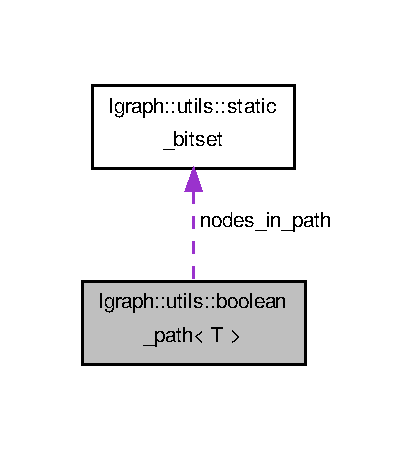
\includegraphics[width=201pt]{classlgraph_1_1utils_1_1boolean__path__coll__graph}
\end{center}
\end{figure}
\subsection*{Public Member Functions}
\begin{DoxyCompactItemize}
\item 
void \hyperlink{classlgraph_1_1utils_1_1boolean__path_a84fbdaa6dd1a06f12dba233de81954a5}{init} (size\+\_\+t n)
\begin{DoxyCompactList}\small\item\em Initialises the path to an empty path within a graph of {\itshape n} nodes. \end{DoxyCompactList}\item 
void \hyperlink{classlgraph_1_1utils_1_1boolean__path_af3d56a9ba3f4f7f8c41d4edfeacaa834}{init} (size\+\_\+t n, const \hyperlink{classlgraph_1_1utils_1_1node__path}{node\+\_\+path}$<$ T $>$ \&vp)
\begin{DoxyCompactList}\small\item\em Initialises the path to a path within a graph of {\itshape n} nodes with the nodes in {\itshape vp}. \end{DoxyCompactList}\item 
void \hyperlink{classlgraph_1_1utils_1_1boolean__path_a77384ff404a3e18f012f01eac407d42a}{clear} ()
\begin{DoxyCompactList}\small\item\em Clears the path. \end{DoxyCompactList}\item 
void \hyperlink{classlgraph_1_1utils_1_1boolean__path_a2b01b133b57845543234d6c48281160f}{add\+\_\+node} (\hyperlink{namespacelgraph_1_1utils_a7bd66ede3805ef121bc2835bd48de0cf}{node} u)
\begin{DoxyCompactList}\small\item\em Adds a node to the path. \end{DoxyCompactList}\item 
void \hyperlink{classlgraph_1_1utils_1_1boolean__path_aef98e91742556f0089bc6eb0e4c856a9}{add\+\_\+length} (const T \&l)
\begin{DoxyCompactList}\small\item\em Accumulates to the current length of the the path the value l. \end{DoxyCompactList}\item 
void \hyperlink{classlgraph_1_1utils_1_1boolean__path_ab097b14785a48662e1f1e6c4bd846b5a}{set\+\_\+length} (const T \&l)
\begin{DoxyCompactList}\small\item\em Sets the current length of the the path the value l. \end{DoxyCompactList}\item 
void \hyperlink{classlgraph_1_1utils_1_1boolean__path_a005364eb88d63910a6e3965548d49197}{concatenate} (const \hyperlink{classlgraph_1_1utils_1_1boolean__path}{boolean\+\_\+path}$<$ T $>$ \&bp)
\begin{DoxyCompactList}\small\item\em Adds to this paths all nodes from bp. \end{DoxyCompactList}\item 
bool \hyperlink{classlgraph_1_1utils_1_1boolean__path_a9f0255a332cef8af3193fd683839d870}{operator\mbox{[}$\,$\mbox{]}} (\hyperlink{namespacelgraph_1_1utils_a7bd66ede3805ef121bc2835bd48de0cf}{node} i) const 
\begin{DoxyCompactList}\small\item\em Check if the i-\/th node is in the path. \end{DoxyCompactList}\item 
\hyperlink{classlgraph_1_1utils_1_1boolean__path}{boolean\+\_\+path} \& \hyperlink{classlgraph_1_1utils_1_1boolean__path_aedf4e03dbf45c2f66c79d01de5977ede}{operator=} (const \hyperlink{classlgraph_1_1utils_1_1boolean__path}{boolean\+\_\+path}$<$ T $>$ \&bp)
\begin{DoxyCompactList}\small\item\em Overrides this boolean path\textquotesingle{}s information with {\itshape bp}. \end{DoxyCompactList}\item 
size\+\_\+t \hyperlink{classlgraph_1_1utils_1_1boolean__path_a783ac5583112896796549774fd9e66c2}{size} () const 
\begin{DoxyCompactList}\small\item\em Returns the number of nodes in the path. \end{DoxyCompactList}\item 
T \hyperlink{classlgraph_1_1utils_1_1boolean__path_a2707b0a596ca58e412b41e70d07ae055}{get\+\_\+length} () const 
\begin{DoxyCompactList}\small\item\em Returns this path\textquotesingle{}s length. \end{DoxyCompactList}\item 
size\+\_\+t \hyperlink{classlgraph_1_1utils_1_1boolean__path_a572b365b3ab1232ca5d6f2fce4cd4519}{potential\+\_\+length} () const 
\begin{DoxyCompactList}\small\item\em Returns the maximum number of nodes that could be in the path. \end{DoxyCompactList}\item 
bool \hyperlink{classlgraph_1_1utils_1_1boolean__path_a4227d034267a760b04fab42f18df107d}{closest\+\_\+next} (const \hyperlink{classlgraph_1_1utils_1_1xxgraph}{xxgraph} $\ast$G, \hyperlink{namespacelgraph_1_1utils_a7bd66ede3805ef121bc2835bd48de0cf}{node} previous, \hyperlink{namespacelgraph_1_1utils_a7bd66ede3805ef121bc2835bd48de0cf}{node} current, \hyperlink{namespacelgraph_1_1utils_a7bd66ede3805ef121bc2835bd48de0cf}{node} \&next) const 
\begin{DoxyCompactList}\small\item\em Looks for the next node in this path taking as a reference the {\itshape previous} and {\itshape current} nodes. \end{DoxyCompactList}\item 
bool \hyperlink{classlgraph_1_1utils_1_1boolean__path_ab38f690dd2b0023ef593aafc1351ff3e}{closest\+\_\+next} (const \hyperlink{classlgraph_1_1utils_1_1xxgraph}{xxgraph} $\ast$G, const vector$<$ bool $>$ \&previous, \hyperlink{namespacelgraph_1_1utils_a7bd66ede3805ef121bc2835bd48de0cf}{node} current, \hyperlink{namespacelgraph_1_1utils_a7bd66ede3805ef121bc2835bd48de0cf}{node} \&next) const 
\begin{DoxyCompactList}\small\item\em Looks for the next node in this path taking as a reference the nodes previously visited and the {\itshape current} node. \end{DoxyCompactList}\item 
\hyperlink{classlgraph_1_1utils_1_1node__path}{node\+\_\+path}$<$ T $>$ \hyperlink{classlgraph_1_1utils_1_1boolean__path_afad52b86e4350e1bc8b832e3c26aae6a}{to\+\_\+node\+\_\+path} (const \hyperlink{classlgraph_1_1utils_1_1xxgraph}{xxgraph} $\ast$G, \hyperlink{namespacelgraph_1_1utils_a7bd66ede3805ef121bc2835bd48de0cf}{node} s) const 
\begin{DoxyCompactList}\small\item\em Converts this \hyperlink{classlgraph_1_1utils_1_1boolean__path}{boolean\+\_\+path} to an object of type \hyperlink{classlgraph_1_1utils_1_1node__path}{node\+\_\+path}. \end{DoxyCompactList}\item 
void \hyperlink{classlgraph_1_1utils_1_1boolean__path_afc30ddbf3f5651336f570c20d5f74f3e}{to\+\_\+node\+\_\+path} (const \hyperlink{classlgraph_1_1utils_1_1xxgraph}{xxgraph} $\ast$G, \hyperlink{namespacelgraph_1_1utils_a7bd66ede3805ef121bc2835bd48de0cf}{node} s, \hyperlink{classlgraph_1_1utils_1_1node__path}{node\+\_\+path}$<$ T $>$ \&np) const 
\begin{DoxyCompactList}\small\item\em Converts this \hyperlink{classlgraph_1_1utils_1_1boolean__path}{boolean\+\_\+path} to an object of type \hyperlink{classlgraph_1_1utils_1_1node__path}{node\+\_\+path}. \end{DoxyCompactList}\item 
string \hyperlink{classlgraph_1_1utils_1_1boolean__path_a3a562317b24dfc0abc3d8eb1e834eceb}{pretty\+\_\+string} () const 
\begin{DoxyCompactList}\small\item\em Formats this path into a string with a \textquotesingle{}pretty\textquotesingle{} format. \end{DoxyCompactList}\item 
void \hyperlink{classlgraph_1_1utils_1_1boolean__path_a772943b08c2cdca78583a2c539093db2}{pretty\+\_\+string} (string \&s) const 
\begin{DoxyCompactList}\small\item\em Formats this path into a string with a \textquotesingle{}pretty\textquotesingle{} format. \end{DoxyCompactList}\item 
string \hyperlink{classlgraph_1_1utils_1_1boolean__path_a3ca892df161835a80430d540ca883ab1}{to\+\_\+string} () const 
\begin{DoxyCompactList}\small\item\em Formats this path into a string with a plain format. \end{DoxyCompactList}\item 
void \hyperlink{classlgraph_1_1utils_1_1boolean__path_a86bbdb236fc31e2abd09f6029548b181}{to\+\_\+string} (string \&s) const 
\begin{DoxyCompactList}\small\item\em Formats this path into a string with a plain format. \end{DoxyCompactList}\end{DoxyCompactItemize}
\subsection*{Private Attributes}
\begin{DoxyCompactItemize}
\item 
\hyperlink{classlgraph_1_1utils_1_1static__bitset}{static\+\_\+bitset} \hyperlink{classlgraph_1_1utils_1_1boolean__path_ab94143c4100d65e2989fb150d6112818}{nodes\+\_\+in\+\_\+path}
\begin{DoxyCompactList}\small\item\em The list of nodes as Boolean values. \end{DoxyCompactList}\item 
size\+\_\+t \hyperlink{classlgraph_1_1utils_1_1boolean__path_a9798bc25ba71adebcd38abe36db471ca}{n\+\_\+nodes}\hypertarget{classlgraph_1_1utils_1_1boolean__path_a9798bc25ba71adebcd38abe36db471ca}{}\label{classlgraph_1_1utils_1_1boolean__path_a9798bc25ba71adebcd38abe36db471ca}

\begin{DoxyCompactList}\small\item\em Number of nodes in the path, i.\+e., the amount of values set to true. \end{DoxyCompactList}\item 
T \hyperlink{classlgraph_1_1utils_1_1boolean__path_a35ff8125a2ef2418feb576d2fe528517}{path\+\_\+length}
\begin{DoxyCompactList}\small\item\em The total weight of this path. \end{DoxyCompactList}\end{DoxyCompactItemize}
\subsection*{Friends}
\begin{DoxyCompactItemize}
\item 
ostream \& \hyperlink{classlgraph_1_1utils_1_1boolean__path_a5f7334ccc188792f571109cd67e73d0d}{operator$<$$<$} (ostream \&os, const \hyperlink{classlgraph_1_1utils_1_1boolean__path}{boolean\+\_\+path}$<$ T $>$ \&bp)
\begin{DoxyCompactList}\small\item\em Outputs this path on a {\itshape ostream} object. \end{DoxyCompactList}\end{DoxyCompactItemize}


\subsection{Detailed Description}
\subsubsection*{template$<$class T = \+\_\+new\+\_\+$>$\\*
class lgraph\+::utils\+::boolean\+\_\+path$<$ T $>$}

A path through a graph seen as a list of Boolean values. 

The i-\/th position of this path is 1 if, and only if, the i-\/th node of the graph is in the path. This is intended to be used O\+N\+LY for shortest paths. Therefore, any \hyperlink{classlgraph_1_1utils_1_1boolean__path}{boolean\+\_\+path} can be converted into a \hyperlink{classlgraph_1_1utils_1_1node__path}{node\+\_\+path} under the following condition\+: if p(u) is the position of node \textquotesingle{}u\textquotesingle{} in the node path then\+:
\begin{DoxyItemize}
\item if u has only one neighbour \textquotesingle{}v\textquotesingle{} then either p(v) $<$ p(u) or p(u) $<$ p(v)
\item if u has two neighbours \textquotesingle{}v\textquotesingle{}, \textquotesingle{}w\textquotesingle{} then either p(v) $<$ p(u) $<$ p(w) or p(w) $<$ p(u) $<$ p(v) Any other boolean path not following the previous two conventions is not guaranteed to be able to be converted into an object of type \textquotesingle{}\hyperlink{classlgraph_1_1utils_1_1node__path}{node\+\_\+path}\textquotesingle{}. The template parameter type is the type used to store this path\textquotesingle{}s length (see \hyperlink{classlgraph_1_1utils_1_1boolean__path_a35ff8125a2ef2418feb576d2fe528517}{path\+\_\+length}).
\end{DoxyItemize}


\begin{DoxyParams}{Parameters}
{\em T} & The type used for the length. It must support comparisons and the C++\textquotesingle{}s output operator $<$$<$. \\
\hline
\end{DoxyParams}


\subsection{Member Function Documentation}
\index{lgraph\+::utils\+::boolean\+\_\+path@{lgraph\+::utils\+::boolean\+\_\+path}!add\+\_\+length@{add\+\_\+length}}
\index{add\+\_\+length@{add\+\_\+length}!lgraph\+::utils\+::boolean\+\_\+path@{lgraph\+::utils\+::boolean\+\_\+path}}
\subsubsection[{\texorpdfstring{add\+\_\+length(const T \&l)}{add_length(const T &l)}}]{\setlength{\rightskip}{0pt plus 5cm}template$<$class T $>$ void {\bf lgraph\+::utils\+::boolean\+\_\+path}$<$ T $>$\+::add\+\_\+length (
\begin{DoxyParamCaption}
\item[{const T \&}]{l}
\end{DoxyParamCaption}
)}\hypertarget{classlgraph_1_1utils_1_1boolean__path_aef98e91742556f0089bc6eb0e4c856a9}{}\label{classlgraph_1_1utils_1_1boolean__path_aef98e91742556f0089bc6eb0e4c856a9}


Accumulates to the current length of the the path the value l. 


\begin{DoxyParams}{Parameters}
{\em l} & The value to be accumulated to \hyperlink{classlgraph_1_1utils_1_1boolean__path_a35ff8125a2ef2418feb576d2fe528517}{path\+\_\+length} \\
\hline
\end{DoxyParams}
\index{lgraph\+::utils\+::boolean\+\_\+path@{lgraph\+::utils\+::boolean\+\_\+path}!add\+\_\+node@{add\+\_\+node}}
\index{add\+\_\+node@{add\+\_\+node}!lgraph\+::utils\+::boolean\+\_\+path@{lgraph\+::utils\+::boolean\+\_\+path}}
\subsubsection[{\texorpdfstring{add\+\_\+node(node u)}{add_node(node u)}}]{\setlength{\rightskip}{0pt plus 5cm}template$<$class T $>$ void {\bf lgraph\+::utils\+::boolean\+\_\+path}$<$ T $>$\+::add\+\_\+node (
\begin{DoxyParamCaption}
\item[{{\bf node}}]{u}
\end{DoxyParamCaption}
)}\hypertarget{classlgraph_1_1utils_1_1boolean__path_a2b01b133b57845543234d6c48281160f}{}\label{classlgraph_1_1utils_1_1boolean__path_a2b01b133b57845543234d6c48281160f}


Adds a node to the path. 

The corresponding position of \hyperlink{classlgraph_1_1utils_1_1boolean__path_ab94143c4100d65e2989fb150d6112818}{nodes\+\_\+in\+\_\+path} is set to true. 
\begin{DoxyParams}{Parameters}
{\em u} & The node\textquotesingle{}s index, between 0 and \hyperlink{classlgraph_1_1utils_1_1boolean__path_a9798bc25ba71adebcd38abe36db471ca}{n\+\_\+nodes} -\/ 1 \\
\hline
\end{DoxyParams}
\begin{DoxyPostcond}{Postcondition}
The length remains unchanged 
\end{DoxyPostcond}
\index{lgraph\+::utils\+::boolean\+\_\+path@{lgraph\+::utils\+::boolean\+\_\+path}!clear@{clear}}
\index{clear@{clear}!lgraph\+::utils\+::boolean\+\_\+path@{lgraph\+::utils\+::boolean\+\_\+path}}
\subsubsection[{\texorpdfstring{clear()}{clear()}}]{\setlength{\rightskip}{0pt plus 5cm}template$<$class T $>$ void {\bf lgraph\+::utils\+::boolean\+\_\+path}$<$ T $>$\+::clear (
\begin{DoxyParamCaption}
{}
\end{DoxyParamCaption}
)}\hypertarget{classlgraph_1_1utils_1_1boolean__path_a77384ff404a3e18f012f01eac407d42a}{}\label{classlgraph_1_1utils_1_1boolean__path_a77384ff404a3e18f012f01eac407d42a}


Clears the path. 

One of the two methods \hyperlink{classlgraph_1_1utils_1_1boolean__path_a84fbdaa6dd1a06f12dba233de81954a5}{init(size\+\_\+t)} or \hyperlink{classlgraph_1_1utils_1_1boolean__path_af3d56a9ba3f4f7f8c41d4edfeacaa834}{init(size\+\_\+t,const node\+\_\+path$<$\+T$>$\&)} will have to be called again to be able to use it again. However, the destructor of this class frees the memory automatically. \index{lgraph\+::utils\+::boolean\+\_\+path@{lgraph\+::utils\+::boolean\+\_\+path}!closest\+\_\+next@{closest\+\_\+next}}
\index{closest\+\_\+next@{closest\+\_\+next}!lgraph\+::utils\+::boolean\+\_\+path@{lgraph\+::utils\+::boolean\+\_\+path}}
\subsubsection[{\texorpdfstring{closest\+\_\+next(const xxgraph $\ast$\+G, node previous, node current, node \&next) const }{closest_next(const xxgraph *G, node previous, node current, node &next) const }}]{\setlength{\rightskip}{0pt plus 5cm}template$<$class T $>$ bool {\bf lgraph\+::utils\+::boolean\+\_\+path}$<$ T $>$\+::closest\+\_\+next (
\begin{DoxyParamCaption}
\item[{const {\bf xxgraph} $\ast$}]{G, }
\item[{{\bf node}}]{previous, }
\item[{{\bf node}}]{current, }
\item[{{\bf node} \&}]{next}
\end{DoxyParamCaption}
) const}\hypertarget{classlgraph_1_1utils_1_1boolean__path_a4227d034267a760b04fab42f18df107d}{}\label{classlgraph_1_1utils_1_1boolean__path_a4227d034267a760b04fab42f18df107d}


Looks for the next node in this path taking as a reference the {\itshape previous} and {\itshape current} nodes. 

Since a node could have more than one of its neighbour in the path, the node that it retrieves is the closest to the {\itshape current} node, that is different from the {\itshape previous} node.


\begin{DoxyParams}[1]{Parameters}
\mbox{\tt in}  & {\em G} & The graph this path goes through. \\
\hline
\mbox{\tt in}  & {\em previous} & The previous node in the path. To retrieve the second node in the path, set this parameter to -\/1. \\
\hline
\mbox{\tt in}  & {\em current} & The current node in the path. \\
\hline
\mbox{\tt out}  & {\em next} & The value of the next node in the path, if it exists. \\
\hline
\end{DoxyParams}
\begin{DoxyReturn}{Returns}
Returns true if there actually exists a \char`\"{}next\char`\"{} node in the path. 
\end{DoxyReturn}
\index{lgraph\+::utils\+::boolean\+\_\+path@{lgraph\+::utils\+::boolean\+\_\+path}!closest\+\_\+next@{closest\+\_\+next}}
\index{closest\+\_\+next@{closest\+\_\+next}!lgraph\+::utils\+::boolean\+\_\+path@{lgraph\+::utils\+::boolean\+\_\+path}}
\subsubsection[{\texorpdfstring{closest\+\_\+next(const xxgraph $\ast$\+G, const vector$<$ bool $>$ \&previous, node current, node \&next) const }{closest_next(const xxgraph *G, const vector< bool > &previous, node current, node &next) const }}]{\setlength{\rightskip}{0pt plus 5cm}template$<$class T $>$ bool {\bf lgraph\+::utils\+::boolean\+\_\+path}$<$ T $>$\+::closest\+\_\+next (
\begin{DoxyParamCaption}
\item[{const {\bf xxgraph} $\ast$}]{G, }
\item[{const vector$<$ bool $>$ \&}]{previous, }
\item[{{\bf node}}]{current, }
\item[{{\bf node} \&}]{next}
\end{DoxyParamCaption}
) const}\hypertarget{classlgraph_1_1utils_1_1boolean__path_ab38f690dd2b0023ef593aafc1351ff3e}{}\label{classlgraph_1_1utils_1_1boolean__path_ab38f690dd2b0023ef593aafc1351ff3e}


Looks for the next node in this path taking as a reference the nodes previously visited and the {\itshape current} node. 

Since a node could have more than one of its neighbour in the path, the node that it retrieves is the closest to the {\itshape current} node, that is different from the previously visited nodes (marked in {\itshape previous}). This function is meant to be used when converting a \hyperlink{classlgraph_1_1utils_1_1boolean__path}{boolean\+\_\+path} to a \hyperlink{classlgraph_1_1utils_1_1node__path}{node\+\_\+path}.


\begin{DoxyParams}[1]{Parameters}
\mbox{\tt in}  & {\em G} & The graph this path goes through. \\
\hline
\mbox{\tt in}  & {\em previous} & The nodes previously visited. To retrieve the second node in the path, all the values must be set to false. Its size must be equal to this path\textquotesingle{}s potential length (see \hyperlink{classlgraph_1_1utils_1_1boolean__path_a572b365b3ab1232ca5d6f2fce4cd4519}{potential\+\_\+length()}). \\
\hline
\mbox{\tt in}  & {\em current} & The current node in the path. \\
\hline
\mbox{\tt out}  & {\em next} & The value of the next node in the path, if it exists. \\
\hline
\end{DoxyParams}
\begin{DoxyReturn}{Returns}
Returns true if there actually exists a \char`\"{}next\char`\"{} node in the path. 
\end{DoxyReturn}
\index{lgraph\+::utils\+::boolean\+\_\+path@{lgraph\+::utils\+::boolean\+\_\+path}!concatenate@{concatenate}}
\index{concatenate@{concatenate}!lgraph\+::utils\+::boolean\+\_\+path@{lgraph\+::utils\+::boolean\+\_\+path}}
\subsubsection[{\texorpdfstring{concatenate(const boolean\+\_\+path$<$ T $>$ \&bp)}{concatenate(const boolean_path< T > &bp)}}]{\setlength{\rightskip}{0pt plus 5cm}template$<$class T $>$ void {\bf lgraph\+::utils\+::boolean\+\_\+path}$<$ T $>$\+::concatenate (
\begin{DoxyParamCaption}
\item[{const {\bf boolean\+\_\+path}$<$ T $>$ \&}]{bp}
\end{DoxyParamCaption}
)}\hypertarget{classlgraph_1_1utils_1_1boolean__path_a005364eb88d63910a6e3965548d49197}{}\label{classlgraph_1_1utils_1_1boolean__path_a005364eb88d63910a6e3965548d49197}


Adds to this paths all nodes from bp. 

All positions in {\itshape bp} set to true will be set to true in this path.


\begin{DoxyParams}{Parameters}
{\em bp} & The boolean path that will be concatenated to this. \\
\hline
\end{DoxyParams}
\begin{DoxyPrecond}{Precondition}
{\itshape bp} must have been initialised with the same value as this. 
\end{DoxyPrecond}
\index{lgraph\+::utils\+::boolean\+\_\+path@{lgraph\+::utils\+::boolean\+\_\+path}!get\+\_\+length@{get\+\_\+length}}
\index{get\+\_\+length@{get\+\_\+length}!lgraph\+::utils\+::boolean\+\_\+path@{lgraph\+::utils\+::boolean\+\_\+path}}
\subsubsection[{\texorpdfstring{get\+\_\+length() const }{get_length() const }}]{\setlength{\rightskip}{0pt plus 5cm}template$<$class T $>$ T {\bf lgraph\+::utils\+::boolean\+\_\+path}$<$ T $>$\+::get\+\_\+length (
\begin{DoxyParamCaption}
{}
\end{DoxyParamCaption}
) const}\hypertarget{classlgraph_1_1utils_1_1boolean__path_a2707b0a596ca58e412b41e70d07ae055}{}\label{classlgraph_1_1utils_1_1boolean__path_a2707b0a596ca58e412b41e70d07ae055}


Returns this path\textquotesingle{}s length. 

Returns the sum of the distances between the nodes in the path, that is, the value \hyperlink{classlgraph_1_1utils_1_1boolean__path_a35ff8125a2ef2418feb576d2fe528517}{path\+\_\+length} \index{lgraph\+::utils\+::boolean\+\_\+path@{lgraph\+::utils\+::boolean\+\_\+path}!init@{init}}
\index{init@{init}!lgraph\+::utils\+::boolean\+\_\+path@{lgraph\+::utils\+::boolean\+\_\+path}}
\subsubsection[{\texorpdfstring{init(size\+\_\+t n)}{init(size_t n)}}]{\setlength{\rightskip}{0pt plus 5cm}template$<$class T $>$ void {\bf lgraph\+::utils\+::boolean\+\_\+path}$<$ T $>$\+::init (
\begin{DoxyParamCaption}
\item[{size\+\_\+t}]{n}
\end{DoxyParamCaption}
)}\hypertarget{classlgraph_1_1utils_1_1boolean__path_a84fbdaa6dd1a06f12dba233de81954a5}{}\label{classlgraph_1_1utils_1_1boolean__path_a84fbdaa6dd1a06f12dba233de81954a5}


Initialises the path to an empty path within a graph of {\itshape n} nodes. 

There is no need for this path to be \textquotesingle{}uninitialised\textquotesingle{}. \index{lgraph\+::utils\+::boolean\+\_\+path@{lgraph\+::utils\+::boolean\+\_\+path}!init@{init}}
\index{init@{init}!lgraph\+::utils\+::boolean\+\_\+path@{lgraph\+::utils\+::boolean\+\_\+path}}
\subsubsection[{\texorpdfstring{init(size\+\_\+t n, const node\+\_\+path$<$ T $>$ \&vp)}{init(size_t n, const node_path< T > &vp)}}]{\setlength{\rightskip}{0pt plus 5cm}template$<$class T $>$ void {\bf lgraph\+::utils\+::boolean\+\_\+path}$<$ T $>$\+::init (
\begin{DoxyParamCaption}
\item[{size\+\_\+t}]{n, }
\item[{const {\bf node\+\_\+path}$<$ T $>$ \&}]{vp}
\end{DoxyParamCaption}
)}\hypertarget{classlgraph_1_1utils_1_1boolean__path_af3d56a9ba3f4f7f8c41d4edfeacaa834}{}\label{classlgraph_1_1utils_1_1boolean__path_af3d56a9ba3f4f7f8c41d4edfeacaa834}


Initialises the path to a path within a graph of {\itshape n} nodes with the nodes in {\itshape vp}. 


\begin{DoxyParams}{Parameters}
{\em n} & The number of nodes of the graph this path goes through. \\
\hline
{\em vp} & The list of nodes that makes the path within the graph. All indices of this path must be lower than {\itshape n}. \\
\hline
\end{DoxyParams}
\index{lgraph\+::utils\+::boolean\+\_\+path@{lgraph\+::utils\+::boolean\+\_\+path}!operator=@{operator=}}
\index{operator=@{operator=}!lgraph\+::utils\+::boolean\+\_\+path@{lgraph\+::utils\+::boolean\+\_\+path}}
\subsubsection[{\texorpdfstring{operator=(const boolean\+\_\+path$<$ T $>$ \&bp)}{operator=(const boolean_path< T > &bp)}}]{\setlength{\rightskip}{0pt plus 5cm}template$<$class T $>$ {\bf boolean\+\_\+path}$<$ T $>$ \& {\bf lgraph\+::utils\+::boolean\+\_\+path}$<$ T $>$\+::operator= (
\begin{DoxyParamCaption}
\item[{const {\bf boolean\+\_\+path}$<$ T $>$ \&}]{bp}
\end{DoxyParamCaption}
)}\hypertarget{classlgraph_1_1utils_1_1boolean__path_aedf4e03dbf45c2f66c79d01de5977ede}{}\label{classlgraph_1_1utils_1_1boolean__path_aedf4e03dbf45c2f66c79d01de5977ede}


Overrides this boolean path\textquotesingle{}s information with {\itshape bp}. 

This boolean path\textquotesingle{}s memory is first freed and reallocated to hold the contents in {\itshape bp}.


\begin{DoxyParams}{Parameters}
{\em bp} & The new boolean path. \\
\hline
\end{DoxyParams}
\index{lgraph\+::utils\+::boolean\+\_\+path@{lgraph\+::utils\+::boolean\+\_\+path}!operator\mbox{[}$\,$\mbox{]}@{operator[]}}
\index{operator\mbox{[}$\,$\mbox{]}@{operator[]}!lgraph\+::utils\+::boolean\+\_\+path@{lgraph\+::utils\+::boolean\+\_\+path}}
\subsubsection[{\texorpdfstring{operator[](node i) const }{operator[](node i) const }}]{\setlength{\rightskip}{0pt plus 5cm}template$<$class T $>$ bool {\bf lgraph\+::utils\+::boolean\+\_\+path}$<$ T $>$\+::operator\mbox{[}$\,$\mbox{]} (
\begin{DoxyParamCaption}
\item[{{\bf node}}]{i}
\end{DoxyParamCaption}
) const}\hypertarget{classlgraph_1_1utils_1_1boolean__path_a9f0255a332cef8af3193fd683839d870}{}\label{classlgraph_1_1utils_1_1boolean__path_a9f0255a332cef8af3193fd683839d870}


Check if the i-\/th node is in the path. 


\begin{DoxyParams}{Parameters}
{\em i} & The node\textquotesingle{}s index. \\
\hline
\end{DoxyParams}
\begin{DoxyReturn}{Returns}
Returns true if, and only if, \hyperlink{classlgraph_1_1utils_1_1boolean__path_ab94143c4100d65e2989fb150d6112818}{nodes\+\_\+in\+\_\+path}\mbox{[}{\itshape i}\mbox{]} is set to true. 
\end{DoxyReturn}
\begin{DoxyPrecond}{Precondition}
The node index {\itshape i} must satisfy {\itshape i} $<$ \hyperlink{classlgraph_1_1utils_1_1boolean__path_a9798bc25ba71adebcd38abe36db471ca}{n\+\_\+nodes} 
\end{DoxyPrecond}
\index{lgraph\+::utils\+::boolean\+\_\+path@{lgraph\+::utils\+::boolean\+\_\+path}!potential\+\_\+length@{potential\+\_\+length}}
\index{potential\+\_\+length@{potential\+\_\+length}!lgraph\+::utils\+::boolean\+\_\+path@{lgraph\+::utils\+::boolean\+\_\+path}}
\subsubsection[{\texorpdfstring{potential\+\_\+length() const }{potential_length() const }}]{\setlength{\rightskip}{0pt plus 5cm}template$<$class T $>$ size\+\_\+t {\bf lgraph\+::utils\+::boolean\+\_\+path}$<$ T $>$\+::potential\+\_\+length (
\begin{DoxyParamCaption}
{}
\end{DoxyParamCaption}
) const}\hypertarget{classlgraph_1_1utils_1_1boolean__path_a572b365b3ab1232ca5d6f2fce4cd4519}{}\label{classlgraph_1_1utils_1_1boolean__path_a572b365b3ab1232ca5d6f2fce4cd4519}


Returns the maximum number of nodes that could be in the path. 

Basically, returns the size used to initialise it. \index{lgraph\+::utils\+::boolean\+\_\+path@{lgraph\+::utils\+::boolean\+\_\+path}!pretty\+\_\+string@{pretty\+\_\+string}}
\index{pretty\+\_\+string@{pretty\+\_\+string}!lgraph\+::utils\+::boolean\+\_\+path@{lgraph\+::utils\+::boolean\+\_\+path}}
\subsubsection[{\texorpdfstring{pretty\+\_\+string() const }{pretty_string() const }}]{\setlength{\rightskip}{0pt plus 5cm}template$<$class T $>$ string {\bf lgraph\+::utils\+::boolean\+\_\+path}$<$ T $>$\+::pretty\+\_\+string (
\begin{DoxyParamCaption}
{}
\end{DoxyParamCaption}
) const}\hypertarget{classlgraph_1_1utils_1_1boolean__path_a3a562317b24dfc0abc3d8eb1e834eceb}{}\label{classlgraph_1_1utils_1_1boolean__path_a3a562317b24dfc0abc3d8eb1e834eceb}


Formats this path into a string with a \textquotesingle{}pretty\textquotesingle{} format. 

\begin{DoxyReturn}{Returns}
Returns this path formatted into a string that has two parts separated with an \textquotesingle{}endl\textquotesingle{} character. The first is the header indicating the index of the node. The second is either a 0 or a 1 telling whether the corresponding index is in the path or not. 
\end{DoxyReturn}
\index{lgraph\+::utils\+::boolean\+\_\+path@{lgraph\+::utils\+::boolean\+\_\+path}!pretty\+\_\+string@{pretty\+\_\+string}}
\index{pretty\+\_\+string@{pretty\+\_\+string}!lgraph\+::utils\+::boolean\+\_\+path@{lgraph\+::utils\+::boolean\+\_\+path}}
\subsubsection[{\texorpdfstring{pretty\+\_\+string(string \&s) const }{pretty_string(string &s) const }}]{\setlength{\rightskip}{0pt plus 5cm}template$<$class T $>$ void {\bf lgraph\+::utils\+::boolean\+\_\+path}$<$ T $>$\+::pretty\+\_\+string (
\begin{DoxyParamCaption}
\item[{string \&}]{s}
\end{DoxyParamCaption}
) const}\hypertarget{classlgraph_1_1utils_1_1boolean__path_a772943b08c2cdca78583a2c539093db2}{}\label{classlgraph_1_1utils_1_1boolean__path_a772943b08c2cdca78583a2c539093db2}


Formats this path into a string with a \textquotesingle{}pretty\textquotesingle{} format. 


\begin{DoxyParams}[1]{Parameters}
\mbox{\tt out}  & {\em s} & Stores this path formatted into a string that has two parts separated with an \textquotesingle{}endl\textquotesingle{} character. The first is the header indicating the index of the node. The second is either a 0 or a 1 telling whether the corresponding index is in the path or not. \\
\hline
\end{DoxyParams}
\index{lgraph\+::utils\+::boolean\+\_\+path@{lgraph\+::utils\+::boolean\+\_\+path}!set\+\_\+length@{set\+\_\+length}}
\index{set\+\_\+length@{set\+\_\+length}!lgraph\+::utils\+::boolean\+\_\+path@{lgraph\+::utils\+::boolean\+\_\+path}}
\subsubsection[{\texorpdfstring{set\+\_\+length(const T \&l)}{set_length(const T &l)}}]{\setlength{\rightskip}{0pt plus 5cm}template$<$class T $>$ void {\bf lgraph\+::utils\+::boolean\+\_\+path}$<$ T $>$\+::set\+\_\+length (
\begin{DoxyParamCaption}
\item[{const T \&}]{l}
\end{DoxyParamCaption}
)}\hypertarget{classlgraph_1_1utils_1_1boolean__path_ab097b14785a48662e1f1e6c4bd846b5a}{}\label{classlgraph_1_1utils_1_1boolean__path_ab097b14785a48662e1f1e6c4bd846b5a}


Sets the current length of the the path the value l. 


\begin{DoxyParams}{Parameters}
{\em l} & The value that will replace the current value of \hyperlink{classlgraph_1_1utils_1_1boolean__path_a35ff8125a2ef2418feb576d2fe528517}{path\+\_\+length} \\
\hline
\end{DoxyParams}
\index{lgraph\+::utils\+::boolean\+\_\+path@{lgraph\+::utils\+::boolean\+\_\+path}!size@{size}}
\index{size@{size}!lgraph\+::utils\+::boolean\+\_\+path@{lgraph\+::utils\+::boolean\+\_\+path}}
\subsubsection[{\texorpdfstring{size() const }{size() const }}]{\setlength{\rightskip}{0pt plus 5cm}template$<$class T $>$ size\+\_\+t {\bf lgraph\+::utils\+::boolean\+\_\+path}$<$ T $>$\+::size (
\begin{DoxyParamCaption}
{}
\end{DoxyParamCaption}
) const}\hypertarget{classlgraph_1_1utils_1_1boolean__path_a783ac5583112896796549774fd9e66c2}{}\label{classlgraph_1_1utils_1_1boolean__path_a783ac5583112896796549774fd9e66c2}


Returns the number of nodes in the path. 

Returns the value \hyperlink{classlgraph_1_1utils_1_1boolean__path_a9798bc25ba71adebcd38abe36db471ca}{n\+\_\+nodes} \index{lgraph\+::utils\+::boolean\+\_\+path@{lgraph\+::utils\+::boolean\+\_\+path}!to\+\_\+node\+\_\+path@{to\+\_\+node\+\_\+path}}
\index{to\+\_\+node\+\_\+path@{to\+\_\+node\+\_\+path}!lgraph\+::utils\+::boolean\+\_\+path@{lgraph\+::utils\+::boolean\+\_\+path}}
\subsubsection[{\texorpdfstring{to\+\_\+node\+\_\+path(const xxgraph $\ast$\+G, node s) const }{to_node_path(const xxgraph *G, node s) const }}]{\setlength{\rightskip}{0pt plus 5cm}template$<$class T $>$ {\bf node\+\_\+path}$<$ T $>$ {\bf lgraph\+::utils\+::boolean\+\_\+path}$<$ T $>$\+::to\+\_\+node\+\_\+path (
\begin{DoxyParamCaption}
\item[{const {\bf xxgraph} $\ast$}]{G, }
\item[{{\bf node}}]{s}
\end{DoxyParamCaption}
) const}\hypertarget{classlgraph_1_1utils_1_1boolean__path_afad52b86e4350e1bc8b832e3c26aae6a}{}\label{classlgraph_1_1utils_1_1boolean__path_afad52b86e4350e1bc8b832e3c26aae6a}


Converts this \hyperlink{classlgraph_1_1utils_1_1boolean__path}{boolean\+\_\+path} to an object of type \hyperlink{classlgraph_1_1utils_1_1node__path}{node\+\_\+path}. 

The conversion is done assuming that the \hyperlink{classlgraph_1_1utils_1_1boolean__path}{boolean\+\_\+path} starts at node {\itshape s}. The result is an object that stores the path as a list of nodes.


\begin{DoxyParams}{Parameters}
{\em G} & The graph this path goes through. \\
\hline
{\em s} & The node where this path starts at. \\
\hline
\end{DoxyParams}
\begin{DoxyReturn}{Returns}
Returns a \hyperlink{classlgraph_1_1utils_1_1node__path}{node\+\_\+path} object equivalent to this boolean path. 
\end{DoxyReturn}
\index{lgraph\+::utils\+::boolean\+\_\+path@{lgraph\+::utils\+::boolean\+\_\+path}!to\+\_\+node\+\_\+path@{to\+\_\+node\+\_\+path}}
\index{to\+\_\+node\+\_\+path@{to\+\_\+node\+\_\+path}!lgraph\+::utils\+::boolean\+\_\+path@{lgraph\+::utils\+::boolean\+\_\+path}}
\subsubsection[{\texorpdfstring{to\+\_\+node\+\_\+path(const xxgraph $\ast$\+G, node s, node\+\_\+path$<$ T $>$ \&np) const }{to_node_path(const xxgraph *G, node s, node_path< T > &np) const }}]{\setlength{\rightskip}{0pt plus 5cm}template$<$class T $>$ void {\bf lgraph\+::utils\+::boolean\+\_\+path}$<$ T $>$\+::to\+\_\+node\+\_\+path (
\begin{DoxyParamCaption}
\item[{const {\bf xxgraph} $\ast$}]{G, }
\item[{{\bf node}}]{s, }
\item[{{\bf node\+\_\+path}$<$ T $>$ \&}]{np}
\end{DoxyParamCaption}
) const}\hypertarget{classlgraph_1_1utils_1_1boolean__path_afc30ddbf3f5651336f570c20d5f74f3e}{}\label{classlgraph_1_1utils_1_1boolean__path_afc30ddbf3f5651336f570c20d5f74f3e}


Converts this \hyperlink{classlgraph_1_1utils_1_1boolean__path}{boolean\+\_\+path} to an object of type \hyperlink{classlgraph_1_1utils_1_1node__path}{node\+\_\+path}. 

The conversion is done assuming that the \hyperlink{classlgraph_1_1utils_1_1boolean__path}{boolean\+\_\+path} starts at node {\itshape s}. The result is an object that stores the path as a list of nodes.


\begin{DoxyParams}[1]{Parameters}
\mbox{\tt in}  & {\em G} & The graph this path goes through. \\
\hline
\mbox{\tt in}  & {\em s} & The node where this path starts at. \\
\hline
\mbox{\tt out}  & {\em np} & The path seen as a list of nodes. \\
\hline
\end{DoxyParams}
\index{lgraph\+::utils\+::boolean\+\_\+path@{lgraph\+::utils\+::boolean\+\_\+path}!to\+\_\+string@{to\+\_\+string}}
\index{to\+\_\+string@{to\+\_\+string}!lgraph\+::utils\+::boolean\+\_\+path@{lgraph\+::utils\+::boolean\+\_\+path}}
\subsubsection[{\texorpdfstring{to\+\_\+string() const }{to_string() const }}]{\setlength{\rightskip}{0pt plus 5cm}template$<$class T $>$ string {\bf lgraph\+::utils\+::boolean\+\_\+path}$<$ T $>$\+::to\+\_\+string (
\begin{DoxyParamCaption}
{}
\end{DoxyParamCaption}
) const}\hypertarget{classlgraph_1_1utils_1_1boolean__path_a3ca892df161835a80430d540ca883ab1}{}\label{classlgraph_1_1utils_1_1boolean__path_a3ca892df161835a80430d540ca883ab1}


Formats this path into a string with a plain format. 

\begin{DoxyReturn}{Returns}
Returns this path as a list of 0\textquotesingle{}s and 1\textquotesingle{}s. The i-\/th digit is a 1 if, and only if, the i-\/th vertex is in the path. 
\end{DoxyReturn}
\index{lgraph\+::utils\+::boolean\+\_\+path@{lgraph\+::utils\+::boolean\+\_\+path}!to\+\_\+string@{to\+\_\+string}}
\index{to\+\_\+string@{to\+\_\+string}!lgraph\+::utils\+::boolean\+\_\+path@{lgraph\+::utils\+::boolean\+\_\+path}}
\subsubsection[{\texorpdfstring{to\+\_\+string(string \&s) const }{to_string(string &s) const }}]{\setlength{\rightskip}{0pt plus 5cm}template$<$class T $>$ void {\bf lgraph\+::utils\+::boolean\+\_\+path}$<$ T $>$\+::to\+\_\+string (
\begin{DoxyParamCaption}
\item[{string \&}]{s}
\end{DoxyParamCaption}
) const}\hypertarget{classlgraph_1_1utils_1_1boolean__path_a86bbdb236fc31e2abd09f6029548b181}{}\label{classlgraph_1_1utils_1_1boolean__path_a86bbdb236fc31e2abd09f6029548b181}


Formats this path into a string with a plain format. 


\begin{DoxyParams}[1]{Parameters}
\mbox{\tt out}  & {\em s} & Stores this path as a list of 0\textquotesingle{}s and 1\textquotesingle{}s. The i-\/th digit is a 1 if, and only if, the i-\/th vertex is in the path. \\
\hline
\end{DoxyParams}


\subsection{Friends And Related Function Documentation}
\index{lgraph\+::utils\+::boolean\+\_\+path@{lgraph\+::utils\+::boolean\+\_\+path}!operator$<$$<$@{operator$<$$<$}}
\index{operator$<$$<$@{operator$<$$<$}!lgraph\+::utils\+::boolean\+\_\+path@{lgraph\+::utils\+::boolean\+\_\+path}}
\subsubsection[{\texorpdfstring{operator$<$$<$}{operator<<}}]{\setlength{\rightskip}{0pt plus 5cm}template$<$class T = \+\_\+new\+\_\+$>$ ostream\& operator$<$$<$ (
\begin{DoxyParamCaption}
\item[{ostream \&}]{os, }
\item[{const {\bf boolean\+\_\+path}$<$ T $>$ \&}]{bp}
\end{DoxyParamCaption}
)\hspace{0.3cm}{\ttfamily [friend]}}\hypertarget{classlgraph_1_1utils_1_1boolean__path_a5f7334ccc188792f571109cd67e73d0d}{}\label{classlgraph_1_1utils_1_1boolean__path_a5f7334ccc188792f571109cd67e73d0d}


Outputs this path on a {\itshape ostream} object. 

The format is this path as a string (see \hyperlink{classlgraph_1_1utils_1_1boolean__path_a3ca892df161835a80430d540ca883ab1}{to\+\_\+string()}) followed by \textquotesingle{}-\/$>$\textquotesingle{} and this path\textquotesingle{}s length. 

\subsection{Member Data Documentation}
\index{lgraph\+::utils\+::boolean\+\_\+path@{lgraph\+::utils\+::boolean\+\_\+path}!nodes\+\_\+in\+\_\+path@{nodes\+\_\+in\+\_\+path}}
\index{nodes\+\_\+in\+\_\+path@{nodes\+\_\+in\+\_\+path}!lgraph\+::utils\+::boolean\+\_\+path@{lgraph\+::utils\+::boolean\+\_\+path}}
\subsubsection[{\texorpdfstring{nodes\+\_\+in\+\_\+path}{nodes_in_path}}]{\setlength{\rightskip}{0pt plus 5cm}template$<$class T = \+\_\+new\+\_\+$>$ {\bf static\+\_\+bitset} {\bf lgraph\+::utils\+::boolean\+\_\+path}$<$ T $>$\+::nodes\+\_\+in\+\_\+path\hspace{0.3cm}{\ttfamily [private]}}\hypertarget{classlgraph_1_1utils_1_1boolean__path_ab94143c4100d65e2989fb150d6112818}{}\label{classlgraph_1_1utils_1_1boolean__path_ab94143c4100d65e2989fb150d6112818}


The list of nodes as Boolean values. 

\hyperlink{classlgraph_1_1utils_1_1boolean__path_ab94143c4100d65e2989fb150d6112818}{nodes\+\_\+in\+\_\+path}\mbox{[}i\mbox{]} = true if, and only if, i-\/th node of the graph is in the path \index{lgraph\+::utils\+::boolean\+\_\+path@{lgraph\+::utils\+::boolean\+\_\+path}!path\+\_\+length@{path\+\_\+length}}
\index{path\+\_\+length@{path\+\_\+length}!lgraph\+::utils\+::boolean\+\_\+path@{lgraph\+::utils\+::boolean\+\_\+path}}
\subsubsection[{\texorpdfstring{path\+\_\+length}{path_length}}]{\setlength{\rightskip}{0pt plus 5cm}template$<$class T = \+\_\+new\+\_\+$>$ T {\bf lgraph\+::utils\+::boolean\+\_\+path}$<$ T $>$\+::path\+\_\+length\hspace{0.3cm}{\ttfamily [private]}}\hypertarget{classlgraph_1_1utils_1_1boolean__path_a35ff8125a2ef2418feb576d2fe528517}{}\label{classlgraph_1_1utils_1_1boolean__path_a35ff8125a2ef2418feb576d2fe528517}


The total weight of this path. 

If \textquotesingle{}p\textquotesingle{} is the path as a list of edges, then \textquotesingle{}path\+\_\+length\textquotesingle{} equals the sum of weights of all edges in \textquotesingle{}p\textquotesingle{}. 

The documentation for this class was generated from the following files\+:\begin{DoxyCompactItemize}
\item 
lgraph/data\+\_\+structures/boolean\+\_\+path.\+hpp\item 
lgraph/data\+\_\+structures/boolean\+\_\+path.\+cpp\end{DoxyCompactItemize}

\hypertarget{classlgraph_1_1utils_1_1cerr__stream}{}\section{lgraph\+:\+:utils\+:\+:cerr\+\_\+stream Class Reference}
\label{classlgraph_1_1utils_1_1cerr__stream}\index{lgraph\+::utils\+::cerr\+\_\+stream@{lgraph\+::utils\+::cerr\+\_\+stream}}


A class for the cerr stream.  




{\ttfamily \#include $<$logger.\+hpp$>$}

\subsection*{Public Types}
\begin{DoxyCompactItemize}
\item 
typedef std\+::basic\+\_\+ostream$<$ char, std\+::char\+\_\+traits$<$ char $>$ $>$ {\bfseries cerr\+\_\+type}\hypertarget{classlgraph_1_1utils_1_1cerr__stream_a60b0847503d146249b71e70473740f57}{}\label{classlgraph_1_1utils_1_1cerr__stream_a60b0847503d146249b71e70473740f57}

\item 
typedef cerr\+\_\+type \&($\ast$ {\bfseries standard\+\_\+endl}) (cerr\+\_\+type \&)\hypertarget{classlgraph_1_1utils_1_1cerr__stream_a8b7e7603a4e656bd2d9196ae0f530c7b}{}\label{classlgraph_1_1utils_1_1cerr__stream_a8b7e7603a4e656bd2d9196ae0f530c7b}

\end{DoxyCompactItemize}
\subsection*{Public Member Functions}
\begin{DoxyCompactItemize}
\item 
void {\bfseries open} (const char $\ast$, const std\+::ios\+\_\+base\+::openmode \&)\hypertarget{classlgraph_1_1utils_1_1cerr__stream_aaec9df1b58756fcda596e29bbfcefeac}{}\label{classlgraph_1_1utils_1_1cerr__stream_aaec9df1b58756fcda596e29bbfcefeac}

\item 
\hyperlink{classlgraph_1_1utils_1_1cerr__stream}{cerr\+\_\+stream} \& {\bfseries operator$<$$<$} (const standard\+\_\+endl \&)\hypertarget{classlgraph_1_1utils_1_1cerr__stream_afd3014b9b67c23c7c86513c0f4969723}{}\label{classlgraph_1_1utils_1_1cerr__stream_afd3014b9b67c23c7c86513c0f4969723}

\item 
{\footnotesize template$<$class t\+\_\+printable $>$ }\\\hyperlink{classlgraph_1_1utils_1_1cerr__stream}{cerr\+\_\+stream} \& {\bfseries operator$<$$<$} (const t\+\_\+printable \&t)\hypertarget{classlgraph_1_1utils_1_1cerr__stream_afd9313105917714104d41bb3990ab81c}{}\label{classlgraph_1_1utils_1_1cerr__stream_afd9313105917714104d41bb3990ab81c}

\end{DoxyCompactItemize}


\subsection{Detailed Description}
A class for the cerr stream. 

A wrapper over the ostrem object cerr. 

The documentation for this class was generated from the following file\+:\begin{DoxyCompactItemize}
\item 
lgraph/utils/logger.\+hpp\end{DoxyCompactItemize}

\hypertarget{classlgraph_1_1utils_1_1cout__stream}{\section{lgraph\-:\-:utils\-:\-:cout\-\_\-stream Class Reference}
\label{classlgraph_1_1utils_1_1cout__stream}\index{lgraph\-::utils\-::cout\-\_\-stream@{lgraph\-::utils\-::cout\-\_\-stream}}
}


A class for the cout stream.  




{\ttfamily \#include $<$logger.\-hpp$>$}

\subsection*{Public Types}
\begin{DoxyCompactItemize}
\item 
\hypertarget{classlgraph_1_1utils_1_1cout__stream_a567e84e8f695f9f06e25a90385bd36bc}{typedef std\-::basic\-\_\-ostream\\*
$<$ char, std\-::char\-\_\-traits$<$ char $>$ $>$ \hyperlink{classlgraph_1_1utils_1_1cout__stream_a567e84e8f695f9f06e25a90385bd36bc}{cout\-\_\-type}}\label{classlgraph_1_1utils_1_1cout__stream_a567e84e8f695f9f06e25a90385bd36bc}

\begin{DoxyCompactList}\small\item\em This is the type of std\-::cout. \end{DoxyCompactList}\item 
\hypertarget{classlgraph_1_1utils_1_1cout__stream_a8d78b6d03f5ae2ffbdc9f859dfe039b3}{typedef \hyperlink{classlgraph_1_1utils_1_1cout__stream_a567e84e8f695f9f06e25a90385bd36bc}{cout\-\_\-type} \&($\ast$ \hyperlink{classlgraph_1_1utils_1_1cout__stream_a8d78b6d03f5ae2ffbdc9f859dfe039b3}{standard\-\_\-endl} )(\hyperlink{classlgraph_1_1utils_1_1cout__stream_a567e84e8f695f9f06e25a90385bd36bc}{cout\-\_\-type} \&)}\label{classlgraph_1_1utils_1_1cout__stream_a8d78b6d03f5ae2ffbdc9f859dfe039b3}

\begin{DoxyCompactList}\small\item\em This is the function signature of std\-::endl. \end{DoxyCompactList}\end{DoxyCompactItemize}
\subsection*{Public Member Functions}
\begin{DoxyCompactItemize}
\item 
\hypertarget{classlgraph_1_1utils_1_1cout__stream_a818a63700e577a13db63088353ce4098}{void \hyperlink{classlgraph_1_1utils_1_1cout__stream_a818a63700e577a13db63088353ce4098}{open} (const char $\ast$, const std\-::ios\-\_\-base\-::openmode \&)}\label{classlgraph_1_1utils_1_1cout__stream_a818a63700e577a13db63088353ce4098}

\begin{DoxyCompactList}\small\item\em Open an empty stream for standard output messages. \end{DoxyCompactList}\item 
\hypertarget{classlgraph_1_1utils_1_1cout__stream_a6e35f97a622bccec72247d6f9e6ca2c8}{\hyperlink{classlgraph_1_1utils_1_1cout__stream}{cout\-\_\-stream} \& \hyperlink{classlgraph_1_1utils_1_1cout__stream_a6e35f97a622bccec72247d6f9e6ca2c8}{operator$<$$<$} (const \hyperlink{classlgraph_1_1utils_1_1cout__stream_a8d78b6d03f5ae2ffbdc9f859dfe039b3}{standard\-\_\-endl} \&)}\label{classlgraph_1_1utils_1_1cout__stream_a6e35f97a622bccec72247d6f9e6ca2c8}

\begin{DoxyCompactList}\small\item\em Define an operator$<$$<$ to take in std\-::endl. \end{DoxyCompactList}\item 
\hypertarget{classlgraph_1_1utils_1_1cout__stream_a88f6cf6d54312f795ccbff57724d51e4}{{\footnotesize template$<$class t\-\_\-printable $>$ }\\\hyperlink{classlgraph_1_1utils_1_1cout__stream}{cout\-\_\-stream} \& \hyperlink{classlgraph_1_1utils_1_1cout__stream_a88f6cf6d54312f795ccbff57724d51e4}{operator$<$$<$} (const t\-\_\-printable \&t)}\label{classlgraph_1_1utils_1_1cout__stream_a88f6cf6d54312f795ccbff57724d51e4}

\begin{DoxyCompactList}\small\item\em operator$<$$<$ for any printable type. \end{DoxyCompactList}\end{DoxyCompactItemize}


\subsection{Detailed Description}
A class for the cout stream. 

A wrapper over the ostrem object cout. 

The documentation for this class was generated from the following file\-:\begin{DoxyCompactItemize}
\item 
lgraph/utils/logger.\-hpp\end{DoxyCompactItemize}

\hypertarget{classlgraph_1_1utils_1_1crandom__generator}{}\section{lgraph\+:\+:utils\+:\+:crandom\+\_\+generator$<$ G, cT $>$ Class Template Reference}
\label{classlgraph_1_1utils_1_1crandom__generator}\index{lgraph\+::utils\+::crandom\+\_\+generator$<$ G, c\+T $>$@{lgraph\+::utils\+::crandom\+\_\+generator$<$ G, c\+T $>$}}


Continuous pseudo-\/\+Random Number Generator (C\+R\+NG).  




{\ttfamily \#include $<$random\+\_\+generator.\+hpp$>$}



Inheritance diagram for lgraph\+:\+:utils\+:\+:crandom\+\_\+generator$<$ G, cT $>$\+:\nopagebreak
\begin{figure}[H]
\begin{center}
\leavevmode
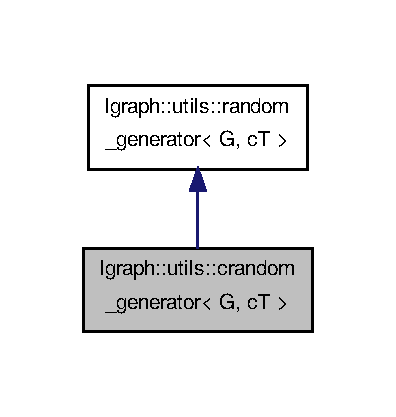
\includegraphics[width=190pt]{classlgraph_1_1utils_1_1crandom__generator__inherit__graph}
\end{center}
\end{figure}


Collaboration diagram for lgraph\+:\+:utils\+:\+:crandom\+\_\+generator$<$ G, cT $>$\+:\nopagebreak
\begin{figure}[H]
\begin{center}
\leavevmode
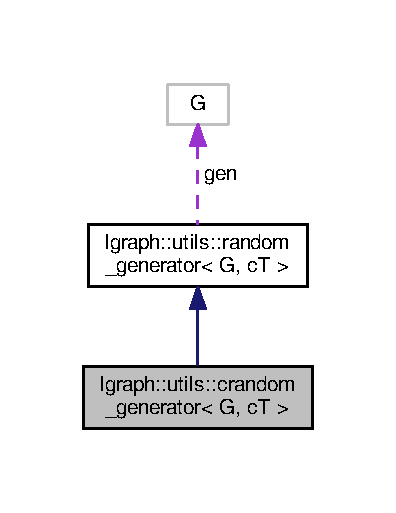
\includegraphics[width=190pt]{classlgraph_1_1utils_1_1crandom__generator__coll__graph}
\end{center}
\end{figure}
\subsection*{Public Member Functions}
\begin{DoxyCompactItemize}
\item 
\mbox{\Hypertarget{classlgraph_1_1utils_1_1crandom__generator_a90bfc340dcb2fa15e744cff6e280978a}\label{classlgraph_1_1utils_1_1crandom__generator_a90bfc340dcb2fa15e744cff6e280978a}} 
\hyperlink{classlgraph_1_1utils_1_1crandom__generator_a90bfc340dcb2fa15e744cff6e280978a}{crandom\+\_\+generator} ()
\begin{DoxyCompactList}\small\item\em Constructor. \end{DoxyCompactList}\item 
\mbox{\Hypertarget{classlgraph_1_1utils_1_1crandom__generator_ade03d6aba0a68ba5b34582cf8107b7aa}\label{classlgraph_1_1utils_1_1crandom__generator_ade03d6aba0a68ba5b34582cf8107b7aa}} 
\hyperlink{classlgraph_1_1utils_1_1crandom__generator_ade03d6aba0a68ba5b34582cf8107b7aa}{$\sim$crandom\+\_\+generator} ()
\begin{DoxyCompactList}\small\item\em Destructor. \end{DoxyCompactList}\item 
void \hyperlink{classlgraph_1_1utils_1_1crandom__generator_addfa5951276296b2a164e5dc482728ce}{init\+\_\+uniform} (cT a, cT b)
\begin{DoxyCompactList}\small\item\em Initialise the uniform distribution. \end{DoxyCompactList}\item 
\mbox{\Hypertarget{classlgraph_1_1utils_1_1crandom__generator_a4d7042cb0862c3b8b4792890e6c5388c}\label{classlgraph_1_1utils_1_1crandom__generator_a4d7042cb0862c3b8b4792890e6c5388c}} 
void \hyperlink{classlgraph_1_1utils_1_1crandom__generator_a4d7042cb0862c3b8b4792890e6c5388c}{init\+\_\+binomial} (cT a, double p)
\begin{DoxyCompactList}\small\item\em The C\+R\+NG leaves this method\textquotesingle{}s body empty. \end{DoxyCompactList}\item 
\mbox{\Hypertarget{classlgraph_1_1utils_1_1crandom__generator_a39dd7f9d80fd5be685cc240719050119}\label{classlgraph_1_1utils_1_1crandom__generator_a39dd7f9d80fd5be685cc240719050119}} 
cT \hyperlink{classlgraph_1_1utils_1_1crandom__generator_a39dd7f9d80fd5be685cc240719050119}{get\+\_\+uniform} ()
\begin{DoxyCompactList}\small\item\em Compute a pseudo-\/random number uniformly at random. \end{DoxyCompactList}\item 
\mbox{\Hypertarget{classlgraph_1_1utils_1_1crandom__generator_ac1f724180b858b6a1f67451060de6896}\label{classlgraph_1_1utils_1_1crandom__generator_ac1f724180b858b6a1f67451060de6896}} 
cT \hyperlink{classlgraph_1_1utils_1_1crandom__generator_ac1f724180b858b6a1f67451060de6896}{get\+\_\+binomial} ()
\begin{DoxyCompactList}\small\item\em In the C\+R\+NG this method always returns 0. \end{DoxyCompactList}\item 
\mbox{\Hypertarget{classlgraph_1_1utils_1_1random__generator_a4eb6998070eecb59bd89dca92d8a509c}\label{classlgraph_1_1utils_1_1random__generator_a4eb6998070eecb59bd89dca92d8a509c}} 
virtual void \hyperlink{classlgraph_1_1utils_1_1random__generator_a4eb6998070eecb59bd89dca92d8a509c}{seed\+\_\+random\+\_\+engine} ()
\begin{DoxyCompactList}\small\item\em Initialises the random engine. \end{DoxyCompactList}\end{DoxyCompactItemize}
\subsection*{Protected Attributes}
\begin{DoxyCompactItemize}
\item 
\mbox{\Hypertarget{classlgraph_1_1utils_1_1random__generator_a18353876b4c2d3a18aee454b5750a0a0}\label{classlgraph_1_1utils_1_1random__generator_a18353876b4c2d3a18aee454b5750a0a0}} 
G \hyperlink{classlgraph_1_1utils_1_1random__generator_a18353876b4c2d3a18aee454b5750a0a0}{gen}
\begin{DoxyCompactList}\small\item\em Random engine. \end{DoxyCompactList}\end{DoxyCompactItemize}
\subsection*{Private Attributes}
\begin{DoxyCompactItemize}
\item 
\mbox{\Hypertarget{classlgraph_1_1utils_1_1crandom__generator_adf5cffef2c6372c6fcafa7b461428cb1}\label{classlgraph_1_1utils_1_1crandom__generator_adf5cffef2c6372c6fcafa7b461428cb1}} 
std\+::uniform\+\_\+real\+\_\+distribution$<$ cT $>$ $\ast$ \hyperlink{classlgraph_1_1utils_1_1crandom__generator_adf5cffef2c6372c6fcafa7b461428cb1}{U}
\begin{DoxyCompactList}\small\item\em Object to generate floating point numbers uniformly at random. \end{DoxyCompactList}\end{DoxyCompactItemize}


\subsection{Detailed Description}
\subsubsection*{template$<$class G = std\+::default\+\_\+random\+\_\+engine, typename cT = float$>$\newline
class lgraph\+::utils\+::crandom\+\_\+generator$<$ G, c\+T $>$}

Continuous pseudo-\/\+Random Number Generator (C\+R\+NG). 

Class that generates continuous numbers only in the uniform distribution.


\begin{DoxyParams}{Parameters}
{\em G} & The random engine used to generate the numbers. \\
\hline
{\em T} & The type of the numbers generated (double, float). \\
\hline
\end{DoxyParams}


\subsection{Member Function Documentation}
\mbox{\Hypertarget{classlgraph_1_1utils_1_1crandom__generator_addfa5951276296b2a164e5dc482728ce}\label{classlgraph_1_1utils_1_1crandom__generator_addfa5951276296b2a164e5dc482728ce}} 
\index{lgraph\+::utils\+::crandom\+\_\+generator@{lgraph\+::utils\+::crandom\+\_\+generator}!init\+\_\+uniform@{init\+\_\+uniform}}
\index{init\+\_\+uniform@{init\+\_\+uniform}!lgraph\+::utils\+::crandom\+\_\+generator@{lgraph\+::utils\+::crandom\+\_\+generator}}
\subsubsection{\texorpdfstring{init\+\_\+uniform()}{init\_uniform()}}
{\footnotesize\ttfamily template$<$class G , typename cT $>$ \\
void \hyperlink{classlgraph_1_1utils_1_1crandom__generator}{lgraph\+::utils\+::crandom\+\_\+generator}$<$ G, cT $>$\+::init\+\_\+uniform (\begin{DoxyParamCaption}\item[{cT}]{a,  }\item[{cT}]{b }\end{DoxyParamCaption})\hspace{0.3cm}{\ttfamily [virtual]}}



Initialise the uniform distribution. 


\begin{DoxyParams}{Parameters}
{\em a} & Lower bound of the interval of the distribution. \\
\hline
{\em b} & Upper bound of the interval of the distribution. \\
\hline
\end{DoxyParams}


Implements \hyperlink{classlgraph_1_1utils_1_1random__generator_a129da597bed5b08e9c7e5a3ddce4287c}{lgraph\+::utils\+::random\+\_\+generator$<$ G, c\+T $>$}.



The documentation for this class was generated from the following files\+:\begin{DoxyCompactItemize}
\item 
lgraph/utils/random\+\_\+generator.\+hpp\item 
lgraph/utils/crandom\+\_\+generator.\+cpp\end{DoxyCompactItemize}

\hypertarget{classlgraph_1_1utils_1_1drandom__generator}{\section{lgraph\-:\-:utils\-:\-:drandom\-\_\-generator$<$ G, d\-T $>$ Class Template Reference}
\label{classlgraph_1_1utils_1_1drandom__generator}\index{lgraph\-::utils\-::drandom\-\_\-generator$<$ G, d\-T $>$@{lgraph\-::utils\-::drandom\-\_\-generator$<$ G, d\-T $>$}}
}


Discrete pseudo-\/\-Random Number Generator (D\-R\-N\-G).  




{\ttfamily \#include $<$random\-\_\-generator.\-hpp$>$}



Inheritance diagram for lgraph\-:\-:utils\-:\-:drandom\-\_\-generator$<$ G, d\-T $>$\-:\nopagebreak
\begin{figure}[H]
\begin{center}
\leavevmode
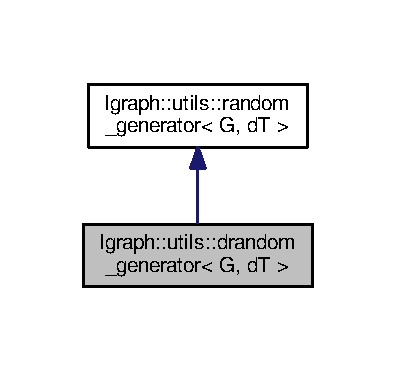
\includegraphics[width=190pt]{classlgraph_1_1utils_1_1drandom__generator__inherit__graph}
\end{center}
\end{figure}


Collaboration diagram for lgraph\-:\-:utils\-:\-:drandom\-\_\-generator$<$ G, d\-T $>$\-:\nopagebreak
\begin{figure}[H]
\begin{center}
\leavevmode
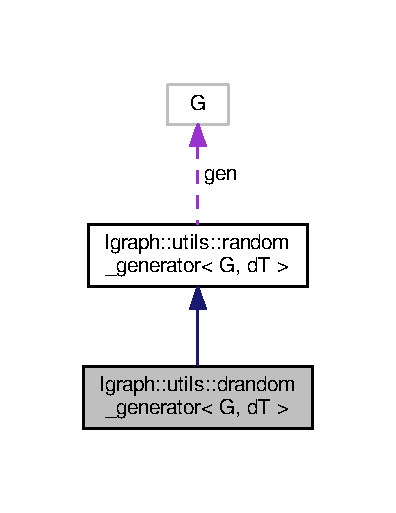
\includegraphics[width=190pt]{classlgraph_1_1utils_1_1drandom__generator__coll__graph}
\end{center}
\end{figure}
\subsection*{Public Member Functions}
\begin{DoxyCompactItemize}
\item 
\hypertarget{classlgraph_1_1utils_1_1drandom__generator_a3029c9cb8b6e73b0e0f0ca5fbc33c6ea}{\hyperlink{classlgraph_1_1utils_1_1drandom__generator_a3029c9cb8b6e73b0e0f0ca5fbc33c6ea}{drandom\-\_\-generator} ()}\label{classlgraph_1_1utils_1_1drandom__generator_a3029c9cb8b6e73b0e0f0ca5fbc33c6ea}

\begin{DoxyCompactList}\small\item\em Constructor. \end{DoxyCompactList}\item 
\hypertarget{classlgraph_1_1utils_1_1drandom__generator_a09711a23359454bf60cefb2e0be64a0a}{\hyperlink{classlgraph_1_1utils_1_1drandom__generator_a09711a23359454bf60cefb2e0be64a0a}{$\sim$drandom\-\_\-generator} ()}\label{classlgraph_1_1utils_1_1drandom__generator_a09711a23359454bf60cefb2e0be64a0a}

\begin{DoxyCompactList}\small\item\em Destructor. \end{DoxyCompactList}\item 
void \hyperlink{classlgraph_1_1utils_1_1drandom__generator_a38c5b5c981d635aac32f632a0f4a0092}{init\-\_\-uniform} (d\-T a, d\-T b)
\begin{DoxyCompactList}\small\item\em Initialise the uniform distribution. \end{DoxyCompactList}\item 
void \hyperlink{classlgraph_1_1utils_1_1drandom__generator_acae17810176a40fdfd8a4a260892361e}{init\-\_\-binomial} (d\-T a, double p)
\begin{DoxyCompactList}\small\item\em Initialise the binomial distribution. \end{DoxyCompactList}\item 
\hypertarget{classlgraph_1_1utils_1_1drandom__generator_a7735e31610688246957518795169bae3}{d\-T \hyperlink{classlgraph_1_1utils_1_1drandom__generator_a7735e31610688246957518795169bae3}{get\-\_\-uniform} ()}\label{classlgraph_1_1utils_1_1drandom__generator_a7735e31610688246957518795169bae3}

\begin{DoxyCompactList}\small\item\em Compute a pseudo-\/random number uniformly at random. \end{DoxyCompactList}\item 
\hypertarget{classlgraph_1_1utils_1_1drandom__generator_ac6062b1bbf3ed3a45bdab7474f466b7f}{d\-T \hyperlink{classlgraph_1_1utils_1_1drandom__generator_ac6062b1bbf3ed3a45bdab7474f466b7f}{get\-\_\-binomial} ()}\label{classlgraph_1_1utils_1_1drandom__generator_ac6062b1bbf3ed3a45bdab7474f466b7f}

\begin{DoxyCompactList}\small\item\em Compute a pseudo-\/random binomal number. \end{DoxyCompactList}\item 
\hypertarget{classlgraph_1_1utils_1_1random__generator_a4eb6998070eecb59bd89dca92d8a509c}{virtual void \hyperlink{classlgraph_1_1utils_1_1random__generator_a4eb6998070eecb59bd89dca92d8a509c}{seed\-\_\-random\-\_\-engine} ()}\label{classlgraph_1_1utils_1_1random__generator_a4eb6998070eecb59bd89dca92d8a509c}

\begin{DoxyCompactList}\small\item\em Initialises the random engine. \end{DoxyCompactList}\end{DoxyCompactItemize}
\subsection*{Protected Attributes}
\begin{DoxyCompactItemize}
\item 
\hypertarget{classlgraph_1_1utils_1_1random__generator_a18353876b4c2d3a18aee454b5750a0a0}{G \hyperlink{classlgraph_1_1utils_1_1random__generator_a18353876b4c2d3a18aee454b5750a0a0}{gen}}\label{classlgraph_1_1utils_1_1random__generator_a18353876b4c2d3a18aee454b5750a0a0}

\begin{DoxyCompactList}\small\item\em Random engine. \end{DoxyCompactList}\end{DoxyCompactItemize}
\subsection*{Private Attributes}
\begin{DoxyCompactItemize}
\item 
\hypertarget{classlgraph_1_1utils_1_1drandom__generator_a995de3b90cefebba7aa0d93a7900bebb}{std\-::uniform\-\_\-int\-\_\-distribution\\*
$<$ d\-T $>$ $\ast$ \hyperlink{classlgraph_1_1utils_1_1drandom__generator_a995de3b90cefebba7aa0d93a7900bebb}{U}}\label{classlgraph_1_1utils_1_1drandom__generator_a995de3b90cefebba7aa0d93a7900bebb}

\begin{DoxyCompactList}\small\item\em Object to generate integer numbers uniformly at random. \end{DoxyCompactList}\item 
\hypertarget{classlgraph_1_1utils_1_1drandom__generator_abf2a3acb2bdee25e7fef80d465d69c97}{std\-::binomial\-\_\-distribution$<$ d\-T $>$ $\ast$ \hyperlink{classlgraph_1_1utils_1_1drandom__generator_abf2a3acb2bdee25e7fef80d465d69c97}{B}}\label{classlgraph_1_1utils_1_1drandom__generator_abf2a3acb2bdee25e7fef80d465d69c97}

\begin{DoxyCompactList}\small\item\em Object to generate the numbers following a binomial distribution. \end{DoxyCompactList}\end{DoxyCompactItemize}


\subsection{Detailed Description}
\subsubsection*{template$<$class G = std\-::default\-\_\-random\-\_\-engine, typename d\-T = size\-\_\-t$>$class lgraph\-::utils\-::drandom\-\_\-generator$<$ G, d\-T $>$}

Discrete pseudo-\/\-Random Number Generator (D\-R\-N\-G). 

Class that generates discrete numbers in both uniform and binomial distributions.


\begin{DoxyParams}{Parameters}
{\em G} & The random engine used to generate the numbers. \\
\hline
{\em T} & The type of the numbers generated (int, char, unsigned int, ...). \\
\hline
\end{DoxyParams}


\subsection{Member Function Documentation}
\hypertarget{classlgraph_1_1utils_1_1drandom__generator_acae17810176a40fdfd8a4a260892361e}{\index{lgraph\-::utils\-::drandom\-\_\-generator@{lgraph\-::utils\-::drandom\-\_\-generator}!init\-\_\-binomial@{init\-\_\-binomial}}
\index{init\-\_\-binomial@{init\-\_\-binomial}!lgraph::utils::drandom_generator@{lgraph\-::utils\-::drandom\-\_\-generator}}
\subsubsection[{init\-\_\-binomial}]{\setlength{\rightskip}{0pt plus 5cm}template$<$class G , typename d\-T $>$ void {\bf lgraph\-::utils\-::drandom\-\_\-generator}$<$ G, d\-T $>$\-::init\-\_\-binomial (
\begin{DoxyParamCaption}
\item[{d\-T}]{n, }
\item[{double}]{p}
\end{DoxyParamCaption}
)\hspace{0.3cm}{\ttfamily [virtual]}}}\label{classlgraph_1_1utils_1_1drandom__generator_acae17810176a40fdfd8a4a260892361e}


Initialise the binomial distribution. 


\begin{DoxyParams}{Parameters}
{\em n} & Number of independent experiments of the distribution. \\
\hline
{\em p} & Probability of success of each experiment. \\
\hline
\end{DoxyParams}


Implements \hyperlink{classlgraph_1_1utils_1_1random__generator_a71976e6ecbbd49de85ac270085832df1}{lgraph\-::utils\-::random\-\_\-generator$<$ G, d\-T $>$}.

\hypertarget{classlgraph_1_1utils_1_1drandom__generator_a38c5b5c981d635aac32f632a0f4a0092}{\index{lgraph\-::utils\-::drandom\-\_\-generator@{lgraph\-::utils\-::drandom\-\_\-generator}!init\-\_\-uniform@{init\-\_\-uniform}}
\index{init\-\_\-uniform@{init\-\_\-uniform}!lgraph::utils::drandom_generator@{lgraph\-::utils\-::drandom\-\_\-generator}}
\subsubsection[{init\-\_\-uniform}]{\setlength{\rightskip}{0pt plus 5cm}template$<$class G , typename d\-T $>$ void {\bf lgraph\-::utils\-::drandom\-\_\-generator}$<$ G, d\-T $>$\-::init\-\_\-uniform (
\begin{DoxyParamCaption}
\item[{d\-T}]{a, }
\item[{d\-T}]{b}
\end{DoxyParamCaption}
)\hspace{0.3cm}{\ttfamily [virtual]}}}\label{classlgraph_1_1utils_1_1drandom__generator_a38c5b5c981d635aac32f632a0f4a0092}


Initialise the uniform distribution. 


\begin{DoxyParams}{Parameters}
{\em a} & Lower bound of the interval of the distribution. \\
\hline
{\em b} & Upper bound of the interval of the distribution. \\
\hline
\end{DoxyParams}


Implements \hyperlink{classlgraph_1_1utils_1_1random__generator_a129da597bed5b08e9c7e5a3ddce4287c}{lgraph\-::utils\-::random\-\_\-generator$<$ G, d\-T $>$}.



The documentation for this class was generated from the following files\-:\begin{DoxyCompactItemize}
\item 
lgraph/utils/random\-\_\-generator.\-hpp\item 
lgraph/utils/drandom\-\_\-generator.\-cpp\end{DoxyCompactItemize}

\hypertarget{classlgraph_1_1utils_1_1logger}{}\section{lgraph\+:\+:utils\+:\+:logger$<$ out\+\_\+stream $>$ Class Template Reference}
\label{classlgraph_1_1utils_1_1logger}\index{lgraph\+::utils\+::logger$<$ out\+\_\+stream $>$@{lgraph\+::utils\+::logger$<$ out\+\_\+stream $>$}}


Class for message display.  




{\ttfamily \#include $<$logger.\+hpp$>$}

\subsection*{Public Member Functions}
\begin{DoxyCompactItemize}
\item 
out\+\_\+stream \& \hyperlink{classlgraph_1_1utils_1_1logger_aa5458017ffc7b65faff47f55a056c2c5}{log} ()
\begin{DoxyCompactList}\small\item\em Returns the stream to output information to. \end{DoxyCompactList}\item 
\mbox{\Hypertarget{classlgraph_1_1utils_1_1logger_ad1e8cb0e83b2d9a90cbcd57e59fcca32}\label{classlgraph_1_1utils_1_1logger_ad1e8cb0e83b2d9a90cbcd57e59fcca32}} 
\hyperlink{classlgraph_1_1utils_1_1logger_ad1e8cb0e83b2d9a90cbcd57e59fcca32}{logger} (const \hyperlink{classlgraph_1_1utils_1_1logger}{logger} \&L)=delete
\begin{DoxyCompactList}\small\item\em Deleted copy-\/constructor. \end{DoxyCompactList}\item 
\mbox{\Hypertarget{classlgraph_1_1utils_1_1logger_aabccbc9d1ef5c0eb431eca9f08e4af12}\label{classlgraph_1_1utils_1_1logger_aabccbc9d1ef5c0eb431eca9f08e4af12}} 
void \hyperlink{classlgraph_1_1utils_1_1logger_aabccbc9d1ef5c0eb431eca9f08e4af12}{operator=} (const \hyperlink{classlgraph_1_1utils_1_1logger}{logger} \&L)=delete
\begin{DoxyCompactList}\small\item\em Deleted assignation operator. \end{DoxyCompactList}\end{DoxyCompactItemize}
\subsection*{Static Public Member Functions}
\begin{DoxyCompactItemize}
\item 
static \hyperlink{classlgraph_1_1utils_1_1logger}{logger} \& \hyperlink{classlgraph_1_1utils_1_1logger_af9d53836a2c37c72a08cf14f7e071abb}{get\+\_\+logger} (const std\+::string \&o=\char`\"{}log.\+txt\char`\"{})
\begin{DoxyCompactList}\small\item\em Returns the only instance of this class. \end{DoxyCompactList}\end{DoxyCompactItemize}
\subsection*{Private Member Functions}
\begin{DoxyCompactItemize}
\item 
\hyperlink{classlgraph_1_1utils_1_1logger_ace2028a4b282e3cb6593f6f62fee2f2b}{logger} ()
\begin{DoxyCompactList}\small\item\em Empty constructor. \end{DoxyCompactList}\end{DoxyCompactItemize}
\subsection*{Private Attributes}
\begin{DoxyCompactItemize}
\item 
\mbox{\Hypertarget{classlgraph_1_1utils_1_1logger_aafc1693e642fc967fed16b78d5cd8a5f}\label{classlgraph_1_1utils_1_1logger_aafc1693e642fc967fed16b78d5cd8a5f}} 
out\+\_\+stream \hyperlink{classlgraph_1_1utils_1_1logger_aafc1693e642fc967fed16b78d5cd8a5f}{fout}
\begin{DoxyCompactList}\small\item\em The stream object to output the strings to. \end{DoxyCompactList}\item 
\mbox{\Hypertarget{classlgraph_1_1utils_1_1logger_a2e159433db285ccfc8120a4aa4ea7481}\label{classlgraph_1_1utils_1_1logger_a2e159433db285ccfc8120a4aa4ea7481}} 
bool \hyperlink{classlgraph_1_1utils_1_1logger_a2e159433db285ccfc8120a4aa4ea7481}{opened}
\begin{DoxyCompactList}\small\item\em In case of an stream to a file, is it opened?. \end{DoxyCompactList}\end{DoxyCompactItemize}


\subsection{Detailed Description}
\subsubsection*{template$<$class out\+\_\+stream = std\+::ofstream$>$\newline
class lgraph\+::utils\+::logger$<$ out\+\_\+stream $>$}

Class for message display. 

Singleton class to centralise the displaying of messages either to the standard or error output, or to a file. For example, during development it is useful to have \char`\"{}couts\char`\"{} to display the values of variables, to show the progress of algorithms, ...

Once the development is complete, one may want to get rid of these couts by deleting them. This may be a bad idea since bugs may be discovered later in the development of the project. To avoid their deletion/comment-\/out, the logger can be used in the following way\+: \begin{DoxyVerb}logger<cout_stream>& LOG = logger<cout_stream>::get_logger();   // declare the object\n
LOG.log() << "message 1" << std::endl;  // Use it   \n
LOG.log() << "message 2" << std::endl;              \n\n
\end{DoxyVerb}


Once we are not interested in displaying messages anymore, change the declaration of the object to\+: \begin{DoxyVerb}utils::logger<utils::null_stream>& LOG =
    utils::logger<utils::null_stream>::get_logger();
\end{DoxyVerb}


The other calls displaying \char`\"{}message $\ast$\char`\"{} will have no effect. There is only one instance of this class for a \hyperlink{classlgraph_1_1utils_1_1cout__stream}{cout\+\_\+stream}, one for a \hyperlink{classlgraph_1_1utils_1_1cerr__stream}{cerr\+\_\+stream}, one for a \hyperlink{classlgraph_1_1utils_1_1null__stream}{null\+\_\+stream}, and another for a stream to a file.


\begin{DoxyParams}{Parameters}
{\em out\+\_\+stream} & The ofstream type or the \hyperlink{classlgraph_1_1utils_1_1null__stream}{null\+\_\+stream}. \hyperlink{classlgraph_1_1utils_1_1cout__stream}{cout\+\_\+stream}, \hyperlink{classlgraph_1_1utils_1_1cerr__stream}{cerr\+\_\+stream}. \\
\hline
\end{DoxyParams}


\subsection{Constructor \& Destructor Documentation}
\mbox{\Hypertarget{classlgraph_1_1utils_1_1logger_ace2028a4b282e3cb6593f6f62fee2f2b}\label{classlgraph_1_1utils_1_1logger_ace2028a4b282e3cb6593f6f62fee2f2b}} 
\index{lgraph\+::utils\+::logger@{lgraph\+::utils\+::logger}!logger@{logger}}
\index{logger@{logger}!lgraph\+::utils\+::logger@{lgraph\+::utils\+::logger}}
\subsubsection{\texorpdfstring{logger()}{logger()}}
{\footnotesize\ttfamily template$<$class out\+\_\+stream = std\+::ofstream$>$ \\
\hyperlink{classlgraph_1_1utils_1_1logger}{lgraph\+::utils\+::logger}$<$ out\+\_\+stream $>$\+::\hyperlink{classlgraph_1_1utils_1_1logger}{logger} (\begin{DoxyParamCaption}{ }\end{DoxyParamCaption})\hspace{0.3cm}{\ttfamily [inline]}, {\ttfamily [private]}}



Empty constructor. 

Made private to make this class a singleton. 

\subsection{Member Function Documentation}
\mbox{\Hypertarget{classlgraph_1_1utils_1_1logger_af9d53836a2c37c72a08cf14f7e071abb}\label{classlgraph_1_1utils_1_1logger_af9d53836a2c37c72a08cf14f7e071abb}} 
\index{lgraph\+::utils\+::logger@{lgraph\+::utils\+::logger}!get\+\_\+logger@{get\+\_\+logger}}
\index{get\+\_\+logger@{get\+\_\+logger}!lgraph\+::utils\+::logger@{lgraph\+::utils\+::logger}}
\subsubsection{\texorpdfstring{get\+\_\+logger()}{get\_logger()}}
{\footnotesize\ttfamily template$<$class out\+\_\+stream = std\+::ofstream$>$ \\
static \hyperlink{classlgraph_1_1utils_1_1logger}{logger}\& \hyperlink{classlgraph_1_1utils_1_1logger}{lgraph\+::utils\+::logger}$<$ out\+\_\+stream $>$\+::get\+\_\+logger (\begin{DoxyParamCaption}\item[{const std\+::string \&}]{o = {\ttfamily \char`\"{}log.txt\char`\"{}} }\end{DoxyParamCaption})\hspace{0.3cm}{\ttfamily [inline]}, {\ttfamily [static]}}



Returns the only instance of this class. 


\begin{DoxyParams}{Parameters}
{\em o} & In case of using a stream to a file (ofstream), indicate the name of the file. \\
\hline
\end{DoxyParams}
\begin{DoxyReturn}{Returns}
Returns the only instance of this class of the indicated type in the template parameter. 
\end{DoxyReturn}
\mbox{\Hypertarget{classlgraph_1_1utils_1_1logger_aa5458017ffc7b65faff47f55a056c2c5}\label{classlgraph_1_1utils_1_1logger_aa5458017ffc7b65faff47f55a056c2c5}} 
\index{lgraph\+::utils\+::logger@{lgraph\+::utils\+::logger}!log@{log}}
\index{log@{log}!lgraph\+::utils\+::logger@{lgraph\+::utils\+::logger}}
\subsubsection{\texorpdfstring{log()}{log()}}
{\footnotesize\ttfamily template$<$class out\+\_\+stream = std\+::ofstream$>$ \\
out\+\_\+stream\& \hyperlink{classlgraph_1_1utils_1_1logger}{lgraph\+::utils\+::logger}$<$ out\+\_\+stream $>$\+::log (\begin{DoxyParamCaption}{ }\end{DoxyParamCaption})\hspace{0.3cm}{\ttfamily [inline]}}



Returns the stream to output information to. 

This works exactly like the \textquotesingle{}cout\textquotesingle{} and \textquotesingle{}cerr\textquotesingle{} ostream classes. All objects passed to this using \textquotesingle{}$<$$<$\textquotesingle{} must implement this operator. 

The documentation for this class was generated from the following file\+:\begin{DoxyCompactItemize}
\item 
lgraph/utils/logger.\+hpp\end{DoxyCompactItemize}

\hypertarget{classlgraph_1_1utils_1_1node__path}{}\section{lgraph\+:\+:utils\+:\+:node\+\_\+path$<$ T $>$ Class Template Reference}
\label{classlgraph_1_1utils_1_1node__path}\index{lgraph\+::utils\+::node\+\_\+path$<$ T $>$@{lgraph\+::utils\+::node\+\_\+path$<$ T $>$}}


A path through a grpah seen as a list of nodes.  




{\ttfamily \#include $<$node\+\_\+path.\+hpp$>$}

\subsection*{Public Member Functions}
\begin{DoxyCompactItemize}
\item 
\hyperlink{classlgraph_1_1utils_1_1node__path_a480b23324e337e2a895c33a444e04e72}{node\+\_\+path} ()\hypertarget{classlgraph_1_1utils_1_1node__path_a480b23324e337e2a895c33a444e04e72}{}\label{classlgraph_1_1utils_1_1node__path_a480b23324e337e2a895c33a444e04e72}

\begin{DoxyCompactList}\small\item\em Empty constructor. \end{DoxyCompactList}\item 
\hyperlink{classlgraph_1_1utils_1_1node__path_a3d2fbb25f163d99a643c8a3d61c5749f}{node\+\_\+path} (\hyperlink{namespacelgraph_1_1utils_ab9c6b34241f0b68372c55f34c460e863}{node} n)
\begin{DoxyCompactList}\small\item\em Initialise a path starting at node {\itshape n}. \end{DoxyCompactList}\item 
void \hyperlink{classlgraph_1_1utils_1_1node__path_a5d652d22c59d4e538de4d483de4fef7d}{empty} ()
\begin{DoxyCompactList}\small\item\em Empties this path. \end{DoxyCompactList}\item 
\hyperlink{namespacelgraph_1_1utils_ab9c6b34241f0b68372c55f34c460e863}{node} \hyperlink{classlgraph_1_1utils_1_1node__path_ad182d2c41a3833585841deed101f203d}{operator\mbox{[}$\,$\mbox{]}} (size\+\_\+t i) const 
\begin{DoxyCompactList}\small\item\em Acces the {\itshape i-\/th} node of this path. \end{DoxyCompactList}\item 
\hyperlink{namespacelgraph_1_1utils_ab9c6b34241f0b68372c55f34c460e863}{node} \& \hyperlink{classlgraph_1_1utils_1_1node__path_aa2191c4a123c0b7dbf55ae7f407045bf}{operator\mbox{[}$\,$\mbox{]}} (size\+\_\+t i)
\begin{DoxyCompactList}\small\item\em Acces the {\itshape i-\/th} node of this path. \end{DoxyCompactList}\item 
bool \hyperlink{classlgraph_1_1utils_1_1node__path_ad0be002c0ecfafcd29f2332f4fae07a3}{operator$<$} (const \hyperlink{classlgraph_1_1utils_1_1node__path}{node\+\_\+path}$<$ T $>$ \&p) const \hypertarget{classlgraph_1_1utils_1_1node__path_ad0be002c0ecfafcd29f2332f4fae07a3}{}\label{classlgraph_1_1utils_1_1node__path_ad0be002c0ecfafcd29f2332f4fae07a3}

\begin{DoxyCompactList}\small\item\em Compares two nodes using only their length. \end{DoxyCompactList}\item 
bool \hyperlink{classlgraph_1_1utils_1_1node__path_a50387915894923c9e999c157da6e4812}{operator$>$} (const \hyperlink{classlgraph_1_1utils_1_1node__path}{node\+\_\+path}$<$ T $>$ \&p) const \hypertarget{classlgraph_1_1utils_1_1node__path_a50387915894923c9e999c157da6e4812}{}\label{classlgraph_1_1utils_1_1node__path_a50387915894923c9e999c157da6e4812}

\begin{DoxyCompactList}\small\item\em Compares two nodes using only their length. \end{DoxyCompactList}\item 
\hyperlink{classlgraph_1_1utils_1_1node__path}{node\+\_\+path}$<$ T $>$ \& \hyperlink{classlgraph_1_1utils_1_1node__path_a394176d986b6f7c3f3f51978dde52172}{operator=} (const \hyperlink{classlgraph_1_1utils_1_1node__path}{node\+\_\+path}$<$ T $>$ \&np)\hypertarget{classlgraph_1_1utils_1_1node__path_a394176d986b6f7c3f3f51978dde52172}{}\label{classlgraph_1_1utils_1_1node__path_a394176d986b6f7c3f3f51978dde52172}

\begin{DoxyCompactList}\small\item\em Assigns the contents of {\itshape np} to this path. \end{DoxyCompactList}\item 
void \hyperlink{classlgraph_1_1utils_1_1node__path_a0c5109bd203149e8e99b9f0b3790fb8f}{concatenate} (const \hyperlink{classlgraph_1_1utils_1_1node__path}{node\+\_\+path} \&p)
\begin{DoxyCompactList}\small\item\em Concatenates the two paths. \end{DoxyCompactList}\item 
void \hyperlink{classlgraph_1_1utils_1_1node__path_afdbba890740d013c8fcca7081461b240}{add\+\_\+node} (\hyperlink{namespacelgraph_1_1utils_ab9c6b34241f0b68372c55f34c460e863}{node} u)
\begin{DoxyCompactList}\small\item\em Adds a node to the path. \end{DoxyCompactList}\item 
void \hyperlink{classlgraph_1_1utils_1_1node__path_a400ebcaf58927f3a22a5fbb91f1fe3a6}{add\+\_\+length} (const T \&l)
\begin{DoxyCompactList}\small\item\em Accumulates to the current length of the the path the value l. \end{DoxyCompactList}\item 
void \hyperlink{classlgraph_1_1utils_1_1node__path_a0b64dae8a7d12cbf85452e697e5cde34}{set\+\_\+length} (const T \&l)
\begin{DoxyCompactList}\small\item\em Sets the current length of the the path the value l. \end{DoxyCompactList}\item 
void \hyperlink{classlgraph_1_1utils_1_1node__path_ae7e803a3945812e692804bfbcb85423c}{reverse} ()\hypertarget{classlgraph_1_1utils_1_1node__path_ae7e803a3945812e692804bfbcb85423c}{}\label{classlgraph_1_1utils_1_1node__path_ae7e803a3945812e692804bfbcb85423c}

\begin{DoxyCompactList}\small\item\em Reverses the order of the nodes of this path. \end{DoxyCompactList}\item 
void \hyperlink{classlgraph_1_1utils_1_1node__path_a3fa7b2c4aca2bc9edfdabf8f7c6c1434}{delete\+\_\+last} ()
\begin{DoxyCompactList}\small\item\em Deletes the last node of this path. \end{DoxyCompactList}\item 
size\+\_\+t \hyperlink{classlgraph_1_1utils_1_1node__path_a8f2480fc8be847b42513c40e86fb3df4}{size} () const 
\begin{DoxyCompactList}\small\item\em Returns the number of nodes in this path. \end{DoxyCompactList}\item 
T \hyperlink{classlgraph_1_1utils_1_1node__path_a9e620f75025d76beecded0d771acbca6}{get\+\_\+length} () const 
\begin{DoxyCompactList}\small\item\em Returns the length of this path. \end{DoxyCompactList}\item 
\hyperlink{namespacelgraph_1_1utils_ab9c6b34241f0b68372c55f34c460e863}{node} \hyperlink{classlgraph_1_1utils_1_1node__path_a74b2525643c2804885a94d7e6fa50ee2}{last\+\_\+node} () const \hypertarget{classlgraph_1_1utils_1_1node__path_a74b2525643c2804885a94d7e6fa50ee2}{}\label{classlgraph_1_1utils_1_1node__path_a74b2525643c2804885a94d7e6fa50ee2}

\begin{DoxyCompactList}\small\item\em Return the last node of this path. \end{DoxyCompactList}\item 
const vector$<$ \hyperlink{namespacelgraph_1_1utils_ab9c6b34241f0b68372c55f34c460e863}{node} $>$ \& \hyperlink{classlgraph_1_1utils_1_1node__path_a9c5553326f2ffaaf6727b90b1363222a}{get\+\_\+nodes} () const \hypertarget{classlgraph_1_1utils_1_1node__path_a9c5553326f2ffaaf6727b90b1363222a}{}\label{classlgraph_1_1utils_1_1node__path_a9c5553326f2ffaaf6727b90b1363222a}

\begin{DoxyCompactList}\small\item\em Returns a constant reference to the list of nodes. \end{DoxyCompactList}\item 
string \hyperlink{classlgraph_1_1utils_1_1node__path_ab71d9301f2d5c93083a1ef875fa6c3ab}{to\+\_\+string} () const 
\begin{DoxyCompactList}\small\item\em Formats this path into a string with a plain format. \end{DoxyCompactList}\item 
void \hyperlink{classlgraph_1_1utils_1_1node__path_aa35035a582b89ccb21e7c18a86c3ada2}{to\+\_\+string} (string \&s) const 
\begin{DoxyCompactList}\small\item\em Formats this path into a string with a plain format. \end{DoxyCompactList}\end{DoxyCompactItemize}
\subsection*{Private Attributes}
\begin{DoxyCompactItemize}
\item 
vector$<$ \hyperlink{namespacelgraph_1_1utils_ab9c6b34241f0b68372c55f34c460e863}{node} $>$ \hyperlink{classlgraph_1_1utils_1_1node__path_af0067294d0390cef2c11ece4b080257c}{nodes}\hypertarget{classlgraph_1_1utils_1_1node__path_af0067294d0390cef2c11ece4b080257c}{}\label{classlgraph_1_1utils_1_1node__path_af0067294d0390cef2c11ece4b080257c}

\begin{DoxyCompactList}\small\item\em The list of nodes of this path. \end{DoxyCompactList}\item 
T \hyperlink{classlgraph_1_1utils_1_1node__path_a43d91c7647402a07b896d74cb4a7a783}{path\+\_\+length}
\begin{DoxyCompactList}\small\item\em The total weight of this path. \end{DoxyCompactList}\end{DoxyCompactItemize}
\subsection*{Friends}
\begin{DoxyCompactItemize}
\item 
ostream \& \hyperlink{classlgraph_1_1utils_1_1node__path_aaa2ab8603e9a2ab44dd473a2a4a722b0}{operator$<$$<$} (ostream \&os, const \hyperlink{classlgraph_1_1utils_1_1node__path}{node\+\_\+path}$<$ T $>$ \&np)
\begin{DoxyCompactList}\small\item\em Outputs this path on a {\itshape ostream} object. \end{DoxyCompactList}\end{DoxyCompactItemize}


\subsection{Detailed Description}
\subsubsection*{template$<$class T = \+\_\+new\+\_\+$>$\\*
class lgraph\+::utils\+::node\+\_\+path$<$ T $>$}

A path through a grpah seen as a list of nodes. 

It simply stores a list of nodes in which every pair of consecutive nodes form an edge in a graph. If all consecutive pairs of nodes make a path in a graph {\itshape G} then this object stores a path within {\itshape G}.

It also stores the length of the path, that is, the sum of all the edges in this path.


\begin{DoxyParams}{Parameters}
{\em T} & The type used for the length. It must support comparisons and the C++\textquotesingle{}s output operator $<$$<$. \\
\hline
\end{DoxyParams}


\subsection{Constructor \& Destructor Documentation}
\index{lgraph\+::utils\+::node\+\_\+path@{lgraph\+::utils\+::node\+\_\+path}!node\+\_\+path@{node\+\_\+path}}
\index{node\+\_\+path@{node\+\_\+path}!lgraph\+::utils\+::node\+\_\+path@{lgraph\+::utils\+::node\+\_\+path}}
\subsubsection[{\texorpdfstring{node\+\_\+path(node n)}{node_path(node n)}}]{\setlength{\rightskip}{0pt plus 5cm}template$<$class T $>$ {\bf lgraph\+::utils\+::node\+\_\+path}$<$ T $>$\+::{\bf node\+\_\+path} (
\begin{DoxyParamCaption}
\item[{{\bf node}}]{n}
\end{DoxyParamCaption}
)}\hypertarget{classlgraph_1_1utils_1_1node__path_a3d2fbb25f163d99a643c8a3d61c5749f}{}\label{classlgraph_1_1utils_1_1node__path_a3d2fbb25f163d99a643c8a3d61c5749f}


Initialise a path starting at node {\itshape n}. 


\begin{DoxyParams}{Parameters}
{\em n} & The first node of this path. \\
\hline
\end{DoxyParams}
\begin{DoxyPrecond}{Precondition}
{\itshape n} $>$= 0 
\end{DoxyPrecond}


\subsection{Member Function Documentation}
\index{lgraph\+::utils\+::node\+\_\+path@{lgraph\+::utils\+::node\+\_\+path}!add\+\_\+length@{add\+\_\+length}}
\index{add\+\_\+length@{add\+\_\+length}!lgraph\+::utils\+::node\+\_\+path@{lgraph\+::utils\+::node\+\_\+path}}
\subsubsection[{\texorpdfstring{add\+\_\+length(const T \&l)}{add_length(const T &l)}}]{\setlength{\rightskip}{0pt plus 5cm}template$<$class T $>$ void {\bf lgraph\+::utils\+::node\+\_\+path}$<$ T $>$\+::add\+\_\+length (
\begin{DoxyParamCaption}
\item[{const T \&}]{l}
\end{DoxyParamCaption}
)}\hypertarget{classlgraph_1_1utils_1_1node__path_a400ebcaf58927f3a22a5fbb91f1fe3a6}{}\label{classlgraph_1_1utils_1_1node__path_a400ebcaf58927f3a22a5fbb91f1fe3a6}


Accumulates to the current length of the the path the value l. 


\begin{DoxyParams}{Parameters}
{\em l} & The value to be accumulated to \hyperlink{classlgraph_1_1utils_1_1node__path_a43d91c7647402a07b896d74cb4a7a783}{path\+\_\+length} \\
\hline
\end{DoxyParams}
\index{lgraph\+::utils\+::node\+\_\+path@{lgraph\+::utils\+::node\+\_\+path}!add\+\_\+node@{add\+\_\+node}}
\index{add\+\_\+node@{add\+\_\+node}!lgraph\+::utils\+::node\+\_\+path@{lgraph\+::utils\+::node\+\_\+path}}
\subsubsection[{\texorpdfstring{add\+\_\+node(node u)}{add_node(node u)}}]{\setlength{\rightskip}{0pt plus 5cm}template$<$class T $>$ void {\bf lgraph\+::utils\+::node\+\_\+path}$<$ T $>$\+::add\+\_\+node (
\begin{DoxyParamCaption}
\item[{{\bf node}}]{u}
\end{DoxyParamCaption}
)}\hypertarget{classlgraph_1_1utils_1_1node__path_afdbba890740d013c8fcca7081461b240}{}\label{classlgraph_1_1utils_1_1node__path_afdbba890740d013c8fcca7081461b240}


Adds a node to the path. 

The new node is added at the back of \hyperlink{classlgraph_1_1utils_1_1node__path_af0067294d0390cef2c11ece4b080257c}{nodes} 
\begin{DoxyParams}{Parameters}
{\em u} & The node\textquotesingle{}s index \\
\hline
\end{DoxyParams}
\begin{DoxyPrecond}{Precondition}
u $>$= 0 
\end{DoxyPrecond}
\begin{DoxyPostcond}{Postcondition}
The length remains unchanged 
\end{DoxyPostcond}
\index{lgraph\+::utils\+::node\+\_\+path@{lgraph\+::utils\+::node\+\_\+path}!concatenate@{concatenate}}
\index{concatenate@{concatenate}!lgraph\+::utils\+::node\+\_\+path@{lgraph\+::utils\+::node\+\_\+path}}
\subsubsection[{\texorpdfstring{concatenate(const node\+\_\+path \&p)}{concatenate(const node_path &p)}}]{\setlength{\rightskip}{0pt plus 5cm}template$<$class T $>$ void {\bf lgraph\+::utils\+::node\+\_\+path}$<$ T $>$\+::concatenate (
\begin{DoxyParamCaption}
\item[{const {\bf node\+\_\+path}$<$ T $>$ \&}]{p}
\end{DoxyParamCaption}
)}\hypertarget{classlgraph_1_1utils_1_1node__path_a0c5109bd203149e8e99b9f0b3790fb8f}{}\label{classlgraph_1_1utils_1_1node__path_a0c5109bd203149e8e99b9f0b3790fb8f}


Concatenates the two paths. 

Adds at the end of this path all nodes in {\itshape p} except for the first. The length of {\itshape p} will be accumulated to this path\textquotesingle{}s length.


\begin{DoxyParams}{Parameters}
{\em p} & The path to be appended to this. \\
\hline
\end{DoxyParams}
\begin{DoxyPrecond}{Precondition}
This path\textquotesingle{}s last node and the first node of p must be the same. 
\end{DoxyPrecond}
\index{lgraph\+::utils\+::node\+\_\+path@{lgraph\+::utils\+::node\+\_\+path}!delete\+\_\+last@{delete\+\_\+last}}
\index{delete\+\_\+last@{delete\+\_\+last}!lgraph\+::utils\+::node\+\_\+path@{lgraph\+::utils\+::node\+\_\+path}}
\subsubsection[{\texorpdfstring{delete\+\_\+last()}{delete_last()}}]{\setlength{\rightskip}{0pt plus 5cm}template$<$class T $>$ void {\bf lgraph\+::utils\+::node\+\_\+path}$<$ T $>$\+::delete\+\_\+last (
\begin{DoxyParamCaption}
{}
\end{DoxyParamCaption}
)}\hypertarget{classlgraph_1_1utils_1_1node__path_a3fa7b2c4aca2bc9edfdabf8f7c6c1434}{}\label{classlgraph_1_1utils_1_1node__path_a3fa7b2c4aca2bc9edfdabf8f7c6c1434}


Deletes the last node of this path. 

\begin{DoxyPostcond}{Postcondition}
The length remains unchanged 
\end{DoxyPostcond}
\index{lgraph\+::utils\+::node\+\_\+path@{lgraph\+::utils\+::node\+\_\+path}!empty@{empty}}
\index{empty@{empty}!lgraph\+::utils\+::node\+\_\+path@{lgraph\+::utils\+::node\+\_\+path}}
\subsubsection[{\texorpdfstring{empty()}{empty()}}]{\setlength{\rightskip}{0pt plus 5cm}template$<$class T $>$ void {\bf lgraph\+::utils\+::node\+\_\+path}$<$ T $>$\+::empty (
\begin{DoxyParamCaption}
{}
\end{DoxyParamCaption}
)}\hypertarget{classlgraph_1_1utils_1_1node__path_a5d652d22c59d4e538de4d483de4fef7d}{}\label{classlgraph_1_1utils_1_1node__path_a5d652d22c59d4e538de4d483de4fef7d}


Empties this path. 

Frees the memory occupied by the currently existing nodes. Sets \hyperlink{classlgraph_1_1utils_1_1node__path_a43d91c7647402a07b896d74cb4a7a783}{path\+\_\+length} to 0. \index{lgraph\+::utils\+::node\+\_\+path@{lgraph\+::utils\+::node\+\_\+path}!get\+\_\+length@{get\+\_\+length}}
\index{get\+\_\+length@{get\+\_\+length}!lgraph\+::utils\+::node\+\_\+path@{lgraph\+::utils\+::node\+\_\+path}}
\subsubsection[{\texorpdfstring{get\+\_\+length() const }{get_length() const }}]{\setlength{\rightskip}{0pt plus 5cm}template$<$class T $>$ T {\bf lgraph\+::utils\+::node\+\_\+path}$<$ T $>$\+::get\+\_\+length (
\begin{DoxyParamCaption}
{}
\end{DoxyParamCaption}
) const}\hypertarget{classlgraph_1_1utils_1_1node__path_a9e620f75025d76beecded0d771acbca6}{}\label{classlgraph_1_1utils_1_1node__path_a9e620f75025d76beecded0d771acbca6}


Returns the length of this path. 

\begin{DoxyReturn}{Returns}
Returns the value \hyperlink{classlgraph_1_1utils_1_1node__path_a43d91c7647402a07b896d74cb4a7a783}{path\+\_\+length} 
\end{DoxyReturn}
\index{lgraph\+::utils\+::node\+\_\+path@{lgraph\+::utils\+::node\+\_\+path}!operator\mbox{[}$\,$\mbox{]}@{operator[]}}
\index{operator\mbox{[}$\,$\mbox{]}@{operator[]}!lgraph\+::utils\+::node\+\_\+path@{lgraph\+::utils\+::node\+\_\+path}}
\subsubsection[{\texorpdfstring{operator[](size\+\_\+t i) const }{operator[](size_t i) const }}]{\setlength{\rightskip}{0pt plus 5cm}template$<$class T $>$ {\bf node} {\bf lgraph\+::utils\+::node\+\_\+path}$<$ T $>$\+::operator\mbox{[}$\,$\mbox{]} (
\begin{DoxyParamCaption}
\item[{size\+\_\+t}]{i}
\end{DoxyParamCaption}
) const}\hypertarget{classlgraph_1_1utils_1_1node__path_ad182d2c41a3833585841deed101f203d}{}\label{classlgraph_1_1utils_1_1node__path_ad182d2c41a3833585841deed101f203d}


Acces the {\itshape i-\/th} node of this path. 


\begin{DoxyParams}{Parameters}
{\em i} & Index of the list \\
\hline
\end{DoxyParams}
\begin{DoxyReturn}{Returns}
A copy of the node at the i-\/th position 
\end{DoxyReturn}
\begin{DoxyPrecond}{Precondition}
0 $<$= {\itshape i} $<$ {\itshape n} with {\itshape n} the amount of nodes in this path 
\end{DoxyPrecond}
\index{lgraph\+::utils\+::node\+\_\+path@{lgraph\+::utils\+::node\+\_\+path}!operator\mbox{[}$\,$\mbox{]}@{operator[]}}
\index{operator\mbox{[}$\,$\mbox{]}@{operator[]}!lgraph\+::utils\+::node\+\_\+path@{lgraph\+::utils\+::node\+\_\+path}}
\subsubsection[{\texorpdfstring{operator[](size\+\_\+t i)}{operator[](size_t i)}}]{\setlength{\rightskip}{0pt plus 5cm}template$<$class T $>$ {\bf node} \& {\bf lgraph\+::utils\+::node\+\_\+path}$<$ T $>$\+::operator\mbox{[}$\,$\mbox{]} (
\begin{DoxyParamCaption}
\item[{size\+\_\+t}]{i}
\end{DoxyParamCaption}
)}\hypertarget{classlgraph_1_1utils_1_1node__path_aa2191c4a123c0b7dbf55ae7f407045bf}{}\label{classlgraph_1_1utils_1_1node__path_aa2191c4a123c0b7dbf55ae7f407045bf}


Acces the {\itshape i-\/th} node of this path. 


\begin{DoxyParams}{Parameters}
{\em i} & Index of the list \\
\hline
\end{DoxyParams}
\begin{DoxyReturn}{Returns}
A reference to the node at the i-\/th position 
\end{DoxyReturn}
\begin{DoxyPrecond}{Precondition}
0 $<$= {\itshape i} $<$ {\itshape n} with {\itshape n} the amount of nodes in this path 
\end{DoxyPrecond}
\index{lgraph\+::utils\+::node\+\_\+path@{lgraph\+::utils\+::node\+\_\+path}!set\+\_\+length@{set\+\_\+length}}
\index{set\+\_\+length@{set\+\_\+length}!lgraph\+::utils\+::node\+\_\+path@{lgraph\+::utils\+::node\+\_\+path}}
\subsubsection[{\texorpdfstring{set\+\_\+length(const T \&l)}{set_length(const T &l)}}]{\setlength{\rightskip}{0pt plus 5cm}template$<$class T $>$ void {\bf lgraph\+::utils\+::node\+\_\+path}$<$ T $>$\+::set\+\_\+length (
\begin{DoxyParamCaption}
\item[{const T \&}]{l}
\end{DoxyParamCaption}
)}\hypertarget{classlgraph_1_1utils_1_1node__path_a0b64dae8a7d12cbf85452e697e5cde34}{}\label{classlgraph_1_1utils_1_1node__path_a0b64dae8a7d12cbf85452e697e5cde34}


Sets the current length of the the path the value l. 


\begin{DoxyParams}{Parameters}
{\em l} & The value that will replace the current value of \hyperlink{classlgraph_1_1utils_1_1node__path_a43d91c7647402a07b896d74cb4a7a783}{path\+\_\+length} \\
\hline
\end{DoxyParams}
\index{lgraph\+::utils\+::node\+\_\+path@{lgraph\+::utils\+::node\+\_\+path}!size@{size}}
\index{size@{size}!lgraph\+::utils\+::node\+\_\+path@{lgraph\+::utils\+::node\+\_\+path}}
\subsubsection[{\texorpdfstring{size() const }{size() const }}]{\setlength{\rightskip}{0pt plus 5cm}template$<$class T $>$ size\+\_\+t {\bf lgraph\+::utils\+::node\+\_\+path}$<$ T $>$\+::size (
\begin{DoxyParamCaption}
{}
\end{DoxyParamCaption}
) const}\hypertarget{classlgraph_1_1utils_1_1node__path_a8f2480fc8be847b42513c40e86fb3df4}{}\label{classlgraph_1_1utils_1_1node__path_a8f2480fc8be847b42513c40e86fb3df4}


Returns the number of nodes in this path. 

\begin{DoxyReturn}{Returns}
Returns the size of \hyperlink{classlgraph_1_1utils_1_1node__path_af0067294d0390cef2c11ece4b080257c}{nodes} 
\end{DoxyReturn}
\index{lgraph\+::utils\+::node\+\_\+path@{lgraph\+::utils\+::node\+\_\+path}!to\+\_\+string@{to\+\_\+string}}
\index{to\+\_\+string@{to\+\_\+string}!lgraph\+::utils\+::node\+\_\+path@{lgraph\+::utils\+::node\+\_\+path}}
\subsubsection[{\texorpdfstring{to\+\_\+string() const }{to_string() const }}]{\setlength{\rightskip}{0pt plus 5cm}template$<$class T $>$ string {\bf lgraph\+::utils\+::node\+\_\+path}$<$ T $>$\+::to\+\_\+string (
\begin{DoxyParamCaption}
{}
\end{DoxyParamCaption}
) const}\hypertarget{classlgraph_1_1utils_1_1node__path_ab71d9301f2d5c93083a1ef875fa6c3ab}{}\label{classlgraph_1_1utils_1_1node__path_ab71d9301f2d5c93083a1ef875fa6c3ab}


Formats this path into a string with a plain format. 

\begin{DoxyReturn}{Returns}
Returns this path as a list of indexes, each representing a node. 
\end{DoxyReturn}
\index{lgraph\+::utils\+::node\+\_\+path@{lgraph\+::utils\+::node\+\_\+path}!to\+\_\+string@{to\+\_\+string}}
\index{to\+\_\+string@{to\+\_\+string}!lgraph\+::utils\+::node\+\_\+path@{lgraph\+::utils\+::node\+\_\+path}}
\subsubsection[{\texorpdfstring{to\+\_\+string(string \&s) const }{to_string(string &s) const }}]{\setlength{\rightskip}{0pt plus 5cm}template$<$class T $>$ void {\bf lgraph\+::utils\+::node\+\_\+path}$<$ T $>$\+::to\+\_\+string (
\begin{DoxyParamCaption}
\item[{string \&}]{s}
\end{DoxyParamCaption}
) const}\hypertarget{classlgraph_1_1utils_1_1node__path_aa35035a582b89ccb21e7c18a86c3ada2}{}\label{classlgraph_1_1utils_1_1node__path_aa35035a582b89ccb21e7c18a86c3ada2}


Formats this path into a string with a plain format. 


\begin{DoxyParams}[1]{Parameters}
\mbox{\tt out}  & {\em s} & Stores this path as a list of indexes, each representing a node. \\
\hline
\end{DoxyParams}


\subsection{Friends And Related Function Documentation}
\index{lgraph\+::utils\+::node\+\_\+path@{lgraph\+::utils\+::node\+\_\+path}!operator$<$$<$@{operator$<$$<$}}
\index{operator$<$$<$@{operator$<$$<$}!lgraph\+::utils\+::node\+\_\+path@{lgraph\+::utils\+::node\+\_\+path}}
\subsubsection[{\texorpdfstring{operator$<$$<$}{operator<<}}]{\setlength{\rightskip}{0pt plus 5cm}template$<$class T = \+\_\+new\+\_\+$>$ ostream\& operator$<$$<$ (
\begin{DoxyParamCaption}
\item[{ostream \&}]{os, }
\item[{const {\bf node\+\_\+path}$<$ T $>$ \&}]{np}
\end{DoxyParamCaption}
)\hspace{0.3cm}{\ttfamily [friend]}}\hypertarget{classlgraph_1_1utils_1_1node__path_aaa2ab8603e9a2ab44dd473a2a4a722b0}{}\label{classlgraph_1_1utils_1_1node__path_aaa2ab8603e9a2ab44dd473a2a4a722b0}


Outputs this path on a {\itshape ostream} object. 

The format is a space-\/separated list of indices (one for each node) followed by \textquotesingle{}-\/$>$\textquotesingle{} and this path\textquotesingle{}s length. 

\subsection{Member Data Documentation}
\index{lgraph\+::utils\+::node\+\_\+path@{lgraph\+::utils\+::node\+\_\+path}!path\+\_\+length@{path\+\_\+length}}
\index{path\+\_\+length@{path\+\_\+length}!lgraph\+::utils\+::node\+\_\+path@{lgraph\+::utils\+::node\+\_\+path}}
\subsubsection[{\texorpdfstring{path\+\_\+length}{path_length}}]{\setlength{\rightskip}{0pt plus 5cm}template$<$class T = \+\_\+new\+\_\+$>$ T {\bf lgraph\+::utils\+::node\+\_\+path}$<$ T $>$\+::path\+\_\+length\hspace{0.3cm}{\ttfamily [private]}}\hypertarget{classlgraph_1_1utils_1_1node__path_a43d91c7647402a07b896d74cb4a7a783}{}\label{classlgraph_1_1utils_1_1node__path_a43d91c7647402a07b896d74cb4a7a783}


The total weight of this path. 

If \textquotesingle{}p\textquotesingle{} is the path as a list of edges, then \textquotesingle{}path\+\_\+length\textquotesingle{} equals the sum of weights of all edges in \textquotesingle{}p\textquotesingle{}. 

The documentation for this class was generated from the following files\+:\begin{DoxyCompactItemize}
\item 
lgraph/data\+\_\+structures/node\+\_\+path.\+hpp\item 
lgraph/data\+\_\+structures/node\+\_\+path.\+cpp\end{DoxyCompactItemize}

\hypertarget{classlgraph_1_1utils_1_1null__stream}{}\section{lgraph\+:\+:utils\+:\+:null\+\_\+stream Class Reference}
\label{classlgraph_1_1utils_1_1null__stream}\index{lgraph\+::utils\+::null\+\_\+stream@{lgraph\+::utils\+::null\+\_\+stream}}


A class for a null stream.  




{\ttfamily \#include $<$logger.\+hpp$>$}

\subsection*{Public Types}
\begin{DoxyCompactItemize}
\item 
typedef std\+::basic\+\_\+ostream$<$ char, std\+::char\+\_\+traits$<$ char $>$ $>$ \hyperlink{classlgraph_1_1utils_1_1null__stream_ae3f818cbd342cb6da9f15677252da938}{cout\+\_\+type}\hypertarget{classlgraph_1_1utils_1_1null__stream_ae3f818cbd342cb6da9f15677252da938}{}\label{classlgraph_1_1utils_1_1null__stream_ae3f818cbd342cb6da9f15677252da938}

\begin{DoxyCompactList}\small\item\em This is the type of std\+::cout. \end{DoxyCompactList}\item 
typedef \hyperlink{classlgraph_1_1utils_1_1null__stream_ae3f818cbd342cb6da9f15677252da938}{cout\+\_\+type} \&($\ast$ \hyperlink{classlgraph_1_1utils_1_1null__stream_ada7be393792a0f7b90452c981a279d08}{standard\+\_\+endl}) (\hyperlink{classlgraph_1_1utils_1_1null__stream_ae3f818cbd342cb6da9f15677252da938}{cout\+\_\+type} \&)\hypertarget{classlgraph_1_1utils_1_1null__stream_ada7be393792a0f7b90452c981a279d08}{}\label{classlgraph_1_1utils_1_1null__stream_ada7be393792a0f7b90452c981a279d08}

\begin{DoxyCompactList}\small\item\em This is the function signature of std\+::endl. \end{DoxyCompactList}\end{DoxyCompactItemize}
\subsection*{Public Member Functions}
\begin{DoxyCompactItemize}
\item 
void \hyperlink{classlgraph_1_1utils_1_1null__stream_a4b1d2687e779efef7d4995bcede83448}{open} (const char $\ast$, const std\+::ios\+\_\+base\+::openmode \&)\hypertarget{classlgraph_1_1utils_1_1null__stream_a4b1d2687e779efef7d4995bcede83448}{}\label{classlgraph_1_1utils_1_1null__stream_a4b1d2687e779efef7d4995bcede83448}

\begin{DoxyCompactList}\small\item\em Open an empty stream for null messages. \end{DoxyCompactList}\item 
\hyperlink{classlgraph_1_1utils_1_1null__stream}{null\+\_\+stream} \& \hyperlink{classlgraph_1_1utils_1_1null__stream_a6dd6b8cde39e03fe63eb2feef89ebc11}{operator$<$$<$} (const \hyperlink{classlgraph_1_1utils_1_1null__stream_ada7be393792a0f7b90452c981a279d08}{standard\+\_\+endl} \&)\hypertarget{classlgraph_1_1utils_1_1null__stream_a6dd6b8cde39e03fe63eb2feef89ebc11}{}\label{classlgraph_1_1utils_1_1null__stream_a6dd6b8cde39e03fe63eb2feef89ebc11}

\begin{DoxyCompactList}\small\item\em Define an operator$<$$<$ to take in std\+::endl. \end{DoxyCompactList}\item 
{\footnotesize template$<$class t\+\_\+printable $>$ }\\\hyperlink{classlgraph_1_1utils_1_1null__stream}{null\+\_\+stream} \& \hyperlink{classlgraph_1_1utils_1_1null__stream_a633f62bff5dd6e4973674d2f109732cf}{operator$<$$<$} (const t\+\_\+printable \&)\hypertarget{classlgraph_1_1utils_1_1null__stream_a633f62bff5dd6e4973674d2f109732cf}{}\label{classlgraph_1_1utils_1_1null__stream_a633f62bff5dd6e4973674d2f109732cf}

\begin{DoxyCompactList}\small\item\em operator$<$$<$ for any printable type \end{DoxyCompactList}\end{DoxyCompactItemize}


\subsection{Detailed Description}
A class for a null stream. 

The operator \textquotesingle{}$<$$<$\textquotesingle{} for any suitable type does not have any effect on it (nothing is displayed). The \textquotesingle{}endl\textquotesingle{} modifier is also redefined to have no effect on the stream. 

The documentation for this class was generated from the following file\+:\begin{DoxyCompactItemize}
\item 
lgraph/utils/logger.\+hpp\end{DoxyCompactItemize}

\hypertarget{classlgraph_1_1utils_1_1random__generator}{}\section{lgraph\+:\+:utils\+:\+:random\+\_\+generator$<$ G, T $>$ Class Template Reference}
\label{classlgraph_1_1utils_1_1random__generator}\index{lgraph\+::utils\+::random\+\_\+generator$<$ G, T $>$@{lgraph\+::utils\+::random\+\_\+generator$<$ G, T $>$}}


Abstract pseudo-\/\+Random Number Generator (A\+R\+NG).  




{\ttfamily \#include $<$random\+\_\+generator.\+hpp$>$}



Collaboration diagram for lgraph\+:\+:utils\+:\+:random\+\_\+generator$<$ G, T $>$\+:\nopagebreak
\begin{figure}[H]
\begin{center}
\leavevmode
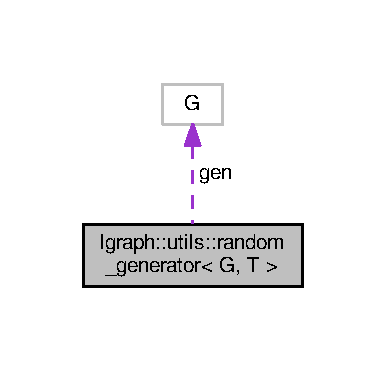
\includegraphics[width=185pt]{classlgraph_1_1utils_1_1random__generator__coll__graph}
\end{center}
\end{figure}
\subsection*{Public Member Functions}
\begin{DoxyCompactItemize}
\item 
\mbox{\Hypertarget{classlgraph_1_1utils_1_1random__generator_af4f4ba363f6f72d3ded2dba9e97079bb}\label{classlgraph_1_1utils_1_1random__generator_af4f4ba363f6f72d3ded2dba9e97079bb}} 
\hyperlink{classlgraph_1_1utils_1_1random__generator_af4f4ba363f6f72d3ded2dba9e97079bb}{random\+\_\+generator} ()
\begin{DoxyCompactList}\small\item\em Class constructor. \end{DoxyCompactList}\item 
\mbox{\Hypertarget{classlgraph_1_1utils_1_1random__generator_a87783727d9e3a109bc3ed0631edad69b}\label{classlgraph_1_1utils_1_1random__generator_a87783727d9e3a109bc3ed0631edad69b}} 
virtual \hyperlink{classlgraph_1_1utils_1_1random__generator_a87783727d9e3a109bc3ed0631edad69b}{$\sim$random\+\_\+generator} ()
\begin{DoxyCompactList}\small\item\em Class destructor. \end{DoxyCompactList}\item 
\mbox{\Hypertarget{classlgraph_1_1utils_1_1random__generator_a4eb6998070eecb59bd89dca92d8a509c}\label{classlgraph_1_1utils_1_1random__generator_a4eb6998070eecb59bd89dca92d8a509c}} 
virtual void \hyperlink{classlgraph_1_1utils_1_1random__generator_a4eb6998070eecb59bd89dca92d8a509c}{seed\+\_\+random\+\_\+engine} ()
\begin{DoxyCompactList}\small\item\em Initialises the random engine. \end{DoxyCompactList}\item 
virtual void \hyperlink{classlgraph_1_1utils_1_1random__generator_a129da597bed5b08e9c7e5a3ddce4287c}{init\+\_\+uniform} (T a, T b)=0
\begin{DoxyCompactList}\small\item\em Initialise the uniform distribution. \end{DoxyCompactList}\item 
virtual void \hyperlink{classlgraph_1_1utils_1_1random__generator_a71976e6ecbbd49de85ac270085832df1}{init\+\_\+binomial} (T n, double p)=0
\begin{DoxyCompactList}\small\item\em Initialise the binomial distribution. \end{DoxyCompactList}\item 
\mbox{\Hypertarget{classlgraph_1_1utils_1_1random__generator_ac18bd12c8baf8a7cbe6ef9be072c95cf}\label{classlgraph_1_1utils_1_1random__generator_ac18bd12c8baf8a7cbe6ef9be072c95cf}} 
virtual T \hyperlink{classlgraph_1_1utils_1_1random__generator_ac18bd12c8baf8a7cbe6ef9be072c95cf}{get\+\_\+uniform} ()=0
\begin{DoxyCompactList}\small\item\em Compute a pseudo-\/random number uniformly at random. \end{DoxyCompactList}\item 
\mbox{\Hypertarget{classlgraph_1_1utils_1_1random__generator_a721da14c38e38d28559e8c617e0bdde2}\label{classlgraph_1_1utils_1_1random__generator_a721da14c38e38d28559e8c617e0bdde2}} 
virtual T \hyperlink{classlgraph_1_1utils_1_1random__generator_a721da14c38e38d28559e8c617e0bdde2}{get\+\_\+binomial} ()=0
\begin{DoxyCompactList}\small\item\em Compute a pseudo-\/random binomal number. \end{DoxyCompactList}\end{DoxyCompactItemize}
\subsection*{Protected Attributes}
\begin{DoxyCompactItemize}
\item 
\mbox{\Hypertarget{classlgraph_1_1utils_1_1random__generator_a18353876b4c2d3a18aee454b5750a0a0}\label{classlgraph_1_1utils_1_1random__generator_a18353876b4c2d3a18aee454b5750a0a0}} 
G \hyperlink{classlgraph_1_1utils_1_1random__generator_a18353876b4c2d3a18aee454b5750a0a0}{gen}
\begin{DoxyCompactList}\small\item\em Random engine. \end{DoxyCompactList}\end{DoxyCompactItemize}


\subsection{Detailed Description}
\subsubsection*{template$<$class G, typename T$>$\newline
class lgraph\+::utils\+::random\+\_\+generator$<$ G, T $>$}

Abstract pseudo-\/\+Random Number Generator (A\+R\+NG). 

Interface for random number generators using the C++11 header $<$random$>$.

Seed the random engine calling method \hyperlink{classlgraph_1_1utils_1_1random__generator_a4eb6998070eecb59bd89dca92d8a509c}{seed\+\_\+random\+\_\+engine()}.

Initialise whatever distribution is needed with the appropriate method\+:
\begin{DoxyItemize}
\item \hyperlink{classlgraph_1_1utils_1_1random__generator_a129da597bed5b08e9c7e5a3ddce4287c}{init\+\_\+uniform(\+T a, T b)} to generate numbers following the distribution U\mbox{[}a,b\mbox{]}, where U denotes the uniform distribution.
\item \hyperlink{classlgraph_1_1utils_1_1random__generator_a71976e6ecbbd49de85ac270085832df1}{init\+\_\+binomial(\+T n, double p)} to generate numbers following the distribution B(n,p), where B denotes the binomial distribution.
\end{DoxyItemize}


\begin{DoxyParams}{Parameters}
{\em G} & The random engine used to generate the numbers \\
\hline
{\em T} & The type of the numbers generated (its type depends on the subclass that will implement the interface) \\
\hline
\end{DoxyParams}


\subsection{Member Function Documentation}
\mbox{\Hypertarget{classlgraph_1_1utils_1_1random__generator_a71976e6ecbbd49de85ac270085832df1}\label{classlgraph_1_1utils_1_1random__generator_a71976e6ecbbd49de85ac270085832df1}} 
\index{lgraph\+::utils\+::random\+\_\+generator@{lgraph\+::utils\+::random\+\_\+generator}!init\+\_\+binomial@{init\+\_\+binomial}}
\index{init\+\_\+binomial@{init\+\_\+binomial}!lgraph\+::utils\+::random\+\_\+generator@{lgraph\+::utils\+::random\+\_\+generator}}
\subsubsection{\texorpdfstring{init\+\_\+binomial()}{init\_binomial()}}
{\footnotesize\ttfamily template$<$class G, typename T$>$ \\
virtual void \hyperlink{classlgraph_1_1utils_1_1random__generator}{lgraph\+::utils\+::random\+\_\+generator}$<$ G, T $>$\+::init\+\_\+binomial (\begin{DoxyParamCaption}\item[{T}]{n,  }\item[{double}]{p }\end{DoxyParamCaption})\hspace{0.3cm}{\ttfamily [pure virtual]}}



Initialise the binomial distribution. 


\begin{DoxyParams}{Parameters}
{\em n} & Number of independent experiments of the distribution. \\
\hline
{\em p} & Probability of success of each experiment. \\
\hline
\end{DoxyParams}


Implemented in \hyperlink{classlgraph_1_1utils_1_1crandom__generator_a4d7042cb0862c3b8b4792890e6c5388c}{lgraph\+::utils\+::crandom\+\_\+generator$<$ G, c\+T $>$}, and \hyperlink{classlgraph_1_1utils_1_1drandom__generator_acae17810176a40fdfd8a4a260892361e}{lgraph\+::utils\+::drandom\+\_\+generator$<$ G, d\+T $>$}.

\mbox{\Hypertarget{classlgraph_1_1utils_1_1random__generator_a129da597bed5b08e9c7e5a3ddce4287c}\label{classlgraph_1_1utils_1_1random__generator_a129da597bed5b08e9c7e5a3ddce4287c}} 
\index{lgraph\+::utils\+::random\+\_\+generator@{lgraph\+::utils\+::random\+\_\+generator}!init\+\_\+uniform@{init\+\_\+uniform}}
\index{init\+\_\+uniform@{init\+\_\+uniform}!lgraph\+::utils\+::random\+\_\+generator@{lgraph\+::utils\+::random\+\_\+generator}}
\subsubsection{\texorpdfstring{init\+\_\+uniform()}{init\_uniform()}}
{\footnotesize\ttfamily template$<$class G, typename T$>$ \\
virtual void \hyperlink{classlgraph_1_1utils_1_1random__generator}{lgraph\+::utils\+::random\+\_\+generator}$<$ G, T $>$\+::init\+\_\+uniform (\begin{DoxyParamCaption}\item[{T}]{a,  }\item[{T}]{b }\end{DoxyParamCaption})\hspace{0.3cm}{\ttfamily [pure virtual]}}



Initialise the uniform distribution. 


\begin{DoxyParams}{Parameters}
{\em a} & Lower bound of the interval of the distribution. \\
\hline
{\em b} & Upper bound of the interval of the distribution. \\
\hline
\end{DoxyParams}


Implemented in \hyperlink{classlgraph_1_1utils_1_1crandom__generator_addfa5951276296b2a164e5dc482728ce}{lgraph\+::utils\+::crandom\+\_\+generator$<$ G, c\+T $>$}, and \hyperlink{classlgraph_1_1utils_1_1drandom__generator_a38c5b5c981d635aac32f632a0f4a0092}{lgraph\+::utils\+::drandom\+\_\+generator$<$ G, d\+T $>$}.



The documentation for this class was generated from the following files\+:\begin{DoxyCompactItemize}
\item 
lgraph/utils/random\+\_\+generator.\+hpp\item 
lgraph/utils/random\+\_\+generator.\+cpp\end{DoxyCompactItemize}

\hypertarget{classlgraph_1_1utils_1_1static__bitset}{}\section{lgraph\+:\+:utils\+:\+:static\+\_\+bitset Class Reference}
\label{classlgraph_1_1utils_1_1static__bitset}\index{lgraph\+::utils\+::static\+\_\+bitset@{lgraph\+::utils\+::static\+\_\+bitset}}


Bitset class.  




{\ttfamily \#include $<$static\+\_\+bitset.\+hpp$>$}

\subsection*{Public Member Functions}
\begin{DoxyCompactItemize}
\item 
\mbox{\Hypertarget{classlgraph_1_1utils_1_1static__bitset_a6bd7edf22c70684b97eed197bb8fcda5}\label{classlgraph_1_1utils_1_1static__bitset_a6bd7edf22c70684b97eed197bb8fcda5}} 
\hyperlink{classlgraph_1_1utils_1_1static__bitset_a6bd7edf22c70684b97eed197bb8fcda5}{static\+\_\+bitset} ()
\begin{DoxyCompactList}\small\item\em Empty constructor. \end{DoxyCompactList}\item 
\mbox{\Hypertarget{classlgraph_1_1utils_1_1static__bitset_ad8aaa938472eb7fcdc3ac1b3270600f6}\label{classlgraph_1_1utils_1_1static__bitset_ad8aaa938472eb7fcdc3ac1b3270600f6}} 
\hyperlink{classlgraph_1_1utils_1_1static__bitset_ad8aaa938472eb7fcdc3ac1b3270600f6}{static\+\_\+bitset} (const std\+::string \&bs)
\begin{DoxyCompactList}\small\item\em Construct a bitset from a string of zeros and ones. \hyperlink{classlgraph_1_1utils_1_1static__bitset_a56d277fc22bbf71a27fca530a133c9bd}{bytes}\mbox{[}i\mbox{]} = {\itshape bs}\mbox{[}i\mbox{]}. \end{DoxyCompactList}\item 
\mbox{\Hypertarget{classlgraph_1_1utils_1_1static__bitset_a98921bd3c2ef416c5270045c63eb84a1}\label{classlgraph_1_1utils_1_1static__bitset_a98921bd3c2ef416c5270045c63eb84a1}} 
\hyperlink{classlgraph_1_1utils_1_1static__bitset_a98921bd3c2ef416c5270045c63eb84a1}{static\+\_\+bitset} (const std\+::vector$<$ bool $>$ \&bits)
\begin{DoxyCompactList}\small\item\em Construct a bitset from a list of Boolean values. \hyperlink{classlgraph_1_1utils_1_1static__bitset_a56d277fc22bbf71a27fca530a133c9bd}{bytes}\mbox{[}i\mbox{]} = {\itshape bits}\mbox{[}i\mbox{]}. \end{DoxyCompactList}\item 
\mbox{\Hypertarget{classlgraph_1_1utils_1_1static__bitset_a683aec1377830f07c5d5f53f969be569}\label{classlgraph_1_1utils_1_1static__bitset_a683aec1377830f07c5d5f53f969be569}} 
\hyperlink{classlgraph_1_1utils_1_1static__bitset_a683aec1377830f07c5d5f53f969be569}{static\+\_\+bitset} (const \hyperlink{classlgraph_1_1utils_1_1static__bitset}{static\+\_\+bitset} \&bs)
\begin{DoxyCompactList}\small\item\em Copy-\/constructor. \end{DoxyCompactList}\item 
\mbox{\Hypertarget{classlgraph_1_1utils_1_1static__bitset_aabbb46d8283fffa38b39204b204999be}\label{classlgraph_1_1utils_1_1static__bitset_aabbb46d8283fffa38b39204b204999be}} 
\hyperlink{classlgraph_1_1utils_1_1static__bitset_aabbb46d8283fffa38b39204b204999be}{$\sim$static\+\_\+bitset} ()
\begin{DoxyCompactList}\small\item\em Destructor. \end{DoxyCompactList}\item 
void \hyperlink{classlgraph_1_1utils_1_1static__bitset_afad1ede9e08c9d59b641150d2203edca}{init} (size\+\_\+t \hyperlink{classlgraph_1_1utils_1_1static__bitset_aebc02986838d70f13d3c10f390d11211}{n\+\_\+bits})
\begin{DoxyCompactList}\small\item\em Initialise the bitset with {\itshape n\+\_\+bits} bits. \end{DoxyCompactList}\item 
void \hyperlink{classlgraph_1_1utils_1_1static__bitset_a706ac4c15ed634b9087582cacc107acc}{init\+\_\+set} (size\+\_\+t \hyperlink{classlgraph_1_1utils_1_1static__bitset_aebc02986838d70f13d3c10f390d11211}{n\+\_\+bits})
\begin{DoxyCompactList}\small\item\em Initialise the bitset with {\itshape n\+\_\+bits} bits all of them set to 1. \end{DoxyCompactList}\item 
void \hyperlink{classlgraph_1_1utils_1_1static__bitset_a6fb4d66f266593fe9c65451bf6212591}{init\+\_\+unset} (size\+\_\+t \hyperlink{classlgraph_1_1utils_1_1static__bitset_aebc02986838d70f13d3c10f390d11211}{n\+\_\+bits})
\begin{DoxyCompactList}\small\item\em Initialise the bitset with {\itshape n\+\_\+bits} bits all of them set to 0. \end{DoxyCompactList}\item 
void \hyperlink{classlgraph_1_1utils_1_1static__bitset_ab94cca3ec07c19d17a205eb486fc6cdd}{init\+\_\+01} (const std\+::string \&zerones)
\begin{DoxyCompactList}\small\item\em Initialise the bitset from a string of zeros and ones. \end{DoxyCompactList}\item 
void \hyperlink{classlgraph_1_1utils_1_1static__bitset_a223b698841c841d517155f5cdcc1c9a4}{init\+\_\+01} (const std\+::vector$<$ bool $>$ \&bits)
\begin{DoxyCompactList}\small\item\em Initialise the bitset from a list of Boolean values. \end{DoxyCompactList}\item 
void \hyperlink{classlgraph_1_1utils_1_1static__bitset_a00b39bf2552cbab68a9d5ee7f430e59d}{init\+\_\+bytes} (const std\+::vector$<$ char $>$ \&\hyperlink{classlgraph_1_1utils_1_1static__bitset_a56d277fc22bbf71a27fca530a133c9bd}{bytes})
\begin{DoxyCompactList}\small\item\em Initialise the bitset from a string of bytes. \end{DoxyCompactList}\item 
void \hyperlink{classlgraph_1_1utils_1_1static__bitset_a8fe9cefb9a05d30b1586810c6ccda923}{init\+\_\+bytes} (const std\+::string \&\hyperlink{classlgraph_1_1utils_1_1static__bitset_a56d277fc22bbf71a27fca530a133c9bd}{bytes})
\begin{DoxyCompactList}\small\item\em Initialise the bitset from a string of bytes. \end{DoxyCompactList}\item 
void \hyperlink{classlgraph_1_1utils_1_1static__bitset_a6013f8230ae37554328dfe0884d89c71}{clear} ()
\begin{DoxyCompactList}\small\item\em Frees the memory occupied by the bitset. \end{DoxyCompactList}\item 
\hyperlink{classlgraph_1_1utils_1_1static__bitset}{static\+\_\+bitset} \& \hyperlink{classlgraph_1_1utils_1_1static__bitset_a3215c8066fffcd8eed871914d42c40b8}{operator=} (const \hyperlink{classlgraph_1_1utils_1_1static__bitset}{static\+\_\+bitset} \&bs)
\begin{DoxyCompactList}\small\item\em Asigns the contents of {\itshape bs} to this bitset. \end{DoxyCompactList}\item 
\mbox{\Hypertarget{classlgraph_1_1utils_1_1static__bitset_ac992361d2d5264ce8382f2e44ee939fb}\label{classlgraph_1_1utils_1_1static__bitset_ac992361d2d5264ce8382f2e44ee939fb}} 
bool \hyperlink{classlgraph_1_1utils_1_1static__bitset_ac992361d2d5264ce8382f2e44ee939fb}{operator\mbox{[}$\,$\mbox{]}} (size\+\_\+t i) const
\begin{DoxyCompactList}\small\item\em Returns the value of the i-\/th bit. \end{DoxyCompactList}\item 
\hyperlink{classlgraph_1_1utils_1_1static__bitset}{static\+\_\+bitset} \hyperlink{classlgraph_1_1utils_1_1static__bitset_a633df0acba7afd646bbbef1acd85ca49}{operator$<$=} (const \hyperlink{classlgraph_1_1utils_1_1static__bitset}{static\+\_\+bitset} \&bs) const
\begin{DoxyCompactList}\small\item\em Inclusion operator. \end{DoxyCompactList}\item 
\hyperlink{classlgraph_1_1utils_1_1static__bitset}{static\+\_\+bitset} \hyperlink{classlgraph_1_1utils_1_1static__bitset_a8bb49442a841f4a899f355fb278a9468}{operator$\sim$} () const
\begin{DoxyCompactList}\small\item\em Unary not operator. \end{DoxyCompactList}\item 
\hyperlink{classlgraph_1_1utils_1_1static__bitset}{static\+\_\+bitset} \hyperlink{classlgraph_1_1utils_1_1static__bitset_ab7ab47c906e9e08a61a48bb935594e90}{operator-\/} (const \hyperlink{classlgraph_1_1utils_1_1static__bitset}{static\+\_\+bitset} \&bs) const
\begin{DoxyCompactList}\small\item\em Bitset difference operator. \end{DoxyCompactList}\item 
\hyperlink{classlgraph_1_1utils_1_1static__bitset}{static\+\_\+bitset} \hyperlink{classlgraph_1_1utils_1_1static__bitset_ade4bed9c986a5f328535c133bfa8eee7}{operator \&} (const \hyperlink{classlgraph_1_1utils_1_1static__bitset}{static\+\_\+bitset} \&bs) const
\begin{DoxyCompactList}\small\item\em Bitwise {\itshape and} operator. \end{DoxyCompactList}\item 
\hyperlink{classlgraph_1_1utils_1_1static__bitset}{static\+\_\+bitset} \hyperlink{classlgraph_1_1utils_1_1static__bitset_a8b0ee09d74157739ac96995b6a07b29f}{operator$\vert$} (const \hyperlink{classlgraph_1_1utils_1_1static__bitset}{static\+\_\+bitset} \&bs) const
\begin{DoxyCompactList}\small\item\em Bitwise {\itshape or} operator. \end{DoxyCompactList}\item 
\hyperlink{classlgraph_1_1utils_1_1static__bitset}{static\+\_\+bitset} \hyperlink{classlgraph_1_1utils_1_1static__bitset_a5d4ca0e342e0b0094f20925a62b2068d}{operator$^\wedge$} (const \hyperlink{classlgraph_1_1utils_1_1static__bitset}{static\+\_\+bitset} \&bs) const
\begin{DoxyCompactList}\small\item\em Bitwise {\itshape exclusive-\/or} operator. \end{DoxyCompactList}\item 
\hyperlink{classlgraph_1_1utils_1_1static__bitset}{static\+\_\+bitset} \hyperlink{classlgraph_1_1utils_1_1static__bitset_a901bec6cc27e6b521d33b8658223e1ea}{operator==} (const \hyperlink{classlgraph_1_1utils_1_1static__bitset}{static\+\_\+bitset} \&bs) const
\begin{DoxyCompactList}\small\item\em Bitwise {\itshape equality} operator. \end{DoxyCompactList}\item 
\hyperlink{classlgraph_1_1utils_1_1static__bitset}{static\+\_\+bitset} \& \hyperlink{classlgraph_1_1utils_1_1static__bitset_af4f4a29642e50b6efa406d5f772a0e69}{operator-\/=} (const \hyperlink{classlgraph_1_1utils_1_1static__bitset}{static\+\_\+bitset} \&bs)
\begin{DoxyCompactList}\small\item\em Bitwise {\itshape difference} operator. \end{DoxyCompactList}\item 
\hyperlink{classlgraph_1_1utils_1_1static__bitset}{static\+\_\+bitset} \& \hyperlink{classlgraph_1_1utils_1_1static__bitset_a9be18d0f80ce54324ff6a37e86e125d7}{operator \&=} (const \hyperlink{classlgraph_1_1utils_1_1static__bitset}{static\+\_\+bitset} \&bs)
\begin{DoxyCompactList}\small\item\em Bitwise {\itshape and} operator. \end{DoxyCompactList}\item 
\hyperlink{classlgraph_1_1utils_1_1static__bitset}{static\+\_\+bitset} \& \hyperlink{classlgraph_1_1utils_1_1static__bitset_a62330084392296754cfc5e525d99cab2}{operator$\vert$=} (const \hyperlink{classlgraph_1_1utils_1_1static__bitset}{static\+\_\+bitset} \&bs)
\begin{DoxyCompactList}\small\item\em Bitwise {\itshape or} operator. \end{DoxyCompactList}\item 
\hyperlink{classlgraph_1_1utils_1_1static__bitset}{static\+\_\+bitset} \& \hyperlink{classlgraph_1_1utils_1_1static__bitset_a2f07c03e35d9a5661cf573ed1eb379a6}{operator$^\wedge$=} (const \hyperlink{classlgraph_1_1utils_1_1static__bitset}{static\+\_\+bitset} \&bs)
\begin{DoxyCompactList}\small\item\em Bitwise {\itshape exclusive-\/or} operator. \end{DoxyCompactList}\item 
\hyperlink{classlgraph_1_1utils_1_1static__bitset}{static\+\_\+bitset} \& \hyperlink{classlgraph_1_1utils_1_1static__bitset_a2c595a4b2c3ab2bbd72c1dad0504cc38}{operator+=} (char k)
\begin{DoxyCompactList}\small\item\em Adds a value to every group of 8 bits. \end{DoxyCompactList}\item 
\mbox{\Hypertarget{classlgraph_1_1utils_1_1static__bitset_a95f2e92b2b44f7e84e0131a7bf04402d}\label{classlgraph_1_1utils_1_1static__bitset_a95f2e92b2b44f7e84e0131a7bf04402d}} 
void \hyperlink{classlgraph_1_1utils_1_1static__bitset_a95f2e92b2b44f7e84e0131a7bf04402d}{set\+\_\+all} ()
\begin{DoxyCompactList}\small\item\em Sets all bits to 1. \end{DoxyCompactList}\item 
\mbox{\Hypertarget{classlgraph_1_1utils_1_1static__bitset_a38f34197224e168f40b5370c23c4243d}\label{classlgraph_1_1utils_1_1static__bitset_a38f34197224e168f40b5370c23c4243d}} 
void \hyperlink{classlgraph_1_1utils_1_1static__bitset_a38f34197224e168f40b5370c23c4243d}{unset\+\_\+all} ()
\begin{DoxyCompactList}\small\item\em Sets all bits to 0. \end{DoxyCompactList}\item 
\mbox{\Hypertarget{classlgraph_1_1utils_1_1static__bitset_ac78088fe22921e615bbe49f05c4d794a}\label{classlgraph_1_1utils_1_1static__bitset_ac78088fe22921e615bbe49f05c4d794a}} 
void \hyperlink{classlgraph_1_1utils_1_1static__bitset_ac78088fe22921e615bbe49f05c4d794a}{set\+\_\+bit} (size\+\_\+t i)
\begin{DoxyCompactList}\small\item\em Sets the {\itshape i-\/th} bit to 1. \end{DoxyCompactList}\item 
\mbox{\Hypertarget{classlgraph_1_1utils_1_1static__bitset_af5f2d8f8f9d244e8f4768678ed8a7077}\label{classlgraph_1_1utils_1_1static__bitset_af5f2d8f8f9d244e8f4768678ed8a7077}} 
void \hyperlink{classlgraph_1_1utils_1_1static__bitset_af5f2d8f8f9d244e8f4768678ed8a7077}{unset\+\_\+bit} (size\+\_\+t i)
\begin{DoxyCompactList}\small\item\em Sets the {\itshape i-\/th} bit to 0. \end{DoxyCompactList}\item 
void \hyperlink{classlgraph_1_1utils_1_1static__bitset_a430b19330c6f2a77f6ee15c3d652a2d6}{flip} ()
\begin{DoxyCompactList}\small\item\em Flips the values of the bits. \end{DoxyCompactList}\item 
void \hyperlink{classlgraph_1_1utils_1_1static__bitset_ae1737eb8f5aed69b6dd69c75334ef23a}{swap} (\hyperlink{classlgraph_1_1utils_1_1static__bitset}{static\+\_\+bitset} \&bs)
\begin{DoxyCompactList}\small\item\em Swaps the contents of this bitset and {\itshape bs\textquotesingle{}s}. \end{DoxyCompactList}\item 
size\+\_\+t \hyperlink{classlgraph_1_1utils_1_1static__bitset_a89b2297eb5ffa6e632a49627d99b994e}{size} () const
\begin{DoxyCompactList}\small\item\em Returns the number of bits. \end{DoxyCompactList}\item 
bool \hyperlink{classlgraph_1_1utils_1_1static__bitset_ace2e45ef0ed9d26bab0153c32dd4a74e}{equal} (const \hyperlink{classlgraph_1_1utils_1_1static__bitset}{static\+\_\+bitset} \&bs) const
\begin{DoxyCompactList}\small\item\em Returns whether the two bitsets are equal. \end{DoxyCompactList}\item 
bool \hyperlink{classlgraph_1_1utils_1_1static__bitset_a28690f7e3bb35b839a80fbb2bcd66389}{included} (const \hyperlink{classlgraph_1_1utils_1_1static__bitset}{static\+\_\+bitset} \&bs) const
\begin{DoxyCompactList}\small\item\em Returns true if this bitset is included in {\itshape bs}. \end{DoxyCompactList}\item 
\mbox{\Hypertarget{classlgraph_1_1utils_1_1static__bitset_a6092b3d92a70408db6cf67348277eedc}\label{classlgraph_1_1utils_1_1static__bitset_a6092b3d92a70408db6cf67348277eedc}} 
bool \hyperlink{classlgraph_1_1utils_1_1static__bitset_a6092b3d92a70408db6cf67348277eedc}{all} () const
\begin{DoxyCompactList}\small\item\em Returns true if all bits in this bitset are 1. \end{DoxyCompactList}\item 
\mbox{\Hypertarget{classlgraph_1_1utils_1_1static__bitset_ab0c009df7a6e62809c00f058476f9635}\label{classlgraph_1_1utils_1_1static__bitset_ab0c009df7a6e62809c00f058476f9635}} 
bool \hyperlink{classlgraph_1_1utils_1_1static__bitset_ab0c009df7a6e62809c00f058476f9635}{any} () const
\begin{DoxyCompactList}\small\item\em Returns true if at least one bit in this bitset is 1. \end{DoxyCompactList}\item 
\mbox{\Hypertarget{classlgraph_1_1utils_1_1static__bitset_ad51513ef0d1d6a97c194e5710f7b3ba5}\label{classlgraph_1_1utils_1_1static__bitset_ad51513ef0d1d6a97c194e5710f7b3ba5}} 
bool \hyperlink{classlgraph_1_1utils_1_1static__bitset_ad51513ef0d1d6a97c194e5710f7b3ba5}{none} () const
\begin{DoxyCompactList}\small\item\em Returns true if no bit is 1. \end{DoxyCompactList}\item 
void \hyperlink{classlgraph_1_1utils_1_1static__bitset_a05139232b7aabf6b7ca22ecd7f0a4086}{which} (std\+::vector$<$ size\+\_\+t $>$ \&w) const
\begin{DoxyCompactList}\small\item\em Returns the indexes of the bits set to 1. \end{DoxyCompactList}\item 
\mbox{\Hypertarget{classlgraph_1_1utils_1_1static__bitset_aded63375080e08ae903223b52330bcb5}\label{classlgraph_1_1utils_1_1static__bitset_aded63375080e08ae903223b52330bcb5}} 
size\+\_\+t \hyperlink{classlgraph_1_1utils_1_1static__bitset_aded63375080e08ae903223b52330bcb5}{count} () const
\begin{DoxyCompactList}\small\item\em Returns the number of bits set to 1. \end{DoxyCompactList}\item 
void \hyperlink{classlgraph_1_1utils_1_1static__bitset_ad77eb6978b0361ed7ef7f4d9e66a96eb}{get\+\_\+01} (std\+::string \&s, const std\+::string \&sep=\char`\"{}\char`\"{}) const
\begin{DoxyCompactList}\small\item\em Returns this bitset as a string. \end{DoxyCompactList}\item 
std\+::string \hyperlink{classlgraph_1_1utils_1_1static__bitset_acb29ba63f9a87346a591da639c55196d}{get\+\_\+01} (const std\+::string \&sep=\char`\"{}\char`\"{}) const
\begin{DoxyCompactList}\small\item\em Returns this bitset as a string. \end{DoxyCompactList}\item 
void \hyperlink{classlgraph_1_1utils_1_1static__bitset_a37b11e14da1369678b7d862da959c988}{get\+\_\+01} (std\+::vector$<$ bool $>$ \&v) const
\begin{DoxyCompactList}\small\item\em Returns this bitset as a vector of Boolean values. \end{DoxyCompactList}\item 
std\+::vector$<$ bool $>$ \hyperlink{classlgraph_1_1utils_1_1static__bitset_a51f45c5c6bbe8788d4d6c58695a19d49}{get\+\_\+01} () const
\begin{DoxyCompactList}\small\item\em Returns this bitset as a vector of Boolean values. \end{DoxyCompactList}\item 
void \hyperlink{classlgraph_1_1utils_1_1static__bitset_a38978e91cd3e39ce45417a0f3d0d6162}{append\+\_\+bytes} (std\+::string \&s) const
\begin{DoxyCompactList}\small\item\em Append the contents of this bitset to the end of a string. \end{DoxyCompactList}\item 
void \hyperlink{classlgraph_1_1utils_1_1static__bitset_a9df9587947e8bc6aba28ac44f5ad76be}{get\+\_\+bytes} (std\+::string \&s) const
\begin{DoxyCompactList}\small\item\em Returns a string whose characters are the bytes of this bitset. \end{DoxyCompactList}\item 
std\+::string \hyperlink{classlgraph_1_1utils_1_1static__bitset_a71b6f834e2ba66943008e1382f09ecab}{get\+\_\+bytes} () const
\begin{DoxyCompactList}\small\item\em Returns a string whose characters are the bytes of this bitset. \end{DoxyCompactList}\end{DoxyCompactItemize}
\subsection*{Private Attributes}
\begin{DoxyCompactItemize}
\item 
\mbox{\Hypertarget{classlgraph_1_1utils_1_1static__bitset_aa3f7a6d10e41df757ca86e3636cb85d4}\label{classlgraph_1_1utils_1_1static__bitset_aa3f7a6d10e41df757ca86e3636cb85d4}} 
size\+\_\+t \hyperlink{classlgraph_1_1utils_1_1static__bitset_aa3f7a6d10e41df757ca86e3636cb85d4}{n\+\_\+bytes}
\begin{DoxyCompactList}\small\item\em The number of bytes (or of chars) of this bitset. \end{DoxyCompactList}\item 
\mbox{\Hypertarget{classlgraph_1_1utils_1_1static__bitset_aebc02986838d70f13d3c10f390d11211}\label{classlgraph_1_1utils_1_1static__bitset_aebc02986838d70f13d3c10f390d11211}} 
size\+\_\+t \hyperlink{classlgraph_1_1utils_1_1static__bitset_aebc02986838d70f13d3c10f390d11211}{n\+\_\+bits}
\begin{DoxyCompactList}\small\item\em The number of bits this bitset stores. \end{DoxyCompactList}\item 
\mbox{\Hypertarget{classlgraph_1_1utils_1_1static__bitset_a56d277fc22bbf71a27fca530a133c9bd}\label{classlgraph_1_1utils_1_1static__bitset_a56d277fc22bbf71a27fca530a133c9bd}} 
unsigned char $\ast$ \hyperlink{classlgraph_1_1utils_1_1static__bitset_a56d277fc22bbf71a27fca530a133c9bd}{bytes}
\begin{DoxyCompactList}\small\item\em The bits of this bitset, grouped by bytes (chars). \end{DoxyCompactList}\end{DoxyCompactItemize}
\subsection*{Friends}
\begin{DoxyCompactItemize}
\item 
\mbox{\Hypertarget{classlgraph_1_1utils_1_1static__bitset_a8861fbd2d9aa094fd65123105fe90d0b}\label{classlgraph_1_1utils_1_1static__bitset_a8861fbd2d9aa094fd65123105fe90d0b}} 
std\+::ostream \& \hyperlink{classlgraph_1_1utils_1_1static__bitset_a8861fbd2d9aa094fd65123105fe90d0b}{operator$<$$<$} (std\+::ostream \&os, const \hyperlink{classlgraph_1_1utils_1_1static__bitset}{static\+\_\+bitset} \&bitset)
\begin{DoxyCompactList}\small\item\em Outputs this bitset formatted in a string. \end{DoxyCompactList}\end{DoxyCompactItemize}


\subsection{Detailed Description}
Bitset class. 

Alternative to the bitset$<$\+T$>$ class from the C++\textquotesingle{}s Standard Library, whose size must be known at compilation time.

Basically, allows to store as many bits as indicated in one of the \hyperlink{classlgraph_1_1utils_1_1static__bitset_afad1ede9e08c9d59b641150d2203edca}{init} methods. These bits are stored in a C array of elements of type \textquotesingle{}char\textquotesingle{}. For b bits
\begin{DoxyItemize}
\item b $<$= 8, the bitset allocates 1 char,
\item 8 $<$ b $<$= 16, the bitset allocates 2 chars,
\item 16 $<$ b $<$= 24, the bitset allocates 3 chars,
\item ...
\end{DoxyItemize}

This class implements logical operations between two bitsets, like the bit-\/wise and, or, xor, difference, equality, negation, ...

This class must be first initialised before its use, using one of the \hyperlink{classlgraph_1_1utils_1_1static__bitset_afad1ede9e08c9d59b641150d2203edca}{init} methods.

Assuming the bits store are 0110 1001, the
\begin{DoxyItemize}
\item 0th bit is 0
\item 1st bit is 1
\item 2nd bit is 1
\item 3rd bit is 0
\item 4th bit is 1
\item 5th bit is 0
\item 6th bit is 0
\item 7th bit is 1
\end{DoxyItemize}

If we interpreted \textquotesingle{}0110 1001\textquotesingle{} as a number in binary, then there is a fundamental difference between this way of accessing the bits and the way we would do it in base-\/2 numbers\+: the order is reversed\+:
\begin{DoxyItemize}
\item 0th bit is 1
\item 1st bit is 0
\item 2nd bit is 0
\item 3rd bit is 1
\item 4th bit is 0
\item 5th bit is 1
\item 6th bit is 1
\item 7th bit is 0
\end{DoxyItemize}

However, a bitset is not a number in base 2.

In the following methods, it will be assumed that\+:
\begin{DoxyItemize}
\item $\sim$ represents the unary N\+OT operator
\item $\vert$,\&,$^\wedge$ represent the logical operations or,and,exclusive-\/or, respectively 
\end{DoxyItemize}

\subsection{Member Function Documentation}
\mbox{\Hypertarget{classlgraph_1_1utils_1_1static__bitset_a38978e91cd3e39ce45417a0f3d0d6162}\label{classlgraph_1_1utils_1_1static__bitset_a38978e91cd3e39ce45417a0f3d0d6162}} 
\index{lgraph\+::utils\+::static\+\_\+bitset@{lgraph\+::utils\+::static\+\_\+bitset}!append\+\_\+bytes@{append\+\_\+bytes}}
\index{append\+\_\+bytes@{append\+\_\+bytes}!lgraph\+::utils\+::static\+\_\+bitset@{lgraph\+::utils\+::static\+\_\+bitset}}
\subsubsection{\texorpdfstring{append\+\_\+bytes()}{append\_bytes()}}
{\footnotesize\ttfamily void lgraph\+::utils\+::static\+\_\+bitset\+::append\+\_\+bytes (\begin{DoxyParamCaption}\item[{std\+::string \&}]{s }\end{DoxyParamCaption}) const}



Append the contents of this bitset to the end of a string. 

The last byte may contain rubbish. The number of valid bits in the last byte is equal to the remainder of the division of the number of bytes by 8.


\begin{DoxyParams}[1]{Parameters}
\mbox{\tt out}  & {\em s} & Let {\itshape k} be a string such that k\mbox{[}0..7\mbox{]} = \hyperlink{classlgraph_1_1utils_1_1static__bitset_a56d277fc22bbf71a27fca530a133c9bd}{bytes}\mbox{[}0\mbox{]}, k\mbox{[}8..15\mbox{]} = \hyperlink{classlgraph_1_1utils_1_1static__bitset_a56d277fc22bbf71a27fca530a133c9bd}{bytes}\mbox{[}1\mbox{]}, ... The string k is appended at the end of {\itshape s}. \\
\hline
\end{DoxyParams}
\mbox{\Hypertarget{classlgraph_1_1utils_1_1static__bitset_a6013f8230ae37554328dfe0884d89c71}\label{classlgraph_1_1utils_1_1static__bitset_a6013f8230ae37554328dfe0884d89c71}} 
\index{lgraph\+::utils\+::static\+\_\+bitset@{lgraph\+::utils\+::static\+\_\+bitset}!clear@{clear}}
\index{clear@{clear}!lgraph\+::utils\+::static\+\_\+bitset@{lgraph\+::utils\+::static\+\_\+bitset}}
\subsubsection{\texorpdfstring{clear()}{clear()}}
{\footnotesize\ttfamily void lgraph\+::utils\+::static\+\_\+bitset\+::clear (\begin{DoxyParamCaption}{ }\end{DoxyParamCaption})}



Frees the memory occupied by the bitset. 

The values \hyperlink{classlgraph_1_1utils_1_1static__bitset_aa3f7a6d10e41df757ca86e3636cb85d4}{n\+\_\+bytes} and \hyperlink{classlgraph_1_1utils_1_1static__bitset_aebc02986838d70f13d3c10f390d11211}{n\+\_\+bits} are set to 0, and the pointer \hyperlink{classlgraph_1_1utils_1_1static__bitset_a56d277fc22bbf71a27fca530a133c9bd}{bytes} to null. \mbox{\Hypertarget{classlgraph_1_1utils_1_1static__bitset_ace2e45ef0ed9d26bab0153c32dd4a74e}\label{classlgraph_1_1utils_1_1static__bitset_ace2e45ef0ed9d26bab0153c32dd4a74e}} 
\index{lgraph\+::utils\+::static\+\_\+bitset@{lgraph\+::utils\+::static\+\_\+bitset}!equal@{equal}}
\index{equal@{equal}!lgraph\+::utils\+::static\+\_\+bitset@{lgraph\+::utils\+::static\+\_\+bitset}}
\subsubsection{\texorpdfstring{equal()}{equal()}}
{\footnotesize\ttfamily bool lgraph\+::utils\+::static\+\_\+bitset\+::equal (\begin{DoxyParamCaption}\item[{const \hyperlink{classlgraph_1_1utils_1_1static__bitset}{static\+\_\+bitset} \&}]{bs }\end{DoxyParamCaption}) const}



Returns whether the two bitsets are equal. 

Equivalent to using the \hyperlink{classlgraph_1_1utils_1_1static__bitset_a6092b3d92a70408db6cf67348277eedc}{all()} method on the result of the \textquotesingle{}==\textquotesingle{} operator (see \hyperlink{classlgraph_1_1utils_1_1static__bitset_a901bec6cc27e6b521d33b8658223e1ea}{operator==(const static\+\_\+bitset\&)const}) between {\itshape $\ast$this} and {\itshape bs}.


\begin{DoxyParams}{Parameters}
{\em bs} & The bitset to be compared against. \\
\hline
\end{DoxyParams}
\begin{DoxyReturn}{Returns}
Returns true if all bits in this bitset are the same as the bits in {\itshape bs}. 
\end{DoxyReturn}
\mbox{\Hypertarget{classlgraph_1_1utils_1_1static__bitset_a430b19330c6f2a77f6ee15c3d652a2d6}\label{classlgraph_1_1utils_1_1static__bitset_a430b19330c6f2a77f6ee15c3d652a2d6}} 
\index{lgraph\+::utils\+::static\+\_\+bitset@{lgraph\+::utils\+::static\+\_\+bitset}!flip@{flip}}
\index{flip@{flip}!lgraph\+::utils\+::static\+\_\+bitset@{lgraph\+::utils\+::static\+\_\+bitset}}
\subsubsection{\texorpdfstring{flip()}{flip()}}
{\footnotesize\ttfamily void lgraph\+::utils\+::static\+\_\+bitset\+::flip (\begin{DoxyParamCaption}{ }\end{DoxyParamCaption})}



Flips the values of the bits. 

All 0 bits are set to 1, and all 1 bits are set to 0. \mbox{\Hypertarget{classlgraph_1_1utils_1_1static__bitset_ad77eb6978b0361ed7ef7f4d9e66a96eb}\label{classlgraph_1_1utils_1_1static__bitset_ad77eb6978b0361ed7ef7f4d9e66a96eb}} 
\index{lgraph\+::utils\+::static\+\_\+bitset@{lgraph\+::utils\+::static\+\_\+bitset}!get\+\_\+01@{get\+\_\+01}}
\index{get\+\_\+01@{get\+\_\+01}!lgraph\+::utils\+::static\+\_\+bitset@{lgraph\+::utils\+::static\+\_\+bitset}}
\subsubsection{\texorpdfstring{get\+\_\+01()}{get\_01()}\hspace{0.1cm}{\footnotesize\ttfamily [1/4]}}
{\footnotesize\ttfamily void lgraph\+::utils\+::static\+\_\+bitset\+::get\+\_\+01 (\begin{DoxyParamCaption}\item[{std\+::string \&}]{s,  }\item[{const std\+::string \&}]{sep = {\ttfamily \char`\"{}\char`\"{}} }\end{DoxyParamCaption}) const}



Returns this bitset as a string. 


\begin{DoxyParams}[1]{Parameters}
\mbox{\tt out}  & {\em s} & This bitset as a string of zeros and ones. \\
\hline
 & {\em sep} & A string used as spacing between each byte. \\
\hline
\end{DoxyParams}
\mbox{\Hypertarget{classlgraph_1_1utils_1_1static__bitset_acb29ba63f9a87346a591da639c55196d}\label{classlgraph_1_1utils_1_1static__bitset_acb29ba63f9a87346a591da639c55196d}} 
\index{lgraph\+::utils\+::static\+\_\+bitset@{lgraph\+::utils\+::static\+\_\+bitset}!get\+\_\+01@{get\+\_\+01}}
\index{get\+\_\+01@{get\+\_\+01}!lgraph\+::utils\+::static\+\_\+bitset@{lgraph\+::utils\+::static\+\_\+bitset}}
\subsubsection{\texorpdfstring{get\+\_\+01()}{get\_01()}\hspace{0.1cm}{\footnotesize\ttfamily [2/4]}}
{\footnotesize\ttfamily std\+::string lgraph\+::utils\+::static\+\_\+bitset\+::get\+\_\+01 (\begin{DoxyParamCaption}\item[{const std\+::string \&}]{sep = {\ttfamily \char`\"{}\char`\"{}} }\end{DoxyParamCaption}) const}



Returns this bitset as a string. 


\begin{DoxyParams}{Parameters}
{\em sep} & A string used as spacing between each byte. \\
\hline
\end{DoxyParams}
\mbox{\Hypertarget{classlgraph_1_1utils_1_1static__bitset_a37b11e14da1369678b7d862da959c988}\label{classlgraph_1_1utils_1_1static__bitset_a37b11e14da1369678b7d862da959c988}} 
\index{lgraph\+::utils\+::static\+\_\+bitset@{lgraph\+::utils\+::static\+\_\+bitset}!get\+\_\+01@{get\+\_\+01}}
\index{get\+\_\+01@{get\+\_\+01}!lgraph\+::utils\+::static\+\_\+bitset@{lgraph\+::utils\+::static\+\_\+bitset}}
\subsubsection{\texorpdfstring{get\+\_\+01()}{get\_01()}\hspace{0.1cm}{\footnotesize\ttfamily [3/4]}}
{\footnotesize\ttfamily void lgraph\+::utils\+::static\+\_\+bitset\+::get\+\_\+01 (\begin{DoxyParamCaption}\item[{std\+::vector$<$ bool $>$ \&}]{v }\end{DoxyParamCaption}) const}



Returns this bitset as a vector of Boolean values. 


\begin{DoxyParams}[1]{Parameters}
\mbox{\tt out}  & {\em v} & This bitset as vector of Boolean values. The {\itshape i-\/th} value in {\itshape v} equals the {\itshape i-\/th} bit. \\
\hline
\end{DoxyParams}
\mbox{\Hypertarget{classlgraph_1_1utils_1_1static__bitset_a51f45c5c6bbe8788d4d6c58695a19d49}\label{classlgraph_1_1utils_1_1static__bitset_a51f45c5c6bbe8788d4d6c58695a19d49}} 
\index{lgraph\+::utils\+::static\+\_\+bitset@{lgraph\+::utils\+::static\+\_\+bitset}!get\+\_\+01@{get\+\_\+01}}
\index{get\+\_\+01@{get\+\_\+01}!lgraph\+::utils\+::static\+\_\+bitset@{lgraph\+::utils\+::static\+\_\+bitset}}
\subsubsection{\texorpdfstring{get\+\_\+01()}{get\_01()}\hspace{0.1cm}{\footnotesize\ttfamily [4/4]}}
{\footnotesize\ttfamily std\+::vector$<$ bool $>$ lgraph\+::utils\+::static\+\_\+bitset\+::get\+\_\+01 (\begin{DoxyParamCaption}{ }\end{DoxyParamCaption}) const}



Returns this bitset as a vector of Boolean values. 

\begin{DoxyReturn}{Returns}
Returns this bitset as vector of Boolean values. The {\itshape i-\/th} value in {\itshape v} equals the {\itshape i-\/th} bit. 
\end{DoxyReturn}
\mbox{\Hypertarget{classlgraph_1_1utils_1_1static__bitset_a9df9587947e8bc6aba28ac44f5ad76be}\label{classlgraph_1_1utils_1_1static__bitset_a9df9587947e8bc6aba28ac44f5ad76be}} 
\index{lgraph\+::utils\+::static\+\_\+bitset@{lgraph\+::utils\+::static\+\_\+bitset}!get\+\_\+bytes@{get\+\_\+bytes}}
\index{get\+\_\+bytes@{get\+\_\+bytes}!lgraph\+::utils\+::static\+\_\+bitset@{lgraph\+::utils\+::static\+\_\+bitset}}
\subsubsection{\texorpdfstring{get\+\_\+bytes()}{get\_bytes()}\hspace{0.1cm}{\footnotesize\ttfamily [1/2]}}
{\footnotesize\ttfamily void lgraph\+::utils\+::static\+\_\+bitset\+::get\+\_\+bytes (\begin{DoxyParamCaption}\item[{std\+::string \&}]{s }\end{DoxyParamCaption}) const}



Returns a string whose characters are the bytes of this bitset. 

The last byte may contain rubbish. The number of valid bits in the last byte is equal to the remainder of the division of the number of bytes by 8.


\begin{DoxyParams}[1]{Parameters}
\mbox{\tt out}  & {\em s} & A string \textquotesingle{}s\textquotesingle{} such that s\mbox{[}0..7\mbox{]} = \hyperlink{classlgraph_1_1utils_1_1static__bitset_a56d277fc22bbf71a27fca530a133c9bd}{bytes}\mbox{[}0\mbox{]}, s\mbox{[}8..15\mbox{]} = \hyperlink{classlgraph_1_1utils_1_1static__bitset_a56d277fc22bbf71a27fca530a133c9bd}{bytes}\mbox{[}1\mbox{]}, ... \\
\hline
\end{DoxyParams}
\mbox{\Hypertarget{classlgraph_1_1utils_1_1static__bitset_a71b6f834e2ba66943008e1382f09ecab}\label{classlgraph_1_1utils_1_1static__bitset_a71b6f834e2ba66943008e1382f09ecab}} 
\index{lgraph\+::utils\+::static\+\_\+bitset@{lgraph\+::utils\+::static\+\_\+bitset}!get\+\_\+bytes@{get\+\_\+bytes}}
\index{get\+\_\+bytes@{get\+\_\+bytes}!lgraph\+::utils\+::static\+\_\+bitset@{lgraph\+::utils\+::static\+\_\+bitset}}
\subsubsection{\texorpdfstring{get\+\_\+bytes()}{get\_bytes()}\hspace{0.1cm}{\footnotesize\ttfamily [2/2]}}
{\footnotesize\ttfamily std\+::string lgraph\+::utils\+::static\+\_\+bitset\+::get\+\_\+bytes (\begin{DoxyParamCaption}{ }\end{DoxyParamCaption}) const}



Returns a string whose characters are the bytes of this bitset. 

The last byte may contain rubbish. The number of valid bits in the last byte is equal to the remainder of the division of the number of bytes by 8.

\begin{DoxyReturn}{Returns}
Returns a string \textquotesingle{}s\textquotesingle{} such that s\mbox{[}0..7\mbox{]} = \hyperlink{classlgraph_1_1utils_1_1static__bitset_a56d277fc22bbf71a27fca530a133c9bd}{bytes}\mbox{[}0\mbox{]}, s\mbox{[}8..15\mbox{]} = \hyperlink{classlgraph_1_1utils_1_1static__bitset_a56d277fc22bbf71a27fca530a133c9bd}{bytes}\mbox{[}1\mbox{]}, ... 
\end{DoxyReturn}
\mbox{\Hypertarget{classlgraph_1_1utils_1_1static__bitset_a28690f7e3bb35b839a80fbb2bcd66389}\label{classlgraph_1_1utils_1_1static__bitset_a28690f7e3bb35b839a80fbb2bcd66389}} 
\index{lgraph\+::utils\+::static\+\_\+bitset@{lgraph\+::utils\+::static\+\_\+bitset}!included@{included}}
\index{included@{included}!lgraph\+::utils\+::static\+\_\+bitset@{lgraph\+::utils\+::static\+\_\+bitset}}
\subsubsection{\texorpdfstring{included()}{included()}}
{\footnotesize\ttfamily bool lgraph\+::utils\+::static\+\_\+bitset\+::included (\begin{DoxyParamCaption}\item[{const \hyperlink{classlgraph_1_1utils_1_1static__bitset}{static\+\_\+bitset} \&}]{bs }\end{DoxyParamCaption}) const}



Returns true if this bitset is included in {\itshape bs}. 

Equivalent to using the \hyperlink{classlgraph_1_1utils_1_1static__bitset_a6092b3d92a70408db6cf67348277eedc}{all()} method on the result of the \textquotesingle{}$<$=\textquotesingle{} operator (see \hyperlink{classlgraph_1_1utils_1_1static__bitset_a633df0acba7afd646bbbef1acd85ca49}{operator$<$=(const static\+\_\+bitset\&)const}) between {\itshape $\ast$this} and {\itshape bs}.


\begin{DoxyParams}{Parameters}
{\em bs} & The bitset to be compared against. \\
\hline
\end{DoxyParams}
\begin{DoxyReturn}{Returns}
Returns true if all set bits in this bitset are also set in {\itshape bs}. 
\end{DoxyReturn}
\mbox{\Hypertarget{classlgraph_1_1utils_1_1static__bitset_afad1ede9e08c9d59b641150d2203edca}\label{classlgraph_1_1utils_1_1static__bitset_afad1ede9e08c9d59b641150d2203edca}} 
\index{lgraph\+::utils\+::static\+\_\+bitset@{lgraph\+::utils\+::static\+\_\+bitset}!init@{init}}
\index{init@{init}!lgraph\+::utils\+::static\+\_\+bitset@{lgraph\+::utils\+::static\+\_\+bitset}}
\subsubsection{\texorpdfstring{init()}{init()}}
{\footnotesize\ttfamily void lgraph\+::utils\+::static\+\_\+bitset\+::init (\begin{DoxyParamCaption}\item[{size\+\_\+t}]{n\+\_\+bits }\end{DoxyParamCaption})}



Initialise the bitset with {\itshape n\+\_\+bits} bits. 

Initialises this bitset so that it allocates enough space for {\itshape n\+\_\+bits} bits.


\begin{DoxyParams}{Parameters}
{\em n\+\_\+bits} & The number of bits to allocate. \\
\hline
\end{DoxyParams}
\mbox{\Hypertarget{classlgraph_1_1utils_1_1static__bitset_ab94cca3ec07c19d17a205eb486fc6cdd}\label{classlgraph_1_1utils_1_1static__bitset_ab94cca3ec07c19d17a205eb486fc6cdd}} 
\index{lgraph\+::utils\+::static\+\_\+bitset@{lgraph\+::utils\+::static\+\_\+bitset}!init\+\_\+01@{init\+\_\+01}}
\index{init\+\_\+01@{init\+\_\+01}!lgraph\+::utils\+::static\+\_\+bitset@{lgraph\+::utils\+::static\+\_\+bitset}}
\subsubsection{\texorpdfstring{init\+\_\+01()}{init\_01()}\hspace{0.1cm}{\footnotesize\ttfamily [1/2]}}
{\footnotesize\ttfamily void lgraph\+::utils\+::static\+\_\+bitset\+::init\+\_\+01 (\begin{DoxyParamCaption}\item[{const std\+::string \&}]{zerones }\end{DoxyParamCaption})}



Initialise the bitset from a string of zeros and ones. 

Each character of the string is interpreted as a single bit.

\hyperlink{classlgraph_1_1utils_1_1static__bitset_a56d277fc22bbf71a27fca530a133c9bd}{bytes}\mbox{[}i\mbox{]} = {\itshape zerones}\mbox{[}i\mbox{]}. \mbox{\Hypertarget{classlgraph_1_1utils_1_1static__bitset_a223b698841c841d517155f5cdcc1c9a4}\label{classlgraph_1_1utils_1_1static__bitset_a223b698841c841d517155f5cdcc1c9a4}} 
\index{lgraph\+::utils\+::static\+\_\+bitset@{lgraph\+::utils\+::static\+\_\+bitset}!init\+\_\+01@{init\+\_\+01}}
\index{init\+\_\+01@{init\+\_\+01}!lgraph\+::utils\+::static\+\_\+bitset@{lgraph\+::utils\+::static\+\_\+bitset}}
\subsubsection{\texorpdfstring{init\+\_\+01()}{init\_01()}\hspace{0.1cm}{\footnotesize\ttfamily [2/2]}}
{\footnotesize\ttfamily void lgraph\+::utils\+::static\+\_\+bitset\+::init\+\_\+01 (\begin{DoxyParamCaption}\item[{const std\+::vector$<$ bool $>$ \&}]{bits }\end{DoxyParamCaption})}



Initialise the bitset from a list of Boolean values. 

\hyperlink{classlgraph_1_1utils_1_1static__bitset_a56d277fc22bbf71a27fca530a133c9bd}{bytes}\mbox{[}i\mbox{]} = {\itshape bits}\mbox{[}i\mbox{]}. \mbox{\Hypertarget{classlgraph_1_1utils_1_1static__bitset_a00b39bf2552cbab68a9d5ee7f430e59d}\label{classlgraph_1_1utils_1_1static__bitset_a00b39bf2552cbab68a9d5ee7f430e59d}} 
\index{lgraph\+::utils\+::static\+\_\+bitset@{lgraph\+::utils\+::static\+\_\+bitset}!init\+\_\+bytes@{init\+\_\+bytes}}
\index{init\+\_\+bytes@{init\+\_\+bytes}!lgraph\+::utils\+::static\+\_\+bitset@{lgraph\+::utils\+::static\+\_\+bitset}}
\subsubsection{\texorpdfstring{init\+\_\+bytes()}{init\_bytes()}\hspace{0.1cm}{\footnotesize\ttfamily [1/2]}}
{\footnotesize\ttfamily void lgraph\+::utils\+::static\+\_\+bitset\+::init\+\_\+bytes (\begin{DoxyParamCaption}\item[{const std\+::vector$<$ char $>$ \&}]{bytes }\end{DoxyParamCaption})}



Initialise the bitset from a string of bytes. 

Each character of the vector is interpreted as a byte.

\hyperlink{classlgraph_1_1utils_1_1static__bitset_a56d277fc22bbf71a27fca530a133c9bd}{bytes}\mbox{[}0..7\mbox{]} = {\itshape bytes}\mbox{[}0\mbox{]}.

\hyperlink{classlgraph_1_1utils_1_1static__bitset_a56d277fc22bbf71a27fca530a133c9bd}{bytes}\mbox{[}8..15\mbox{]} = {\itshape bytes}\mbox{[}1\mbox{]}. \mbox{\Hypertarget{classlgraph_1_1utils_1_1static__bitset_a8fe9cefb9a05d30b1586810c6ccda923}\label{classlgraph_1_1utils_1_1static__bitset_a8fe9cefb9a05d30b1586810c6ccda923}} 
\index{lgraph\+::utils\+::static\+\_\+bitset@{lgraph\+::utils\+::static\+\_\+bitset}!init\+\_\+bytes@{init\+\_\+bytes}}
\index{init\+\_\+bytes@{init\+\_\+bytes}!lgraph\+::utils\+::static\+\_\+bitset@{lgraph\+::utils\+::static\+\_\+bitset}}
\subsubsection{\texorpdfstring{init\+\_\+bytes()}{init\_bytes()}\hspace{0.1cm}{\footnotesize\ttfamily [2/2]}}
{\footnotesize\ttfamily void lgraph\+::utils\+::static\+\_\+bitset\+::init\+\_\+bytes (\begin{DoxyParamCaption}\item[{const std\+::string \&}]{bytes }\end{DoxyParamCaption})}



Initialise the bitset from a string of bytes. 

Each character of the string is interpreted as a byte.

\hyperlink{classlgraph_1_1utils_1_1static__bitset_a56d277fc22bbf71a27fca530a133c9bd}{bytes}\mbox{[}0..7\mbox{]} = {\itshape bytes}\mbox{[}0\mbox{]}.

\hyperlink{classlgraph_1_1utils_1_1static__bitset_a56d277fc22bbf71a27fca530a133c9bd}{bytes}\mbox{[}8..15\mbox{]} = {\itshape bytes}\mbox{[}1\mbox{]}. \mbox{\Hypertarget{classlgraph_1_1utils_1_1static__bitset_a706ac4c15ed634b9087582cacc107acc}\label{classlgraph_1_1utils_1_1static__bitset_a706ac4c15ed634b9087582cacc107acc}} 
\index{lgraph\+::utils\+::static\+\_\+bitset@{lgraph\+::utils\+::static\+\_\+bitset}!init\+\_\+set@{init\+\_\+set}}
\index{init\+\_\+set@{init\+\_\+set}!lgraph\+::utils\+::static\+\_\+bitset@{lgraph\+::utils\+::static\+\_\+bitset}}
\subsubsection{\texorpdfstring{init\+\_\+set()}{init\_set()}}
{\footnotesize\ttfamily void lgraph\+::utils\+::static\+\_\+bitset\+::init\+\_\+set (\begin{DoxyParamCaption}\item[{size\+\_\+t}]{n\+\_\+bits }\end{DoxyParamCaption})}



Initialise the bitset with {\itshape n\+\_\+bits} bits all of them set to 1. 

Initialises this bitset so that it allocates enough space for {\itshape n\+\_\+bits} bits all of them set to 1.


\begin{DoxyParams}{Parameters}
{\em n\+\_\+bits} & The number of bits to allocate. \\
\hline
\end{DoxyParams}
\mbox{\Hypertarget{classlgraph_1_1utils_1_1static__bitset_a6fb4d66f266593fe9c65451bf6212591}\label{classlgraph_1_1utils_1_1static__bitset_a6fb4d66f266593fe9c65451bf6212591}} 
\index{lgraph\+::utils\+::static\+\_\+bitset@{lgraph\+::utils\+::static\+\_\+bitset}!init\+\_\+unset@{init\+\_\+unset}}
\index{init\+\_\+unset@{init\+\_\+unset}!lgraph\+::utils\+::static\+\_\+bitset@{lgraph\+::utils\+::static\+\_\+bitset}}
\subsubsection{\texorpdfstring{init\+\_\+unset()}{init\_unset()}}
{\footnotesize\ttfamily void lgraph\+::utils\+::static\+\_\+bitset\+::init\+\_\+unset (\begin{DoxyParamCaption}\item[{size\+\_\+t}]{n\+\_\+bits }\end{DoxyParamCaption})}



Initialise the bitset with {\itshape n\+\_\+bits} bits all of them set to 0. 

Initialises this bitset so that it allocates enough space for {\itshape n\+\_\+bits} bits all of them set to 0.


\begin{DoxyParams}{Parameters}
{\em n\+\_\+bits} & The number of bits to allocate. \\
\hline
\end{DoxyParams}
\mbox{\Hypertarget{classlgraph_1_1utils_1_1static__bitset_ade4bed9c986a5f328535c133bfa8eee7}\label{classlgraph_1_1utils_1_1static__bitset_ade4bed9c986a5f328535c133bfa8eee7}} 
\index{lgraph\+::utils\+::static\+\_\+bitset@{lgraph\+::utils\+::static\+\_\+bitset}!operator \&@{operator \&}}
\index{operator \&@{operator \&}!lgraph\+::utils\+::static\+\_\+bitset@{lgraph\+::utils\+::static\+\_\+bitset}}
\subsubsection{\texorpdfstring{operator \&()}{operator \&()}}
{\footnotesize\ttfamily \hyperlink{classlgraph_1_1utils_1_1static__bitset}{static\+\_\+bitset} lgraph\+::utils\+::static\+\_\+bitset\+::operator\& (\begin{DoxyParamCaption}\item[{const \hyperlink{classlgraph_1_1utils_1_1static__bitset}{static\+\_\+bitset} \&}]{bs }\end{DoxyParamCaption}) const}



Bitwise {\itshape and} operator. 

\begin{DoxyReturn}{Returns}
Returns a bitset s where the i-\/th bit of s, s\mbox{[}i\mbox{]}, is \begin{DoxyVerb}s[i] := this[i] & bs[i]\end{DoxyVerb}
 
\end{DoxyReturn}
\mbox{\Hypertarget{classlgraph_1_1utils_1_1static__bitset_a9be18d0f80ce54324ff6a37e86e125d7}\label{classlgraph_1_1utils_1_1static__bitset_a9be18d0f80ce54324ff6a37e86e125d7}} 
\index{lgraph\+::utils\+::static\+\_\+bitset@{lgraph\+::utils\+::static\+\_\+bitset}!operator \&=@{operator \&=}}
\index{operator \&=@{operator \&=}!lgraph\+::utils\+::static\+\_\+bitset@{lgraph\+::utils\+::static\+\_\+bitset}}
\subsubsection{\texorpdfstring{operator \&=()}{operator \&=()}}
{\footnotesize\ttfamily \hyperlink{classlgraph_1_1utils_1_1static__bitset}{static\+\_\+bitset}\& lgraph\+::utils\+::static\+\_\+bitset\+::operator\&= (\begin{DoxyParamCaption}\item[{const \hyperlink{classlgraph_1_1utils_1_1static__bitset}{static\+\_\+bitset} \&}]{bs }\end{DoxyParamCaption})}



Bitwise {\itshape and} operator. 

See operator\&(const static\+\_\+bitset\&)const for details. \begin{DoxyReturn}{Returns}
Modifies this bitset so that\+: \begin{DoxyVerb}this = *this & bs\end{DoxyVerb}
 
\end{DoxyReturn}
\mbox{\Hypertarget{classlgraph_1_1utils_1_1static__bitset_a2c595a4b2c3ab2bbd72c1dad0504cc38}\label{classlgraph_1_1utils_1_1static__bitset_a2c595a4b2c3ab2bbd72c1dad0504cc38}} 
\index{lgraph\+::utils\+::static\+\_\+bitset@{lgraph\+::utils\+::static\+\_\+bitset}!operator+=@{operator+=}}
\index{operator+=@{operator+=}!lgraph\+::utils\+::static\+\_\+bitset@{lgraph\+::utils\+::static\+\_\+bitset}}
\subsubsection{\texorpdfstring{operator+=()}{operator+=()}}
{\footnotesize\ttfamily \hyperlink{classlgraph_1_1utils_1_1static__bitset}{static\+\_\+bitset} \& lgraph\+::utils\+::static\+\_\+bitset\+::operator+= (\begin{DoxyParamCaption}\item[{char}]{k }\end{DoxyParamCaption})}



Adds a value to every group of 8 bits. 

Interpreting this bitset as a list of groups of 8 bits, adds to each one of them the value {\itshape k}.

That is, to each of the groups of bits 0..7, 8..15, 16..23, ... adds to them the value {\itshape k} using the regular addition operation.

The result is left in this bitset. 
\begin{DoxyParams}{Parameters}
{\em k} & Value between 0 and 255, both included. \\
\hline
\end{DoxyParams}
\begin{DoxyReturn}{Returns}
Modifies this bitset so that\+: \begin{DoxyVerb}s[i..i+7] = s[i..i+7] + k
\end{DoxyVerb}
 for i in 0,8,16,... 
\end{DoxyReturn}
\mbox{\Hypertarget{classlgraph_1_1utils_1_1static__bitset_ab7ab47c906e9e08a61a48bb935594e90}\label{classlgraph_1_1utils_1_1static__bitset_ab7ab47c906e9e08a61a48bb935594e90}} 
\index{lgraph\+::utils\+::static\+\_\+bitset@{lgraph\+::utils\+::static\+\_\+bitset}!operator-\/@{operator-\/}}
\index{operator-\/@{operator-\/}!lgraph\+::utils\+::static\+\_\+bitset@{lgraph\+::utils\+::static\+\_\+bitset}}
\subsubsection{\texorpdfstring{operator-\/()}{operator-()}}
{\footnotesize\ttfamily \hyperlink{classlgraph_1_1utils_1_1static__bitset}{static\+\_\+bitset} lgraph\+::utils\+::static\+\_\+bitset\+::operator-\/ (\begin{DoxyParamCaption}\item[{const \hyperlink{classlgraph_1_1utils_1_1static__bitset}{static\+\_\+bitset} \&}]{bs }\end{DoxyParamCaption}) const}



Bitset difference operator. 


\begin{DoxyParams}{Parameters}
{\em bs} & Bitset to be operated with. \\
\hline
\end{DoxyParams}
\begin{DoxyReturn}{Returns}
Returns a bitset s where the i-\/th bit of s, s\mbox{[}i\mbox{]}, is \begin{DoxyVerb}s[i] = this[i] & ~bs[i]
\end{DoxyVerb}

\begin{DoxyItemize}
\item 1 -\/ 0 = 1
\item 1 -\/ 1 = 1
\item 0 -\/ . = 0 
\end{DoxyItemize}
\end{DoxyReturn}
\mbox{\Hypertarget{classlgraph_1_1utils_1_1static__bitset_af4f4a29642e50b6efa406d5f772a0e69}\label{classlgraph_1_1utils_1_1static__bitset_af4f4a29642e50b6efa406d5f772a0e69}} 
\index{lgraph\+::utils\+::static\+\_\+bitset@{lgraph\+::utils\+::static\+\_\+bitset}!operator-\/=@{operator-\/=}}
\index{operator-\/=@{operator-\/=}!lgraph\+::utils\+::static\+\_\+bitset@{lgraph\+::utils\+::static\+\_\+bitset}}
\subsubsection{\texorpdfstring{operator-\/=()}{operator-=()}}
{\footnotesize\ttfamily \hyperlink{classlgraph_1_1utils_1_1static__bitset}{static\+\_\+bitset} \& lgraph\+::utils\+::static\+\_\+bitset\+::operator-\/= (\begin{DoxyParamCaption}\item[{const \hyperlink{classlgraph_1_1utils_1_1static__bitset}{static\+\_\+bitset} \&}]{bs }\end{DoxyParamCaption})}



Bitwise {\itshape difference} operator. 

See \hyperlink{classlgraph_1_1utils_1_1static__bitset_ab7ab47c906e9e08a61a48bb935594e90}{operator-\/(const static\+\_\+bitset\&)const} for details. \begin{DoxyReturn}{Returns}
Modifies this bitset so that\+: \begin{DoxyVerb}this = *this - bs\end{DoxyVerb}
 
\end{DoxyReturn}
\mbox{\Hypertarget{classlgraph_1_1utils_1_1static__bitset_a633df0acba7afd646bbbef1acd85ca49}\label{classlgraph_1_1utils_1_1static__bitset_a633df0acba7afd646bbbef1acd85ca49}} 
\index{lgraph\+::utils\+::static\+\_\+bitset@{lgraph\+::utils\+::static\+\_\+bitset}!operator$<$=@{operator$<$=}}
\index{operator$<$=@{operator$<$=}!lgraph\+::utils\+::static\+\_\+bitset@{lgraph\+::utils\+::static\+\_\+bitset}}
\subsubsection{\texorpdfstring{operator$<$=()}{operator<=()}}
{\footnotesize\ttfamily \hyperlink{classlgraph_1_1utils_1_1static__bitset}{static\+\_\+bitset} lgraph\+::utils\+::static\+\_\+bitset\+::operator$<$= (\begin{DoxyParamCaption}\item[{const \hyperlink{classlgraph_1_1utils_1_1static__bitset}{static\+\_\+bitset} \&}]{bs }\end{DoxyParamCaption}) const}



Inclusion operator. 

Applies an element-\/wise implication operation.


\begin{DoxyParams}{Parameters}
{\em bs} & Bitset to be compared again. \\
\hline
\end{DoxyParams}
\begin{DoxyReturn}{Returns}
Returns a bitset s where the i-\/th bit of s, s\mbox{[}i\mbox{]}, is \begin{DoxyVerb}s[i] = ~(this[i]) | bs[i]
\end{DoxyVerb}

\begin{DoxyItemize}
\item 0 $<$= 0\+: 1
\item 0 $<$= 1\+: 1
\item 1 $<$= 0\+: 0
\item 1 $<$= 1\+: 1 
\end{DoxyItemize}
\end{DoxyReturn}
\mbox{\Hypertarget{classlgraph_1_1utils_1_1static__bitset_a3215c8066fffcd8eed871914d42c40b8}\label{classlgraph_1_1utils_1_1static__bitset_a3215c8066fffcd8eed871914d42c40b8}} 
\index{lgraph\+::utils\+::static\+\_\+bitset@{lgraph\+::utils\+::static\+\_\+bitset}!operator=@{operator=}}
\index{operator=@{operator=}!lgraph\+::utils\+::static\+\_\+bitset@{lgraph\+::utils\+::static\+\_\+bitset}}
\subsubsection{\texorpdfstring{operator=()}{operator=()}}
{\footnotesize\ttfamily \hyperlink{classlgraph_1_1utils_1_1static__bitset}{static\+\_\+bitset} \& lgraph\+::utils\+::static\+\_\+bitset\+::operator= (\begin{DoxyParamCaption}\item[{const \hyperlink{classlgraph_1_1utils_1_1static__bitset}{static\+\_\+bitset} \&}]{bs }\end{DoxyParamCaption})}



Asigns the contents of {\itshape bs} to this bitset. 

In case this bitset has different size from {\itshape bs\textquotesingle{}s} then its memory is freed and reallocated. In case the sizes are equal then the contents are overriden with {\itshape bs\textquotesingle{}s}.


\begin{DoxyParams}{Parameters}
{\em bs} & The bitset to be copied. \\
\hline
\end{DoxyParams}
\begin{DoxyReturn}{Returns}
Returns a reference to this bitset. 
\end{DoxyReturn}
\mbox{\Hypertarget{classlgraph_1_1utils_1_1static__bitset_a901bec6cc27e6b521d33b8658223e1ea}\label{classlgraph_1_1utils_1_1static__bitset_a901bec6cc27e6b521d33b8658223e1ea}} 
\index{lgraph\+::utils\+::static\+\_\+bitset@{lgraph\+::utils\+::static\+\_\+bitset}!operator==@{operator==}}
\index{operator==@{operator==}!lgraph\+::utils\+::static\+\_\+bitset@{lgraph\+::utils\+::static\+\_\+bitset}}
\subsubsection{\texorpdfstring{operator==()}{operator==()}}
{\footnotesize\ttfamily \hyperlink{classlgraph_1_1utils_1_1static__bitset}{static\+\_\+bitset} lgraph\+::utils\+::static\+\_\+bitset\+::operator== (\begin{DoxyParamCaption}\item[{const \hyperlink{classlgraph_1_1utils_1_1static__bitset}{static\+\_\+bitset} \&}]{bs }\end{DoxyParamCaption}) const}



Bitwise {\itshape equality} operator. 

\begin{DoxyReturn}{Returns}
Returns a bitset s where the i-\/th bit of s is set to 1 if, and only if, the i-\/th bit of this bitset and the i-\/th of {\itshape bs} are equal. \begin{DoxyVerb}s[i] := ~(this[i] ^ bs[i])\end{DoxyVerb}
 
\end{DoxyReturn}
\mbox{\Hypertarget{classlgraph_1_1utils_1_1static__bitset_a5d4ca0e342e0b0094f20925a62b2068d}\label{classlgraph_1_1utils_1_1static__bitset_a5d4ca0e342e0b0094f20925a62b2068d}} 
\index{lgraph\+::utils\+::static\+\_\+bitset@{lgraph\+::utils\+::static\+\_\+bitset}!operator$^\wedge$@{operator$^\wedge$}}
\index{operator$^\wedge$@{operator$^\wedge$}!lgraph\+::utils\+::static\+\_\+bitset@{lgraph\+::utils\+::static\+\_\+bitset}}
\subsubsection{\texorpdfstring{operator$^\wedge$()}{operator^()}}
{\footnotesize\ttfamily \hyperlink{classlgraph_1_1utils_1_1static__bitset}{static\+\_\+bitset} lgraph\+::utils\+::static\+\_\+bitset\+::operator$^\wedge$ (\begin{DoxyParamCaption}\item[{const \hyperlink{classlgraph_1_1utils_1_1static__bitset}{static\+\_\+bitset} \&}]{bs }\end{DoxyParamCaption}) const}



Bitwise {\itshape exclusive-\/or} operator. 

\begin{DoxyReturn}{Returns}
Returns a bitset s where the i-\/th bit of s, s\mbox{[}i\mbox{]}, is \begin{DoxyVerb}s[i] := this[i] ^ bs[i]\end{DoxyVerb}
 
\end{DoxyReturn}
\mbox{\Hypertarget{classlgraph_1_1utils_1_1static__bitset_a2f07c03e35d9a5661cf573ed1eb379a6}\label{classlgraph_1_1utils_1_1static__bitset_a2f07c03e35d9a5661cf573ed1eb379a6}} 
\index{lgraph\+::utils\+::static\+\_\+bitset@{lgraph\+::utils\+::static\+\_\+bitset}!operator$^\wedge$=@{operator$^\wedge$=}}
\index{operator$^\wedge$=@{operator$^\wedge$=}!lgraph\+::utils\+::static\+\_\+bitset@{lgraph\+::utils\+::static\+\_\+bitset}}
\subsubsection{\texorpdfstring{operator$^\wedge$=()}{operator^=()}}
{\footnotesize\ttfamily \hyperlink{classlgraph_1_1utils_1_1static__bitset}{static\+\_\+bitset} \& lgraph\+::utils\+::static\+\_\+bitset\+::operator$^\wedge$= (\begin{DoxyParamCaption}\item[{const \hyperlink{classlgraph_1_1utils_1_1static__bitset}{static\+\_\+bitset} \&}]{bs }\end{DoxyParamCaption})}



Bitwise {\itshape exclusive-\/or} operator. 

See \hyperlink{classlgraph_1_1utils_1_1static__bitset_a5d4ca0e342e0b0094f20925a62b2068d}{operator$^\wedge$(const static\+\_\+bitset\&)const} for details. \begin{DoxyReturn}{Returns}
Modifies this bitset so that\+: \begin{DoxyVerb}this = *this ^ bs\end{DoxyVerb}
 
\end{DoxyReturn}
\mbox{\Hypertarget{classlgraph_1_1utils_1_1static__bitset_a8b0ee09d74157739ac96995b6a07b29f}\label{classlgraph_1_1utils_1_1static__bitset_a8b0ee09d74157739ac96995b6a07b29f}} 
\index{lgraph\+::utils\+::static\+\_\+bitset@{lgraph\+::utils\+::static\+\_\+bitset}!operator\texttt{"|}@{operator\texttt{"|}}}
\index{operator\texttt{"|}@{operator\texttt{"|}}!lgraph\+::utils\+::static\+\_\+bitset@{lgraph\+::utils\+::static\+\_\+bitset}}
\subsubsection{\texorpdfstring{operator\texttt{"|}()}{operator|()}}
{\footnotesize\ttfamily \hyperlink{classlgraph_1_1utils_1_1static__bitset}{static\+\_\+bitset} lgraph\+::utils\+::static\+\_\+bitset\+::operator$\vert$ (\begin{DoxyParamCaption}\item[{const \hyperlink{classlgraph_1_1utils_1_1static__bitset}{static\+\_\+bitset} \&}]{bs }\end{DoxyParamCaption}) const}



Bitwise {\itshape or} operator. 

\begin{DoxyReturn}{Returns}
Returns a bitset s where the i-\/th bit of s, s\mbox{[}i\mbox{]}, is \begin{DoxyVerb}s[i] := this[i] | bs[i]\end{DoxyVerb}
 
\end{DoxyReturn}
\mbox{\Hypertarget{classlgraph_1_1utils_1_1static__bitset_a62330084392296754cfc5e525d99cab2}\label{classlgraph_1_1utils_1_1static__bitset_a62330084392296754cfc5e525d99cab2}} 
\index{lgraph\+::utils\+::static\+\_\+bitset@{lgraph\+::utils\+::static\+\_\+bitset}!operator\texttt{"|}=@{operator\texttt{"|}=}}
\index{operator\texttt{"|}=@{operator\texttt{"|}=}!lgraph\+::utils\+::static\+\_\+bitset@{lgraph\+::utils\+::static\+\_\+bitset}}
\subsubsection{\texorpdfstring{operator\texttt{"|}=()}{operator|=()}}
{\footnotesize\ttfamily \hyperlink{classlgraph_1_1utils_1_1static__bitset}{static\+\_\+bitset} \& lgraph\+::utils\+::static\+\_\+bitset\+::operator$\vert$= (\begin{DoxyParamCaption}\item[{const \hyperlink{classlgraph_1_1utils_1_1static__bitset}{static\+\_\+bitset} \&}]{bs }\end{DoxyParamCaption})}



Bitwise {\itshape or} operator. 

See \hyperlink{classlgraph_1_1utils_1_1static__bitset_a8b0ee09d74157739ac96995b6a07b29f}{operator$\vert$(const static\+\_\+bitset\&)const} for details. \begin{DoxyReturn}{Returns}
Modifies this bitset so that\+: \begin{DoxyVerb}this = *this | bs\end{DoxyVerb}
 
\end{DoxyReturn}
\mbox{\Hypertarget{classlgraph_1_1utils_1_1static__bitset_a8bb49442a841f4a899f355fb278a9468}\label{classlgraph_1_1utils_1_1static__bitset_a8bb49442a841f4a899f355fb278a9468}} 
\index{lgraph\+::utils\+::static\+\_\+bitset@{lgraph\+::utils\+::static\+\_\+bitset}!operator$\sim$@{operator$\sim$}}
\index{operator$\sim$@{operator$\sim$}!lgraph\+::utils\+::static\+\_\+bitset@{lgraph\+::utils\+::static\+\_\+bitset}}
\subsubsection{\texorpdfstring{operator$\sim$()}{operator~()}}
{\footnotesize\ttfamily \hyperlink{classlgraph_1_1utils_1_1static__bitset}{static\+\_\+bitset} lgraph\+::utils\+::static\+\_\+bitset\+::operator$\sim$ (\begin{DoxyParamCaption}{ }\end{DoxyParamCaption}) const}



Unary not operator. 

\begin{DoxyReturn}{Returns}
Returns the bits of this bitset flipped (what was a 1 is now a 0, and viceversa). 
\end{DoxyReturn}
\mbox{\Hypertarget{classlgraph_1_1utils_1_1static__bitset_a89b2297eb5ffa6e632a49627d99b994e}\label{classlgraph_1_1utils_1_1static__bitset_a89b2297eb5ffa6e632a49627d99b994e}} 
\index{lgraph\+::utils\+::static\+\_\+bitset@{lgraph\+::utils\+::static\+\_\+bitset}!size@{size}}
\index{size@{size}!lgraph\+::utils\+::static\+\_\+bitset@{lgraph\+::utils\+::static\+\_\+bitset}}
\subsubsection{\texorpdfstring{size()}{size()}}
{\footnotesize\ttfamily size\+\_\+t lgraph\+::utils\+::static\+\_\+bitset\+::size (\begin{DoxyParamCaption}{ }\end{DoxyParamCaption}) const}



Returns the number of bits. 

\begin{DoxyReturn}{Returns}
Returns the value of \hyperlink{classlgraph_1_1utils_1_1static__bitset_aebc02986838d70f13d3c10f390d11211}{n\+\_\+bits}. 
\end{DoxyReturn}
\mbox{\Hypertarget{classlgraph_1_1utils_1_1static__bitset_ae1737eb8f5aed69b6dd69c75334ef23a}\label{classlgraph_1_1utils_1_1static__bitset_ae1737eb8f5aed69b6dd69c75334ef23a}} 
\index{lgraph\+::utils\+::static\+\_\+bitset@{lgraph\+::utils\+::static\+\_\+bitset}!swap@{swap}}
\index{swap@{swap}!lgraph\+::utils\+::static\+\_\+bitset@{lgraph\+::utils\+::static\+\_\+bitset}}
\subsubsection{\texorpdfstring{swap()}{swap()}}
{\footnotesize\ttfamily void lgraph\+::utils\+::static\+\_\+bitset\+::swap (\begin{DoxyParamCaption}\item[{\hyperlink{classlgraph_1_1utils_1_1static__bitset}{static\+\_\+bitset} \&}]{bs }\end{DoxyParamCaption})}



Swaps the contents of this bitset and {\itshape bs\textquotesingle{}s}. 

\begin{DoxyPrecond}{Precondition}
Both bitsets must have been initialised. 
\end{DoxyPrecond}
\mbox{\Hypertarget{classlgraph_1_1utils_1_1static__bitset_a05139232b7aabf6b7ca22ecd7f0a4086}\label{classlgraph_1_1utils_1_1static__bitset_a05139232b7aabf6b7ca22ecd7f0a4086}} 
\index{lgraph\+::utils\+::static\+\_\+bitset@{lgraph\+::utils\+::static\+\_\+bitset}!which@{which}}
\index{which@{which}!lgraph\+::utils\+::static\+\_\+bitset@{lgraph\+::utils\+::static\+\_\+bitset}}
\subsubsection{\texorpdfstring{which()}{which()}}
{\footnotesize\ttfamily void lgraph\+::utils\+::static\+\_\+bitset\+::which (\begin{DoxyParamCaption}\item[{std\+::vector$<$ size\+\_\+t $>$ \&}]{w }\end{DoxyParamCaption}) const}



Returns the indexes of the bits set to 1. 


\begin{DoxyParams}[1]{Parameters}
\mbox{\tt out}  & {\em w} & A vector where w\mbox{[}i\mbox{]} = j if, and only if, the j-\/th bit of the bitset is set to 1. \\
\hline
\end{DoxyParams}


The documentation for this class was generated from the following files\+:\begin{DoxyCompactItemize}
\item 
lgraph/utils/static\+\_\+bitset.\+hpp\item 
lgraph/utils/static\+\_\+bitset.\+cpp\end{DoxyCompactItemize}

\hypertarget{classlgraph_1_1utils_1_1svector}{}\section{lgraph\+:\+:utils\+:\+:svector$<$ T, Alloc $>$ Class Template Reference}
\label{classlgraph_1_1utils_1_1svector}\index{lgraph\+::utils\+::svector$<$ T, Alloc $>$@{lgraph\+::utils\+::svector$<$ T, Alloc $>$}}


Shortened vector.  




{\ttfamily \#include $<$svector.\+hpp$>$}



Inheritance diagram for lgraph\+:\+:utils\+:\+:svector$<$ T, Alloc $>$\+:
\nopagebreak
\begin{figure}[H]
\begin{center}
\leavevmode
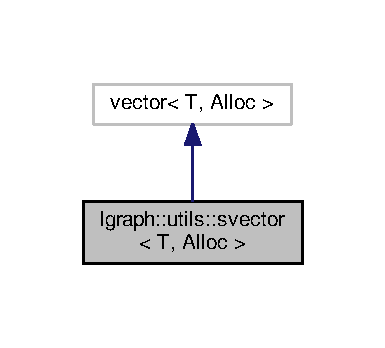
\includegraphics[width=185pt]{classlgraph_1_1utils_1_1svector__inherit__graph}
\end{center}
\end{figure}


Collaboration diagram for lgraph\+:\+:utils\+:\+:svector$<$ T, Alloc $>$\+:
\nopagebreak
\begin{figure}[H]
\begin{center}
\leavevmode
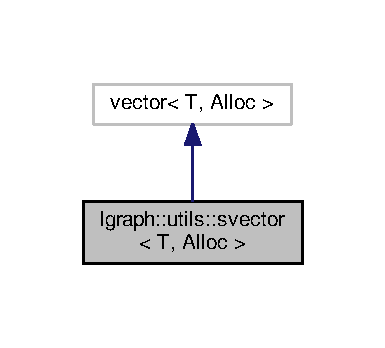
\includegraphics[width=185pt]{classlgraph_1_1utils_1_1svector__coll__graph}
\end{center}
\end{figure}
\subsection*{Public Member Functions}
\begin{DoxyCompactItemize}
\item 
\hyperlink{classlgraph_1_1utils_1_1svector_ae2587ed7933a70b8367e178dd61f90f9}{svector} ()\hypertarget{classlgraph_1_1utils_1_1svector_ae2587ed7933a70b8367e178dd61f90f9}{}\label{classlgraph_1_1utils_1_1svector_ae2587ed7933a70b8367e178dd61f90f9}

\begin{DoxyCompactList}\small\item\em Empty constructor. \end{DoxyCompactList}\item 
\hyperlink{classlgraph_1_1utils_1_1svector_aae71cfdb8e4d66c25a255b4a6bc7ad1c}{svector} (size\+\_\+t n)\hypertarget{classlgraph_1_1utils_1_1svector_aae71cfdb8e4d66c25a255b4a6bc7ad1c}{}\label{classlgraph_1_1utils_1_1svector_aae71cfdb8e4d66c25a255b4a6bc7ad1c}

\begin{DoxyCompactList}\small\item\em Construct a shortened vector that holds {\itshape n} elements. \end{DoxyCompactList}\item 
\hyperlink{classlgraph_1_1utils_1_1svector_a350de4ad59381c976905881480b0ed05}{svector} (size\+\_\+t n, const T \&v)\hypertarget{classlgraph_1_1utils_1_1svector_a350de4ad59381c976905881480b0ed05}{}\label{classlgraph_1_1utils_1_1svector_a350de4ad59381c976905881480b0ed05}

\begin{DoxyCompactList}\small\item\em Construct a shortened vector that holds {\itshape n} elements, all of them being {\itshape v}. \end{DoxyCompactList}\item 
\hyperlink{classlgraph_1_1utils_1_1svector_a32558a0ffa1a78f192d4294e37922cbe}{$\sim$svector} ()\hypertarget{classlgraph_1_1utils_1_1svector_a32558a0ffa1a78f192d4294e37922cbe}{}\label{classlgraph_1_1utils_1_1svector_a32558a0ffa1a78f192d4294e37922cbe}

\begin{DoxyCompactList}\small\item\em Destructor. \end{DoxyCompactList}\item 
void \hyperlink{classlgraph_1_1utils_1_1svector_a14ffd05a33eeae26ddb0909d8f64ad28}{add} (const T \&v)
\begin{DoxyCompactList}\small\item\em Adds an element to this vector. \end{DoxyCompactList}\item 
void \hyperlink{classlgraph_1_1utils_1_1svector_a9d377cbaa26f09a862334363e2d889cc}{remove} (size\+\_\+t i)
\begin{DoxyCompactList}\small\item\em Removes the element in the i-\/th position of this vector. \end{DoxyCompactList}\item 
void \hyperlink{classlgraph_1_1utils_1_1svector_ac2199e164429f7469decfa9d8f033069}{sort} ()
\begin{DoxyCompactList}\small\item\em Sorts the elements of this vector. \end{DoxyCompactList}\item 
size\+\_\+t \hyperlink{classlgraph_1_1utils_1_1svector_a36428d7450874d526ced6f1e8e0fe353}{n\+\_\+elems} () const 
\begin{DoxyCompactList}\small\item\em Returns the number of elements in this vector. \end{DoxyCompactList}\item 
bool \hyperlink{classlgraph_1_1utils_1_1svector_ab17c14abafd02d01a0e1f8230ed23680}{contains} (const T \&v) const 
\begin{DoxyCompactList}\small\item\em Looks for an element equal to {\itshape v} in the vector. \end{DoxyCompactList}\item 
bool \hyperlink{classlgraph_1_1utils_1_1svector_aed55a2e91d3ba407b5268ba339dddd81}{position} (const T \&v, size\+\_\+t \&pos) const 
\begin{DoxyCompactList}\small\item\em Looks for an element {\itshape v} in the vector and stores its position in {\itshape pos}. \end{DoxyCompactList}\end{DoxyCompactItemize}
\subsection*{Private Attributes}
\begin{DoxyCompactItemize}
\item 
size\+\_\+t \hyperlink{classlgraph_1_1utils_1_1svector_a7ef963c079c7dc8a6a559ceef81a241f}{idx}
\begin{DoxyCompactList}\small\item\em Pointer to the next position available in the vector. \end{DoxyCompactList}\end{DoxyCompactItemize}
\subsection*{Friends}
\begin{DoxyCompactItemize}
\item 
ostream \& \hyperlink{classlgraph_1_1utils_1_1svector_a57b29ed979371b1ad0a9ba9932f6531c}{operator$<$$<$} (ostream \&os, const \hyperlink{classlgraph_1_1utils_1_1svector}{svector} \&v)
\begin{DoxyCompactList}\small\item\em Outputs in an ostream object the contents of this vector. \end{DoxyCompactList}\end{DoxyCompactItemize}


\subsection{Detailed Description}
\subsubsection*{template$<$class T, class Alloc = allocator$<$\+T$>$$>$\\*
class lgraph\+::utils\+::svector$<$ T, Alloc $>$}

Shortened vector. 

This class implements a little shortcut in vectors for the ease of inserting/deleting elements without having to use iterators.

A pointer determines the position next to the last element of the vector. Any element added to the vector is placed where \hyperlink{classlgraph_1_1utils_1_1svector_a7ef963c079c7dc8a6a559ceef81a241f}{idx} points at and then \hyperlink{classlgraph_1_1utils_1_1svector_a7ef963c079c7dc8a6a559ceef81a241f}{idx} is incremented. Any element removed is moved at the position before \hyperlink{classlgraph_1_1utils_1_1svector_a7ef963c079c7dc8a6a559ceef81a241f}{idx} and then \hyperlink{classlgraph_1_1utils_1_1svector_a7ef963c079c7dc8a6a559ceef81a241f}{idx} is decremented.


\begin{DoxyParams}{Parameters}
{\em T} & The type of the elements stored. Must implement the \textquotesingle{}=\textquotesingle{} operator. \\
\hline
{\em Alloc} & The allocator for the elements of type {\itshape T}. See the documentation for C++\textquotesingle{}s vectors for more details (\href{http://en.cppreference.com/w/cpp/container/vector}{\tt http\+://en.\+cppreference.\+com/w/cpp/container/vector}) \\
\hline
\end{DoxyParams}


\subsection{Member Function Documentation}
\index{lgraph\+::utils\+::svector@{lgraph\+::utils\+::svector}!add@{add}}
\index{add@{add}!lgraph\+::utils\+::svector@{lgraph\+::utils\+::svector}}
\subsubsection[{\texorpdfstring{add(const T \&v)}{add(const T &v)}}]{\setlength{\rightskip}{0pt plus 5cm}template$<$class T , class Alloc $>$ void {\bf lgraph\+::utils\+::svector}$<$ T, Alloc $>$\+::add (
\begin{DoxyParamCaption}
\item[{const T \&}]{v}
\end{DoxyParamCaption}
)}\hypertarget{classlgraph_1_1utils_1_1svector_a14ffd05a33eeae26ddb0909d8f64ad28}{}\label{classlgraph_1_1utils_1_1svector_a14ffd05a33eeae26ddb0909d8f64ad28}


Adds an element to this vector. 

If \hyperlink{classlgraph_1_1utils_1_1svector_a7ef963c079c7dc8a6a559ceef81a241f}{idx} is equal to size() then the method push\+\_\+back() is called. Otherwise, element {\itshape v} is copied to the position pointed by \hyperlink{classlgraph_1_1utils_1_1svector_a7ef963c079c7dc8a6a559ceef81a241f}{idx} and then \hyperlink{classlgraph_1_1utils_1_1svector_a7ef963c079c7dc8a6a559ceef81a241f}{idx} is incremented. 
\begin{DoxyParams}{Parameters}
{\em v} & Value to be added \\
\hline
\end{DoxyParams}
\index{lgraph\+::utils\+::svector@{lgraph\+::utils\+::svector}!contains@{contains}}
\index{contains@{contains}!lgraph\+::utils\+::svector@{lgraph\+::utils\+::svector}}
\subsubsection[{\texorpdfstring{contains(const T \&v) const }{contains(const T &v) const }}]{\setlength{\rightskip}{0pt plus 5cm}template$<$class T , class Alloc $>$ bool {\bf lgraph\+::utils\+::svector}$<$ T, Alloc $>$\+::contains (
\begin{DoxyParamCaption}
\item[{const T \&}]{v}
\end{DoxyParamCaption}
) const}\hypertarget{classlgraph_1_1utils_1_1svector_ab17c14abafd02d01a0e1f8230ed23680}{}\label{classlgraph_1_1utils_1_1svector_ab17c14abafd02d01a0e1f8230ed23680}


Looks for an element equal to {\itshape v} in the vector. 

Performs a linear search on the contents of the vector. 
\begin{DoxyParams}{Parameters}
{\em v} & T\+He element to be searched \\
\hline
\end{DoxyParams}
\begin{DoxyReturn}{Returns}
Returns true if there is an element equal to {\itshape v} in the vector. 
\end{DoxyReturn}
\index{lgraph\+::utils\+::svector@{lgraph\+::utils\+::svector}!n\+\_\+elems@{n\+\_\+elems}}
\index{n\+\_\+elems@{n\+\_\+elems}!lgraph\+::utils\+::svector@{lgraph\+::utils\+::svector}}
\subsubsection[{\texorpdfstring{n\+\_\+elems() const }{n_elems() const }}]{\setlength{\rightskip}{0pt plus 5cm}template$<$class T , class Alloc $>$ size\+\_\+t {\bf lgraph\+::utils\+::svector}$<$ T, Alloc $>$\+::n\+\_\+elems (
\begin{DoxyParamCaption}
{}
\end{DoxyParamCaption}
) const}\hypertarget{classlgraph_1_1utils_1_1svector_a36428d7450874d526ced6f1e8e0fe353}{}\label{classlgraph_1_1utils_1_1svector_a36428d7450874d526ced6f1e8e0fe353}


Returns the number of elements in this vector. 

\begin{DoxyReturn}{Returns}
Returns the value of \hyperlink{classlgraph_1_1utils_1_1svector_a7ef963c079c7dc8a6a559ceef81a241f}{idx} 
\end{DoxyReturn}
\index{lgraph\+::utils\+::svector@{lgraph\+::utils\+::svector}!position@{position}}
\index{position@{position}!lgraph\+::utils\+::svector@{lgraph\+::utils\+::svector}}
\subsubsection[{\texorpdfstring{position(const T \&v, size\+\_\+t \&pos) const }{position(const T &v, size_t &pos) const }}]{\setlength{\rightskip}{0pt plus 5cm}template$<$class T , class Alloc $>$ bool {\bf lgraph\+::utils\+::svector}$<$ T, Alloc $>$\+::position (
\begin{DoxyParamCaption}
\item[{const T \&}]{v, }
\item[{size\+\_\+t \&}]{pos}
\end{DoxyParamCaption}
) const}\hypertarget{classlgraph_1_1utils_1_1svector_aed55a2e91d3ba407b5268ba339dddd81}{}\label{classlgraph_1_1utils_1_1svector_aed55a2e91d3ba407b5268ba339dddd81}


Looks for an element {\itshape v} in the vector and stores its position in {\itshape pos}. 


\begin{DoxyParams}[1]{Parameters}
\mbox{\tt in}  & {\em v} & The element to be searched \\
\hline
\mbox{\tt out}  & {\em pos} & The position of {\itshape v} in the vector. \\
\hline
\end{DoxyParams}
\begin{DoxyReturn}{Returns}
Returns true if {\itshape v} is in the vector. 
\end{DoxyReturn}
\index{lgraph\+::utils\+::svector@{lgraph\+::utils\+::svector}!remove@{remove}}
\index{remove@{remove}!lgraph\+::utils\+::svector@{lgraph\+::utils\+::svector}}
\subsubsection[{\texorpdfstring{remove(size\+\_\+t i)}{remove(size_t i)}}]{\setlength{\rightskip}{0pt plus 5cm}template$<$class T , class Alloc $>$ void {\bf lgraph\+::utils\+::svector}$<$ T, Alloc $>$\+::remove (
\begin{DoxyParamCaption}
\item[{size\+\_\+t}]{i}
\end{DoxyParamCaption}
)}\hypertarget{classlgraph_1_1utils_1_1svector_a9d377cbaa26f09a862334363e2d889cc}{}\label{classlgraph_1_1utils_1_1svector_a9d377cbaa26f09a862334363e2d889cc}


Removes the element in the i-\/th position of this vector. 

Places the element in the {\itshape i-\/th} position of this vector and then decrements the value of \hyperlink{classlgraph_1_1utils_1_1svector_a7ef963c079c7dc8a6a559ceef81a241f}{idx}. 
\begin{DoxyParams}{Parameters}
{\em i} & The index of the element to be removed. \\
\hline
\end{DoxyParams}
\index{lgraph\+::utils\+::svector@{lgraph\+::utils\+::svector}!sort@{sort}}
\index{sort@{sort}!lgraph\+::utils\+::svector@{lgraph\+::utils\+::svector}}
\subsubsection[{\texorpdfstring{sort()}{sort()}}]{\setlength{\rightskip}{0pt plus 5cm}template$<$class T , class Alloc $>$ void {\bf lgraph\+::utils\+::svector}$<$ T, Alloc $>$\+::sort (
\begin{DoxyParamCaption}
{}
\end{DoxyParamCaption}
)}\hypertarget{classlgraph_1_1utils_1_1svector_ac2199e164429f7469decfa9d8f033069}{}\label{classlgraph_1_1utils_1_1svector_ac2199e164429f7469decfa9d8f033069}


Sorts the elements of this vector. 

Sorts the elements in positions \mbox{[}0,..,\hyperlink{classlgraph_1_1utils_1_1svector_a7ef963c079c7dc8a6a559ceef81a241f}{idx}) 

\subsection{Friends And Related Function Documentation}
\index{lgraph\+::utils\+::svector@{lgraph\+::utils\+::svector}!operator$<$$<$@{operator$<$$<$}}
\index{operator$<$$<$@{operator$<$$<$}!lgraph\+::utils\+::svector@{lgraph\+::utils\+::svector}}
\subsubsection[{\texorpdfstring{operator$<$$<$}{operator<<}}]{\setlength{\rightskip}{0pt plus 5cm}template$<$class T , class Alloc  = allocator$<$\+T$>$$>$ ostream\& operator$<$$<$ (
\begin{DoxyParamCaption}
\item[{ostream \&}]{os, }
\item[{const {\bf svector}$<$ T, Alloc $>$ \&}]{v}
\end{DoxyParamCaption}
)\hspace{0.3cm}{\ttfamily [friend]}}\hypertarget{classlgraph_1_1utils_1_1svector_a57b29ed979371b1ad0a9ba9932f6531c}{}\label{classlgraph_1_1utils_1_1svector_a57b29ed979371b1ad0a9ba9932f6531c}


Outputs in an ostream object the contents of this vector. 

The contents passed to the ostream object are all those elements whose index is strictly below \hyperlink{classlgraph_1_1utils_1_1svector_a7ef963c079c7dc8a6a559ceef81a241f}{idx}. 

\subsection{Member Data Documentation}
\index{lgraph\+::utils\+::svector@{lgraph\+::utils\+::svector}!idx@{idx}}
\index{idx@{idx}!lgraph\+::utils\+::svector@{lgraph\+::utils\+::svector}}
\subsubsection[{\texorpdfstring{idx}{idx}}]{\setlength{\rightskip}{0pt plus 5cm}template$<$class T , class Alloc  = allocator$<$\+T$>$$>$ size\+\_\+t {\bf lgraph\+::utils\+::svector}$<$ T, Alloc $>$\+::idx\hspace{0.3cm}{\ttfamily [private]}}\hypertarget{classlgraph_1_1utils_1_1svector_a7ef963c079c7dc8a6a559ceef81a241f}{}\label{classlgraph_1_1utils_1_1svector_a7ef963c079c7dc8a6a559ceef81a241f}


Pointer to the next position available in the vector. 

For example\+: \textbackslash{}/ contents\+: 0 1 2 3 \+\_\+\+\_\+ \hyperlink{classlgraph_1_1utils_1_1svector_a7ef963c079c7dc8a6a559ceef81a241f}{idx} points at the position after element 3 any new element added will be stored in the position pointed by \hyperlink{classlgraph_1_1utils_1_1svector_a7ef963c079c7dc8a6a559ceef81a241f}{idx} 

The documentation for this class was generated from the following files\+:\begin{DoxyCompactItemize}
\item 
lgraph/data\+\_\+structures/svector.\+hpp\item 
lgraph/data\+\_\+structures/svector.\+cpp\end{DoxyCompactItemize}

\hypertarget{classlgraph_1_1utils_1_1uugraph}{}\section{lgraph\+:\+:utils\+:\+:uugraph Class Reference}
\label{classlgraph_1_1utils_1_1uugraph}\index{lgraph\+::utils\+::uugraph@{lgraph\+::utils\+::uugraph}}


Unweighted undirected (ux) graphs.  




{\ttfamily \#include $<$uugraph.\+hpp$>$}



Inheritance diagram for lgraph\+:\+:utils\+:\+:uugraph\+:\nopagebreak
\begin{figure}[H]
\begin{center}
\leavevmode
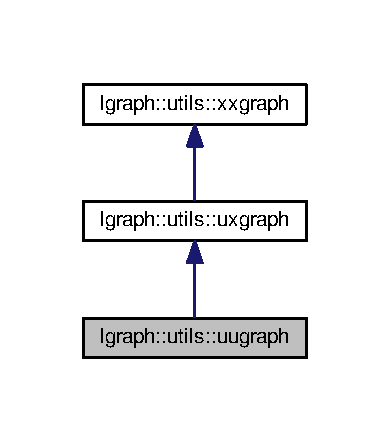
\includegraphics[width=187pt]{classlgraph_1_1utils_1_1uugraph__inherit__graph}
\end{center}
\end{figure}


Collaboration diagram for lgraph\+:\+:utils\+:\+:uugraph\+:\nopagebreak
\begin{figure}[H]
\begin{center}
\leavevmode
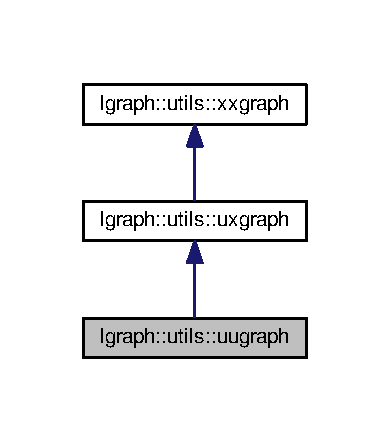
\includegraphics[width=187pt]{classlgraph_1_1utils_1_1uugraph__coll__graph}
\end{center}
\end{figure}
\subsection*{Public Member Functions}
\begin{DoxyCompactItemize}
\item 
\hyperlink{classlgraph_1_1utils_1_1uugraph_a8b92ac8dccde231b9d35fbe20be8d1ed}{uugraph} ()\hypertarget{classlgraph_1_1utils_1_1uugraph_a8b92ac8dccde231b9d35fbe20be8d1ed}{}\label{classlgraph_1_1utils_1_1uugraph_a8b92ac8dccde231b9d35fbe20be8d1ed}

\begin{DoxyCompactList}\small\item\em Constructor. \end{DoxyCompactList}\item 
\hyperlink{classlgraph_1_1utils_1_1uugraph_a7c990a2d79beea5f05bb9d4c13071cf6}{$\sim$uugraph} ()\hypertarget{classlgraph_1_1utils_1_1uugraph_a7c990a2d79beea5f05bb9d4c13071cf6}{}\label{classlgraph_1_1utils_1_1uugraph_a7c990a2d79beea5f05bb9d4c13071cf6}

\begin{DoxyCompactList}\small\item\em Destructor. \end{DoxyCompactList}\item 
void \hyperlink{classlgraph_1_1utils_1_1uugraph_ad1e6036f836c981ab8f4b540cbaa817e}{add\+\_\+edge} (const \hyperlink{namespacelgraph_1_1utils_a6510284ce1b1ae5dc97ce5d2de426e10}{edge} \&e)
\begin{DoxyCompactList}\small\item\em Adds an edge to this graph. \end{DoxyCompactList}\item 
void \hyperlink{classlgraph_1_1utils_1_1uugraph_a3729660ecdd5d7ed338f0cd687403cbf}{add\+\_\+edge} (\hyperlink{namespacelgraph_1_1utils_a7bd66ede3805ef121bc2835bd48de0cf}{node} u, \hyperlink{namespacelgraph_1_1utils_a7bd66ede3805ef121bc2835bd48de0cf}{node} v)
\begin{DoxyCompactList}\small\item\em Adds an edge between nodes {\itshape u} and {\itshape v}. \end{DoxyCompactList}\item 
void \hyperlink{classlgraph_1_1utils_1_1uugraph_a12591fd958878113b373040b4c164f14}{remove\+\_\+edge} (const \hyperlink{namespacelgraph_1_1utils_a6510284ce1b1ae5dc97ce5d2de426e10}{edge} \&e)
\begin{DoxyCompactList}\small\item\em Removes an edge from this graph. \end{DoxyCompactList}\item 
void \hyperlink{classlgraph_1_1utils_1_1uugraph_ae564207e9c3887aa6be115bce28c66b8}{remove\+\_\+edge} (\hyperlink{namespacelgraph_1_1utils_a7bd66ede3805ef121bc2835bd48de0cf}{node} u, \hyperlink{namespacelgraph_1_1utils_a7bd66ede3805ef121bc2835bd48de0cf}{node} v)
\begin{DoxyCompactList}\small\item\em Removes an edge from this graph. \end{DoxyCompactList}\item 
bool \hyperlink{classlgraph_1_1utils_1_1uugraph_a1970a2f371f20284478246a83292f9bb}{has\+\_\+edge} (\hyperlink{namespacelgraph_1_1utils_a7bd66ede3805ef121bc2835bd48de0cf}{node} u, \hyperlink{namespacelgraph_1_1utils_a7bd66ede3805ef121bc2835bd48de0cf}{node} v) const 
\begin{DoxyCompactList}\small\item\em Returns true if there is an edge between nodes {\itshape u} and {\itshape v}. \end{DoxyCompactList}\item 
bool \hyperlink{classlgraph_1_1utils_1_1uugraph_a20a86c5b56527e8abcbb90bae95d6605}{is\+\_\+directed} () const 
\begin{DoxyCompactList}\small\item\em Returns whether the graph is directed or undirected. \end{DoxyCompactList}\item 
void \hyperlink{classlgraph_1_1utils_1_1uxgraph_ab1e7ab39be6e8ca6149eef47dd51b155}{init} (size\+\_\+t n)
\begin{DoxyCompactList}\small\item\em Initialises the attributes of a graph with {\itshape n} nodes. \end{DoxyCompactList}\item 
void \hyperlink{classlgraph_1_1utils_1_1uxgraph_af6f7c0a2dc67706a07bd58f06b3dcf9f}{add\+\_\+edges} (const vector$<$ \hyperlink{namespacelgraph_1_1utils_a6510284ce1b1ae5dc97ce5d2de426e10}{edge} $>$ \&edge\+\_\+list)
\begin{DoxyCompactList}\small\item\em Adds all edges taken from a list. \end{DoxyCompactList}\item 
void \hyperlink{classlgraph_1_1utils_1_1uxgraph_a83e447e3c405700f36a1cce1c227f3f1}{remove\+\_\+edges} (const vector$<$ \hyperlink{namespacelgraph_1_1utils_a6510284ce1b1ae5dc97ce5d2de426e10}{edge} $>$ \&edge\+\_\+list)
\begin{DoxyCompactList}\small\item\em Removes all edges taken from a list. \end{DoxyCompactList}\item 
void \hyperlink{classlgraph_1_1utils_1_1uxgraph_ae76c83683dc7527fe5394d67437a7107}{clear} ()
\begin{DoxyCompactList}\small\item\em Deletes all memory used by the graph. \end{DoxyCompactList}\item 
bool \hyperlink{classlgraph_1_1utils_1_1uxgraph_ae1c3f40bb80ab20c2de96735ccde7b3f}{is\+\_\+weighted} () const \hypertarget{classlgraph_1_1utils_1_1uxgraph_ae1c3f40bb80ab20c2de96735ccde7b3f}{}\label{classlgraph_1_1utils_1_1uxgraph_ae1c3f40bb80ab20c2de96735ccde7b3f}

\begin{DoxyCompactList}\small\item\em Returns whether this graph is weighted or not (returns false). \end{DoxyCompactList}\item 
void \hyperlink{classlgraph_1_1utils_1_1uxgraph_ade877f3a9cf71d844cfe7b6c4f8aae10}{edges} (vector$<$ \hyperlink{namespacelgraph_1_1utils_a6510284ce1b1ae5dc97ce5d2de426e10}{edge} $>$ \&all\+\_\+edges) const 
\begin{DoxyCompactList}\small\item\em Returns all unique edges of this graph. \end{DoxyCompactList}\item 
bool \hyperlink{classlgraph_1_1utils_1_1uxgraph_a8328003e12383f0ff3f344aa6a239345}{read\+\_\+from\+\_\+file} (const string \&filename)\hypertarget{classlgraph_1_1utils_1_1uxgraph_a8328003e12383f0ff3f344aa6a239345}{}\label{classlgraph_1_1utils_1_1uxgraph_a8328003e12383f0ff3f344aa6a239345}

\begin{DoxyCompactList}\small\item\em Reads the graph from a file. \end{DoxyCompactList}\item 
bool \hyperlink{classlgraph_1_1utils_1_1uxgraph_a3e8b1f79b060234dced303a4171fae92}{read\+\_\+from\+\_\+file} (const char $\ast$filename)\hypertarget{classlgraph_1_1utils_1_1uxgraph_a3e8b1f79b060234dced303a4171fae92}{}\label{classlgraph_1_1utils_1_1uxgraph_a3e8b1f79b060234dced303a4171fae92}

\begin{DoxyCompactList}\small\item\em Reads the graph from a file. \end{DoxyCompactList}\item 
bool \hyperlink{classlgraph_1_1utils_1_1uxgraph_a2aef5492b3c18e0a6a9a2e75e2ff9e04}{store\+\_\+in\+\_\+file} (const string \&filename)\hypertarget{classlgraph_1_1utils_1_1uxgraph_a2aef5492b3c18e0a6a9a2e75e2ff9e04}{}\label{classlgraph_1_1utils_1_1uxgraph_a2aef5492b3c18e0a6a9a2e75e2ff9e04}

\begin{DoxyCompactList}\small\item\em Stores the graph in a file. \end{DoxyCompactList}\item 
bool \hyperlink{classlgraph_1_1utils_1_1uxgraph_a1f54ad58bf346fe85e3c94c118854fc7}{store\+\_\+in\+\_\+file} (const char $\ast$filename)\hypertarget{classlgraph_1_1utils_1_1uxgraph_a1f54ad58bf346fe85e3c94c118854fc7}{}\label{classlgraph_1_1utils_1_1uxgraph_a1f54ad58bf346fe85e3c94c118854fc7}

\begin{DoxyCompactList}\small\item\em Stores the graph in a file. \end{DoxyCompactList}\item 
size\+\_\+t \hyperlink{classlgraph_1_1utils_1_1xxgraph_af41baf2c098e872731ad646aeec1b382}{add\+\_\+node} ()
\begin{DoxyCompactList}\small\item\em Adds one node to the graph. \end{DoxyCompactList}\item 
size\+\_\+t \hyperlink{classlgraph_1_1utils_1_1xxgraph_af4f3782c1a55f73c6f34f2f2c26fb404}{add\+\_\+n\+\_\+nodes} (\hyperlink{namespacelgraph_1_1utils_a7bd66ede3805ef121bc2835bd48de0cf}{node} n)
\begin{DoxyCompactList}\small\item\em Adds {\itshape n} nodes to the graph. \end{DoxyCompactList}\item 
bool \hyperlink{classlgraph_1_1utils_1_1xxgraph_a026ab064c2be26790cc1f547be2157c9}{has\+\_\+node} (\hyperlink{namespacelgraph_1_1utils_a7bd66ede3805ef121bc2835bd48de0cf}{node} u) const \hypertarget{classlgraph_1_1utils_1_1xxgraph_a026ab064c2be26790cc1f547be2157c9}{}\label{classlgraph_1_1utils_1_1xxgraph_a026ab064c2be26790cc1f547be2157c9}

\begin{DoxyCompactList}\small\item\em Returns true if node {\itshape u} is in this graph. \end{DoxyCompactList}\item 
size\+\_\+t \hyperlink{classlgraph_1_1utils_1_1xxgraph_ad345f1fbf1dee34e1579b5aea9aef9b2}{n\+\_\+nodes} () const 
\begin{DoxyCompactList}\small\item\em Returns the number of nodes. \end{DoxyCompactList}\item 
size\+\_\+t \hyperlink{classlgraph_1_1utils_1_1xxgraph_af3f7c3835406c2cbf70479ae1c0253c9}{n\+\_\+edges} () const 
\begin{DoxyCompactList}\small\item\em Returns the number of edges. \end{DoxyCompactList}\item 
void \hyperlink{classlgraph_1_1utils_1_1xxgraph_a99f83387aa9f59b861e675251be5a3ad}{nodes} (vector$<$ \hyperlink{namespacelgraph_1_1utils_a7bd66ede3805ef121bc2835bd48de0cf}{node} $>$ \&all\+\_\+nodes) const \hypertarget{classlgraph_1_1utils_1_1xxgraph_a99f83387aa9f59b861e675251be5a3ad}{}\label{classlgraph_1_1utils_1_1xxgraph_a99f83387aa9f59b861e675251be5a3ad}

\begin{DoxyCompactList}\small\item\em Returns all nodes (as integers) \end{DoxyCompactList}\item 
const \hyperlink{namespacelgraph_1_1utils_a0f2ef47028a466d26841709e705390ac}{neighbourhood} \& \hyperlink{classlgraph_1_1utils_1_1xxgraph_a2c5332c4663c2d52828893f095a68202}{get\+\_\+neighbours} (\hyperlink{namespacelgraph_1_1utils_a7bd66ede3805ef121bc2835bd48de0cf}{node} u) const 
\begin{DoxyCompactList}\small\item\em Returns the neighbourhood of node u. \end{DoxyCompactList}\item 
size\+\_\+t \hyperlink{classlgraph_1_1utils_1_1xxgraph_af588aa4c68004a31aa143024cdb6dcc9}{degree} (\hyperlink{namespacelgraph_1_1utils_a7bd66ede3805ef121bc2835bd48de0cf}{node} u) const 
\begin{DoxyCompactList}\small\item\em Returns the number of neighbours of u. \end{DoxyCompactList}\item 
void \hyperlink{classlgraph_1_1utils_1_1xxgraph_a401454762f6b4b69f13ab0a10729c457}{get\+\_\+adjacency\+\_\+matrix} (vector$<$ vector$<$ bool $>$ $>$ \&adj\+\_\+mat) const \hypertarget{classlgraph_1_1utils_1_1xxgraph_a401454762f6b4b69f13ab0a10729c457}{}\label{classlgraph_1_1utils_1_1xxgraph_a401454762f6b4b69f13ab0a10729c457}

\begin{DoxyCompactList}\small\item\em Returns the adjacency matrix of this graph. \end{DoxyCompactList}\item 
void \hyperlink{classlgraph_1_1utils_1_1xxgraph_aff73f5ac4cd2732caa0c528eb1c1833c}{get\+\_\+degree\+\_\+sequence} (map$<$ size\+\_\+t, size\+\_\+t $>$ \&ds) const 
\begin{DoxyCompactList}\small\item\em Returns the degree sequence of the graph. \end{DoxyCompactList}\item 
size\+\_\+t \hyperlink{classlgraph_1_1utils_1_1xxgraph_ad4f25a8b29c6f26bc1567cb9c5a564ba}{n\+\_\+triangles} () const 
\begin{DoxyCompactList}\small\item\em Returns the number of triangles in this graph. \end{DoxyCompactList}\end{DoxyCompactItemize}
\subsection*{Protected Member Functions}
\begin{DoxyCompactItemize}
\item 
void \hyperlink{classlgraph_1_1utils_1_1uugraph_a97cb6f05007d118895c8f0f2323c243f}{get\+\_\+unique\+\_\+edges} (set$<$ \hyperlink{namespacelgraph_1_1utils_a6510284ce1b1ae5dc97ce5d2de426e10}{edge} $>$ \&\hyperlink{classlgraph_1_1utils_1_1uxgraph_ade877f3a9cf71d844cfe7b6c4f8aae10}{edges}) const 
\begin{DoxyCompactList}\small\item\em Computes the list of unique edges of this graph. \end{DoxyCompactList}\item 
size\+\_\+t \hyperlink{classlgraph_1_1utils_1_1xxgraph_aac7ef2134cad9529869f1334de7892d9}{get\+\_\+neighbour\+\_\+position} (const \hyperlink{namespacelgraph_1_1utils_a0f2ef47028a466d26841709e705390ac}{neighbourhood} \&n, \hyperlink{namespacelgraph_1_1utils_a7bd66ede3805ef121bc2835bd48de0cf}{node} u) const 
\begin{DoxyCompactList}\small\item\em Returns the position of node {\itshape u\textquotesingle{}s} position in the neighbourhood {\itshape n}. \end{DoxyCompactList}\item 
void \hyperlink{classlgraph_1_1utils_1_1xxgraph_a2201aaff5e9ffa29a9b3abfde705dd46}{initialise\+\_\+adjacency\+\_\+list} (size\+\_\+t n)\hypertarget{classlgraph_1_1utils_1_1xxgraph_a2201aaff5e9ffa29a9b3abfde705dd46}{}\label{classlgraph_1_1utils_1_1xxgraph_a2201aaff5e9ffa29a9b3abfde705dd46}

\begin{DoxyCompactList}\small\item\em Initialise the list of neighbourhoods with {\itshape n} instances. \end{DoxyCompactList}\item 
void \hyperlink{classlgraph_1_1utils_1_1xxgraph_a6523402d0ec66918b95de23d2bee38fc}{clear\+\_\+adjacency\+\_\+list} ()\hypertarget{classlgraph_1_1utils_1_1xxgraph_a6523402d0ec66918b95de23d2bee38fc}{}\label{classlgraph_1_1utils_1_1xxgraph_a6523402d0ec66918b95de23d2bee38fc}

\begin{DoxyCompactList}\small\item\em Clear the list of neighbourhoods. \end{DoxyCompactList}\item 
void \hyperlink{classlgraph_1_1utils_1_1xxgraph_abd983125be7f2f2b9c812326a4a39e6d}{initialise\+\_\+parent\+\_\+graph} (size\+\_\+t n)
\begin{DoxyCompactList}\small\item\em Initialises the adjacency list of this graph. \end{DoxyCompactList}\item 
void \hyperlink{classlgraph_1_1utils_1_1xxgraph_a8d213a8dfe716d344dd51d1bd37c0e2c}{clear\+\_\+parent\+\_\+graph} ()
\begin{DoxyCompactList}\small\item\em Clears the adjacency list of this graph. \end{DoxyCompactList}\end{DoxyCompactItemize}
\subsection*{Protected Attributes}
\begin{DoxyCompactItemize}
\item 
vector$<$ \hyperlink{namespacelgraph_1_1utils_a0f2ef47028a466d26841709e705390ac}{neighbourhood} $>$ \hyperlink{classlgraph_1_1utils_1_1xxgraph_a1d5fda0d5aa89340f997428b982f966f}{adjacency\+\_\+list}\hypertarget{classlgraph_1_1utils_1_1xxgraph_a1d5fda0d5aa89340f997428b982f966f}{}\label{classlgraph_1_1utils_1_1xxgraph_a1d5fda0d5aa89340f997428b982f966f}

\begin{DoxyCompactList}\small\item\em The neighbourhood of every node. \end{DoxyCompactList}\item 
size\+\_\+t \hyperlink{classlgraph_1_1utils_1_1xxgraph_a217ebb1cd8946fedfbf94a9b22f7da48}{num\+\_\+edges}\hypertarget{classlgraph_1_1utils_1_1xxgraph_a217ebb1cd8946fedfbf94a9b22f7da48}{}\label{classlgraph_1_1utils_1_1xxgraph_a217ebb1cd8946fedfbf94a9b22f7da48}

\begin{DoxyCompactList}\small\item\em The amount of edges in this graph. \end{DoxyCompactList}\end{DoxyCompactItemize}


\subsection{Detailed Description}
Unweighted undirected (ux) graphs. 

This class implements the unweighted undirected graph data structure based on adjacency lists. 

\subsection{Member Function Documentation}
\index{lgraph\+::utils\+::uugraph@{lgraph\+::utils\+::uugraph}!add\+\_\+edge@{add\+\_\+edge}}
\index{add\+\_\+edge@{add\+\_\+edge}!lgraph\+::utils\+::uugraph@{lgraph\+::utils\+::uugraph}}
\subsubsection[{\texorpdfstring{add\+\_\+edge(const edge \&e)}{add_edge(const edge &e)}}]{\setlength{\rightskip}{0pt plus 5cm}void lgraph\+::utils\+::uugraph\+::add\+\_\+edge (
\begin{DoxyParamCaption}
\item[{const {\bf edge} \&}]{e}
\end{DoxyParamCaption}
)\hspace{0.3cm}{\ttfamily [virtual]}}\hypertarget{classlgraph_1_1utils_1_1uugraph_ad1e6036f836c981ab8f4b540cbaa817e}{}\label{classlgraph_1_1utils_1_1uugraph_ad1e6036f836c981ab8f4b540cbaa817e}


Adds an edge to this graph. 

The attribute \hyperlink{classlgraph_1_1utils_1_1xxgraph_a217ebb1cd8946fedfbf94a9b22f7da48}{num\+\_\+edges} is incremented by one. 
\begin{DoxyParams}{Parameters}
{\em e} & A pair of nodes \\
\hline
\end{DoxyParams}


Implements \hyperlink{classlgraph_1_1utils_1_1uxgraph_a737ddae69312e76211b51104dd1eea2f}{lgraph\+::utils\+::uxgraph}.

\index{lgraph\+::utils\+::uugraph@{lgraph\+::utils\+::uugraph}!add\+\_\+edge@{add\+\_\+edge}}
\index{add\+\_\+edge@{add\+\_\+edge}!lgraph\+::utils\+::uugraph@{lgraph\+::utils\+::uugraph}}
\subsubsection[{\texorpdfstring{add\+\_\+edge(node u, node v)}{add_edge(node u, node v)}}]{\setlength{\rightskip}{0pt plus 5cm}void lgraph\+::utils\+::uugraph\+::add\+\_\+edge (
\begin{DoxyParamCaption}
\item[{{\bf node}}]{u, }
\item[{{\bf node}}]{v}
\end{DoxyParamCaption}
)\hspace{0.3cm}{\ttfamily [virtual]}}\hypertarget{classlgraph_1_1utils_1_1uugraph_a3729660ecdd5d7ed338f0cd687403cbf}{}\label{classlgraph_1_1utils_1_1uugraph_a3729660ecdd5d7ed338f0cd687403cbf}


Adds an edge between nodes {\itshape u} and {\itshape v}. 

The attribute \hyperlink{classlgraph_1_1utils_1_1xxgraph_a217ebb1cd8946fedfbf94a9b22f7da48}{num\+\_\+edges} is incremented by one.


\begin{DoxyParams}{Parameters}
{\em u} & The fist node of the edge \\
\hline
{\em v} & The second node of the edge \\
\hline
\end{DoxyParams}


Implements \hyperlink{classlgraph_1_1utils_1_1uxgraph_a97bdb6946478fa12a44d9780a4dc3ee6}{lgraph\+::utils\+::uxgraph}.

\index{lgraph\+::utils\+::uugraph@{lgraph\+::utils\+::uugraph}!add\+\_\+edges@{add\+\_\+edges}}
\index{add\+\_\+edges@{add\+\_\+edges}!lgraph\+::utils\+::uugraph@{lgraph\+::utils\+::uugraph}}
\subsubsection[{\texorpdfstring{add\+\_\+edges(const vector$<$ edge $>$ \&edge\+\_\+list)}{add_edges(const vector< edge > &edge_list)}}]{\setlength{\rightskip}{0pt plus 5cm}void lgraph\+::utils\+::uxgraph\+::add\+\_\+edges (
\begin{DoxyParamCaption}
\item[{const vector$<$ {\bf edge} $>$ \&}]{edge\+\_\+list}
\end{DoxyParamCaption}
)\hspace{0.3cm}{\ttfamily [inherited]}}\hypertarget{classlgraph_1_1utils_1_1uxgraph_af6f7c0a2dc67706a07bd58f06b3dcf9f}{}\label{classlgraph_1_1utils_1_1uxgraph_af6f7c0a2dc67706a07bd58f06b3dcf9f}


Adds all edges taken from a list. 

The attribute \hyperlink{classlgraph_1_1utils_1_1xxgraph_a217ebb1cd8946fedfbf94a9b22f7da48}{num\+\_\+edges} is incremented as many times as elements there are in {\itshape edge\+\_\+list}. 
\begin{DoxyParams}{Parameters}
{\em edge\+\_\+list} & A list of pairs of nodes \\
\hline
\end{DoxyParams}
\index{lgraph\+::utils\+::uugraph@{lgraph\+::utils\+::uugraph}!add\+\_\+n\+\_\+nodes@{add\+\_\+n\+\_\+nodes}}
\index{add\+\_\+n\+\_\+nodes@{add\+\_\+n\+\_\+nodes}!lgraph\+::utils\+::uugraph@{lgraph\+::utils\+::uugraph}}
\subsubsection[{\texorpdfstring{add\+\_\+n\+\_\+nodes(node n)}{add_n_nodes(node n)}}]{\setlength{\rightskip}{0pt plus 5cm}size\+\_\+t lgraph\+::utils\+::xxgraph\+::add\+\_\+n\+\_\+nodes (
\begin{DoxyParamCaption}
\item[{{\bf node}}]{n}
\end{DoxyParamCaption}
)\hspace{0.3cm}{\ttfamily [inherited]}}\hypertarget{classlgraph_1_1utils_1_1xxgraph_af4f3782c1a55f73c6f34f2f2c26fb404}{}\label{classlgraph_1_1utils_1_1xxgraph_af4f3782c1a55f73c6f34f2f2c26fb404}


Adds {\itshape n} nodes to the graph. 

The nodes are assigned consecutive, increasing values. \begin{DoxyReturn}{Returns}
Returns the index of the last node. 
\end{DoxyReturn}
\index{lgraph\+::utils\+::uugraph@{lgraph\+::utils\+::uugraph}!add\+\_\+node@{add\+\_\+node}}
\index{add\+\_\+node@{add\+\_\+node}!lgraph\+::utils\+::uugraph@{lgraph\+::utils\+::uugraph}}
\subsubsection[{\texorpdfstring{add\+\_\+node()}{add_node()}}]{\setlength{\rightskip}{0pt plus 5cm}size\+\_\+t lgraph\+::utils\+::xxgraph\+::add\+\_\+node (
\begin{DoxyParamCaption}
{}
\end{DoxyParamCaption}
)\hspace{0.3cm}{\ttfamily [inherited]}}\hypertarget{classlgraph_1_1utils_1_1xxgraph_af41baf2c098e872731ad646aeec1b382}{}\label{classlgraph_1_1utils_1_1xxgraph_af41baf2c098e872731ad646aeec1b382}


Adds one node to the graph. 

\begin{DoxyReturn}{Returns}
Returns the index of the new node 
\end{DoxyReturn}
\index{lgraph\+::utils\+::uugraph@{lgraph\+::utils\+::uugraph}!clear@{clear}}
\index{clear@{clear}!lgraph\+::utils\+::uugraph@{lgraph\+::utils\+::uugraph}}
\subsubsection[{\texorpdfstring{clear()}{clear()}}]{\setlength{\rightskip}{0pt plus 5cm}void lgraph\+::utils\+::uxgraph\+::clear (
\begin{DoxyParamCaption}
{}
\end{DoxyParamCaption}
)\hspace{0.3cm}{\ttfamily [inherited]}}\hypertarget{classlgraph_1_1utils_1_1uxgraph_ae76c83683dc7527fe5394d67437a7107}{}\label{classlgraph_1_1utils_1_1uxgraph_ae76c83683dc7527fe5394d67437a7107}


Deletes all memory used by the graph. 

The value \hyperlink{classlgraph_1_1utils_1_1xxgraph_a217ebb1cd8946fedfbf94a9b22f7da48}{num\+\_\+edges} is set to 0. \index{lgraph\+::utils\+::uugraph@{lgraph\+::utils\+::uugraph}!clear\+\_\+parent\+\_\+graph@{clear\+\_\+parent\+\_\+graph}}
\index{clear\+\_\+parent\+\_\+graph@{clear\+\_\+parent\+\_\+graph}!lgraph\+::utils\+::uugraph@{lgraph\+::utils\+::uugraph}}
\subsubsection[{\texorpdfstring{clear\+\_\+parent\+\_\+graph()}{clear_parent_graph()}}]{\setlength{\rightskip}{0pt plus 5cm}void lgraph\+::utils\+::xxgraph\+::clear\+\_\+parent\+\_\+graph (
\begin{DoxyParamCaption}
{}
\end{DoxyParamCaption}
)\hspace{0.3cm}{\ttfamily [protected]}, {\ttfamily [inherited]}}\hypertarget{classlgraph_1_1utils_1_1xxgraph_a8d213a8dfe716d344dd51d1bd37c0e2c}{}\label{classlgraph_1_1utils_1_1xxgraph_a8d213a8dfe716d344dd51d1bd37c0e2c}


Clears the adjacency list of this graph. 

The value \hyperlink{classlgraph_1_1utils_1_1xxgraph_a217ebb1cd8946fedfbf94a9b22f7da48}{num\+\_\+edges} is set to 0. \index{lgraph\+::utils\+::uugraph@{lgraph\+::utils\+::uugraph}!degree@{degree}}
\index{degree@{degree}!lgraph\+::utils\+::uugraph@{lgraph\+::utils\+::uugraph}}
\subsubsection[{\texorpdfstring{degree(node u) const }{degree(node u) const }}]{\setlength{\rightskip}{0pt plus 5cm}size\+\_\+t lgraph\+::utils\+::xxgraph\+::degree (
\begin{DoxyParamCaption}
\item[{{\bf node}}]{u}
\end{DoxyParamCaption}
) const\hspace{0.3cm}{\ttfamily [inherited]}}\hypertarget{classlgraph_1_1utils_1_1xxgraph_af588aa4c68004a31aa143024cdb6dcc9}{}\label{classlgraph_1_1utils_1_1xxgraph_af588aa4c68004a31aa143024cdb6dcc9}


Returns the number of neighbours of u. 


\begin{DoxyParams}{Parameters}
{\em u} & The node whose neighbourhood size we want \\
\hline
\end{DoxyParams}
\begin{DoxyReturn}{Returns}
Returns the size of the neighbourhood of {\itshape u}, that is, the size of the list in \hyperlink{classlgraph_1_1utils_1_1xxgraph_a1d5fda0d5aa89340f997428b982f966f}{adjacency\+\_\+list}\mbox{[}u\mbox{]} 
\end{DoxyReturn}
\begin{DoxyPrecond}{Precondition}
{\itshape u} must be a node from the graph 
\end{DoxyPrecond}
\index{lgraph\+::utils\+::uugraph@{lgraph\+::utils\+::uugraph}!edges@{edges}}
\index{edges@{edges}!lgraph\+::utils\+::uugraph@{lgraph\+::utils\+::uugraph}}
\subsubsection[{\texorpdfstring{edges(vector$<$ edge $>$ \&all\+\_\+edges) const }{edges(vector< edge > &all_edges) const }}]{\setlength{\rightskip}{0pt plus 5cm}void lgraph\+::utils\+::uxgraph\+::edges (
\begin{DoxyParamCaption}
\item[{vector$<$ {\bf edge} $>$ \&}]{all\+\_\+edges}
\end{DoxyParamCaption}
) const\hspace{0.3cm}{\ttfamily [inherited]}}\hypertarget{classlgraph_1_1utils_1_1uxgraph_ade877f3a9cf71d844cfe7b6c4f8aae10}{}\label{classlgraph_1_1utils_1_1uxgraph_ade877f3a9cf71d844cfe7b6c4f8aae10}


Returns all unique edges of this graph. 

See method \hyperlink{classlgraph_1_1utils_1_1uxgraph_a042795f5d307b07396da89d50734234a}{get\+\_\+unique\+\_\+edges(set$<$edge$>$\&)const} for details. \index{lgraph\+::utils\+::uugraph@{lgraph\+::utils\+::uugraph}!get\+\_\+degree\+\_\+sequence@{get\+\_\+degree\+\_\+sequence}}
\index{get\+\_\+degree\+\_\+sequence@{get\+\_\+degree\+\_\+sequence}!lgraph\+::utils\+::uugraph@{lgraph\+::utils\+::uugraph}}
\subsubsection[{\texorpdfstring{get\+\_\+degree\+\_\+sequence(map$<$ size\+\_\+t, size\+\_\+t $>$ \&ds) const }{get_degree_sequence(map< size_t, size_t > &ds) const }}]{\setlength{\rightskip}{0pt plus 5cm}void lgraph\+::utils\+::xxgraph\+::get\+\_\+degree\+\_\+sequence (
\begin{DoxyParamCaption}
\item[{map$<$ size\+\_\+t, size\+\_\+t $>$ \&}]{ds}
\end{DoxyParamCaption}
) const\hspace{0.3cm}{\ttfamily [inherited]}}\hypertarget{classlgraph_1_1utils_1_1xxgraph_aff73f5ac4cd2732caa0c528eb1c1833c}{}\label{classlgraph_1_1utils_1_1xxgraph_aff73f5ac4cd2732caa0c528eb1c1833c}


Returns the degree sequence of the graph. 


\begin{DoxyParams}[1]{Parameters}
\mbox{\tt out}  & {\em ds} & A list of pairs\+: for each degree the amount of nodes in this graph that have that degree. The degree of a node is detailed in \hyperlink{classlgraph_1_1utils_1_1xxgraph_af588aa4c68004a31aa143024cdb6dcc9}{degree} \\
\hline
\end{DoxyParams}
\index{lgraph\+::utils\+::uugraph@{lgraph\+::utils\+::uugraph}!get\+\_\+neighbour\+\_\+position@{get\+\_\+neighbour\+\_\+position}}
\index{get\+\_\+neighbour\+\_\+position@{get\+\_\+neighbour\+\_\+position}!lgraph\+::utils\+::uugraph@{lgraph\+::utils\+::uugraph}}
\subsubsection[{\texorpdfstring{get\+\_\+neighbour\+\_\+position(const neighbourhood \&n, node u) const }{get_neighbour_position(const neighbourhood &n, node u) const }}]{\setlength{\rightskip}{0pt plus 5cm}size\+\_\+t lgraph\+::utils\+::xxgraph\+::get\+\_\+neighbour\+\_\+position (
\begin{DoxyParamCaption}
\item[{const {\bf neighbourhood} \&}]{n, }
\item[{{\bf node}}]{u}
\end{DoxyParamCaption}
) const\hspace{0.3cm}{\ttfamily [protected]}, {\ttfamily [inherited]}}\hypertarget{classlgraph_1_1utils_1_1xxgraph_aac7ef2134cad9529869f1334de7892d9}{}\label{classlgraph_1_1utils_1_1xxgraph_aac7ef2134cad9529869f1334de7892d9}


Returns the position of node {\itshape u\textquotesingle{}s} position in the neighbourhood {\itshape n}. 

If the position is equal to the number of elements of the list {\itshape n} then {\itshape u} is in the list. Performs a linear search to find it. 
\begin{DoxyParams}{Parameters}
{\em n} & The neighbourhood of a node in the graph \\
\hline
{\em u} & The node to look for in the neighbourhood \\
\hline
\end{DoxyParams}
\begin{DoxyReturn}{Returns}
Returns a value equal to the number of elements in the list {\itshape n} if node {\itshape u} is not in it. Returns a value smaller than that if otherwise. 
\end{DoxyReturn}
\index{lgraph\+::utils\+::uugraph@{lgraph\+::utils\+::uugraph}!get\+\_\+neighbours@{get\+\_\+neighbours}}
\index{get\+\_\+neighbours@{get\+\_\+neighbours}!lgraph\+::utils\+::uugraph@{lgraph\+::utils\+::uugraph}}
\subsubsection[{\texorpdfstring{get\+\_\+neighbours(node u) const }{get_neighbours(node u) const }}]{\setlength{\rightskip}{0pt plus 5cm}const {\bf neighbourhood} \& lgraph\+::utils\+::xxgraph\+::get\+\_\+neighbours (
\begin{DoxyParamCaption}
\item[{{\bf node}}]{u}
\end{DoxyParamCaption}
) const\hspace{0.3cm}{\ttfamily [inherited]}}\hypertarget{classlgraph_1_1utils_1_1xxgraph_a2c5332c4663c2d52828893f095a68202}{}\label{classlgraph_1_1utils_1_1xxgraph_a2c5332c4663c2d52828893f095a68202}


Returns the neighbourhood of node u. 


\begin{DoxyParams}{Parameters}
{\em u} & The node whose neighbourhood we want \\
\hline
\end{DoxyParams}
\begin{DoxyPrecond}{Precondition}
{\itshape u} must be a node from the graph 
\end{DoxyPrecond}
\index{lgraph\+::utils\+::uugraph@{lgraph\+::utils\+::uugraph}!get\+\_\+unique\+\_\+edges@{get\+\_\+unique\+\_\+edges}}
\index{get\+\_\+unique\+\_\+edges@{get\+\_\+unique\+\_\+edges}!lgraph\+::utils\+::uugraph@{lgraph\+::utils\+::uugraph}}
\subsubsection[{\texorpdfstring{get\+\_\+unique\+\_\+edges(set$<$ edge $>$ \&edges) const }{get_unique_edges(set< edge > &edges) const }}]{\setlength{\rightskip}{0pt plus 5cm}void lgraph\+::utils\+::uugraph\+::get\+\_\+unique\+\_\+edges (
\begin{DoxyParamCaption}
\item[{set$<$ {\bf edge} $>$ \&}]{edges}
\end{DoxyParamCaption}
) const\hspace{0.3cm}{\ttfamily [protected]}, {\ttfamily [virtual]}}\hypertarget{classlgraph_1_1utils_1_1uugraph_a97cb6f05007d118895c8f0f2323c243f}{}\label{classlgraph_1_1utils_1_1uugraph_a97cb6f05007d118895c8f0f2323c243f}


Computes the list of unique edges of this graph. 

Since this graph is undirected, the edge (u,v) is the same as (v,u). This method computes the list of edges so that the result is lexicographically sorted. An unweighted edge is a pair of indices each of which is within the interval \mbox{[}0,{\itshape n}) where {\itshape n} is the number of nodes of this graph.


\begin{DoxyParams}[1]{Parameters}
\mbox{\tt out}  & {\em edges} & The collection of edges \\
\hline
\end{DoxyParams}
\begin{DoxyReturn}{Returns}
Stores in \hyperlink{classlgraph_1_1utils_1_1uxgraph_ade877f3a9cf71d844cfe7b6c4f8aae10}{edges} the lexicographically sorted list of unweighted edges of this graph 
\end{DoxyReturn}


Implements \hyperlink{classlgraph_1_1utils_1_1uxgraph_a042795f5d307b07396da89d50734234a}{lgraph\+::utils\+::uxgraph}.

\index{lgraph\+::utils\+::uugraph@{lgraph\+::utils\+::uugraph}!has\+\_\+edge@{has\+\_\+edge}}
\index{has\+\_\+edge@{has\+\_\+edge}!lgraph\+::utils\+::uugraph@{lgraph\+::utils\+::uugraph}}
\subsubsection[{\texorpdfstring{has\+\_\+edge(node u, node v) const }{has_edge(node u, node v) const }}]{\setlength{\rightskip}{0pt plus 5cm}bool lgraph\+::utils\+::uugraph\+::has\+\_\+edge (
\begin{DoxyParamCaption}
\item[{{\bf node}}]{u, }
\item[{{\bf node}}]{v}
\end{DoxyParamCaption}
) const\hspace{0.3cm}{\ttfamily [virtual]}}\hypertarget{classlgraph_1_1utils_1_1uugraph_a1970a2f371f20284478246a83292f9bb}{}\label{classlgraph_1_1utils_1_1uugraph_a1970a2f371f20284478246a83292f9bb}


Returns true if there is an edge between nodes {\itshape u} and {\itshape v}. 

\begin{DoxyPrecond}{Precondition}
{\itshape u} and {\itshape v} must be in the graph 
\end{DoxyPrecond}


Implements \hyperlink{classlgraph_1_1utils_1_1xxgraph_a9e94100afc70b09049432f196550407c}{lgraph\+::utils\+::xxgraph}.

\index{lgraph\+::utils\+::uugraph@{lgraph\+::utils\+::uugraph}!init@{init}}
\index{init@{init}!lgraph\+::utils\+::uugraph@{lgraph\+::utils\+::uugraph}}
\subsubsection[{\texorpdfstring{init(size\+\_\+t n)}{init(size_t n)}}]{\setlength{\rightskip}{0pt plus 5cm}void lgraph\+::utils\+::uxgraph\+::init (
\begin{DoxyParamCaption}
\item[{size\+\_\+t}]{n}
\end{DoxyParamCaption}
)\hspace{0.3cm}{\ttfamily [virtual]}, {\ttfamily [inherited]}}\hypertarget{classlgraph_1_1utils_1_1uxgraph_ab1e7ab39be6e8ca6149eef47dd51b155}{}\label{classlgraph_1_1utils_1_1uxgraph_ab1e7ab39be6e8ca6149eef47dd51b155}


Initialises the attributes of a graph with {\itshape n} nodes. 

First, it clears all the memory allocated so far. Then, initialises all the attributes so that it can store all the necessary information. 
\begin{DoxyParams}{Parameters}
{\em n} & Number of nodes of the graph \\
\hline
\end{DoxyParams}


Implements \hyperlink{classlgraph_1_1utils_1_1xxgraph_a2ac8b3e71fa0550248c692a19ea04d0d}{lgraph\+::utils\+::xxgraph}.

\index{lgraph\+::utils\+::uugraph@{lgraph\+::utils\+::uugraph}!initialise\+\_\+parent\+\_\+graph@{initialise\+\_\+parent\+\_\+graph}}
\index{initialise\+\_\+parent\+\_\+graph@{initialise\+\_\+parent\+\_\+graph}!lgraph\+::utils\+::uugraph@{lgraph\+::utils\+::uugraph}}
\subsubsection[{\texorpdfstring{initialise\+\_\+parent\+\_\+graph(size\+\_\+t n)}{initialise_parent_graph(size_t n)}}]{\setlength{\rightskip}{0pt plus 5cm}void lgraph\+::utils\+::xxgraph\+::initialise\+\_\+parent\+\_\+graph (
\begin{DoxyParamCaption}
\item[{size\+\_\+t}]{n}
\end{DoxyParamCaption}
)\hspace{0.3cm}{\ttfamily [protected]}, {\ttfamily [inherited]}}\hypertarget{classlgraph_1_1utils_1_1xxgraph_abd983125be7f2f2b9c812326a4a39e6d}{}\label{classlgraph_1_1utils_1_1xxgraph_abd983125be7f2f2b9c812326a4a39e6d}


Initialises the adjacency list of this graph. 

The value \hyperlink{classlgraph_1_1utils_1_1xxgraph_a217ebb1cd8946fedfbf94a9b22f7da48}{num\+\_\+edges} is set to 0. \index{lgraph\+::utils\+::uugraph@{lgraph\+::utils\+::uugraph}!is\+\_\+directed@{is\+\_\+directed}}
\index{is\+\_\+directed@{is\+\_\+directed}!lgraph\+::utils\+::uugraph@{lgraph\+::utils\+::uugraph}}
\subsubsection[{\texorpdfstring{is\+\_\+directed() const }{is_directed() const }}]{\setlength{\rightskip}{0pt plus 5cm}bool lgraph\+::utils\+::uugraph\+::is\+\_\+directed (
\begin{DoxyParamCaption}
{}
\end{DoxyParamCaption}
) const\hspace{0.3cm}{\ttfamily [virtual]}}\hypertarget{classlgraph_1_1utils_1_1uugraph_a20a86c5b56527e8abcbb90bae95d6605}{}\label{classlgraph_1_1utils_1_1uugraph_a20a86c5b56527e8abcbb90bae95d6605}


Returns whether the graph is directed or undirected. 

\begin{DoxyReturn}{Returns}
Returns true if the graph is directed. Returns false if otherwise. 
\end{DoxyReturn}


Implements \hyperlink{classlgraph_1_1utils_1_1xxgraph_a154376b6e55c4654622eb17ce738b5bb}{lgraph\+::utils\+::xxgraph}.

\index{lgraph\+::utils\+::uugraph@{lgraph\+::utils\+::uugraph}!n\+\_\+edges@{n\+\_\+edges}}
\index{n\+\_\+edges@{n\+\_\+edges}!lgraph\+::utils\+::uugraph@{lgraph\+::utils\+::uugraph}}
\subsubsection[{\texorpdfstring{n\+\_\+edges() const }{n_edges() const }}]{\setlength{\rightskip}{0pt plus 5cm}size\+\_\+t lgraph\+::utils\+::xxgraph\+::n\+\_\+edges (
\begin{DoxyParamCaption}
{}
\end{DoxyParamCaption}
) const\hspace{0.3cm}{\ttfamily [inherited]}}\hypertarget{classlgraph_1_1utils_1_1xxgraph_af3f7c3835406c2cbf70479ae1c0253c9}{}\label{classlgraph_1_1utils_1_1xxgraph_af3f7c3835406c2cbf70479ae1c0253c9}


Returns the number of edges. 

\begin{DoxyReturn}{Returns}
Returns the value \hyperlink{classlgraph_1_1utils_1_1xxgraph_a217ebb1cd8946fedfbf94a9b22f7da48}{num\+\_\+edges} 
\end{DoxyReturn}
\index{lgraph\+::utils\+::uugraph@{lgraph\+::utils\+::uugraph}!n\+\_\+nodes@{n\+\_\+nodes}}
\index{n\+\_\+nodes@{n\+\_\+nodes}!lgraph\+::utils\+::uugraph@{lgraph\+::utils\+::uugraph}}
\subsubsection[{\texorpdfstring{n\+\_\+nodes() const }{n_nodes() const }}]{\setlength{\rightskip}{0pt plus 5cm}size\+\_\+t lgraph\+::utils\+::xxgraph\+::n\+\_\+nodes (
\begin{DoxyParamCaption}
{}
\end{DoxyParamCaption}
) const\hspace{0.3cm}{\ttfamily [inherited]}}\hypertarget{classlgraph_1_1utils_1_1xxgraph_ad345f1fbf1dee34e1579b5aea9aef9b2}{}\label{classlgraph_1_1utils_1_1xxgraph_ad345f1fbf1dee34e1579b5aea9aef9b2}


Returns the number of nodes. 

\begin{DoxyReturn}{Returns}
Returns the size of \hyperlink{classlgraph_1_1utils_1_1xxgraph_a1d5fda0d5aa89340f997428b982f966f}{adjacency\+\_\+list} 
\end{DoxyReturn}
\index{lgraph\+::utils\+::uugraph@{lgraph\+::utils\+::uugraph}!n\+\_\+triangles@{n\+\_\+triangles}}
\index{n\+\_\+triangles@{n\+\_\+triangles}!lgraph\+::utils\+::uugraph@{lgraph\+::utils\+::uugraph}}
\subsubsection[{\texorpdfstring{n\+\_\+triangles() const }{n_triangles() const }}]{\setlength{\rightskip}{0pt plus 5cm}size\+\_\+t lgraph\+::utils\+::xxgraph\+::n\+\_\+triangles (
\begin{DoxyParamCaption}
{}
\end{DoxyParamCaption}
) const\hspace{0.3cm}{\ttfamily [inherited]}}\hypertarget{classlgraph_1_1utils_1_1xxgraph_ad4f25a8b29c6f26bc1567cb9c5a564ba}{}\label{classlgraph_1_1utils_1_1xxgraph_ad4f25a8b29c6f26bc1567cb9c5a564ba}


Returns the number of triangles in this graph. 

\begin{DoxyReturn}{Returns}
Returns the number of cycles of length 3 
\end{DoxyReturn}
\index{lgraph\+::utils\+::uugraph@{lgraph\+::utils\+::uugraph}!remove\+\_\+edge@{remove\+\_\+edge}}
\index{remove\+\_\+edge@{remove\+\_\+edge}!lgraph\+::utils\+::uugraph@{lgraph\+::utils\+::uugraph}}
\subsubsection[{\texorpdfstring{remove\+\_\+edge(const edge \&e)}{remove_edge(const edge &e)}}]{\setlength{\rightskip}{0pt plus 5cm}void lgraph\+::utils\+::uugraph\+::remove\+\_\+edge (
\begin{DoxyParamCaption}
\item[{const {\bf edge} \&}]{e}
\end{DoxyParamCaption}
)\hspace{0.3cm}{\ttfamily [virtual]}}\hypertarget{classlgraph_1_1utils_1_1uugraph_a12591fd958878113b373040b4c164f14}{}\label{classlgraph_1_1utils_1_1uugraph_a12591fd958878113b373040b4c164f14}


Removes an edge from this graph. 

The attribute \hyperlink{classlgraph_1_1utils_1_1xxgraph_a217ebb1cd8946fedfbf94a9b22f7da48}{num\+\_\+edges} is decremented by one. 
\begin{DoxyParams}{Parameters}
{\em e} & A pair of nodes \\
\hline
\end{DoxyParams}


Implements \hyperlink{classlgraph_1_1utils_1_1uxgraph_a4773c30a317dd2cdc7fc3f2edaca4e9e}{lgraph\+::utils\+::uxgraph}.

\index{lgraph\+::utils\+::uugraph@{lgraph\+::utils\+::uugraph}!remove\+\_\+edge@{remove\+\_\+edge}}
\index{remove\+\_\+edge@{remove\+\_\+edge}!lgraph\+::utils\+::uugraph@{lgraph\+::utils\+::uugraph}}
\subsubsection[{\texorpdfstring{remove\+\_\+edge(node u, node v)}{remove_edge(node u, node v)}}]{\setlength{\rightskip}{0pt plus 5cm}void lgraph\+::utils\+::uugraph\+::remove\+\_\+edge (
\begin{DoxyParamCaption}
\item[{{\bf node}}]{u, }
\item[{{\bf node}}]{v}
\end{DoxyParamCaption}
)\hspace{0.3cm}{\ttfamily [virtual]}}\hypertarget{classlgraph_1_1utils_1_1uugraph_ae564207e9c3887aa6be115bce28c66b8}{}\label{classlgraph_1_1utils_1_1uugraph_ae564207e9c3887aa6be115bce28c66b8}


Removes an edge from this graph. 

The attribute \hyperlink{classlgraph_1_1utils_1_1xxgraph_a217ebb1cd8946fedfbf94a9b22f7da48}{num\+\_\+edges} is decremented by one. 
\begin{DoxyParams}{Parameters}
{\em u} & The fist node of the edge \\
\hline
{\em v} & The second node of the edge \\
\hline
\end{DoxyParams}


Implements \hyperlink{classlgraph_1_1utils_1_1uxgraph_a0f6d277efcb347ef085ddcdf5ae2da84}{lgraph\+::utils\+::uxgraph}.

\index{lgraph\+::utils\+::uugraph@{lgraph\+::utils\+::uugraph}!remove\+\_\+edges@{remove\+\_\+edges}}
\index{remove\+\_\+edges@{remove\+\_\+edges}!lgraph\+::utils\+::uugraph@{lgraph\+::utils\+::uugraph}}
\subsubsection[{\texorpdfstring{remove\+\_\+edges(const vector$<$ edge $>$ \&edge\+\_\+list)}{remove_edges(const vector< edge > &edge_list)}}]{\setlength{\rightskip}{0pt plus 5cm}void lgraph\+::utils\+::uxgraph\+::remove\+\_\+edges (
\begin{DoxyParamCaption}
\item[{const vector$<$ {\bf edge} $>$ \&}]{edge\+\_\+list}
\end{DoxyParamCaption}
)\hspace{0.3cm}{\ttfamily [inherited]}}\hypertarget{classlgraph_1_1utils_1_1uxgraph_a83e447e3c405700f36a1cce1c227f3f1}{}\label{classlgraph_1_1utils_1_1uxgraph_a83e447e3c405700f36a1cce1c227f3f1}


Removes all edges taken from a list. 

The attribute \hyperlink{classlgraph_1_1utils_1_1xxgraph_a217ebb1cd8946fedfbf94a9b22f7da48}{num\+\_\+edges} is decremented by one. 
\begin{DoxyParams}{Parameters}
{\em edge\+\_\+list} & A list of edges \\
\hline
\end{DoxyParams}


The documentation for this class was generated from the following files\+:\begin{DoxyCompactItemize}
\item 
lgraph/data\+\_\+structures/uugraph.\+hpp\item 
lgraph/data\+\_\+structures/uugraph.\+cpp\end{DoxyCompactItemize}

\hypertarget{classlgraph_1_1utils_1_1uxgraph}{}\section{lgraph\+:\+:utils\+:\+:uxgraph Class Reference}
\label{classlgraph_1_1utils_1_1uxgraph}\index{lgraph\+::utils\+::uxgraph@{lgraph\+::utils\+::uxgraph}}


Abstract class for unweighted (ux) graphs.  




{\ttfamily \#include $<$uxgraph.\+hpp$>$}



Inheritance diagram for lgraph\+:\+:utils\+:\+:uxgraph\+:\nopagebreak
\begin{figure}[H]
\begin{center}
\leavevmode
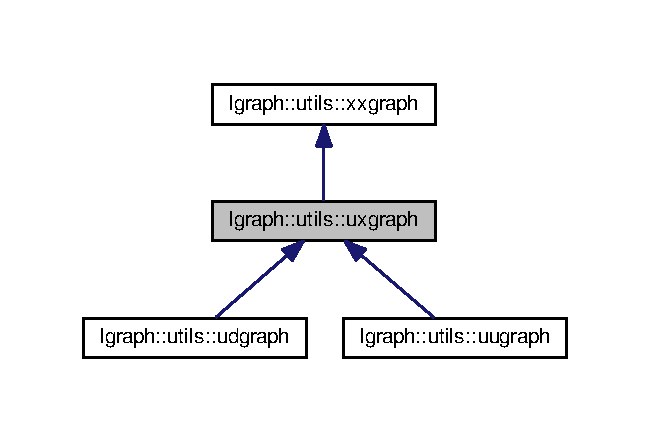
\includegraphics[width=312pt]{classlgraph_1_1utils_1_1uxgraph__inherit__graph}
\end{center}
\end{figure}


Collaboration diagram for lgraph\+:\+:utils\+:\+:uxgraph\+:\nopagebreak
\begin{figure}[H]
\begin{center}
\leavevmode
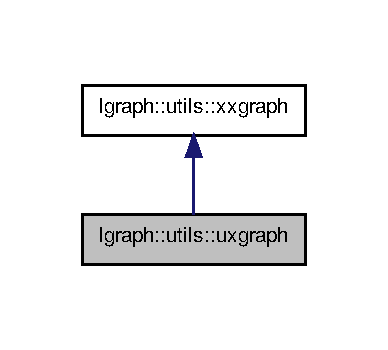
\includegraphics[width=187pt]{classlgraph_1_1utils_1_1uxgraph__coll__graph}
\end{center}
\end{figure}
\subsection*{Public Member Functions}
\begin{DoxyCompactItemize}
\item 
\hyperlink{classlgraph_1_1utils_1_1uxgraph_a20d8499ed3e0297b43b6dfc0c0042c44}{uxgraph} ()\hypertarget{classlgraph_1_1utils_1_1uxgraph_a20d8499ed3e0297b43b6dfc0c0042c44}{}\label{classlgraph_1_1utils_1_1uxgraph_a20d8499ed3e0297b43b6dfc0c0042c44}

\begin{DoxyCompactList}\small\item\em Constructor. \end{DoxyCompactList}\item 
virtual \hyperlink{classlgraph_1_1utils_1_1uxgraph_a1909df52804b8b883f43ccbf9c3226cf}{$\sim$uxgraph} ()\hypertarget{classlgraph_1_1utils_1_1uxgraph_a1909df52804b8b883f43ccbf9c3226cf}{}\label{classlgraph_1_1utils_1_1uxgraph_a1909df52804b8b883f43ccbf9c3226cf}

\begin{DoxyCompactList}\small\item\em Destructor. \end{DoxyCompactList}\item 
void \hyperlink{classlgraph_1_1utils_1_1uxgraph_ab1e7ab39be6e8ca6149eef47dd51b155}{init} (size\+\_\+t n)
\begin{DoxyCompactList}\small\item\em Initialises the attributes of a graph with {\itshape n} nodes. \end{DoxyCompactList}\item 
\hyperlink{classlgraph_1_1utils_1_1uxgraph}{uxgraph} \& \hyperlink{classlgraph_1_1utils_1_1uxgraph_aae32def9779a7af6261fe8637094c664}{operator=} (const \hyperlink{classlgraph_1_1utils_1_1uxgraph}{uxgraph} \&g)
\begin{DoxyCompactList}\small\item\em Assignation operator for undirected weighted graphs. \end{DoxyCompactList}\item 
virtual void \hyperlink{classlgraph_1_1utils_1_1uxgraph_a737ddae69312e76211b51104dd1eea2f}{add\+\_\+edge} (const \hyperlink{namespacelgraph_1_1utils_a6510284ce1b1ae5dc97ce5d2de426e10}{edge} \&e)=0
\begin{DoxyCompactList}\small\item\em Adds an edge to this graph. \end{DoxyCompactList}\item 
void \hyperlink{classlgraph_1_1utils_1_1uxgraph_af6f7c0a2dc67706a07bd58f06b3dcf9f}{add\+\_\+edges} (const vector$<$ \hyperlink{namespacelgraph_1_1utils_a6510284ce1b1ae5dc97ce5d2de426e10}{edge} $>$ \&edge\+\_\+list)
\begin{DoxyCompactList}\small\item\em Adds all edges taken from a list. \end{DoxyCompactList}\item 
virtual void \hyperlink{classlgraph_1_1utils_1_1uxgraph_a97bdb6946478fa12a44d9780a4dc3ee6}{add\+\_\+edge} (\hyperlink{namespacelgraph_1_1utils_a7bd66ede3805ef121bc2835bd48de0cf}{node} u, \hyperlink{namespacelgraph_1_1utils_a7bd66ede3805ef121bc2835bd48de0cf}{node} v)=0
\begin{DoxyCompactList}\small\item\em Adds an edge between nodes {\itshape u} and {\itshape v}. \end{DoxyCompactList}\item 
virtual void \hyperlink{classlgraph_1_1utils_1_1uxgraph_a4773c30a317dd2cdc7fc3f2edaca4e9e}{remove\+\_\+edge} (const \hyperlink{namespacelgraph_1_1utils_a6510284ce1b1ae5dc97ce5d2de426e10}{edge} \&e)=0
\begin{DoxyCompactList}\small\item\em Removes an edge from this graph. \end{DoxyCompactList}\item 
void \hyperlink{classlgraph_1_1utils_1_1uxgraph_a83e447e3c405700f36a1cce1c227f3f1}{remove\+\_\+edges} (const vector$<$ \hyperlink{namespacelgraph_1_1utils_a6510284ce1b1ae5dc97ce5d2de426e10}{edge} $>$ \&edge\+\_\+list)
\begin{DoxyCompactList}\small\item\em Removes all edges taken from a list. \end{DoxyCompactList}\item 
virtual void \hyperlink{classlgraph_1_1utils_1_1uxgraph_a0f6d277efcb347ef085ddcdf5ae2da84}{remove\+\_\+edge} (\hyperlink{namespacelgraph_1_1utils_a7bd66ede3805ef121bc2835bd48de0cf}{node} u, \hyperlink{namespacelgraph_1_1utils_a7bd66ede3805ef121bc2835bd48de0cf}{node} v)=0
\begin{DoxyCompactList}\small\item\em Removes an edge from this graph. \end{DoxyCompactList}\item 
void \hyperlink{classlgraph_1_1utils_1_1uxgraph_ae76c83683dc7527fe5394d67437a7107}{clear} ()
\begin{DoxyCompactList}\small\item\em Deletes all memory used by the graph. \end{DoxyCompactList}\item 
bool \hyperlink{classlgraph_1_1utils_1_1uxgraph_ae1c3f40bb80ab20c2de96735ccde7b3f}{is\+\_\+weighted} () const \hypertarget{classlgraph_1_1utils_1_1uxgraph_ae1c3f40bb80ab20c2de96735ccde7b3f}{}\label{classlgraph_1_1utils_1_1uxgraph_ae1c3f40bb80ab20c2de96735ccde7b3f}

\begin{DoxyCompactList}\small\item\em Returns whether this graph is weighted or not (returns false). \end{DoxyCompactList}\item 
void \hyperlink{classlgraph_1_1utils_1_1uxgraph_ade877f3a9cf71d844cfe7b6c4f8aae10}{edges} (vector$<$ \hyperlink{namespacelgraph_1_1utils_a6510284ce1b1ae5dc97ce5d2de426e10}{edge} $>$ \&all\+\_\+edges) const 
\begin{DoxyCompactList}\small\item\em Returns all unique edges of this graph. \end{DoxyCompactList}\item 
bool \hyperlink{classlgraph_1_1utils_1_1uxgraph_a8328003e12383f0ff3f344aa6a239345}{read\+\_\+from\+\_\+file} (const string \&filename)\hypertarget{classlgraph_1_1utils_1_1uxgraph_a8328003e12383f0ff3f344aa6a239345}{}\label{classlgraph_1_1utils_1_1uxgraph_a8328003e12383f0ff3f344aa6a239345}

\begin{DoxyCompactList}\small\item\em Reads the graph from a file. \end{DoxyCompactList}\item 
bool \hyperlink{classlgraph_1_1utils_1_1uxgraph_a3e8b1f79b060234dced303a4171fae92}{read\+\_\+from\+\_\+file} (const char $\ast$filename)\hypertarget{classlgraph_1_1utils_1_1uxgraph_a3e8b1f79b060234dced303a4171fae92}{}\label{classlgraph_1_1utils_1_1uxgraph_a3e8b1f79b060234dced303a4171fae92}

\begin{DoxyCompactList}\small\item\em Reads the graph from a file. \end{DoxyCompactList}\item 
bool \hyperlink{classlgraph_1_1utils_1_1uxgraph_a2aef5492b3c18e0a6a9a2e75e2ff9e04}{store\+\_\+in\+\_\+file} (const string \&filename)\hypertarget{classlgraph_1_1utils_1_1uxgraph_a2aef5492b3c18e0a6a9a2e75e2ff9e04}{}\label{classlgraph_1_1utils_1_1uxgraph_a2aef5492b3c18e0a6a9a2e75e2ff9e04}

\begin{DoxyCompactList}\small\item\em Stores the graph in a file. \end{DoxyCompactList}\item 
bool \hyperlink{classlgraph_1_1utils_1_1uxgraph_a1f54ad58bf346fe85e3c94c118854fc7}{store\+\_\+in\+\_\+file} (const char $\ast$filename)\hypertarget{classlgraph_1_1utils_1_1uxgraph_a1f54ad58bf346fe85e3c94c118854fc7}{}\label{classlgraph_1_1utils_1_1uxgraph_a1f54ad58bf346fe85e3c94c118854fc7}

\begin{DoxyCompactList}\small\item\em Stores the graph in a file. \end{DoxyCompactList}\item 
size\+\_\+t \hyperlink{classlgraph_1_1utils_1_1xxgraph_af41baf2c098e872731ad646aeec1b382}{add\+\_\+node} ()
\begin{DoxyCompactList}\small\item\em Adds one node to the graph. \end{DoxyCompactList}\item 
size\+\_\+t \hyperlink{classlgraph_1_1utils_1_1xxgraph_af4f3782c1a55f73c6f34f2f2c26fb404}{add\+\_\+n\+\_\+nodes} (\hyperlink{namespacelgraph_1_1utils_a7bd66ede3805ef121bc2835bd48de0cf}{node} n)
\begin{DoxyCompactList}\small\item\em Adds {\itshape n} nodes to the graph. \end{DoxyCompactList}\item 
bool \hyperlink{classlgraph_1_1utils_1_1xxgraph_a026ab064c2be26790cc1f547be2157c9}{has\+\_\+node} (\hyperlink{namespacelgraph_1_1utils_a7bd66ede3805ef121bc2835bd48de0cf}{node} u) const \hypertarget{classlgraph_1_1utils_1_1xxgraph_a026ab064c2be26790cc1f547be2157c9}{}\label{classlgraph_1_1utils_1_1xxgraph_a026ab064c2be26790cc1f547be2157c9}

\begin{DoxyCompactList}\small\item\em Returns true if node {\itshape u} is in this graph. \end{DoxyCompactList}\item 
virtual bool \hyperlink{classlgraph_1_1utils_1_1xxgraph_a9e94100afc70b09049432f196550407c}{has\+\_\+edge} (\hyperlink{namespacelgraph_1_1utils_a7bd66ede3805ef121bc2835bd48de0cf}{node} u, \hyperlink{namespacelgraph_1_1utils_a7bd66ede3805ef121bc2835bd48de0cf}{node} v) const =0
\begin{DoxyCompactList}\small\item\em Returns true if there is an edge between nodes {\itshape u} and {\itshape v}. \end{DoxyCompactList}\item 
size\+\_\+t \hyperlink{classlgraph_1_1utils_1_1xxgraph_ad345f1fbf1dee34e1579b5aea9aef9b2}{n\+\_\+nodes} () const 
\begin{DoxyCompactList}\small\item\em Returns the number of nodes. \end{DoxyCompactList}\item 
size\+\_\+t \hyperlink{classlgraph_1_1utils_1_1xxgraph_af3f7c3835406c2cbf70479ae1c0253c9}{n\+\_\+edges} () const 
\begin{DoxyCompactList}\small\item\em Returns the number of edges. \end{DoxyCompactList}\item 
void \hyperlink{classlgraph_1_1utils_1_1xxgraph_a99f83387aa9f59b861e675251be5a3ad}{nodes} (vector$<$ \hyperlink{namespacelgraph_1_1utils_a7bd66ede3805ef121bc2835bd48de0cf}{node} $>$ \&all\+\_\+nodes) const \hypertarget{classlgraph_1_1utils_1_1xxgraph_a99f83387aa9f59b861e675251be5a3ad}{}\label{classlgraph_1_1utils_1_1xxgraph_a99f83387aa9f59b861e675251be5a3ad}

\begin{DoxyCompactList}\small\item\em Returns all nodes (as integers) \end{DoxyCompactList}\item 
const \hyperlink{namespacelgraph_1_1utils_a0f2ef47028a466d26841709e705390ac}{neighbourhood} \& \hyperlink{classlgraph_1_1utils_1_1xxgraph_a2c5332c4663c2d52828893f095a68202}{get\+\_\+neighbours} (\hyperlink{namespacelgraph_1_1utils_a7bd66ede3805ef121bc2835bd48de0cf}{node} u) const 
\begin{DoxyCompactList}\small\item\em Returns the neighbourhood of node u. \end{DoxyCompactList}\item 
size\+\_\+t \hyperlink{classlgraph_1_1utils_1_1xxgraph_af588aa4c68004a31aa143024cdb6dcc9}{degree} (\hyperlink{namespacelgraph_1_1utils_a7bd66ede3805ef121bc2835bd48de0cf}{node} u) const 
\begin{DoxyCompactList}\small\item\em Returns the number of neighbours of u. \end{DoxyCompactList}\item 
virtual bool \hyperlink{classlgraph_1_1utils_1_1xxgraph_a154376b6e55c4654622eb17ce738b5bb}{is\+\_\+directed} () const =0
\begin{DoxyCompactList}\small\item\em Returns whether the graph is directed or undirected. \end{DoxyCompactList}\item 
void \hyperlink{classlgraph_1_1utils_1_1xxgraph_a401454762f6b4b69f13ab0a10729c457}{get\+\_\+adjacency\+\_\+matrix} (vector$<$ vector$<$ bool $>$ $>$ \&adj\+\_\+mat) const \hypertarget{classlgraph_1_1utils_1_1xxgraph_a401454762f6b4b69f13ab0a10729c457}{}\label{classlgraph_1_1utils_1_1xxgraph_a401454762f6b4b69f13ab0a10729c457}

\begin{DoxyCompactList}\small\item\em Returns the adjacency matrix of this graph. \end{DoxyCompactList}\item 
void \hyperlink{classlgraph_1_1utils_1_1xxgraph_aff73f5ac4cd2732caa0c528eb1c1833c}{get\+\_\+degree\+\_\+sequence} (map$<$ size\+\_\+t, size\+\_\+t $>$ \&ds) const 
\begin{DoxyCompactList}\small\item\em Returns the degree sequence of the graph. \end{DoxyCompactList}\item 
size\+\_\+t \hyperlink{classlgraph_1_1utils_1_1xxgraph_ad4f25a8b29c6f26bc1567cb9c5a564ba}{n\+\_\+triangles} () const 
\begin{DoxyCompactList}\small\item\em Returns the number of triangles in this graph. \end{DoxyCompactList}\end{DoxyCompactItemize}
\subsection*{Protected Member Functions}
\begin{DoxyCompactItemize}
\item 
virtual void \hyperlink{classlgraph_1_1utils_1_1uxgraph_a042795f5d307b07396da89d50734234a}{get\+\_\+unique\+\_\+edges} (set$<$ \hyperlink{namespacelgraph_1_1utils_a6510284ce1b1ae5dc97ce5d2de426e10}{edge} $>$ \&\hyperlink{classlgraph_1_1utils_1_1uxgraph_ade877f3a9cf71d844cfe7b6c4f8aae10}{edges}) const =0
\begin{DoxyCompactList}\small\item\em Computes the list of unique weighted edges of this graph. \end{DoxyCompactList}\item 
size\+\_\+t \hyperlink{classlgraph_1_1utils_1_1xxgraph_aac7ef2134cad9529869f1334de7892d9}{get\+\_\+neighbour\+\_\+position} (const \hyperlink{namespacelgraph_1_1utils_a0f2ef47028a466d26841709e705390ac}{neighbourhood} \&n, \hyperlink{namespacelgraph_1_1utils_a7bd66ede3805ef121bc2835bd48de0cf}{node} u) const 
\begin{DoxyCompactList}\small\item\em Returns the position of node {\itshape u\textquotesingle{}s} position in the neighbourhood {\itshape n}. \end{DoxyCompactList}\item 
void \hyperlink{classlgraph_1_1utils_1_1xxgraph_a2201aaff5e9ffa29a9b3abfde705dd46}{initialise\+\_\+adjacency\+\_\+list} (size\+\_\+t n)\hypertarget{classlgraph_1_1utils_1_1xxgraph_a2201aaff5e9ffa29a9b3abfde705dd46}{}\label{classlgraph_1_1utils_1_1xxgraph_a2201aaff5e9ffa29a9b3abfde705dd46}

\begin{DoxyCompactList}\small\item\em Initialise the list of neighbourhoods with {\itshape n} instances. \end{DoxyCompactList}\item 
void \hyperlink{classlgraph_1_1utils_1_1xxgraph_a6523402d0ec66918b95de23d2bee38fc}{clear\+\_\+adjacency\+\_\+list} ()\hypertarget{classlgraph_1_1utils_1_1xxgraph_a6523402d0ec66918b95de23d2bee38fc}{}\label{classlgraph_1_1utils_1_1xxgraph_a6523402d0ec66918b95de23d2bee38fc}

\begin{DoxyCompactList}\small\item\em Clear the list of neighbourhoods. \end{DoxyCompactList}\item 
void \hyperlink{classlgraph_1_1utils_1_1xxgraph_abd983125be7f2f2b9c812326a4a39e6d}{initialise\+\_\+parent\+\_\+graph} (size\+\_\+t n)
\begin{DoxyCompactList}\small\item\em Initialises the adjacency list of this graph. \end{DoxyCompactList}\item 
void \hyperlink{classlgraph_1_1utils_1_1xxgraph_a8d213a8dfe716d344dd51d1bd37c0e2c}{clear\+\_\+parent\+\_\+graph} ()
\begin{DoxyCompactList}\small\item\em Clears the adjacency list of this graph. \end{DoxyCompactList}\end{DoxyCompactItemize}
\subsection*{Protected Attributes}
\begin{DoxyCompactItemize}
\item 
vector$<$ \hyperlink{namespacelgraph_1_1utils_a0f2ef47028a466d26841709e705390ac}{neighbourhood} $>$ \hyperlink{classlgraph_1_1utils_1_1xxgraph_a1d5fda0d5aa89340f997428b982f966f}{adjacency\+\_\+list}\hypertarget{classlgraph_1_1utils_1_1xxgraph_a1d5fda0d5aa89340f997428b982f966f}{}\label{classlgraph_1_1utils_1_1xxgraph_a1d5fda0d5aa89340f997428b982f966f}

\begin{DoxyCompactList}\small\item\em The neighbourhood of every node. \end{DoxyCompactList}\item 
size\+\_\+t \hyperlink{classlgraph_1_1utils_1_1xxgraph_a217ebb1cd8946fedfbf94a9b22f7da48}{num\+\_\+edges}\hypertarget{classlgraph_1_1utils_1_1xxgraph_a217ebb1cd8946fedfbf94a9b22f7da48}{}\label{classlgraph_1_1utils_1_1xxgraph_a217ebb1cd8946fedfbf94a9b22f7da48}

\begin{DoxyCompactList}\small\item\em The amount of edges in this graph. \end{DoxyCompactList}\end{DoxyCompactItemize}
\subsection*{Friends}
\begin{DoxyCompactItemize}
\item 
ostream \& \hyperlink{classlgraph_1_1utils_1_1uxgraph_a197b3a35ba83bd5b31e7ecd87f841e96}{operator$<$$<$} (ostream \&os, const \hyperlink{classlgraph_1_1utils_1_1uxgraph}{uxgraph} \&g)
\begin{DoxyCompactList}\small\item\em Outputs to the ostream {\itshape os} this graph. \end{DoxyCompactList}\end{DoxyCompactItemize}


\subsection{Detailed Description}
Abstract class for unweighted (ux) graphs. 

This class implements the unweighted graph data structure based on adjacency lists. 

\subsection{Member Function Documentation}
\index{lgraph\+::utils\+::uxgraph@{lgraph\+::utils\+::uxgraph}!add\+\_\+edge@{add\+\_\+edge}}
\index{add\+\_\+edge@{add\+\_\+edge}!lgraph\+::utils\+::uxgraph@{lgraph\+::utils\+::uxgraph}}
\subsubsection[{\texorpdfstring{add\+\_\+edge(const edge \&e)=0}{add_edge(const edge &e)=0}}]{\setlength{\rightskip}{0pt plus 5cm}virtual void lgraph\+::utils\+::uxgraph\+::add\+\_\+edge (
\begin{DoxyParamCaption}
\item[{const {\bf edge} \&}]{e}
\end{DoxyParamCaption}
)\hspace{0.3cm}{\ttfamily [pure virtual]}}\hypertarget{classlgraph_1_1utils_1_1uxgraph_a737ddae69312e76211b51104dd1eea2f}{}\label{classlgraph_1_1utils_1_1uxgraph_a737ddae69312e76211b51104dd1eea2f}


Adds an edge to this graph. 

The attribute \hyperlink{classlgraph_1_1utils_1_1xxgraph_a217ebb1cd8946fedfbf94a9b22f7da48}{num\+\_\+edges} is incremented by one. 
\begin{DoxyParams}{Parameters}
{\em e} & A pair of nodes \\
\hline
\end{DoxyParams}


Implemented in \hyperlink{classlgraph_1_1utils_1_1udgraph_a087b723d4be694711a82d66d8bd0164e}{lgraph\+::utils\+::udgraph}, and \hyperlink{classlgraph_1_1utils_1_1uugraph_ad1e6036f836c981ab8f4b540cbaa817e}{lgraph\+::utils\+::uugraph}.

\index{lgraph\+::utils\+::uxgraph@{lgraph\+::utils\+::uxgraph}!add\+\_\+edge@{add\+\_\+edge}}
\index{add\+\_\+edge@{add\+\_\+edge}!lgraph\+::utils\+::uxgraph@{lgraph\+::utils\+::uxgraph}}
\subsubsection[{\texorpdfstring{add\+\_\+edge(node u, node v)=0}{add_edge(node u, node v)=0}}]{\setlength{\rightskip}{0pt plus 5cm}virtual void lgraph\+::utils\+::uxgraph\+::add\+\_\+edge (
\begin{DoxyParamCaption}
\item[{{\bf node}}]{u, }
\item[{{\bf node}}]{v}
\end{DoxyParamCaption}
)\hspace{0.3cm}{\ttfamily [pure virtual]}}\hypertarget{classlgraph_1_1utils_1_1uxgraph_a97bdb6946478fa12a44d9780a4dc3ee6}{}\label{classlgraph_1_1utils_1_1uxgraph_a97bdb6946478fa12a44d9780a4dc3ee6}


Adds an edge between nodes {\itshape u} and {\itshape v}. 

The attribute \hyperlink{classlgraph_1_1utils_1_1xxgraph_a217ebb1cd8946fedfbf94a9b22f7da48}{num\+\_\+edges} is incremented by one.


\begin{DoxyParams}{Parameters}
{\em u} & The fist node of the edge \\
\hline
{\em v} & The second node of the edge \\
\hline
\end{DoxyParams}


Implemented in \hyperlink{classlgraph_1_1utils_1_1udgraph_accf8897335f6cfce5e001c2907462226}{lgraph\+::utils\+::udgraph}, and \hyperlink{classlgraph_1_1utils_1_1uugraph_a3729660ecdd5d7ed338f0cd687403cbf}{lgraph\+::utils\+::uugraph}.

\index{lgraph\+::utils\+::uxgraph@{lgraph\+::utils\+::uxgraph}!add\+\_\+edges@{add\+\_\+edges}}
\index{add\+\_\+edges@{add\+\_\+edges}!lgraph\+::utils\+::uxgraph@{lgraph\+::utils\+::uxgraph}}
\subsubsection[{\texorpdfstring{add\+\_\+edges(const vector$<$ edge $>$ \&edge\+\_\+list)}{add_edges(const vector< edge > &edge_list)}}]{\setlength{\rightskip}{0pt plus 5cm}void lgraph\+::utils\+::uxgraph\+::add\+\_\+edges (
\begin{DoxyParamCaption}
\item[{const vector$<$ {\bf edge} $>$ \&}]{edge\+\_\+list}
\end{DoxyParamCaption}
)}\hypertarget{classlgraph_1_1utils_1_1uxgraph_af6f7c0a2dc67706a07bd58f06b3dcf9f}{}\label{classlgraph_1_1utils_1_1uxgraph_af6f7c0a2dc67706a07bd58f06b3dcf9f}


Adds all edges taken from a list. 

The attribute \hyperlink{classlgraph_1_1utils_1_1xxgraph_a217ebb1cd8946fedfbf94a9b22f7da48}{num\+\_\+edges} is incremented as many times as elements there are in {\itshape edge\+\_\+list}. 
\begin{DoxyParams}{Parameters}
{\em edge\+\_\+list} & A list of pairs of nodes \\
\hline
\end{DoxyParams}
\index{lgraph\+::utils\+::uxgraph@{lgraph\+::utils\+::uxgraph}!add\+\_\+n\+\_\+nodes@{add\+\_\+n\+\_\+nodes}}
\index{add\+\_\+n\+\_\+nodes@{add\+\_\+n\+\_\+nodes}!lgraph\+::utils\+::uxgraph@{lgraph\+::utils\+::uxgraph}}
\subsubsection[{\texorpdfstring{add\+\_\+n\+\_\+nodes(node n)}{add_n_nodes(node n)}}]{\setlength{\rightskip}{0pt plus 5cm}size\+\_\+t lgraph\+::utils\+::xxgraph\+::add\+\_\+n\+\_\+nodes (
\begin{DoxyParamCaption}
\item[{{\bf node}}]{n}
\end{DoxyParamCaption}
)\hspace{0.3cm}{\ttfamily [inherited]}}\hypertarget{classlgraph_1_1utils_1_1xxgraph_af4f3782c1a55f73c6f34f2f2c26fb404}{}\label{classlgraph_1_1utils_1_1xxgraph_af4f3782c1a55f73c6f34f2f2c26fb404}


Adds {\itshape n} nodes to the graph. 

The nodes are assigned consecutive, increasing values. \begin{DoxyReturn}{Returns}
Returns the index of the last node. 
\end{DoxyReturn}
\index{lgraph\+::utils\+::uxgraph@{lgraph\+::utils\+::uxgraph}!add\+\_\+node@{add\+\_\+node}}
\index{add\+\_\+node@{add\+\_\+node}!lgraph\+::utils\+::uxgraph@{lgraph\+::utils\+::uxgraph}}
\subsubsection[{\texorpdfstring{add\+\_\+node()}{add_node()}}]{\setlength{\rightskip}{0pt plus 5cm}size\+\_\+t lgraph\+::utils\+::xxgraph\+::add\+\_\+node (
\begin{DoxyParamCaption}
{}
\end{DoxyParamCaption}
)\hspace{0.3cm}{\ttfamily [inherited]}}\hypertarget{classlgraph_1_1utils_1_1xxgraph_af41baf2c098e872731ad646aeec1b382}{}\label{classlgraph_1_1utils_1_1xxgraph_af41baf2c098e872731ad646aeec1b382}


Adds one node to the graph. 

\begin{DoxyReturn}{Returns}
Returns the index of the new node 
\end{DoxyReturn}
\index{lgraph\+::utils\+::uxgraph@{lgraph\+::utils\+::uxgraph}!clear@{clear}}
\index{clear@{clear}!lgraph\+::utils\+::uxgraph@{lgraph\+::utils\+::uxgraph}}
\subsubsection[{\texorpdfstring{clear()}{clear()}}]{\setlength{\rightskip}{0pt plus 5cm}void lgraph\+::utils\+::uxgraph\+::clear (
\begin{DoxyParamCaption}
{}
\end{DoxyParamCaption}
)}\hypertarget{classlgraph_1_1utils_1_1uxgraph_ae76c83683dc7527fe5394d67437a7107}{}\label{classlgraph_1_1utils_1_1uxgraph_ae76c83683dc7527fe5394d67437a7107}


Deletes all memory used by the graph. 

The value \hyperlink{classlgraph_1_1utils_1_1xxgraph_a217ebb1cd8946fedfbf94a9b22f7da48}{num\+\_\+edges} is set to 0. \index{lgraph\+::utils\+::uxgraph@{lgraph\+::utils\+::uxgraph}!clear\+\_\+parent\+\_\+graph@{clear\+\_\+parent\+\_\+graph}}
\index{clear\+\_\+parent\+\_\+graph@{clear\+\_\+parent\+\_\+graph}!lgraph\+::utils\+::uxgraph@{lgraph\+::utils\+::uxgraph}}
\subsubsection[{\texorpdfstring{clear\+\_\+parent\+\_\+graph()}{clear_parent_graph()}}]{\setlength{\rightskip}{0pt plus 5cm}void lgraph\+::utils\+::xxgraph\+::clear\+\_\+parent\+\_\+graph (
\begin{DoxyParamCaption}
{}
\end{DoxyParamCaption}
)\hspace{0.3cm}{\ttfamily [protected]}, {\ttfamily [inherited]}}\hypertarget{classlgraph_1_1utils_1_1xxgraph_a8d213a8dfe716d344dd51d1bd37c0e2c}{}\label{classlgraph_1_1utils_1_1xxgraph_a8d213a8dfe716d344dd51d1bd37c0e2c}


Clears the adjacency list of this graph. 

The value \hyperlink{classlgraph_1_1utils_1_1xxgraph_a217ebb1cd8946fedfbf94a9b22f7da48}{num\+\_\+edges} is set to 0. \index{lgraph\+::utils\+::uxgraph@{lgraph\+::utils\+::uxgraph}!degree@{degree}}
\index{degree@{degree}!lgraph\+::utils\+::uxgraph@{lgraph\+::utils\+::uxgraph}}
\subsubsection[{\texorpdfstring{degree(node u) const }{degree(node u) const }}]{\setlength{\rightskip}{0pt plus 5cm}size\+\_\+t lgraph\+::utils\+::xxgraph\+::degree (
\begin{DoxyParamCaption}
\item[{{\bf node}}]{u}
\end{DoxyParamCaption}
) const\hspace{0.3cm}{\ttfamily [inherited]}}\hypertarget{classlgraph_1_1utils_1_1xxgraph_af588aa4c68004a31aa143024cdb6dcc9}{}\label{classlgraph_1_1utils_1_1xxgraph_af588aa4c68004a31aa143024cdb6dcc9}


Returns the number of neighbours of u. 


\begin{DoxyParams}{Parameters}
{\em u} & The node whose neighbourhood size we want \\
\hline
\end{DoxyParams}
\begin{DoxyReturn}{Returns}
Returns the size of the neighbourhood of {\itshape u}, that is, the size of the list in \hyperlink{classlgraph_1_1utils_1_1xxgraph_a1d5fda0d5aa89340f997428b982f966f}{adjacency\+\_\+list}\mbox{[}u\mbox{]} 
\end{DoxyReturn}
\begin{DoxyPrecond}{Precondition}
{\itshape u} must be a node from the graph 
\end{DoxyPrecond}
\index{lgraph\+::utils\+::uxgraph@{lgraph\+::utils\+::uxgraph}!edges@{edges}}
\index{edges@{edges}!lgraph\+::utils\+::uxgraph@{lgraph\+::utils\+::uxgraph}}
\subsubsection[{\texorpdfstring{edges(vector$<$ edge $>$ \&all\+\_\+edges) const }{edges(vector< edge > &all_edges) const }}]{\setlength{\rightskip}{0pt plus 5cm}void lgraph\+::utils\+::uxgraph\+::edges (
\begin{DoxyParamCaption}
\item[{vector$<$ {\bf edge} $>$ \&}]{all\+\_\+edges}
\end{DoxyParamCaption}
) const}\hypertarget{classlgraph_1_1utils_1_1uxgraph_ade877f3a9cf71d844cfe7b6c4f8aae10}{}\label{classlgraph_1_1utils_1_1uxgraph_ade877f3a9cf71d844cfe7b6c4f8aae10}


Returns all unique edges of this graph. 

See method \hyperlink{classlgraph_1_1utils_1_1uxgraph_a042795f5d307b07396da89d50734234a}{get\+\_\+unique\+\_\+edges(set$<$edge$>$\&)const} for details. \index{lgraph\+::utils\+::uxgraph@{lgraph\+::utils\+::uxgraph}!get\+\_\+degree\+\_\+sequence@{get\+\_\+degree\+\_\+sequence}}
\index{get\+\_\+degree\+\_\+sequence@{get\+\_\+degree\+\_\+sequence}!lgraph\+::utils\+::uxgraph@{lgraph\+::utils\+::uxgraph}}
\subsubsection[{\texorpdfstring{get\+\_\+degree\+\_\+sequence(map$<$ size\+\_\+t, size\+\_\+t $>$ \&ds) const }{get_degree_sequence(map< size_t, size_t > &ds) const }}]{\setlength{\rightskip}{0pt plus 5cm}void lgraph\+::utils\+::xxgraph\+::get\+\_\+degree\+\_\+sequence (
\begin{DoxyParamCaption}
\item[{map$<$ size\+\_\+t, size\+\_\+t $>$ \&}]{ds}
\end{DoxyParamCaption}
) const\hspace{0.3cm}{\ttfamily [inherited]}}\hypertarget{classlgraph_1_1utils_1_1xxgraph_aff73f5ac4cd2732caa0c528eb1c1833c}{}\label{classlgraph_1_1utils_1_1xxgraph_aff73f5ac4cd2732caa0c528eb1c1833c}


Returns the degree sequence of the graph. 


\begin{DoxyParams}[1]{Parameters}
\mbox{\tt out}  & {\em ds} & A list of pairs\+: for each degree the amount of nodes in this graph that have that degree. The degree of a node is detailed in \hyperlink{classlgraph_1_1utils_1_1xxgraph_af588aa4c68004a31aa143024cdb6dcc9}{degree} \\
\hline
\end{DoxyParams}
\index{lgraph\+::utils\+::uxgraph@{lgraph\+::utils\+::uxgraph}!get\+\_\+neighbour\+\_\+position@{get\+\_\+neighbour\+\_\+position}}
\index{get\+\_\+neighbour\+\_\+position@{get\+\_\+neighbour\+\_\+position}!lgraph\+::utils\+::uxgraph@{lgraph\+::utils\+::uxgraph}}
\subsubsection[{\texorpdfstring{get\+\_\+neighbour\+\_\+position(const neighbourhood \&n, node u) const }{get_neighbour_position(const neighbourhood &n, node u) const }}]{\setlength{\rightskip}{0pt plus 5cm}size\+\_\+t lgraph\+::utils\+::xxgraph\+::get\+\_\+neighbour\+\_\+position (
\begin{DoxyParamCaption}
\item[{const {\bf neighbourhood} \&}]{n, }
\item[{{\bf node}}]{u}
\end{DoxyParamCaption}
) const\hspace{0.3cm}{\ttfamily [protected]}, {\ttfamily [inherited]}}\hypertarget{classlgraph_1_1utils_1_1xxgraph_aac7ef2134cad9529869f1334de7892d9}{}\label{classlgraph_1_1utils_1_1xxgraph_aac7ef2134cad9529869f1334de7892d9}


Returns the position of node {\itshape u\textquotesingle{}s} position in the neighbourhood {\itshape n}. 

If the position is equal to the number of elements of the list {\itshape n} then {\itshape u} is in the list. Performs a linear search to find it. 
\begin{DoxyParams}{Parameters}
{\em n} & The neighbourhood of a node in the graph \\
\hline
{\em u} & The node to look for in the neighbourhood \\
\hline
\end{DoxyParams}
\begin{DoxyReturn}{Returns}
Returns a value equal to the number of elements in the list {\itshape n} if node {\itshape u} is not in it. Returns a value smaller than that if otherwise. 
\end{DoxyReturn}
\index{lgraph\+::utils\+::uxgraph@{lgraph\+::utils\+::uxgraph}!get\+\_\+neighbours@{get\+\_\+neighbours}}
\index{get\+\_\+neighbours@{get\+\_\+neighbours}!lgraph\+::utils\+::uxgraph@{lgraph\+::utils\+::uxgraph}}
\subsubsection[{\texorpdfstring{get\+\_\+neighbours(node u) const }{get_neighbours(node u) const }}]{\setlength{\rightskip}{0pt plus 5cm}const {\bf neighbourhood} \& lgraph\+::utils\+::xxgraph\+::get\+\_\+neighbours (
\begin{DoxyParamCaption}
\item[{{\bf node}}]{u}
\end{DoxyParamCaption}
) const\hspace{0.3cm}{\ttfamily [inherited]}}\hypertarget{classlgraph_1_1utils_1_1xxgraph_a2c5332c4663c2d52828893f095a68202}{}\label{classlgraph_1_1utils_1_1xxgraph_a2c5332c4663c2d52828893f095a68202}


Returns the neighbourhood of node u. 


\begin{DoxyParams}{Parameters}
{\em u} & The node whose neighbourhood we want \\
\hline
\end{DoxyParams}
\begin{DoxyPrecond}{Precondition}
{\itshape u} must be a node from the graph 
\end{DoxyPrecond}
\index{lgraph\+::utils\+::uxgraph@{lgraph\+::utils\+::uxgraph}!get\+\_\+unique\+\_\+edges@{get\+\_\+unique\+\_\+edges}}
\index{get\+\_\+unique\+\_\+edges@{get\+\_\+unique\+\_\+edges}!lgraph\+::utils\+::uxgraph@{lgraph\+::utils\+::uxgraph}}
\subsubsection[{\texorpdfstring{get\+\_\+unique\+\_\+edges(set$<$ edge $>$ \&edges) const =0}{get_unique_edges(set< edge > &edges) const =0}}]{\setlength{\rightskip}{0pt plus 5cm}virtual void lgraph\+::utils\+::uxgraph\+::get\+\_\+unique\+\_\+edges (
\begin{DoxyParamCaption}
\item[{set$<$ {\bf edge} $>$ \&}]{edges}
\end{DoxyParamCaption}
) const\hspace{0.3cm}{\ttfamily [protected]}, {\ttfamily [pure virtual]}}\hypertarget{classlgraph_1_1utils_1_1uxgraph_a042795f5d307b07396da89d50734234a}{}\label{classlgraph_1_1utils_1_1uxgraph_a042795f5d307b07396da89d50734234a}


Computes the list of unique weighted edges of this graph. 

Since this graph is undirected, the edge (u,v) is the same as (v,u). This method computes the list of edges so that the result is lexicographically sorted. Each index is within the interval \mbox{[}0,{\itshape n}) where {\itshape n} is the number of nodes of this graph.


\begin{DoxyParams}[1]{Parameters}
\mbox{\tt out}  & {\em edges} & The collection of weighted edges \\
\hline
\end{DoxyParams}
\begin{DoxyReturn}{Returns}
Stores in \hyperlink{classlgraph_1_1utils_1_1uxgraph_ade877f3a9cf71d844cfe7b6c4f8aae10}{edges} the lexicographically sorted list of edges of this graph 
\end{DoxyReturn}


Implemented in \hyperlink{classlgraph_1_1utils_1_1udgraph_a26dbf1e2606613bd392e670e81d38a60}{lgraph\+::utils\+::udgraph}, and \hyperlink{classlgraph_1_1utils_1_1uugraph_a97cb6f05007d118895c8f0f2323c243f}{lgraph\+::utils\+::uugraph}.

\index{lgraph\+::utils\+::uxgraph@{lgraph\+::utils\+::uxgraph}!has\+\_\+edge@{has\+\_\+edge}}
\index{has\+\_\+edge@{has\+\_\+edge}!lgraph\+::utils\+::uxgraph@{lgraph\+::utils\+::uxgraph}}
\subsubsection[{\texorpdfstring{has\+\_\+edge(node u, node v) const =0}{has_edge(node u, node v) const =0}}]{\setlength{\rightskip}{0pt plus 5cm}virtual bool lgraph\+::utils\+::xxgraph\+::has\+\_\+edge (
\begin{DoxyParamCaption}
\item[{{\bf node}}]{u, }
\item[{{\bf node}}]{v}
\end{DoxyParamCaption}
) const\hspace{0.3cm}{\ttfamily [pure virtual]}, {\ttfamily [inherited]}}\hypertarget{classlgraph_1_1utils_1_1xxgraph_a9e94100afc70b09049432f196550407c}{}\label{classlgraph_1_1utils_1_1xxgraph_a9e94100afc70b09049432f196550407c}


Returns true if there is an edge between nodes {\itshape u} and {\itshape v}. 

\begin{DoxyPrecond}{Precondition}
{\itshape u} and {\itshape v} must be in the graph 
\end{DoxyPrecond}


Implemented in \hyperlink{classlgraph_1_1utils_1_1wdgraph_ac74f172c5a6bdbf56ac5a4013fae880a}{lgraph\+::utils\+::wdgraph$<$ T $>$}, \hyperlink{classlgraph_1_1utils_1_1wugraph_a5d729aece87dbda408211b12ad4856d1}{lgraph\+::utils\+::wugraph$<$ T $>$}, \hyperlink{classlgraph_1_1utils_1_1udgraph_aebc98d234955028116978eff9c13445b}{lgraph\+::utils\+::udgraph}, and \hyperlink{classlgraph_1_1utils_1_1uugraph_a1970a2f371f20284478246a83292f9bb}{lgraph\+::utils\+::uugraph}.

\index{lgraph\+::utils\+::uxgraph@{lgraph\+::utils\+::uxgraph}!init@{init}}
\index{init@{init}!lgraph\+::utils\+::uxgraph@{lgraph\+::utils\+::uxgraph}}
\subsubsection[{\texorpdfstring{init(size\+\_\+t n)}{init(size_t n)}}]{\setlength{\rightskip}{0pt plus 5cm}void lgraph\+::utils\+::uxgraph\+::init (
\begin{DoxyParamCaption}
\item[{size\+\_\+t}]{n}
\end{DoxyParamCaption}
)\hspace{0.3cm}{\ttfamily [virtual]}}\hypertarget{classlgraph_1_1utils_1_1uxgraph_ab1e7ab39be6e8ca6149eef47dd51b155}{}\label{classlgraph_1_1utils_1_1uxgraph_ab1e7ab39be6e8ca6149eef47dd51b155}


Initialises the attributes of a graph with {\itshape n} nodes. 

First, it clears all the memory allocated so far. Then, initialises all the attributes so that it can store all the necessary information. 
\begin{DoxyParams}{Parameters}
{\em n} & Number of nodes of the graph \\
\hline
\end{DoxyParams}


Implements \hyperlink{classlgraph_1_1utils_1_1xxgraph_a2ac8b3e71fa0550248c692a19ea04d0d}{lgraph\+::utils\+::xxgraph}.

\index{lgraph\+::utils\+::uxgraph@{lgraph\+::utils\+::uxgraph}!initialise\+\_\+parent\+\_\+graph@{initialise\+\_\+parent\+\_\+graph}}
\index{initialise\+\_\+parent\+\_\+graph@{initialise\+\_\+parent\+\_\+graph}!lgraph\+::utils\+::uxgraph@{lgraph\+::utils\+::uxgraph}}
\subsubsection[{\texorpdfstring{initialise\+\_\+parent\+\_\+graph(size\+\_\+t n)}{initialise_parent_graph(size_t n)}}]{\setlength{\rightskip}{0pt plus 5cm}void lgraph\+::utils\+::xxgraph\+::initialise\+\_\+parent\+\_\+graph (
\begin{DoxyParamCaption}
\item[{size\+\_\+t}]{n}
\end{DoxyParamCaption}
)\hspace{0.3cm}{\ttfamily [protected]}, {\ttfamily [inherited]}}\hypertarget{classlgraph_1_1utils_1_1xxgraph_abd983125be7f2f2b9c812326a4a39e6d}{}\label{classlgraph_1_1utils_1_1xxgraph_abd983125be7f2f2b9c812326a4a39e6d}


Initialises the adjacency list of this graph. 

The value \hyperlink{classlgraph_1_1utils_1_1xxgraph_a217ebb1cd8946fedfbf94a9b22f7da48}{num\+\_\+edges} is set to 0. \index{lgraph\+::utils\+::uxgraph@{lgraph\+::utils\+::uxgraph}!is\+\_\+directed@{is\+\_\+directed}}
\index{is\+\_\+directed@{is\+\_\+directed}!lgraph\+::utils\+::uxgraph@{lgraph\+::utils\+::uxgraph}}
\subsubsection[{\texorpdfstring{is\+\_\+directed() const =0}{is_directed() const =0}}]{\setlength{\rightskip}{0pt plus 5cm}virtual bool lgraph\+::utils\+::xxgraph\+::is\+\_\+directed (
\begin{DoxyParamCaption}
{}
\end{DoxyParamCaption}
) const\hspace{0.3cm}{\ttfamily [pure virtual]}, {\ttfamily [inherited]}}\hypertarget{classlgraph_1_1utils_1_1xxgraph_a154376b6e55c4654622eb17ce738b5bb}{}\label{classlgraph_1_1utils_1_1xxgraph_a154376b6e55c4654622eb17ce738b5bb}


Returns whether the graph is directed or undirected. 

\begin{DoxyReturn}{Returns}
Returns true if the graph is directed. Returns false if otherwise. 
\end{DoxyReturn}


Implemented in \hyperlink{classlgraph_1_1utils_1_1wdgraph_a5eee58626ec0aa8428436a859d601741}{lgraph\+::utils\+::wdgraph$<$ T $>$}, \hyperlink{classlgraph_1_1utils_1_1wugraph_a3ed8cd6b1d499fd3f36ec6c1cb2845d3}{lgraph\+::utils\+::wugraph$<$ T $>$}, \hyperlink{classlgraph_1_1utils_1_1udgraph_aa6fc318096cc4b577374f002b07ab49b}{lgraph\+::utils\+::udgraph}, and \hyperlink{classlgraph_1_1utils_1_1uugraph_a20a86c5b56527e8abcbb90bae95d6605}{lgraph\+::utils\+::uugraph}.

\index{lgraph\+::utils\+::uxgraph@{lgraph\+::utils\+::uxgraph}!n\+\_\+edges@{n\+\_\+edges}}
\index{n\+\_\+edges@{n\+\_\+edges}!lgraph\+::utils\+::uxgraph@{lgraph\+::utils\+::uxgraph}}
\subsubsection[{\texorpdfstring{n\+\_\+edges() const }{n_edges() const }}]{\setlength{\rightskip}{0pt plus 5cm}size\+\_\+t lgraph\+::utils\+::xxgraph\+::n\+\_\+edges (
\begin{DoxyParamCaption}
{}
\end{DoxyParamCaption}
) const\hspace{0.3cm}{\ttfamily [inherited]}}\hypertarget{classlgraph_1_1utils_1_1xxgraph_af3f7c3835406c2cbf70479ae1c0253c9}{}\label{classlgraph_1_1utils_1_1xxgraph_af3f7c3835406c2cbf70479ae1c0253c9}


Returns the number of edges. 

\begin{DoxyReturn}{Returns}
Returns the value \hyperlink{classlgraph_1_1utils_1_1xxgraph_a217ebb1cd8946fedfbf94a9b22f7da48}{num\+\_\+edges} 
\end{DoxyReturn}
\index{lgraph\+::utils\+::uxgraph@{lgraph\+::utils\+::uxgraph}!n\+\_\+nodes@{n\+\_\+nodes}}
\index{n\+\_\+nodes@{n\+\_\+nodes}!lgraph\+::utils\+::uxgraph@{lgraph\+::utils\+::uxgraph}}
\subsubsection[{\texorpdfstring{n\+\_\+nodes() const }{n_nodes() const }}]{\setlength{\rightskip}{0pt plus 5cm}size\+\_\+t lgraph\+::utils\+::xxgraph\+::n\+\_\+nodes (
\begin{DoxyParamCaption}
{}
\end{DoxyParamCaption}
) const\hspace{0.3cm}{\ttfamily [inherited]}}\hypertarget{classlgraph_1_1utils_1_1xxgraph_ad345f1fbf1dee34e1579b5aea9aef9b2}{}\label{classlgraph_1_1utils_1_1xxgraph_ad345f1fbf1dee34e1579b5aea9aef9b2}


Returns the number of nodes. 

\begin{DoxyReturn}{Returns}
Returns the size of \hyperlink{classlgraph_1_1utils_1_1xxgraph_a1d5fda0d5aa89340f997428b982f966f}{adjacency\+\_\+list} 
\end{DoxyReturn}
\index{lgraph\+::utils\+::uxgraph@{lgraph\+::utils\+::uxgraph}!n\+\_\+triangles@{n\+\_\+triangles}}
\index{n\+\_\+triangles@{n\+\_\+triangles}!lgraph\+::utils\+::uxgraph@{lgraph\+::utils\+::uxgraph}}
\subsubsection[{\texorpdfstring{n\+\_\+triangles() const }{n_triangles() const }}]{\setlength{\rightskip}{0pt plus 5cm}size\+\_\+t lgraph\+::utils\+::xxgraph\+::n\+\_\+triangles (
\begin{DoxyParamCaption}
{}
\end{DoxyParamCaption}
) const\hspace{0.3cm}{\ttfamily [inherited]}}\hypertarget{classlgraph_1_1utils_1_1xxgraph_ad4f25a8b29c6f26bc1567cb9c5a564ba}{}\label{classlgraph_1_1utils_1_1xxgraph_ad4f25a8b29c6f26bc1567cb9c5a564ba}


Returns the number of triangles in this graph. 

\begin{DoxyReturn}{Returns}
Returns the number of cycles of length 3 
\end{DoxyReturn}
\index{lgraph\+::utils\+::uxgraph@{lgraph\+::utils\+::uxgraph}!operator=@{operator=}}
\index{operator=@{operator=}!lgraph\+::utils\+::uxgraph@{lgraph\+::utils\+::uxgraph}}
\subsubsection[{\texorpdfstring{operator=(const uxgraph \&g)}{operator=(const uxgraph &g)}}]{\setlength{\rightskip}{0pt plus 5cm}{\bf uxgraph} \& lgraph\+::utils\+::uxgraph\+::operator= (
\begin{DoxyParamCaption}
\item[{const {\bf uxgraph} \&}]{g}
\end{DoxyParamCaption}
)}\hypertarget{classlgraph_1_1utils_1_1uxgraph_aae32def9779a7af6261fe8637094c664}{}\label{classlgraph_1_1utils_1_1uxgraph_aae32def9779a7af6261fe8637094c664}


Assignation operator for undirected weighted graphs. 

The contents of this object are first cleared. Then, the contents of {\itshape g} are copied into this.


\begin{DoxyParams}{Parameters}
{\em g} & The graph to be copied \\
\hline
\end{DoxyParams}
\begin{DoxyReturn}{Returns}
Returns a reference to the copy of {\itshape g} 
\end{DoxyReturn}
\index{lgraph\+::utils\+::uxgraph@{lgraph\+::utils\+::uxgraph}!remove\+\_\+edge@{remove\+\_\+edge}}
\index{remove\+\_\+edge@{remove\+\_\+edge}!lgraph\+::utils\+::uxgraph@{lgraph\+::utils\+::uxgraph}}
\subsubsection[{\texorpdfstring{remove\+\_\+edge(const edge \&e)=0}{remove_edge(const edge &e)=0}}]{\setlength{\rightskip}{0pt plus 5cm}virtual void lgraph\+::utils\+::uxgraph\+::remove\+\_\+edge (
\begin{DoxyParamCaption}
\item[{const {\bf edge} \&}]{e}
\end{DoxyParamCaption}
)\hspace{0.3cm}{\ttfamily [pure virtual]}}\hypertarget{classlgraph_1_1utils_1_1uxgraph_a4773c30a317dd2cdc7fc3f2edaca4e9e}{}\label{classlgraph_1_1utils_1_1uxgraph_a4773c30a317dd2cdc7fc3f2edaca4e9e}


Removes an edge from this graph. 

The attribute \hyperlink{classlgraph_1_1utils_1_1xxgraph_a217ebb1cd8946fedfbf94a9b22f7da48}{num\+\_\+edges} is decremented by one. 
\begin{DoxyParams}{Parameters}
{\em e} & A pair of nodes \\
\hline
\end{DoxyParams}


Implemented in \hyperlink{classlgraph_1_1utils_1_1udgraph_ac5ba48d8bbd044a09ed9d84a881178cd}{lgraph\+::utils\+::udgraph}, and \hyperlink{classlgraph_1_1utils_1_1uugraph_a12591fd958878113b373040b4c164f14}{lgraph\+::utils\+::uugraph}.

\index{lgraph\+::utils\+::uxgraph@{lgraph\+::utils\+::uxgraph}!remove\+\_\+edge@{remove\+\_\+edge}}
\index{remove\+\_\+edge@{remove\+\_\+edge}!lgraph\+::utils\+::uxgraph@{lgraph\+::utils\+::uxgraph}}
\subsubsection[{\texorpdfstring{remove\+\_\+edge(node u, node v)=0}{remove_edge(node u, node v)=0}}]{\setlength{\rightskip}{0pt plus 5cm}virtual void lgraph\+::utils\+::uxgraph\+::remove\+\_\+edge (
\begin{DoxyParamCaption}
\item[{{\bf node}}]{u, }
\item[{{\bf node}}]{v}
\end{DoxyParamCaption}
)\hspace{0.3cm}{\ttfamily [pure virtual]}}\hypertarget{classlgraph_1_1utils_1_1uxgraph_a0f6d277efcb347ef085ddcdf5ae2da84}{}\label{classlgraph_1_1utils_1_1uxgraph_a0f6d277efcb347ef085ddcdf5ae2da84}


Removes an edge from this graph. 

The attribute \hyperlink{classlgraph_1_1utils_1_1xxgraph_a217ebb1cd8946fedfbf94a9b22f7da48}{num\+\_\+edges} is decremented by one. 
\begin{DoxyParams}{Parameters}
{\em u} & The fist node of the edge \\
\hline
{\em v} & The second node of the edge \\
\hline
\end{DoxyParams}


Implemented in \hyperlink{classlgraph_1_1utils_1_1udgraph_ad414c0739a86b461af2c8160bca07f0b}{lgraph\+::utils\+::udgraph}, and \hyperlink{classlgraph_1_1utils_1_1uugraph_ae564207e9c3887aa6be115bce28c66b8}{lgraph\+::utils\+::uugraph}.

\index{lgraph\+::utils\+::uxgraph@{lgraph\+::utils\+::uxgraph}!remove\+\_\+edges@{remove\+\_\+edges}}
\index{remove\+\_\+edges@{remove\+\_\+edges}!lgraph\+::utils\+::uxgraph@{lgraph\+::utils\+::uxgraph}}
\subsubsection[{\texorpdfstring{remove\+\_\+edges(const vector$<$ edge $>$ \&edge\+\_\+list)}{remove_edges(const vector< edge > &edge_list)}}]{\setlength{\rightskip}{0pt plus 5cm}void lgraph\+::utils\+::uxgraph\+::remove\+\_\+edges (
\begin{DoxyParamCaption}
\item[{const vector$<$ {\bf edge} $>$ \&}]{edge\+\_\+list}
\end{DoxyParamCaption}
)}\hypertarget{classlgraph_1_1utils_1_1uxgraph_a83e447e3c405700f36a1cce1c227f3f1}{}\label{classlgraph_1_1utils_1_1uxgraph_a83e447e3c405700f36a1cce1c227f3f1}


Removes all edges taken from a list. 

The attribute \hyperlink{classlgraph_1_1utils_1_1xxgraph_a217ebb1cd8946fedfbf94a9b22f7da48}{num\+\_\+edges} is decremented by one. 
\begin{DoxyParams}{Parameters}
{\em edge\+\_\+list} & A list of edges \\
\hline
\end{DoxyParams}


\subsection{Friends And Related Function Documentation}
\index{lgraph\+::utils\+::uxgraph@{lgraph\+::utils\+::uxgraph}!operator$<$$<$@{operator$<$$<$}}
\index{operator$<$$<$@{operator$<$$<$}!lgraph\+::utils\+::uxgraph@{lgraph\+::utils\+::uxgraph}}
\subsubsection[{\texorpdfstring{operator$<$$<$}{operator<<}}]{\setlength{\rightskip}{0pt plus 5cm}ostream\& operator$<$$<$ (
\begin{DoxyParamCaption}
\item[{ostream \&}]{os, }
\item[{const {\bf uxgraph} \&}]{g}
\end{DoxyParamCaption}
)\hspace{0.3cm}{\ttfamily [friend]}}\hypertarget{classlgraph_1_1utils_1_1uxgraph_a197b3a35ba83bd5b31e7ecd87f841e96}{}\label{classlgraph_1_1utils_1_1uxgraph_a197b3a35ba83bd5b31e7ecd87f841e96}


Outputs to the ostream {\itshape os} this graph. 


\begin{DoxyParams}{Parameters}
{\em os} & The ostream object to output to. \\
\hline
{\em g} & T\+He graph to be output. \\
\hline
\end{DoxyParams}


The documentation for this class was generated from the following files\+:\begin{DoxyCompactItemize}
\item 
lgraph/data\+\_\+structures/uxgraph.\+hpp\item 
lgraph/data\+\_\+structures/uxgraph.\+cpp\end{DoxyCompactItemize}

\hypertarget{classlgraph_1_1utils_1_1wugraph}{}\section{lgraph\+:\+:utils\+:\+:wugraph$<$ T $>$ Class Template Reference}
\label{classlgraph_1_1utils_1_1wugraph}\index{lgraph\+::utils\+::wugraph$<$ T $>$@{lgraph\+::utils\+::wugraph$<$ T $>$}}


Weighted undirected graphs.  




{\ttfamily \#include $<$wugraph.\+hpp$>$}



Inheritance diagram for lgraph\+:\+:utils\+:\+:wugraph$<$ T $>$\+:\nopagebreak
\begin{figure}[H]
\begin{center}
\leavevmode
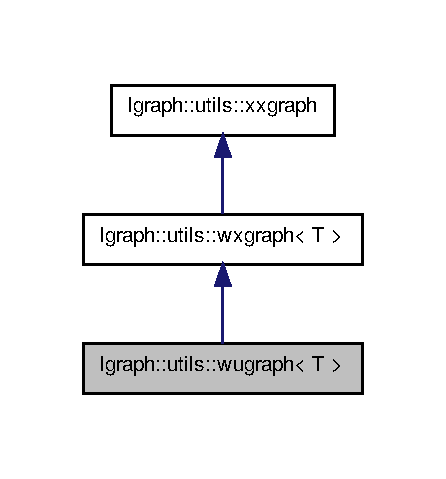
\includegraphics[width=214pt]{classlgraph_1_1utils_1_1wugraph__inherit__graph}
\end{center}
\end{figure}


Collaboration diagram for lgraph\+:\+:utils\+:\+:wugraph$<$ T $>$\+:\nopagebreak
\begin{figure}[H]
\begin{center}
\leavevmode
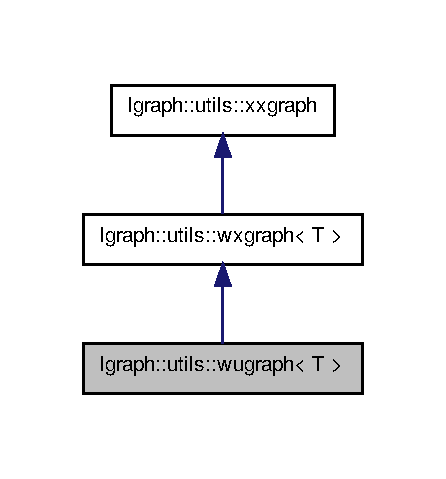
\includegraphics[width=214pt]{classlgraph_1_1utils_1_1wugraph__coll__graph}
\end{center}
\end{figure}
\subsection*{Public Member Functions}
\begin{DoxyCompactItemize}
\item 
\hyperlink{classlgraph_1_1utils_1_1wugraph_ae50a66b351ad581b460097ef43565cc2}{wugraph} ()\hypertarget{classlgraph_1_1utils_1_1wugraph_ae50a66b351ad581b460097ef43565cc2}{}\label{classlgraph_1_1utils_1_1wugraph_ae50a66b351ad581b460097ef43565cc2}

\begin{DoxyCompactList}\small\item\em Constructor. \end{DoxyCompactList}\item 
\hyperlink{classlgraph_1_1utils_1_1wugraph_a4e6ac08876defdc33d4ed8f5b1826384}{$\sim$wugraph} ()\hypertarget{classlgraph_1_1utils_1_1wugraph_a4e6ac08876defdc33d4ed8f5b1826384}{}\label{classlgraph_1_1utils_1_1wugraph_a4e6ac08876defdc33d4ed8f5b1826384}

\begin{DoxyCompactList}\small\item\em Destructor. \end{DoxyCompactList}\item 
void \hyperlink{classlgraph_1_1utils_1_1wugraph_a8e4db27ca594bc78cde948a7c9fa1f00}{add\+\_\+edge} (const \hyperlink{namespacelgraph_1_1utils_a6510284ce1b1ae5dc97ce5d2de426e10}{edge} \&e, const T \&w)
\begin{DoxyCompactList}\small\item\em Adds an edge to this graph. \end{DoxyCompactList}\item 
void \hyperlink{classlgraph_1_1utils_1_1wugraph_a64d5de79fb869156ba3a110a68d6ea3f}{add\+\_\+edge} (\hyperlink{namespacelgraph_1_1utils_ab9c6b34241f0b68372c55f34c460e863}{node} u, \hyperlink{namespacelgraph_1_1utils_ab9c6b34241f0b68372c55f34c460e863}{node} v, const T \&w)
\begin{DoxyCompactList}\small\item\em Adds an edge between nodes {\itshape u} and {\itshape v}. \end{DoxyCompactList}\item 
void \hyperlink{classlgraph_1_1utils_1_1wugraph_ad91246c2a9844d837ddb26e5abe563c6}{remove\+\_\+edge} (const \hyperlink{namespacelgraph_1_1utils_a6510284ce1b1ae5dc97ce5d2de426e10}{edge} \&e)
\begin{DoxyCompactList}\small\item\em Removes an edge from this graph. \end{DoxyCompactList}\item 
void \hyperlink{classlgraph_1_1utils_1_1wugraph_a8fd7f1a7ef76576a35e72687f4fdfce1}{remove\+\_\+edge} (\hyperlink{namespacelgraph_1_1utils_ab9c6b34241f0b68372c55f34c460e863}{node} u, \hyperlink{namespacelgraph_1_1utils_ab9c6b34241f0b68372c55f34c460e863}{node} v)
\begin{DoxyCompactList}\small\item\em Removes an edge from this graph. \end{DoxyCompactList}\item 
void \hyperlink{classlgraph_1_1utils_1_1wugraph_a877370aeb266c3fbe14f6ef890bff504}{edges} (vector$<$ pair$<$ \hyperlink{namespacelgraph_1_1utils_a6510284ce1b1ae5dc97ce5d2de426e10}{edge}, T $>$ $>$ \&all\+\_\+edges) const 
\begin{DoxyCompactList}\small\item\em Returns all unique edges of this graph. \end{DoxyCompactList}\item 
bool \hyperlink{classlgraph_1_1utils_1_1wugraph_a8c691c210f9b8f558f323f2aa187e5eb}{read\+\_\+from\+\_\+file} (const string \&filename)\hypertarget{classlgraph_1_1utils_1_1wugraph_a8c691c210f9b8f558f323f2aa187e5eb}{}\label{classlgraph_1_1utils_1_1wugraph_a8c691c210f9b8f558f323f2aa187e5eb}

\begin{DoxyCompactList}\small\item\em Reads the graph from a file. \end{DoxyCompactList}\item 
bool \hyperlink{classlgraph_1_1utils_1_1wugraph_afb7636ff2db2ff40a6f31a70dd599db1}{read\+\_\+from\+\_\+file} (const char $\ast$filename)\hypertarget{classlgraph_1_1utils_1_1wugraph_afb7636ff2db2ff40a6f31a70dd599db1}{}\label{classlgraph_1_1utils_1_1wugraph_afb7636ff2db2ff40a6f31a70dd599db1}

\begin{DoxyCompactList}\small\item\em Reads the graph from a file. \end{DoxyCompactList}\item 
bool \hyperlink{classlgraph_1_1utils_1_1wugraph_a824c084e6f4bf0e08f244ebccbf2d258}{store\+\_\+in\+\_\+file} (const string \&filename)\hypertarget{classlgraph_1_1utils_1_1wugraph_a824c084e6f4bf0e08f244ebccbf2d258}{}\label{classlgraph_1_1utils_1_1wugraph_a824c084e6f4bf0e08f244ebccbf2d258}

\begin{DoxyCompactList}\small\item\em Stores the graph in a file. \end{DoxyCompactList}\item 
bool \hyperlink{classlgraph_1_1utils_1_1wugraph_aab47f36e430b14c0d2181ed8e8399862}{store\+\_\+in\+\_\+file} (const char $\ast$filename)\hypertarget{classlgraph_1_1utils_1_1wugraph_aab47f36e430b14c0d2181ed8e8399862}{}\label{classlgraph_1_1utils_1_1wugraph_aab47f36e430b14c0d2181ed8e8399862}

\begin{DoxyCompactList}\small\item\em Stores the graph in a file. \end{DoxyCompactList}\item 
void \hyperlink{classlgraph_1_1utils_1_1wxgraph_a566ae9fe69209230ef159ed350ab8f7f}{init} (size\+\_\+t n)
\begin{DoxyCompactList}\small\item\em Initialises the attributes of a graph with {\itshape n} nodes. \end{DoxyCompactList}\item 
void \hyperlink{classlgraph_1_1utils_1_1wxgraph_a972a2483966f4b1d485c5d14157ee9be}{add\+\_\+edges} (const vector$<$ \hyperlink{namespacelgraph_1_1utils_a6510284ce1b1ae5dc97ce5d2de426e10}{edge} $>$ \&edge\+\_\+list, const vector$<$ T $>$ \&ws)
\begin{DoxyCompactList}\small\item\em Adds all edges taken from a list. \end{DoxyCompactList}\item 
void \hyperlink{classlgraph_1_1utils_1_1wxgraph_a4188b82f50e962b28c2c076b7978a854}{remove\+\_\+edges} (const vector$<$ \hyperlink{namespacelgraph_1_1utils_a6510284ce1b1ae5dc97ce5d2de426e10}{edge} $>$ \&edge\+\_\+list)
\begin{DoxyCompactList}\small\item\em Removes all edges taken from a list. \end{DoxyCompactList}\item 
void \hyperlink{classlgraph_1_1utils_1_1wxgraph_a421bc8166e35335445e45efc680ebe3f}{clear} ()
\begin{DoxyCompactList}\small\item\em Deletes all memory used by the graph. \end{DoxyCompactList}\item 
bool \hyperlink{classlgraph_1_1utils_1_1wxgraph_adda596cfbf72080d46ab445679fe092f}{is\+\_\+weighted} () const \hypertarget{classlgraph_1_1utils_1_1wxgraph_adda596cfbf72080d46ab445679fe092f}{}\label{classlgraph_1_1utils_1_1wxgraph_adda596cfbf72080d46ab445679fe092f}

\begin{DoxyCompactList}\small\item\em Returns whether this graph is weighted or not (returns true). \end{DoxyCompactList}\item 
T \hyperlink{classlgraph_1_1utils_1_1wxgraph_a1ec5455d64fb001903d3d0d1b5d8c7f2}{edge\+\_\+weight} (\hyperlink{namespacelgraph_1_1utils_ab9c6b34241f0b68372c55f34c460e863}{node} u, \hyperlink{namespacelgraph_1_1utils_ab9c6b34241f0b68372c55f34c460e863}{node} v) const 
\begin{DoxyCompactList}\small\item\em Returns the weight of the edge ({\itshape u}, {\itshape v}) \end{DoxyCompactList}\item 
const vector$<$ T $>$ \& \hyperlink{classlgraph_1_1utils_1_1wxgraph_ab52419fcc456987ee266104de356acc8}{get\+\_\+weights} (\hyperlink{namespacelgraph_1_1utils_ab9c6b34241f0b68372c55f34c460e863}{node} u) const 
\begin{DoxyCompactList}\small\item\em Returns a constant reference to all the weights of node {\itshape u}. \end{DoxyCompactList}\item 
void \hyperlink{classlgraph_1_1utils_1_1wxgraph_a36cc09578d49b326c3573b723536ea33}{get\+\_\+weights} (\hyperlink{namespacelgraph_1_1utils_ab9c6b34241f0b68372c55f34c460e863}{node} u, vector$<$ T $>$ \&ws) const 
\begin{DoxyCompactList}\small\item\em Returns the weights to all neighbours of node {\itshape u}. \end{DoxyCompactList}\item 
size\+\_\+t \hyperlink{classlgraph_1_1utils_1_1xxgraph_af41baf2c098e872731ad646aeec1b382}{add\+\_\+node} ()
\begin{DoxyCompactList}\small\item\em Adds one node to the graph. \end{DoxyCompactList}\item 
size\+\_\+t \hyperlink{classlgraph_1_1utils_1_1xxgraph_af4f3782c1a55f73c6f34f2f2c26fb404}{add\+\_\+n\+\_\+nodes} (\hyperlink{namespacelgraph_1_1utils_ab9c6b34241f0b68372c55f34c460e863}{node} n)
\begin{DoxyCompactList}\small\item\em Adds {\itshape n} nodes to the graph. \end{DoxyCompactList}\item 
bool \hyperlink{classlgraph_1_1utils_1_1xxgraph_a026ab064c2be26790cc1f547be2157c9}{has\+\_\+node} (\hyperlink{namespacelgraph_1_1utils_ab9c6b34241f0b68372c55f34c460e863}{node} u) const \hypertarget{classlgraph_1_1utils_1_1xxgraph_a026ab064c2be26790cc1f547be2157c9}{}\label{classlgraph_1_1utils_1_1xxgraph_a026ab064c2be26790cc1f547be2157c9}

\begin{DoxyCompactList}\small\item\em Returns true if node {\itshape u} is in this graph. \end{DoxyCompactList}\item 
bool \hyperlink{classlgraph_1_1utils_1_1xxgraph_a0bb7c5fc708596fff406cf3240ecd6b2}{has\+\_\+edge} (\hyperlink{namespacelgraph_1_1utils_ab9c6b34241f0b68372c55f34c460e863}{node} u, \hyperlink{namespacelgraph_1_1utils_ab9c6b34241f0b68372c55f34c460e863}{node} v) const 
\begin{DoxyCompactList}\small\item\em Returns true if there is an edge between nodes {\itshape u} and {\itshape v}. \end{DoxyCompactList}\item 
size\+\_\+t \hyperlink{classlgraph_1_1utils_1_1xxgraph_ad345f1fbf1dee34e1579b5aea9aef9b2}{n\+\_\+nodes} () const 
\begin{DoxyCompactList}\small\item\em Returns the number of nodes. \end{DoxyCompactList}\item 
size\+\_\+t \hyperlink{classlgraph_1_1utils_1_1xxgraph_af3f7c3835406c2cbf70479ae1c0253c9}{n\+\_\+edges} () const 
\begin{DoxyCompactList}\small\item\em Returns the number of edges. \end{DoxyCompactList}\item 
void \hyperlink{classlgraph_1_1utils_1_1xxgraph_a99f83387aa9f59b861e675251be5a3ad}{nodes} (vector$<$ \hyperlink{namespacelgraph_1_1utils_ab9c6b34241f0b68372c55f34c460e863}{node} $>$ \&all\+\_\+nodes) const \hypertarget{classlgraph_1_1utils_1_1xxgraph_a99f83387aa9f59b861e675251be5a3ad}{}\label{classlgraph_1_1utils_1_1xxgraph_a99f83387aa9f59b861e675251be5a3ad}

\begin{DoxyCompactList}\small\item\em Returns all nodes (as integers) \end{DoxyCompactList}\item 
const \hyperlink{namespacelgraph_1_1utils_a0f2ef47028a466d26841709e705390ac}{neighbourhood} \& \hyperlink{classlgraph_1_1utils_1_1xxgraph_a2c5332c4663c2d52828893f095a68202}{get\+\_\+neighbours} (\hyperlink{namespacelgraph_1_1utils_ab9c6b34241f0b68372c55f34c460e863}{node} u) const 
\begin{DoxyCompactList}\small\item\em Returns the neighbourhood of node u. \end{DoxyCompactList}\item 
size\+\_\+t \hyperlink{classlgraph_1_1utils_1_1xxgraph_af588aa4c68004a31aa143024cdb6dcc9}{degree} (\hyperlink{namespacelgraph_1_1utils_ab9c6b34241f0b68372c55f34c460e863}{node} u) const 
\begin{DoxyCompactList}\small\item\em Returns the number of neighbours of u. \end{DoxyCompactList}\item 
void \hyperlink{classlgraph_1_1utils_1_1xxgraph_a401454762f6b4b69f13ab0a10729c457}{get\+\_\+adjacency\+\_\+matrix} (vector$<$ vector$<$ bool $>$ $>$ \&adj\+\_\+mat) const \hypertarget{classlgraph_1_1utils_1_1xxgraph_a401454762f6b4b69f13ab0a10729c457}{}\label{classlgraph_1_1utils_1_1xxgraph_a401454762f6b4b69f13ab0a10729c457}

\begin{DoxyCompactList}\small\item\em Returns the adjacency matrix of this graph. \end{DoxyCompactList}\item 
void \hyperlink{classlgraph_1_1utils_1_1xxgraph_aff73f5ac4cd2732caa0c528eb1c1833c}{get\+\_\+degree\+\_\+sequence} (map$<$ size\+\_\+t, size\+\_\+t $>$ \&ds) const 
\begin{DoxyCompactList}\small\item\em Returns the degree sequence of the graph. \end{DoxyCompactList}\item 
size\+\_\+t \hyperlink{classlgraph_1_1utils_1_1xxgraph_ad4f25a8b29c6f26bc1567cb9c5a564ba}{n\+\_\+triangles} () const 
\begin{DoxyCompactList}\small\item\em Returns the number of triangles in this graph. \end{DoxyCompactList}\end{DoxyCompactItemize}
\subsection*{Protected Member Functions}
\begin{DoxyCompactItemize}
\item 
void \hyperlink{classlgraph_1_1utils_1_1wugraph_a365789840be9490091e6d8de03521cad}{get\+\_\+unique\+\_\+edges} (set$<$ pair$<$ \hyperlink{namespacelgraph_1_1utils_a6510284ce1b1ae5dc97ce5d2de426e10}{edge}, T $>$ $>$ \&\hyperlink{classlgraph_1_1utils_1_1wugraph_a877370aeb266c3fbe14f6ef890bff504}{edges}) const 
\begin{DoxyCompactList}\small\item\em Computes the list of unique weighted edges of this graph. \end{DoxyCompactList}\item 
void \hyperlink{classlgraph_1_1utils_1_1wxgraph_a0b0c0b54acbc7816eb5b9958e61805cf}{initialise\+\_\+weights} (size\+\_\+t n)\hypertarget{classlgraph_1_1utils_1_1wxgraph_a0b0c0b54acbc7816eb5b9958e61805cf}{}\label{classlgraph_1_1utils_1_1wxgraph_a0b0c0b54acbc7816eb5b9958e61805cf}

\begin{DoxyCompactList}\small\item\em Initialises the list of weights. \end{DoxyCompactList}\item 
void \hyperlink{classlgraph_1_1utils_1_1wxgraph_a145f81ae3609af5ec038ace8b4413fad}{clear\+\_\+weights} ()\hypertarget{classlgraph_1_1utils_1_1wxgraph_a145f81ae3609af5ec038ace8b4413fad}{}\label{classlgraph_1_1utils_1_1wxgraph_a145f81ae3609af5ec038ace8b4413fad}

\begin{DoxyCompactList}\small\item\em Clears the list of weights. \end{DoxyCompactList}\item 
\hyperlink{namespacelgraph_1_1utils_a7207b078932845778282f5e2e373575b}{ncit} \hyperlink{classlgraph_1_1utils_1_1xxgraph_af72476b0919eacd6e9b044f7c5528c1e}{cget\+\_\+neighbour\+\_\+position} (const \hyperlink{namespacelgraph_1_1utils_a0f2ef47028a466d26841709e705390ac}{neighbourhood} \&n, \hyperlink{namespacelgraph_1_1utils_ab9c6b34241f0b68372c55f34c460e863}{node} u) const 
\begin{DoxyCompactList}\small\item\em Returns a constant iterator to node {\itshape u\textquotesingle{}s} position in the neighbourhood {\itshape n}. \end{DoxyCompactList}\item 
\hyperlink{namespacelgraph_1_1utils_af5daf6fe356a9014746bdb507787ae01}{nit} \hyperlink{classlgraph_1_1utils_1_1xxgraph_ab2ac2eb4cdc6c369cde7c71a1c3b8858}{get\+\_\+neighbour\+\_\+position} (\hyperlink{namespacelgraph_1_1utils_a0f2ef47028a466d26841709e705390ac}{neighbourhood} \&n, \hyperlink{namespacelgraph_1_1utils_ab9c6b34241f0b68372c55f34c460e863}{node} u)
\begin{DoxyCompactList}\small\item\em Returns a non-\/constant iterator to node {\itshape u\textquotesingle{}s} position in the neighbourhood {\itshape n}. \end{DoxyCompactList}\item 
void \hyperlink{classlgraph_1_1utils_1_1xxgraph_a2201aaff5e9ffa29a9b3abfde705dd46}{initialise\+\_\+adjacency\+\_\+list} (size\+\_\+t n)\hypertarget{classlgraph_1_1utils_1_1xxgraph_a2201aaff5e9ffa29a9b3abfde705dd46}{}\label{classlgraph_1_1utils_1_1xxgraph_a2201aaff5e9ffa29a9b3abfde705dd46}

\begin{DoxyCompactList}\small\item\em Initialise the list of neighbourhoods with {\itshape n} instances. \end{DoxyCompactList}\item 
void \hyperlink{classlgraph_1_1utils_1_1xxgraph_a6523402d0ec66918b95de23d2bee38fc}{clear\+\_\+adjacency\+\_\+list} ()\hypertarget{classlgraph_1_1utils_1_1xxgraph_a6523402d0ec66918b95de23d2bee38fc}{}\label{classlgraph_1_1utils_1_1xxgraph_a6523402d0ec66918b95de23d2bee38fc}

\begin{DoxyCompactList}\small\item\em Clear the list of neighbourhoods. \end{DoxyCompactList}\item 
void \hyperlink{classlgraph_1_1utils_1_1xxgraph_abd983125be7f2f2b9c812326a4a39e6d}{initialise\+\_\+parent\+\_\+graph} (size\+\_\+t n)
\begin{DoxyCompactList}\small\item\em Initialises the adjacency list of this graph. \end{DoxyCompactList}\item 
void \hyperlink{classlgraph_1_1utils_1_1xxgraph_a8d213a8dfe716d344dd51d1bd37c0e2c}{clear\+\_\+parent\+\_\+graph} ()
\begin{DoxyCompactList}\small\item\em Clears the adjacency list of this graph. \end{DoxyCompactList}\end{DoxyCompactItemize}
\subsection*{Protected Attributes}
\begin{DoxyCompactItemize}
\item 
vector$<$ \hyperlink{namespacelgraph_1_1utils_a11e7963f3637ea13778b8d3e69d2c17f}{weight\+\_\+list}$<$ T $>$ $>$ \hyperlink{classlgraph_1_1utils_1_1wxgraph_a15569c8c0fccb641709dc81eb0e29c94}{weights}
\begin{DoxyCompactList}\small\item\em Weight list for each node. \end{DoxyCompactList}\item 
vector$<$ \hyperlink{namespacelgraph_1_1utils_a0f2ef47028a466d26841709e705390ac}{neighbourhood} $>$ \hyperlink{classlgraph_1_1utils_1_1xxgraph_a1d5fda0d5aa89340f997428b982f966f}{adjacency\+\_\+list}\hypertarget{classlgraph_1_1utils_1_1xxgraph_a1d5fda0d5aa89340f997428b982f966f}{}\label{classlgraph_1_1utils_1_1xxgraph_a1d5fda0d5aa89340f997428b982f966f}

\begin{DoxyCompactList}\small\item\em The neighbourhood of every node. \end{DoxyCompactList}\item 
size\+\_\+t \hyperlink{classlgraph_1_1utils_1_1xxgraph_a217ebb1cd8946fedfbf94a9b22f7da48}{num\+\_\+edges}\hypertarget{classlgraph_1_1utils_1_1xxgraph_a217ebb1cd8946fedfbf94a9b22f7da48}{}\label{classlgraph_1_1utils_1_1xxgraph_a217ebb1cd8946fedfbf94a9b22f7da48}

\begin{DoxyCompactList}\small\item\em The amount of edges in this graph. \end{DoxyCompactList}\end{DoxyCompactItemize}


\subsection{Detailed Description}
\subsubsection*{template$<$class T$>$\\*
class lgraph\+::utils\+::wugraph$<$ T $>$}

Weighted undirected graphs. 

This class implements the weighted, undirected graph data structure based on adjacency lists.


\begin{DoxyParams}{Parameters}
{\em T} & In case of weighted graphs, this parameter indicates the type of the edge weights \\
\hline
\end{DoxyParams}


\subsection{Member Function Documentation}
\index{lgraph\+::utils\+::wugraph@{lgraph\+::utils\+::wugraph}!add\+\_\+edge@{add\+\_\+edge}}
\index{add\+\_\+edge@{add\+\_\+edge}!lgraph\+::utils\+::wugraph@{lgraph\+::utils\+::wugraph}}
\subsubsection[{\texorpdfstring{add\+\_\+edge(const edge \&e, const T \&w)}{add_edge(const edge &e, const T &w)}}]{\setlength{\rightskip}{0pt plus 5cm}template$<$class T $>$ void {\bf lgraph\+::utils\+::wugraph}$<$ T $>$\+::add\+\_\+edge (
\begin{DoxyParamCaption}
\item[{const {\bf edge} \&}]{e, }
\item[{const T \&}]{w}
\end{DoxyParamCaption}
)\hspace{0.3cm}{\ttfamily [virtual]}}\hypertarget{classlgraph_1_1utils_1_1wugraph_a8e4db27ca594bc78cde948a7c9fa1f00}{}\label{classlgraph_1_1utils_1_1wugraph_a8e4db27ca594bc78cde948a7c9fa1f00}


Adds an edge to this graph. 

The attribute \hyperlink{classlgraph_1_1utils_1_1xxgraph_a217ebb1cd8946fedfbf94a9b22f7da48}{num\+\_\+edges} is incremented by one. 
\begin{DoxyParams}{Parameters}
{\em e} & A pair of nodes \\
\hline
{\em w} & The weight of the edge \\
\hline
\end{DoxyParams}


Implements \hyperlink{classlgraph_1_1utils_1_1wxgraph_a8bee4a49537954adf70d720e0677caee}{lgraph\+::utils\+::wxgraph$<$ T $>$}.

\index{lgraph\+::utils\+::wugraph@{lgraph\+::utils\+::wugraph}!add\+\_\+edge@{add\+\_\+edge}}
\index{add\+\_\+edge@{add\+\_\+edge}!lgraph\+::utils\+::wugraph@{lgraph\+::utils\+::wugraph}}
\subsubsection[{\texorpdfstring{add\+\_\+edge(node u, node v, const T \&w)}{add_edge(node u, node v, const T &w)}}]{\setlength{\rightskip}{0pt plus 5cm}template$<$class T $>$ void {\bf lgraph\+::utils\+::wugraph}$<$ T $>$\+::add\+\_\+edge (
\begin{DoxyParamCaption}
\item[{{\bf node}}]{u, }
\item[{{\bf node}}]{v, }
\item[{const T \&}]{w}
\end{DoxyParamCaption}
)\hspace{0.3cm}{\ttfamily [virtual]}}\hypertarget{classlgraph_1_1utils_1_1wugraph_a64d5de79fb869156ba3a110a68d6ea3f}{}\label{classlgraph_1_1utils_1_1wugraph_a64d5de79fb869156ba3a110a68d6ea3f}


Adds an edge between nodes {\itshape u} and {\itshape v}. 

The attribute \hyperlink{classlgraph_1_1utils_1_1xxgraph_a217ebb1cd8946fedfbf94a9b22f7da48}{num\+\_\+edges} is incremented by one.


\begin{DoxyParams}{Parameters}
{\em u} & The fist node of the edge \\
\hline
{\em v} & The second node of the edge \\
\hline
{\em w} & The weight of the edge \\
\hline
\end{DoxyParams}


Implements \hyperlink{classlgraph_1_1utils_1_1wxgraph_a2cc33d25e8e593fa48cc05fdf0e96f9f}{lgraph\+::utils\+::wxgraph$<$ T $>$}.

\index{lgraph\+::utils\+::wugraph@{lgraph\+::utils\+::wugraph}!add\+\_\+edges@{add\+\_\+edges}}
\index{add\+\_\+edges@{add\+\_\+edges}!lgraph\+::utils\+::wugraph@{lgraph\+::utils\+::wugraph}}
\subsubsection[{\texorpdfstring{add\+\_\+edges(const vector$<$ edge $>$ \&edge\+\_\+list, const vector$<$ T $>$ \&ws)}{add_edges(const vector< edge > &edge_list, const vector< T > &ws)}}]{\setlength{\rightskip}{0pt plus 5cm}template$<$class T $>$ void {\bf lgraph\+::utils\+::wxgraph}$<$ T $>$\+::add\+\_\+edges (
\begin{DoxyParamCaption}
\item[{const vector$<$ {\bf edge} $>$ \&}]{edge\+\_\+list, }
\item[{const vector$<$ T $>$ \&}]{ws}
\end{DoxyParamCaption}
)\hspace{0.3cm}{\ttfamily [inherited]}}\hypertarget{classlgraph_1_1utils_1_1wxgraph_a972a2483966f4b1d485c5d14157ee9be}{}\label{classlgraph_1_1utils_1_1wxgraph_a972a2483966f4b1d485c5d14157ee9be}


Adds all edges taken from a list. 

The attribute \hyperlink{classlgraph_1_1utils_1_1xxgraph_a217ebb1cd8946fedfbf94a9b22f7da48}{num\+\_\+edges} is incremented as many times as elements there are in {\itshape edge\+\_\+list}. 
\begin{DoxyParams}{Parameters}
{\em edge\+\_\+list} & A list of pairs of nodes \\
\hline
{\em ws} & A list of weights. The i-\/th edge has weight {\itshape ws}\mbox{[}i\mbox{]}. \\
\hline
\end{DoxyParams}
\index{lgraph\+::utils\+::wugraph@{lgraph\+::utils\+::wugraph}!add\+\_\+n\+\_\+nodes@{add\+\_\+n\+\_\+nodes}}
\index{add\+\_\+n\+\_\+nodes@{add\+\_\+n\+\_\+nodes}!lgraph\+::utils\+::wugraph@{lgraph\+::utils\+::wugraph}}
\subsubsection[{\texorpdfstring{add\+\_\+n\+\_\+nodes(node n)}{add_n_nodes(node n)}}]{\setlength{\rightskip}{0pt plus 5cm}size\+\_\+t lgraph\+::utils\+::xxgraph\+::add\+\_\+n\+\_\+nodes (
\begin{DoxyParamCaption}
\item[{{\bf node}}]{n}
\end{DoxyParamCaption}
)\hspace{0.3cm}{\ttfamily [inherited]}}\hypertarget{classlgraph_1_1utils_1_1xxgraph_af4f3782c1a55f73c6f34f2f2c26fb404}{}\label{classlgraph_1_1utils_1_1xxgraph_af4f3782c1a55f73c6f34f2f2c26fb404}


Adds {\itshape n} nodes to the graph. 

The nodes are assigned consecutive, increasing values. \begin{DoxyReturn}{Returns}
Returns the index of the last node. 
\end{DoxyReturn}
\index{lgraph\+::utils\+::wugraph@{lgraph\+::utils\+::wugraph}!add\+\_\+node@{add\+\_\+node}}
\index{add\+\_\+node@{add\+\_\+node}!lgraph\+::utils\+::wugraph@{lgraph\+::utils\+::wugraph}}
\subsubsection[{\texorpdfstring{add\+\_\+node()}{add_node()}}]{\setlength{\rightskip}{0pt plus 5cm}size\+\_\+t lgraph\+::utils\+::xxgraph\+::add\+\_\+node (
\begin{DoxyParamCaption}
{}
\end{DoxyParamCaption}
)\hspace{0.3cm}{\ttfamily [inherited]}}\hypertarget{classlgraph_1_1utils_1_1xxgraph_af41baf2c098e872731ad646aeec1b382}{}\label{classlgraph_1_1utils_1_1xxgraph_af41baf2c098e872731ad646aeec1b382}


Adds one node to the graph. 

\begin{DoxyReturn}{Returns}
Returns the index of the new node 
\end{DoxyReturn}
\index{lgraph\+::utils\+::wugraph@{lgraph\+::utils\+::wugraph}!cget\+\_\+neighbour\+\_\+position@{cget\+\_\+neighbour\+\_\+position}}
\index{cget\+\_\+neighbour\+\_\+position@{cget\+\_\+neighbour\+\_\+position}!lgraph\+::utils\+::wugraph@{lgraph\+::utils\+::wugraph}}
\subsubsection[{\texorpdfstring{cget\+\_\+neighbour\+\_\+position(const neighbourhood \&n, node u) const }{cget_neighbour_position(const neighbourhood &n, node u) const }}]{\setlength{\rightskip}{0pt plus 5cm}{\bf ncit} lgraph\+::utils\+::xxgraph\+::cget\+\_\+neighbour\+\_\+position (
\begin{DoxyParamCaption}
\item[{const {\bf neighbourhood} \&}]{n, }
\item[{{\bf node}}]{u}
\end{DoxyParamCaption}
) const\hspace{0.3cm}{\ttfamily [protected]}, {\ttfamily [inherited]}}\hypertarget{classlgraph_1_1utils_1_1xxgraph_af72476b0919eacd6e9b044f7c5528c1e}{}\label{classlgraph_1_1utils_1_1xxgraph_af72476b0919eacd6e9b044f7c5528c1e}


Returns a constant iterator to node {\itshape u\textquotesingle{}s} position in the neighbourhood {\itshape n}. 

If the iterator returned is not at the end of the list then {\itshape u} is in the list. Performs a linear search to find it. 
\begin{DoxyParams}{Parameters}
{\em n} & The neighbourhood of a node in the graph \\
\hline
{\em u} & The node to look for in the neighbourhood \\
\hline
\end{DoxyParams}
\begin{DoxyReturn}{Returns}
Returns a constant iterator to {\itshape n.\+end()} if {\itshape u} is not in the list. Returns a constant iterator to the position of {\itshape u} if otherwise. 
\end{DoxyReturn}
\index{lgraph\+::utils\+::wugraph@{lgraph\+::utils\+::wugraph}!clear@{clear}}
\index{clear@{clear}!lgraph\+::utils\+::wugraph@{lgraph\+::utils\+::wugraph}}
\subsubsection[{\texorpdfstring{clear()}{clear()}}]{\setlength{\rightskip}{0pt plus 5cm}template$<$class T $>$ void {\bf lgraph\+::utils\+::wxgraph}$<$ T $>$\+::clear (
\begin{DoxyParamCaption}
{}
\end{DoxyParamCaption}
)\hspace{0.3cm}{\ttfamily [inherited]}}\hypertarget{classlgraph_1_1utils_1_1wxgraph_a421bc8166e35335445e45efc680ebe3f}{}\label{classlgraph_1_1utils_1_1wxgraph_a421bc8166e35335445e45efc680ebe3f}


Deletes all memory used by the graph. 

The value \hyperlink{classlgraph_1_1utils_1_1xxgraph_a217ebb1cd8946fedfbf94a9b22f7da48}{num\+\_\+edges} is set to 0. \index{lgraph\+::utils\+::wugraph@{lgraph\+::utils\+::wugraph}!clear\+\_\+parent\+\_\+graph@{clear\+\_\+parent\+\_\+graph}}
\index{clear\+\_\+parent\+\_\+graph@{clear\+\_\+parent\+\_\+graph}!lgraph\+::utils\+::wugraph@{lgraph\+::utils\+::wugraph}}
\subsubsection[{\texorpdfstring{clear\+\_\+parent\+\_\+graph()}{clear_parent_graph()}}]{\setlength{\rightskip}{0pt plus 5cm}void lgraph\+::utils\+::xxgraph\+::clear\+\_\+parent\+\_\+graph (
\begin{DoxyParamCaption}
{}
\end{DoxyParamCaption}
)\hspace{0.3cm}{\ttfamily [protected]}, {\ttfamily [inherited]}}\hypertarget{classlgraph_1_1utils_1_1xxgraph_a8d213a8dfe716d344dd51d1bd37c0e2c}{}\label{classlgraph_1_1utils_1_1xxgraph_a8d213a8dfe716d344dd51d1bd37c0e2c}


Clears the adjacency list of this graph. 

The value \hyperlink{classlgraph_1_1utils_1_1xxgraph_a217ebb1cd8946fedfbf94a9b22f7da48}{num\+\_\+edges} is set to 0. \index{lgraph\+::utils\+::wugraph@{lgraph\+::utils\+::wugraph}!degree@{degree}}
\index{degree@{degree}!lgraph\+::utils\+::wugraph@{lgraph\+::utils\+::wugraph}}
\subsubsection[{\texorpdfstring{degree(node u) const }{degree(node u) const }}]{\setlength{\rightskip}{0pt plus 5cm}size\+\_\+t lgraph\+::utils\+::xxgraph\+::degree (
\begin{DoxyParamCaption}
\item[{{\bf node}}]{u}
\end{DoxyParamCaption}
) const\hspace{0.3cm}{\ttfamily [inherited]}}\hypertarget{classlgraph_1_1utils_1_1xxgraph_af588aa4c68004a31aa143024cdb6dcc9}{}\label{classlgraph_1_1utils_1_1xxgraph_af588aa4c68004a31aa143024cdb6dcc9}


Returns the number of neighbours of u. 


\begin{DoxyParams}{Parameters}
{\em u} & The node whose neighbourhood size we want \\
\hline
\end{DoxyParams}
\begin{DoxyReturn}{Returns}
Returns the size of the neighbourhood of {\itshape u}, that is, the size of the list in \hyperlink{classlgraph_1_1utils_1_1xxgraph_a1d5fda0d5aa89340f997428b982f966f}{adjacency\+\_\+list}\mbox{[}u\mbox{]} 
\end{DoxyReturn}
\begin{DoxyPrecond}{Precondition}
{\itshape u} must be a node from the graph 
\end{DoxyPrecond}
\index{lgraph\+::utils\+::wugraph@{lgraph\+::utils\+::wugraph}!edge\+\_\+weight@{edge\+\_\+weight}}
\index{edge\+\_\+weight@{edge\+\_\+weight}!lgraph\+::utils\+::wugraph@{lgraph\+::utils\+::wugraph}}
\subsubsection[{\texorpdfstring{edge\+\_\+weight(node u, node v) const }{edge_weight(node u, node v) const }}]{\setlength{\rightskip}{0pt plus 5cm}template$<$class T $>$ T {\bf lgraph\+::utils\+::wxgraph}$<$ T $>$\+::edge\+\_\+weight (
\begin{DoxyParamCaption}
\item[{{\bf node}}]{u, }
\item[{{\bf node}}]{v}
\end{DoxyParamCaption}
) const\hspace{0.3cm}{\ttfamily [inherited]}}\hypertarget{classlgraph_1_1utils_1_1wxgraph_a1ec5455d64fb001903d3d0d1b5d8c7f2}{}\label{classlgraph_1_1utils_1_1wxgraph_a1ec5455d64fb001903d3d0d1b5d8c7f2}


Returns the weight of the edge ({\itshape u}, {\itshape v}) 

\begin{DoxyPrecond}{Precondition}
The edge ({\itshape u}, {\itshape v}) must be in the graph 
\end{DoxyPrecond}
\index{lgraph\+::utils\+::wugraph@{lgraph\+::utils\+::wugraph}!edges@{edges}}
\index{edges@{edges}!lgraph\+::utils\+::wugraph@{lgraph\+::utils\+::wugraph}}
\subsubsection[{\texorpdfstring{edges(vector$<$ pair$<$ edge, T $>$ $>$ \&all\+\_\+edges) const }{edges(vector< pair< edge, T > > &all_edges) const }}]{\setlength{\rightskip}{0pt plus 5cm}template$<$class T $>$ void {\bf lgraph\+::utils\+::wugraph}$<$ T $>$\+::edges (
\begin{DoxyParamCaption}
\item[{vector$<$ pair$<$ {\bf edge}, T $>$ $>$ \&}]{all\+\_\+edges}
\end{DoxyParamCaption}
) const\hspace{0.3cm}{\ttfamily [virtual]}}\hypertarget{classlgraph_1_1utils_1_1wugraph_a877370aeb266c3fbe14f6ef890bff504}{}\label{classlgraph_1_1utils_1_1wugraph_a877370aeb266c3fbe14f6ef890bff504}


Returns all unique edges of this graph. 

See method \hyperlink{classlgraph_1_1utils_1_1wugraph_a365789840be9490091e6d8de03521cad}{get\+\_\+unique\+\_\+edges(set$<$pair$<$edge,\+T$>$ $>$\& edges)const} for details. 

Implements \hyperlink{classlgraph_1_1utils_1_1wxgraph_acbe42102887d02b8942ee4657573581f}{lgraph\+::utils\+::wxgraph$<$ T $>$}.

\index{lgraph\+::utils\+::wugraph@{lgraph\+::utils\+::wugraph}!get\+\_\+degree\+\_\+sequence@{get\+\_\+degree\+\_\+sequence}}
\index{get\+\_\+degree\+\_\+sequence@{get\+\_\+degree\+\_\+sequence}!lgraph\+::utils\+::wugraph@{lgraph\+::utils\+::wugraph}}
\subsubsection[{\texorpdfstring{get\+\_\+degree\+\_\+sequence(map$<$ size\+\_\+t, size\+\_\+t $>$ \&ds) const }{get_degree_sequence(map< size_t, size_t > &ds) const }}]{\setlength{\rightskip}{0pt plus 5cm}void lgraph\+::utils\+::xxgraph\+::get\+\_\+degree\+\_\+sequence (
\begin{DoxyParamCaption}
\item[{map$<$ size\+\_\+t, size\+\_\+t $>$ \&}]{ds}
\end{DoxyParamCaption}
) const\hspace{0.3cm}{\ttfamily [inherited]}}\hypertarget{classlgraph_1_1utils_1_1xxgraph_aff73f5ac4cd2732caa0c528eb1c1833c}{}\label{classlgraph_1_1utils_1_1xxgraph_aff73f5ac4cd2732caa0c528eb1c1833c}


Returns the degree sequence of the graph. 


\begin{DoxyParams}[1]{Parameters}
\mbox{\tt out}  & {\em ds} & A list of pairs\+: for each degree the amount of nodes in this graph that have that degree. The degree of a node is detailed in \hyperlink{classlgraph_1_1utils_1_1xxgraph_af588aa4c68004a31aa143024cdb6dcc9}{degree} \\
\hline
\end{DoxyParams}
\index{lgraph\+::utils\+::wugraph@{lgraph\+::utils\+::wugraph}!get\+\_\+neighbour\+\_\+position@{get\+\_\+neighbour\+\_\+position}}
\index{get\+\_\+neighbour\+\_\+position@{get\+\_\+neighbour\+\_\+position}!lgraph\+::utils\+::wugraph@{lgraph\+::utils\+::wugraph}}
\subsubsection[{\texorpdfstring{get\+\_\+neighbour\+\_\+position(neighbourhood \&n, node u)}{get_neighbour_position(neighbourhood &n, node u)}}]{\setlength{\rightskip}{0pt plus 5cm}{\bf nit} lgraph\+::utils\+::xxgraph\+::get\+\_\+neighbour\+\_\+position (
\begin{DoxyParamCaption}
\item[{{\bf neighbourhood} \&}]{n, }
\item[{{\bf node}}]{u}
\end{DoxyParamCaption}
)\hspace{0.3cm}{\ttfamily [protected]}, {\ttfamily [inherited]}}\hypertarget{classlgraph_1_1utils_1_1xxgraph_ab2ac2eb4cdc6c369cde7c71a1c3b8858}{}\label{classlgraph_1_1utils_1_1xxgraph_ab2ac2eb4cdc6c369cde7c71a1c3b8858}


Returns a non-\/constant iterator to node {\itshape u\textquotesingle{}s} position in the neighbourhood {\itshape n}. 

If the iterator returned is not at the end of the list then {\itshape u} is in the list. Performs a linear search to find it. 
\begin{DoxyParams}{Parameters}
{\em n} & The neighbourhood of a node in the graph \\
\hline
{\em u} & The node to look for in the neighbourhood \\
\hline
\end{DoxyParams}
\begin{DoxyReturn}{Returns}
Returns a non-\/constant iterator to {\itshape n.\+end()} if {\itshape u} is not in the list. Returns a non-\/constant iterator to the position of {\itshape u} if otherwise. 
\end{DoxyReturn}
\index{lgraph\+::utils\+::wugraph@{lgraph\+::utils\+::wugraph}!get\+\_\+neighbours@{get\+\_\+neighbours}}
\index{get\+\_\+neighbours@{get\+\_\+neighbours}!lgraph\+::utils\+::wugraph@{lgraph\+::utils\+::wugraph}}
\subsubsection[{\texorpdfstring{get\+\_\+neighbours(node u) const }{get_neighbours(node u) const }}]{\setlength{\rightskip}{0pt plus 5cm}const {\bf neighbourhood} \& lgraph\+::utils\+::xxgraph\+::get\+\_\+neighbours (
\begin{DoxyParamCaption}
\item[{{\bf node}}]{u}
\end{DoxyParamCaption}
) const\hspace{0.3cm}{\ttfamily [inherited]}}\hypertarget{classlgraph_1_1utils_1_1xxgraph_a2c5332c4663c2d52828893f095a68202}{}\label{classlgraph_1_1utils_1_1xxgraph_a2c5332c4663c2d52828893f095a68202}


Returns the neighbourhood of node u. 


\begin{DoxyParams}{Parameters}
{\em u} & The node whose neighbourhood we want \\
\hline
\end{DoxyParams}
\begin{DoxyPrecond}{Precondition}
{\itshape u} must be a node from the graph 
\end{DoxyPrecond}
\index{lgraph\+::utils\+::wugraph@{lgraph\+::utils\+::wugraph}!get\+\_\+unique\+\_\+edges@{get\+\_\+unique\+\_\+edges}}
\index{get\+\_\+unique\+\_\+edges@{get\+\_\+unique\+\_\+edges}!lgraph\+::utils\+::wugraph@{lgraph\+::utils\+::wugraph}}
\subsubsection[{\texorpdfstring{get\+\_\+unique\+\_\+edges(set$<$ pair$<$ edge, T $>$ $>$ \&edges) const }{get_unique_edges(set< pair< edge, T > > &edges) const }}]{\setlength{\rightskip}{0pt plus 5cm}template$<$class T $>$ void {\bf lgraph\+::utils\+::wugraph}$<$ T $>$\+::get\+\_\+unique\+\_\+edges (
\begin{DoxyParamCaption}
\item[{set$<$ pair$<$ {\bf edge}, T $>$ $>$ \&}]{edges}
\end{DoxyParamCaption}
) const\hspace{0.3cm}{\ttfamily [protected]}, {\ttfamily [virtual]}}\hypertarget{classlgraph_1_1utils_1_1wugraph_a365789840be9490091e6d8de03521cad}{}\label{classlgraph_1_1utils_1_1wugraph_a365789840be9490091e6d8de03521cad}


Computes the list of unique weighted edges of this graph. 

Since this graph is undirected, the edge (u,v) is the same as (v,u). This method computes the list of edges so that the result is lexicographically sorted. A weighted edge is a pair of two elements\+: an edge (a pair of two indices) and a weight. Each index is within the interval \mbox{[}0,{\itshape n}) where {\itshape n} is the number of nodes of this graph.


\begin{DoxyParams}[1]{Parameters}
\mbox{\tt out}  & {\em edges} & The collection of weighted edges \\
\hline
\end{DoxyParams}
\begin{DoxyReturn}{Returns}
Stores in \hyperlink{classlgraph_1_1utils_1_1wugraph_a877370aeb266c3fbe14f6ef890bff504}{edges} the lexicographically sorted list of weighted edges of this graph 
\end{DoxyReturn}


Implements \hyperlink{classlgraph_1_1utils_1_1wxgraph_ae49fda28107ce983b8f0d641468e9a75}{lgraph\+::utils\+::wxgraph$<$ T $>$}.

\index{lgraph\+::utils\+::wugraph@{lgraph\+::utils\+::wugraph}!get\+\_\+weights@{get\+\_\+weights}}
\index{get\+\_\+weights@{get\+\_\+weights}!lgraph\+::utils\+::wugraph@{lgraph\+::utils\+::wugraph}}
\subsubsection[{\texorpdfstring{get\+\_\+weights(node u) const }{get_weights(node u) const }}]{\setlength{\rightskip}{0pt plus 5cm}template$<$class T $>$ const vector$<$ T $>$ \& {\bf lgraph\+::utils\+::wxgraph}$<$ T $>$\+::get\+\_\+weights (
\begin{DoxyParamCaption}
\item[{{\bf node}}]{u}
\end{DoxyParamCaption}
) const\hspace{0.3cm}{\ttfamily [inherited]}}\hypertarget{classlgraph_1_1utils_1_1wxgraph_ab52419fcc456987ee266104de356acc8}{}\label{classlgraph_1_1utils_1_1wxgraph_ab52419fcc456987ee266104de356acc8}


Returns a constant reference to all the weights of node {\itshape u}. 


\begin{DoxyParams}{Parameters}
{\em u} & The node whose weight list is requested \\
\hline
\end{DoxyParams}
\begin{DoxyReturn}{Returns}
The weight list of node {\itshape u} 
\end{DoxyReturn}
\index{lgraph\+::utils\+::wugraph@{lgraph\+::utils\+::wugraph}!get\+\_\+weights@{get\+\_\+weights}}
\index{get\+\_\+weights@{get\+\_\+weights}!lgraph\+::utils\+::wugraph@{lgraph\+::utils\+::wugraph}}
\subsubsection[{\texorpdfstring{get\+\_\+weights(node u, vector$<$ T $>$ \&ws) const }{get_weights(node u, vector< T > &ws) const }}]{\setlength{\rightskip}{0pt plus 5cm}template$<$class T $>$ void {\bf lgraph\+::utils\+::wxgraph}$<$ T $>$\+::get\+\_\+weights (
\begin{DoxyParamCaption}
\item[{{\bf node}}]{u, }
\item[{vector$<$ T $>$ \&}]{ws}
\end{DoxyParamCaption}
) const\hspace{0.3cm}{\ttfamily [inherited]}}\hypertarget{classlgraph_1_1utils_1_1wxgraph_a36cc09578d49b326c3573b723536ea33}{}\label{classlgraph_1_1utils_1_1wxgraph_a36cc09578d49b326c3573b723536ea33}


Returns the weights to all neighbours of node {\itshape u}. 

\begin{DoxyPrecond}{Precondition}
{\itshape u} must be in the graph 
\end{DoxyPrecond}
\index{lgraph\+::utils\+::wugraph@{lgraph\+::utils\+::wugraph}!has\+\_\+edge@{has\+\_\+edge}}
\index{has\+\_\+edge@{has\+\_\+edge}!lgraph\+::utils\+::wugraph@{lgraph\+::utils\+::wugraph}}
\subsubsection[{\texorpdfstring{has\+\_\+edge(node u, node v) const }{has_edge(node u, node v) const }}]{\setlength{\rightskip}{0pt plus 5cm}bool lgraph\+::utils\+::xxgraph\+::has\+\_\+edge (
\begin{DoxyParamCaption}
\item[{{\bf node}}]{u, }
\item[{{\bf node}}]{v}
\end{DoxyParamCaption}
) const\hspace{0.3cm}{\ttfamily [inherited]}}\hypertarget{classlgraph_1_1utils_1_1xxgraph_a0bb7c5fc708596fff406cf3240ecd6b2}{}\label{classlgraph_1_1utils_1_1xxgraph_a0bb7c5fc708596fff406cf3240ecd6b2}


Returns true if there is an edge between nodes {\itshape u} and {\itshape v}. 

\begin{DoxyPrecond}{Precondition}
{\itshape u} and {\itshape v} must be in the graph 
\end{DoxyPrecond}
\index{lgraph\+::utils\+::wugraph@{lgraph\+::utils\+::wugraph}!init@{init}}
\index{init@{init}!lgraph\+::utils\+::wugraph@{lgraph\+::utils\+::wugraph}}
\subsubsection[{\texorpdfstring{init(size\+\_\+t n)}{init(size_t n)}}]{\setlength{\rightskip}{0pt plus 5cm}template$<$class T $>$ void {\bf lgraph\+::utils\+::wxgraph}$<$ T $>$\+::init (
\begin{DoxyParamCaption}
\item[{size\+\_\+t}]{n}
\end{DoxyParamCaption}
)\hspace{0.3cm}{\ttfamily [virtual]}, {\ttfamily [inherited]}}\hypertarget{classlgraph_1_1utils_1_1wxgraph_a566ae9fe69209230ef159ed350ab8f7f}{}\label{classlgraph_1_1utils_1_1wxgraph_a566ae9fe69209230ef159ed350ab8f7f}


Initialises the attributes of a graph with {\itshape n} nodes. 

First, it clears all the memory allocated so far. Then, initialises all the attributes so that it can store all the necessary information. 
\begin{DoxyParams}{Parameters}
{\em n} & Number of nodes of the graph \\
\hline
\end{DoxyParams}


Implements \hyperlink{classlgraph_1_1utils_1_1xxgraph_a2ac8b3e71fa0550248c692a19ea04d0d}{lgraph\+::utils\+::xxgraph}.

\index{lgraph\+::utils\+::wugraph@{lgraph\+::utils\+::wugraph}!initialise\+\_\+parent\+\_\+graph@{initialise\+\_\+parent\+\_\+graph}}
\index{initialise\+\_\+parent\+\_\+graph@{initialise\+\_\+parent\+\_\+graph}!lgraph\+::utils\+::wugraph@{lgraph\+::utils\+::wugraph}}
\subsubsection[{\texorpdfstring{initialise\+\_\+parent\+\_\+graph(size\+\_\+t n)}{initialise_parent_graph(size_t n)}}]{\setlength{\rightskip}{0pt plus 5cm}void lgraph\+::utils\+::xxgraph\+::initialise\+\_\+parent\+\_\+graph (
\begin{DoxyParamCaption}
\item[{size\+\_\+t}]{n}
\end{DoxyParamCaption}
)\hspace{0.3cm}{\ttfamily [protected]}, {\ttfamily [inherited]}}\hypertarget{classlgraph_1_1utils_1_1xxgraph_abd983125be7f2f2b9c812326a4a39e6d}{}\label{classlgraph_1_1utils_1_1xxgraph_abd983125be7f2f2b9c812326a4a39e6d}


Initialises the adjacency list of this graph. 

The value \hyperlink{classlgraph_1_1utils_1_1xxgraph_a217ebb1cd8946fedfbf94a9b22f7da48}{num\+\_\+edges} is set to 0. \index{lgraph\+::utils\+::wugraph@{lgraph\+::utils\+::wugraph}!n\+\_\+edges@{n\+\_\+edges}}
\index{n\+\_\+edges@{n\+\_\+edges}!lgraph\+::utils\+::wugraph@{lgraph\+::utils\+::wugraph}}
\subsubsection[{\texorpdfstring{n\+\_\+edges() const }{n_edges() const }}]{\setlength{\rightskip}{0pt plus 5cm}size\+\_\+t lgraph\+::utils\+::xxgraph\+::n\+\_\+edges (
\begin{DoxyParamCaption}
{}
\end{DoxyParamCaption}
) const\hspace{0.3cm}{\ttfamily [inherited]}}\hypertarget{classlgraph_1_1utils_1_1xxgraph_af3f7c3835406c2cbf70479ae1c0253c9}{}\label{classlgraph_1_1utils_1_1xxgraph_af3f7c3835406c2cbf70479ae1c0253c9}


Returns the number of edges. 

\begin{DoxyReturn}{Returns}
Returns the value \hyperlink{classlgraph_1_1utils_1_1xxgraph_a217ebb1cd8946fedfbf94a9b22f7da48}{num\+\_\+edges} 
\end{DoxyReturn}
\index{lgraph\+::utils\+::wugraph@{lgraph\+::utils\+::wugraph}!n\+\_\+nodes@{n\+\_\+nodes}}
\index{n\+\_\+nodes@{n\+\_\+nodes}!lgraph\+::utils\+::wugraph@{lgraph\+::utils\+::wugraph}}
\subsubsection[{\texorpdfstring{n\+\_\+nodes() const }{n_nodes() const }}]{\setlength{\rightskip}{0pt plus 5cm}size\+\_\+t lgraph\+::utils\+::xxgraph\+::n\+\_\+nodes (
\begin{DoxyParamCaption}
{}
\end{DoxyParamCaption}
) const\hspace{0.3cm}{\ttfamily [inherited]}}\hypertarget{classlgraph_1_1utils_1_1xxgraph_ad345f1fbf1dee34e1579b5aea9aef9b2}{}\label{classlgraph_1_1utils_1_1xxgraph_ad345f1fbf1dee34e1579b5aea9aef9b2}


Returns the number of nodes. 

\begin{DoxyReturn}{Returns}
Returns the size of \hyperlink{classlgraph_1_1utils_1_1xxgraph_a1d5fda0d5aa89340f997428b982f966f}{adjacency\+\_\+list} 
\end{DoxyReturn}
\index{lgraph\+::utils\+::wugraph@{lgraph\+::utils\+::wugraph}!n\+\_\+triangles@{n\+\_\+triangles}}
\index{n\+\_\+triangles@{n\+\_\+triangles}!lgraph\+::utils\+::wugraph@{lgraph\+::utils\+::wugraph}}
\subsubsection[{\texorpdfstring{n\+\_\+triangles() const }{n_triangles() const }}]{\setlength{\rightskip}{0pt plus 5cm}size\+\_\+t lgraph\+::utils\+::xxgraph\+::n\+\_\+triangles (
\begin{DoxyParamCaption}
{}
\end{DoxyParamCaption}
) const\hspace{0.3cm}{\ttfamily [inherited]}}\hypertarget{classlgraph_1_1utils_1_1xxgraph_ad4f25a8b29c6f26bc1567cb9c5a564ba}{}\label{classlgraph_1_1utils_1_1xxgraph_ad4f25a8b29c6f26bc1567cb9c5a564ba}


Returns the number of triangles in this graph. 

\begin{DoxyReturn}{Returns}
Returns the number of cycles of length 3 
\end{DoxyReturn}
\index{lgraph\+::utils\+::wugraph@{lgraph\+::utils\+::wugraph}!remove\+\_\+edge@{remove\+\_\+edge}}
\index{remove\+\_\+edge@{remove\+\_\+edge}!lgraph\+::utils\+::wugraph@{lgraph\+::utils\+::wugraph}}
\subsubsection[{\texorpdfstring{remove\+\_\+edge(const edge \&e)}{remove_edge(const edge &e)}}]{\setlength{\rightskip}{0pt plus 5cm}template$<$class T $>$ void {\bf lgraph\+::utils\+::wugraph}$<$ T $>$\+::remove\+\_\+edge (
\begin{DoxyParamCaption}
\item[{const {\bf edge} \&}]{e}
\end{DoxyParamCaption}
)\hspace{0.3cm}{\ttfamily [virtual]}}\hypertarget{classlgraph_1_1utils_1_1wugraph_ad91246c2a9844d837ddb26e5abe563c6}{}\label{classlgraph_1_1utils_1_1wugraph_ad91246c2a9844d837ddb26e5abe563c6}


Removes an edge from this graph. 

The attribute \hyperlink{classlgraph_1_1utils_1_1xxgraph_a217ebb1cd8946fedfbf94a9b22f7da48}{num\+\_\+edges} is decremented by one. 
\begin{DoxyParams}{Parameters}
{\em e} & A pair of nodes \\
\hline
\end{DoxyParams}


Implements \hyperlink{classlgraph_1_1utils_1_1wxgraph_a5149c486108dfa06ee99c5ac09e46700}{lgraph\+::utils\+::wxgraph$<$ T $>$}.

\index{lgraph\+::utils\+::wugraph@{lgraph\+::utils\+::wugraph}!remove\+\_\+edge@{remove\+\_\+edge}}
\index{remove\+\_\+edge@{remove\+\_\+edge}!lgraph\+::utils\+::wugraph@{lgraph\+::utils\+::wugraph}}
\subsubsection[{\texorpdfstring{remove\+\_\+edge(node u, node v)}{remove_edge(node u, node v)}}]{\setlength{\rightskip}{0pt plus 5cm}template$<$class T $>$ void {\bf lgraph\+::utils\+::wugraph}$<$ T $>$\+::remove\+\_\+edge (
\begin{DoxyParamCaption}
\item[{{\bf node}}]{u, }
\item[{{\bf node}}]{v}
\end{DoxyParamCaption}
)\hspace{0.3cm}{\ttfamily [virtual]}}\hypertarget{classlgraph_1_1utils_1_1wugraph_a8fd7f1a7ef76576a35e72687f4fdfce1}{}\label{classlgraph_1_1utils_1_1wugraph_a8fd7f1a7ef76576a35e72687f4fdfce1}


Removes an edge from this graph. 

The attribute \hyperlink{classlgraph_1_1utils_1_1xxgraph_a217ebb1cd8946fedfbf94a9b22f7da48}{num\+\_\+edges} is decremented by one. 
\begin{DoxyParams}{Parameters}
{\em u} & The fist node of the edge \\
\hline
{\em v} & The second node of the edge \\
\hline
\end{DoxyParams}


Implements \hyperlink{classlgraph_1_1utils_1_1wxgraph_aa5bf6c53cc0097621e7df44c32a0e2fc}{lgraph\+::utils\+::wxgraph$<$ T $>$}.

\index{lgraph\+::utils\+::wugraph@{lgraph\+::utils\+::wugraph}!remove\+\_\+edges@{remove\+\_\+edges}}
\index{remove\+\_\+edges@{remove\+\_\+edges}!lgraph\+::utils\+::wugraph@{lgraph\+::utils\+::wugraph}}
\subsubsection[{\texorpdfstring{remove\+\_\+edges(const vector$<$ edge $>$ \&edge\+\_\+list)}{remove_edges(const vector< edge > &edge_list)}}]{\setlength{\rightskip}{0pt plus 5cm}template$<$class T $>$ void {\bf lgraph\+::utils\+::wxgraph}$<$ T $>$\+::remove\+\_\+edges (
\begin{DoxyParamCaption}
\item[{const vector$<$ {\bf edge} $>$ \&}]{edge\+\_\+list}
\end{DoxyParamCaption}
)\hspace{0.3cm}{\ttfamily [inherited]}}\hypertarget{classlgraph_1_1utils_1_1wxgraph_a4188b82f50e962b28c2c076b7978a854}{}\label{classlgraph_1_1utils_1_1wxgraph_a4188b82f50e962b28c2c076b7978a854}


Removes all edges taken from a list. 

The attribute \hyperlink{classlgraph_1_1utils_1_1xxgraph_a217ebb1cd8946fedfbf94a9b22f7da48}{num\+\_\+edges} is decremented by one. 
\begin{DoxyParams}{Parameters}
{\em edge\+\_\+list} & A list of edges \\
\hline
\end{DoxyParams}


\subsection{Member Data Documentation}
\index{lgraph\+::utils\+::wugraph@{lgraph\+::utils\+::wugraph}!weights@{weights}}
\index{weights@{weights}!lgraph\+::utils\+::wugraph@{lgraph\+::utils\+::wugraph}}
\subsubsection[{\texorpdfstring{weights}{weights}}]{\setlength{\rightskip}{0pt plus 5cm}template$<$class T$>$ vector$<${\bf weight\+\_\+list}$<$T$>$ $>$ {\bf lgraph\+::utils\+::wxgraph}$<$ T $>$\+::weights\hspace{0.3cm}{\ttfamily [protected]}, {\ttfamily [inherited]}}\hypertarget{classlgraph_1_1utils_1_1wxgraph_a15569c8c0fccb641709dc81eb0e29c94}{}\label{classlgraph_1_1utils_1_1wxgraph_a15569c8c0fccb641709dc81eb0e29c94}


Weight list for each node. 

\hyperlink{classlgraph_1_1utils_1_1wxgraph_a15569c8c0fccb641709dc81eb0e29c94}{weights}\mbox{[}u\mbox{]} is a list of values of type {\itshape T} where \hyperlink{classlgraph_1_1utils_1_1wxgraph_a15569c8c0fccb641709dc81eb0e29c94}{weights}\mbox{[}u\mbox{]}\mbox{[}v\mbox{]} represents the weight of edge between nodes {\itshape u} and {\itshape v}. 

The documentation for this class was generated from the following files\+:\begin{DoxyCompactItemize}
\item 
lgraph/data\+\_\+structures/wugraph.\+hpp\item 
lgraph/data\+\_\+structures/wugraph.\+cpp\end{DoxyCompactItemize}

\hypertarget{classlgraph_1_1utils_1_1wxgraph}{}\section{lgraph\+:\+:utils\+:\+:wxgraph$<$ T $>$ Class Template Reference}
\label{classlgraph_1_1utils_1_1wxgraph}\index{lgraph\+::utils\+::wxgraph$<$ T $>$@{lgraph\+::utils\+::wxgraph$<$ T $>$}}


Abstract class for weighted (ux) graphs.  




{\ttfamily \#include $<$wxgraph.\+hpp$>$}



Inheritance diagram for lgraph\+:\+:utils\+:\+:wxgraph$<$ T $>$\+:\nopagebreak
\begin{figure}[H]
\begin{center}
\leavevmode
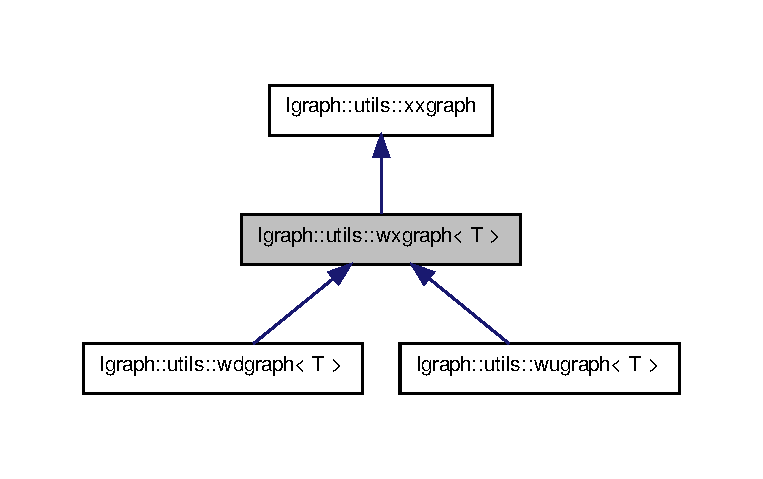
\includegraphics[width=350pt]{classlgraph_1_1utils_1_1wxgraph__inherit__graph}
\end{center}
\end{figure}


Collaboration diagram for lgraph\+:\+:utils\+:\+:wxgraph$<$ T $>$\+:\nopagebreak
\begin{figure}[H]
\begin{center}
\leavevmode
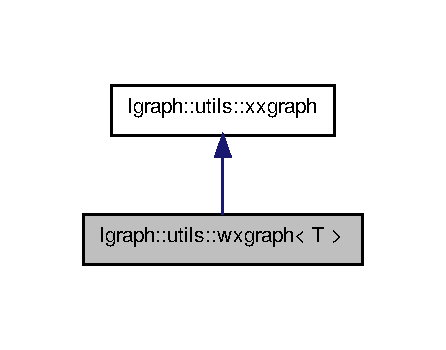
\includegraphics[width=214pt]{classlgraph_1_1utils_1_1wxgraph__coll__graph}
\end{center}
\end{figure}
\subsection*{Public Member Functions}
\begin{DoxyCompactItemize}
\item 
\hyperlink{classlgraph_1_1utils_1_1wxgraph_aaf4bc23e2bc74fd2a28aff2f56c6dbb2}{wxgraph} ()\hypertarget{classlgraph_1_1utils_1_1wxgraph_aaf4bc23e2bc74fd2a28aff2f56c6dbb2}{}\label{classlgraph_1_1utils_1_1wxgraph_aaf4bc23e2bc74fd2a28aff2f56c6dbb2}

\begin{DoxyCompactList}\small\item\em Constructor. \end{DoxyCompactList}\item 
virtual \hyperlink{classlgraph_1_1utils_1_1wxgraph_a970197826a0b64152fd812929b9038f1}{$\sim$wxgraph} ()\hypertarget{classlgraph_1_1utils_1_1wxgraph_a970197826a0b64152fd812929b9038f1}{}\label{classlgraph_1_1utils_1_1wxgraph_a970197826a0b64152fd812929b9038f1}

\begin{DoxyCompactList}\small\item\em Destructor. \end{DoxyCompactList}\item 
void \hyperlink{classlgraph_1_1utils_1_1wxgraph_a566ae9fe69209230ef159ed350ab8f7f}{init} (size\+\_\+t n)
\begin{DoxyCompactList}\small\item\em Initialises the attributes of a graph with {\itshape n} nodes. \end{DoxyCompactList}\item 
\hyperlink{classlgraph_1_1utils_1_1wxgraph}{wxgraph} \& \hyperlink{classlgraph_1_1utils_1_1wxgraph_a09fdb762864b9c663f8e2acf835e5191}{operator=} (const \hyperlink{classlgraph_1_1utils_1_1wxgraph}{wxgraph} \&g)
\begin{DoxyCompactList}\small\item\em Assignation operator for undirected weighted graphs. \end{DoxyCompactList}\item 
virtual void \hyperlink{classlgraph_1_1utils_1_1wxgraph_a8bee4a49537954adf70d720e0677caee}{add\+\_\+edge} (const \hyperlink{namespacelgraph_1_1utils_a6510284ce1b1ae5dc97ce5d2de426e10}{edge} \&e, const T \&w)=0
\begin{DoxyCompactList}\small\item\em Adds an edge to this graph. \end{DoxyCompactList}\item 
void \hyperlink{classlgraph_1_1utils_1_1wxgraph_a972a2483966f4b1d485c5d14157ee9be}{add\+\_\+edges} (const vector$<$ \hyperlink{namespacelgraph_1_1utils_a6510284ce1b1ae5dc97ce5d2de426e10}{edge} $>$ \&edge\+\_\+list, const vector$<$ T $>$ \&ws)
\begin{DoxyCompactList}\small\item\em Adds all edges taken from a list. \end{DoxyCompactList}\item 
virtual void \hyperlink{classlgraph_1_1utils_1_1wxgraph_a2cc33d25e8e593fa48cc05fdf0e96f9f}{add\+\_\+edge} (\hyperlink{namespacelgraph_1_1utils_a7bd66ede3805ef121bc2835bd48de0cf}{node} u, \hyperlink{namespacelgraph_1_1utils_a7bd66ede3805ef121bc2835bd48de0cf}{node} v, const T \&w)=0
\begin{DoxyCompactList}\small\item\em Adds an edge between nodes {\itshape u} and {\itshape v}. \end{DoxyCompactList}\item 
virtual void \hyperlink{classlgraph_1_1utils_1_1wxgraph_a5149c486108dfa06ee99c5ac09e46700}{remove\+\_\+edge} (const \hyperlink{namespacelgraph_1_1utils_a6510284ce1b1ae5dc97ce5d2de426e10}{edge} \&e)=0
\begin{DoxyCompactList}\small\item\em Removes an edge from this graph. \end{DoxyCompactList}\item 
void \hyperlink{classlgraph_1_1utils_1_1wxgraph_a4188b82f50e962b28c2c076b7978a854}{remove\+\_\+edges} (const vector$<$ \hyperlink{namespacelgraph_1_1utils_a6510284ce1b1ae5dc97ce5d2de426e10}{edge} $>$ \&edge\+\_\+list)
\begin{DoxyCompactList}\small\item\em Removes all edges taken from a list. \end{DoxyCompactList}\item 
virtual void \hyperlink{classlgraph_1_1utils_1_1wxgraph_aa5bf6c53cc0097621e7df44c32a0e2fc}{remove\+\_\+edge} (\hyperlink{namespacelgraph_1_1utils_a7bd66ede3805ef121bc2835bd48de0cf}{node} u, \hyperlink{namespacelgraph_1_1utils_a7bd66ede3805ef121bc2835bd48de0cf}{node} v)=0
\begin{DoxyCompactList}\small\item\em Removes an edge from this graph. \end{DoxyCompactList}\item 
void \hyperlink{classlgraph_1_1utils_1_1wxgraph_a421bc8166e35335445e45efc680ebe3f}{clear} ()
\begin{DoxyCompactList}\small\item\em Deletes all memory used by the graph. \end{DoxyCompactList}\item 
bool \hyperlink{classlgraph_1_1utils_1_1wxgraph_adda596cfbf72080d46ab445679fe092f}{is\+\_\+weighted} () const \hypertarget{classlgraph_1_1utils_1_1wxgraph_adda596cfbf72080d46ab445679fe092f}{}\label{classlgraph_1_1utils_1_1wxgraph_adda596cfbf72080d46ab445679fe092f}

\begin{DoxyCompactList}\small\item\em Returns whether this graph is weighted or not (returns true). \end{DoxyCompactList}\item 
virtual T \hyperlink{classlgraph_1_1utils_1_1wxgraph_ae634779d8d7f973fb7b7d2d9fb33c5c2}{edge\+\_\+weight} (\hyperlink{namespacelgraph_1_1utils_a7bd66ede3805ef121bc2835bd48de0cf}{node} u, \hyperlink{namespacelgraph_1_1utils_a7bd66ede3805ef121bc2835bd48de0cf}{node} v) const =0
\begin{DoxyCompactList}\small\item\em Returns the weight of the edge ({\itshape u}, {\itshape v}) \end{DoxyCompactList}\item 
const \hyperlink{namespacelgraph_1_1utils_a11e7963f3637ea13778b8d3e69d2c17f}{weight\+\_\+list}$<$ T $>$ \& \hyperlink{classlgraph_1_1utils_1_1wxgraph_a06252e99191d39329947c3a5eef43e73}{get\+\_\+weights} (\hyperlink{namespacelgraph_1_1utils_a7bd66ede3805ef121bc2835bd48de0cf}{node} u) const 
\begin{DoxyCompactList}\small\item\em Returns a constant reference to all the weights of node {\itshape u}. \end{DoxyCompactList}\item 
void \hyperlink{classlgraph_1_1utils_1_1wxgraph_a23c629eb031e31681749da793f933548}{get\+\_\+weights} (\hyperlink{namespacelgraph_1_1utils_a7bd66ede3805ef121bc2835bd48de0cf}{node} u, \hyperlink{namespacelgraph_1_1utils_a11e7963f3637ea13778b8d3e69d2c17f}{weight\+\_\+list}$<$ T $>$ \&ws) const 
\begin{DoxyCompactList}\small\item\em Returns the weights to all neighbours of node {\itshape u}. \end{DoxyCompactList}\item 
void \hyperlink{classlgraph_1_1utils_1_1wxgraph_a73b6c8887d5088750ee2cc98c45089c6}{edges} (vector$<$ pair$<$ \hyperlink{namespacelgraph_1_1utils_a6510284ce1b1ae5dc97ce5d2de426e10}{edge}, T $>$ $>$ \&all\+\_\+edges) const 
\begin{DoxyCompactList}\small\item\em Returns all unique edges of this graph. \end{DoxyCompactList}\item 
void \hyperlink{classlgraph_1_1utils_1_1wxgraph_a6c58b1f9bd596b3a12c181119eee9da2}{edges} (vector$<$ \hyperlink{namespacelgraph_1_1utils_a6510284ce1b1ae5dc97ce5d2de426e10}{edge} $>$ \&all\+\_\+edges) const 
\begin{DoxyCompactList}\small\item\em Returns all unique edges of this graph without their weights. \end{DoxyCompactList}\item 
virtual \hyperlink{classlgraph_1_1utils_1_1uxgraph}{uxgraph} $\ast$ \hyperlink{classlgraph_1_1utils_1_1wxgraph_a66d7a1fb48324c361d59dfa2d13db9eb}{to\+\_\+unweighted} () const =0
\begin{DoxyCompactList}\small\item\em Converts this graph into an unweighted graph. \end{DoxyCompactList}\item 
bool \hyperlink{classlgraph_1_1utils_1_1wxgraph_a329e674f9e3543f3347343470d82d404}{read\+\_\+from\+\_\+file} (const string \&filename)\hypertarget{classlgraph_1_1utils_1_1wxgraph_a329e674f9e3543f3347343470d82d404}{}\label{classlgraph_1_1utils_1_1wxgraph_a329e674f9e3543f3347343470d82d404}

\begin{DoxyCompactList}\small\item\em Reads the graph from a file. \end{DoxyCompactList}\item 
bool \hyperlink{classlgraph_1_1utils_1_1wxgraph_a74bb3ab0064749a8062c33a9213a233f}{read\+\_\+from\+\_\+file} (const char $\ast$filename)\hypertarget{classlgraph_1_1utils_1_1wxgraph_a74bb3ab0064749a8062c33a9213a233f}{}\label{classlgraph_1_1utils_1_1wxgraph_a74bb3ab0064749a8062c33a9213a233f}

\begin{DoxyCompactList}\small\item\em Reads the graph from a file. \end{DoxyCompactList}\item 
bool \hyperlink{classlgraph_1_1utils_1_1wxgraph_aff18a1cb62b8580956e8ddbb042e65e9}{store\+\_\+in\+\_\+file} (const string \&filename)\hypertarget{classlgraph_1_1utils_1_1wxgraph_aff18a1cb62b8580956e8ddbb042e65e9}{}\label{classlgraph_1_1utils_1_1wxgraph_aff18a1cb62b8580956e8ddbb042e65e9}

\begin{DoxyCompactList}\small\item\em Stores the graph in a file. \end{DoxyCompactList}\item 
bool \hyperlink{classlgraph_1_1utils_1_1wxgraph_aaa403d0b1dbca1e8e6d9cb30260e26df}{store\+\_\+in\+\_\+file} (const char $\ast$filename)\hypertarget{classlgraph_1_1utils_1_1wxgraph_aaa403d0b1dbca1e8e6d9cb30260e26df}{}\label{classlgraph_1_1utils_1_1wxgraph_aaa403d0b1dbca1e8e6d9cb30260e26df}

\begin{DoxyCompactList}\small\item\em Stores the graph in a file. \end{DoxyCompactList}\item 
size\+\_\+t \hyperlink{classlgraph_1_1utils_1_1xxgraph_af41baf2c098e872731ad646aeec1b382}{add\+\_\+node} ()
\begin{DoxyCompactList}\small\item\em Adds one node to the graph. \end{DoxyCompactList}\item 
size\+\_\+t \hyperlink{classlgraph_1_1utils_1_1xxgraph_af4f3782c1a55f73c6f34f2f2c26fb404}{add\+\_\+n\+\_\+nodes} (\hyperlink{namespacelgraph_1_1utils_a7bd66ede3805ef121bc2835bd48de0cf}{node} n)
\begin{DoxyCompactList}\small\item\em Adds {\itshape n} nodes to the graph. \end{DoxyCompactList}\item 
bool \hyperlink{classlgraph_1_1utils_1_1xxgraph_a026ab064c2be26790cc1f547be2157c9}{has\+\_\+node} (\hyperlink{namespacelgraph_1_1utils_a7bd66ede3805ef121bc2835bd48de0cf}{node} u) const \hypertarget{classlgraph_1_1utils_1_1xxgraph_a026ab064c2be26790cc1f547be2157c9}{}\label{classlgraph_1_1utils_1_1xxgraph_a026ab064c2be26790cc1f547be2157c9}

\begin{DoxyCompactList}\small\item\em Returns true if node {\itshape u} is in this graph. \end{DoxyCompactList}\item 
virtual bool \hyperlink{classlgraph_1_1utils_1_1xxgraph_a9e94100afc70b09049432f196550407c}{has\+\_\+edge} (\hyperlink{namespacelgraph_1_1utils_a7bd66ede3805ef121bc2835bd48de0cf}{node} u, \hyperlink{namespacelgraph_1_1utils_a7bd66ede3805ef121bc2835bd48de0cf}{node} v) const =0
\begin{DoxyCompactList}\small\item\em Returns true if there is an edge between nodes {\itshape u} and {\itshape v}. \end{DoxyCompactList}\item 
size\+\_\+t \hyperlink{classlgraph_1_1utils_1_1xxgraph_ad345f1fbf1dee34e1579b5aea9aef9b2}{n\+\_\+nodes} () const 
\begin{DoxyCompactList}\small\item\em Returns the number of nodes. \end{DoxyCompactList}\item 
size\+\_\+t \hyperlink{classlgraph_1_1utils_1_1xxgraph_af3f7c3835406c2cbf70479ae1c0253c9}{n\+\_\+edges} () const 
\begin{DoxyCompactList}\small\item\em Returns the number of edges. \end{DoxyCompactList}\item 
void \hyperlink{classlgraph_1_1utils_1_1xxgraph_a99f83387aa9f59b861e675251be5a3ad}{nodes} (vector$<$ \hyperlink{namespacelgraph_1_1utils_a7bd66ede3805ef121bc2835bd48de0cf}{node} $>$ \&all\+\_\+nodes) const \hypertarget{classlgraph_1_1utils_1_1xxgraph_a99f83387aa9f59b861e675251be5a3ad}{}\label{classlgraph_1_1utils_1_1xxgraph_a99f83387aa9f59b861e675251be5a3ad}

\begin{DoxyCompactList}\small\item\em Returns all nodes (as integers) \end{DoxyCompactList}\item 
const \hyperlink{namespacelgraph_1_1utils_a0f2ef47028a466d26841709e705390ac}{neighbourhood} \& \hyperlink{classlgraph_1_1utils_1_1xxgraph_a2c5332c4663c2d52828893f095a68202}{get\+\_\+neighbours} (\hyperlink{namespacelgraph_1_1utils_a7bd66ede3805ef121bc2835bd48de0cf}{node} u) const 
\begin{DoxyCompactList}\small\item\em Returns the neighbourhood of node u. \end{DoxyCompactList}\item 
size\+\_\+t \hyperlink{classlgraph_1_1utils_1_1xxgraph_af588aa4c68004a31aa143024cdb6dcc9}{degree} (\hyperlink{namespacelgraph_1_1utils_a7bd66ede3805ef121bc2835bd48de0cf}{node} u) const 
\begin{DoxyCompactList}\small\item\em Returns the number of neighbours of u. \end{DoxyCompactList}\item 
virtual bool \hyperlink{classlgraph_1_1utils_1_1xxgraph_a154376b6e55c4654622eb17ce738b5bb}{is\+\_\+directed} () const =0
\begin{DoxyCompactList}\small\item\em Returns whether the graph is directed or undirected. \end{DoxyCompactList}\item 
void \hyperlink{classlgraph_1_1utils_1_1xxgraph_a401454762f6b4b69f13ab0a10729c457}{get\+\_\+adjacency\+\_\+matrix} (vector$<$ vector$<$ bool $>$ $>$ \&adj\+\_\+mat) const \hypertarget{classlgraph_1_1utils_1_1xxgraph_a401454762f6b4b69f13ab0a10729c457}{}\label{classlgraph_1_1utils_1_1xxgraph_a401454762f6b4b69f13ab0a10729c457}

\begin{DoxyCompactList}\small\item\em Returns the adjacency matrix of this graph. \end{DoxyCompactList}\item 
void \hyperlink{classlgraph_1_1utils_1_1xxgraph_aff73f5ac4cd2732caa0c528eb1c1833c}{get\+\_\+degree\+\_\+sequence} (map$<$ size\+\_\+t, size\+\_\+t $>$ \&ds) const 
\begin{DoxyCompactList}\small\item\em Returns the degree sequence of the graph. \end{DoxyCompactList}\item 
size\+\_\+t \hyperlink{classlgraph_1_1utils_1_1xxgraph_ad4f25a8b29c6f26bc1567cb9c5a564ba}{n\+\_\+triangles} () const 
\begin{DoxyCompactList}\small\item\em Returns the number of triangles in this graph. \end{DoxyCompactList}\end{DoxyCompactItemize}
\subsection*{Protected Member Functions}
\begin{DoxyCompactItemize}
\item 
void \hyperlink{classlgraph_1_1utils_1_1wxgraph_a0b0c0b54acbc7816eb5b9958e61805cf}{initialise\+\_\+weights} (size\+\_\+t n)\hypertarget{classlgraph_1_1utils_1_1wxgraph_a0b0c0b54acbc7816eb5b9958e61805cf}{}\label{classlgraph_1_1utils_1_1wxgraph_a0b0c0b54acbc7816eb5b9958e61805cf}

\begin{DoxyCompactList}\small\item\em Initialises the list of weights. \end{DoxyCompactList}\item 
void \hyperlink{classlgraph_1_1utils_1_1wxgraph_a145f81ae3609af5ec038ace8b4413fad}{clear\+\_\+weights} ()\hypertarget{classlgraph_1_1utils_1_1wxgraph_a145f81ae3609af5ec038ace8b4413fad}{}\label{classlgraph_1_1utils_1_1wxgraph_a145f81ae3609af5ec038ace8b4413fad}

\begin{DoxyCompactList}\small\item\em Clears the list of weights. \end{DoxyCompactList}\item 
virtual void \hyperlink{classlgraph_1_1utils_1_1wxgraph_a2cf8037faaa1a2fd081e3d58e55a1932}{get\+\_\+unique\+\_\+edges} (vector$<$ pair$<$ \hyperlink{namespacelgraph_1_1utils_a6510284ce1b1ae5dc97ce5d2de426e10}{edge}, T $>$ $>$ \&\hyperlink{classlgraph_1_1utils_1_1wxgraph_a73b6c8887d5088750ee2cc98c45089c6}{edges}) const =0
\begin{DoxyCompactList}\small\item\em Computes the list of unique weighted edges of this graph. \end{DoxyCompactList}\item 
virtual void \hyperlink{classlgraph_1_1utils_1_1wxgraph_aaafce72400fb01e86b6c9f85a17406d0}{get\+\_\+unique\+\_\+edges} (vector$<$ \hyperlink{namespacelgraph_1_1utils_a6510284ce1b1ae5dc97ce5d2de426e10}{edge} $>$ \&\hyperlink{classlgraph_1_1utils_1_1wxgraph_a73b6c8887d5088750ee2cc98c45089c6}{edges}) const =0
\begin{DoxyCompactList}\small\item\em Computes the list of unique unweighted edges of this graph. \end{DoxyCompactList}\item 
size\+\_\+t \hyperlink{classlgraph_1_1utils_1_1xxgraph_aac7ef2134cad9529869f1334de7892d9}{get\+\_\+neighbour\+\_\+position} (const \hyperlink{namespacelgraph_1_1utils_a0f2ef47028a466d26841709e705390ac}{neighbourhood} \&n, \hyperlink{namespacelgraph_1_1utils_a7bd66ede3805ef121bc2835bd48de0cf}{node} u) const 
\begin{DoxyCompactList}\small\item\em Returns the position of node {\itshape u\textquotesingle{}s} position in the neighbourhood {\itshape n}. \end{DoxyCompactList}\item 
void \hyperlink{classlgraph_1_1utils_1_1xxgraph_a2201aaff5e9ffa29a9b3abfde705dd46}{initialise\+\_\+adjacency\+\_\+list} (size\+\_\+t n)\hypertarget{classlgraph_1_1utils_1_1xxgraph_a2201aaff5e9ffa29a9b3abfde705dd46}{}\label{classlgraph_1_1utils_1_1xxgraph_a2201aaff5e9ffa29a9b3abfde705dd46}

\begin{DoxyCompactList}\small\item\em Initialise the list of neighbourhoods with {\itshape n} instances. \end{DoxyCompactList}\item 
void \hyperlink{classlgraph_1_1utils_1_1xxgraph_a6523402d0ec66918b95de23d2bee38fc}{clear\+\_\+adjacency\+\_\+list} ()\hypertarget{classlgraph_1_1utils_1_1xxgraph_a6523402d0ec66918b95de23d2bee38fc}{}\label{classlgraph_1_1utils_1_1xxgraph_a6523402d0ec66918b95de23d2bee38fc}

\begin{DoxyCompactList}\small\item\em Clear the list of neighbourhoods. \end{DoxyCompactList}\item 
void \hyperlink{classlgraph_1_1utils_1_1xxgraph_abd983125be7f2f2b9c812326a4a39e6d}{initialise\+\_\+parent\+\_\+graph} (size\+\_\+t n)
\begin{DoxyCompactList}\small\item\em Initialises the adjacency list of this graph. \end{DoxyCompactList}\item 
void \hyperlink{classlgraph_1_1utils_1_1xxgraph_a8d213a8dfe716d344dd51d1bd37c0e2c}{clear\+\_\+parent\+\_\+graph} ()
\begin{DoxyCompactList}\small\item\em Clears the adjacency list of this graph. \end{DoxyCompactList}\end{DoxyCompactItemize}
\subsection*{Protected Attributes}
\begin{DoxyCompactItemize}
\item 
vector$<$ \hyperlink{namespacelgraph_1_1utils_a11e7963f3637ea13778b8d3e69d2c17f}{weight\+\_\+list}$<$ T $>$ $>$ \hyperlink{classlgraph_1_1utils_1_1wxgraph_a15569c8c0fccb641709dc81eb0e29c94}{weights}
\begin{DoxyCompactList}\small\item\em Weight list for each node. \end{DoxyCompactList}\item 
vector$<$ \hyperlink{namespacelgraph_1_1utils_a0f2ef47028a466d26841709e705390ac}{neighbourhood} $>$ \hyperlink{classlgraph_1_1utils_1_1xxgraph_a1d5fda0d5aa89340f997428b982f966f}{adjacency\+\_\+list}\hypertarget{classlgraph_1_1utils_1_1xxgraph_a1d5fda0d5aa89340f997428b982f966f}{}\label{classlgraph_1_1utils_1_1xxgraph_a1d5fda0d5aa89340f997428b982f966f}

\begin{DoxyCompactList}\small\item\em The neighbourhood of every node. \end{DoxyCompactList}\item 
size\+\_\+t \hyperlink{classlgraph_1_1utils_1_1xxgraph_a217ebb1cd8946fedfbf94a9b22f7da48}{num\+\_\+edges}\hypertarget{classlgraph_1_1utils_1_1xxgraph_a217ebb1cd8946fedfbf94a9b22f7da48}{}\label{classlgraph_1_1utils_1_1xxgraph_a217ebb1cd8946fedfbf94a9b22f7da48}

\begin{DoxyCompactList}\small\item\em The amount of edges in this graph. \end{DoxyCompactList}\end{DoxyCompactItemize}
\subsection*{Friends}
\begin{DoxyCompactItemize}
\item 
ostream \& \hyperlink{classlgraph_1_1utils_1_1wxgraph_acd581d8cf39c384e6476c3fe2d419e3e}{operator$<$$<$} (ostream \&os, const \hyperlink{classlgraph_1_1utils_1_1wxgraph}{wxgraph}$<$ T $>$ \&g)
\begin{DoxyCompactList}\small\item\em Outputs to the ostream {\itshape os} this graph. \end{DoxyCompactList}\end{DoxyCompactItemize}


\subsection{Detailed Description}
\subsubsection*{template$<$class T$>$\\*
class lgraph\+::utils\+::wxgraph$<$ T $>$}

Abstract class for weighted (ux) graphs. 

This class implements the weighted graph data structure based on adjacency lists.


\begin{DoxyParams}{Parameters}
{\em T} & Parameter that indicates the type of the edge weights \\
\hline
\end{DoxyParams}


\subsection{Member Function Documentation}
\index{lgraph\+::utils\+::wxgraph@{lgraph\+::utils\+::wxgraph}!add\+\_\+edge@{add\+\_\+edge}}
\index{add\+\_\+edge@{add\+\_\+edge}!lgraph\+::utils\+::wxgraph@{lgraph\+::utils\+::wxgraph}}
\subsubsection[{\texorpdfstring{add\+\_\+edge(const edge \&e, const T \&w)=0}{add_edge(const edge &e, const T &w)=0}}]{\setlength{\rightskip}{0pt plus 5cm}template$<$class T$>$ virtual void {\bf lgraph\+::utils\+::wxgraph}$<$ T $>$\+::add\+\_\+edge (
\begin{DoxyParamCaption}
\item[{const {\bf edge} \&}]{e, }
\item[{const T \&}]{w}
\end{DoxyParamCaption}
)\hspace{0.3cm}{\ttfamily [pure virtual]}}\hypertarget{classlgraph_1_1utils_1_1wxgraph_a8bee4a49537954adf70d720e0677caee}{}\label{classlgraph_1_1utils_1_1wxgraph_a8bee4a49537954adf70d720e0677caee}


Adds an edge to this graph. 

The attribute \hyperlink{classlgraph_1_1utils_1_1xxgraph_a217ebb1cd8946fedfbf94a9b22f7da48}{num\+\_\+edges} is incremented by one. 
\begin{DoxyParams}{Parameters}
{\em e} & A pair of nodes \\
\hline
{\em w} & The weight of the edge \\
\hline
\end{DoxyParams}


Implemented in \hyperlink{classlgraph_1_1utils_1_1wugraph_a8e4db27ca594bc78cde948a7c9fa1f00}{lgraph\+::utils\+::wugraph$<$ T $>$}, and \hyperlink{classlgraph_1_1utils_1_1wdgraph_a28926dd95b2d19ee32adf5d5434af89b}{lgraph\+::utils\+::wdgraph$<$ T $>$}.

\index{lgraph\+::utils\+::wxgraph@{lgraph\+::utils\+::wxgraph}!add\+\_\+edge@{add\+\_\+edge}}
\index{add\+\_\+edge@{add\+\_\+edge}!lgraph\+::utils\+::wxgraph@{lgraph\+::utils\+::wxgraph}}
\subsubsection[{\texorpdfstring{add\+\_\+edge(node u, node v, const T \&w)=0}{add_edge(node u, node v, const T &w)=0}}]{\setlength{\rightskip}{0pt plus 5cm}template$<$class T$>$ virtual void {\bf lgraph\+::utils\+::wxgraph}$<$ T $>$\+::add\+\_\+edge (
\begin{DoxyParamCaption}
\item[{{\bf node}}]{u, }
\item[{{\bf node}}]{v, }
\item[{const T \&}]{w}
\end{DoxyParamCaption}
)\hspace{0.3cm}{\ttfamily [pure virtual]}}\hypertarget{classlgraph_1_1utils_1_1wxgraph_a2cc33d25e8e593fa48cc05fdf0e96f9f}{}\label{classlgraph_1_1utils_1_1wxgraph_a2cc33d25e8e593fa48cc05fdf0e96f9f}


Adds an edge between nodes {\itshape u} and {\itshape v}. 

The attribute \hyperlink{classlgraph_1_1utils_1_1xxgraph_a217ebb1cd8946fedfbf94a9b22f7da48}{num\+\_\+edges} is incremented by one.


\begin{DoxyParams}{Parameters}
{\em u} & The fist node of the edge \\
\hline
{\em v} & The second node of the edge \\
\hline
{\em w} & The weight of the edge \\
\hline
\end{DoxyParams}


Implemented in \hyperlink{classlgraph_1_1utils_1_1wugraph_a64d5de79fb869156ba3a110a68d6ea3f}{lgraph\+::utils\+::wugraph$<$ T $>$}, and \hyperlink{classlgraph_1_1utils_1_1wdgraph_a5c96c31a8b5d70829bf023382d7c1997}{lgraph\+::utils\+::wdgraph$<$ T $>$}.

\index{lgraph\+::utils\+::wxgraph@{lgraph\+::utils\+::wxgraph}!add\+\_\+edges@{add\+\_\+edges}}
\index{add\+\_\+edges@{add\+\_\+edges}!lgraph\+::utils\+::wxgraph@{lgraph\+::utils\+::wxgraph}}
\subsubsection[{\texorpdfstring{add\+\_\+edges(const vector$<$ edge $>$ \&edge\+\_\+list, const vector$<$ T $>$ \&ws)}{add_edges(const vector< edge > &edge_list, const vector< T > &ws)}}]{\setlength{\rightskip}{0pt plus 5cm}template$<$class T $>$ void {\bf lgraph\+::utils\+::wxgraph}$<$ T $>$\+::add\+\_\+edges (
\begin{DoxyParamCaption}
\item[{const vector$<$ {\bf edge} $>$ \&}]{edge\+\_\+list, }
\item[{const vector$<$ T $>$ \&}]{ws}
\end{DoxyParamCaption}
)}\hypertarget{classlgraph_1_1utils_1_1wxgraph_a972a2483966f4b1d485c5d14157ee9be}{}\label{classlgraph_1_1utils_1_1wxgraph_a972a2483966f4b1d485c5d14157ee9be}


Adds all edges taken from a list. 

The attribute \hyperlink{classlgraph_1_1utils_1_1xxgraph_a217ebb1cd8946fedfbf94a9b22f7da48}{num\+\_\+edges} is incremented as many times as elements there are in {\itshape edge\+\_\+list}. 
\begin{DoxyParams}{Parameters}
{\em edge\+\_\+list} & A list of pairs of nodes \\
\hline
{\em ws} & A list of weights. The i-\/th edge has weight {\itshape ws}\mbox{[}i\mbox{]}. \\
\hline
\end{DoxyParams}
\index{lgraph\+::utils\+::wxgraph@{lgraph\+::utils\+::wxgraph}!add\+\_\+n\+\_\+nodes@{add\+\_\+n\+\_\+nodes}}
\index{add\+\_\+n\+\_\+nodes@{add\+\_\+n\+\_\+nodes}!lgraph\+::utils\+::wxgraph@{lgraph\+::utils\+::wxgraph}}
\subsubsection[{\texorpdfstring{add\+\_\+n\+\_\+nodes(node n)}{add_n_nodes(node n)}}]{\setlength{\rightskip}{0pt plus 5cm}size\+\_\+t lgraph\+::utils\+::xxgraph\+::add\+\_\+n\+\_\+nodes (
\begin{DoxyParamCaption}
\item[{{\bf node}}]{n}
\end{DoxyParamCaption}
)\hspace{0.3cm}{\ttfamily [inherited]}}\hypertarget{classlgraph_1_1utils_1_1xxgraph_af4f3782c1a55f73c6f34f2f2c26fb404}{}\label{classlgraph_1_1utils_1_1xxgraph_af4f3782c1a55f73c6f34f2f2c26fb404}


Adds {\itshape n} nodes to the graph. 

The nodes are assigned consecutive, increasing values. \begin{DoxyReturn}{Returns}
Returns the index of the last node. 
\end{DoxyReturn}
\index{lgraph\+::utils\+::wxgraph@{lgraph\+::utils\+::wxgraph}!add\+\_\+node@{add\+\_\+node}}
\index{add\+\_\+node@{add\+\_\+node}!lgraph\+::utils\+::wxgraph@{lgraph\+::utils\+::wxgraph}}
\subsubsection[{\texorpdfstring{add\+\_\+node()}{add_node()}}]{\setlength{\rightskip}{0pt plus 5cm}size\+\_\+t lgraph\+::utils\+::xxgraph\+::add\+\_\+node (
\begin{DoxyParamCaption}
{}
\end{DoxyParamCaption}
)\hspace{0.3cm}{\ttfamily [inherited]}}\hypertarget{classlgraph_1_1utils_1_1xxgraph_af41baf2c098e872731ad646aeec1b382}{}\label{classlgraph_1_1utils_1_1xxgraph_af41baf2c098e872731ad646aeec1b382}


Adds one node to the graph. 

\begin{DoxyReturn}{Returns}
Returns the index of the new node 
\end{DoxyReturn}
\index{lgraph\+::utils\+::wxgraph@{lgraph\+::utils\+::wxgraph}!clear@{clear}}
\index{clear@{clear}!lgraph\+::utils\+::wxgraph@{lgraph\+::utils\+::wxgraph}}
\subsubsection[{\texorpdfstring{clear()}{clear()}}]{\setlength{\rightskip}{0pt plus 5cm}template$<$class T $>$ void {\bf lgraph\+::utils\+::wxgraph}$<$ T $>$\+::clear (
\begin{DoxyParamCaption}
{}
\end{DoxyParamCaption}
)}\hypertarget{classlgraph_1_1utils_1_1wxgraph_a421bc8166e35335445e45efc680ebe3f}{}\label{classlgraph_1_1utils_1_1wxgraph_a421bc8166e35335445e45efc680ebe3f}


Deletes all memory used by the graph. 

The value \hyperlink{classlgraph_1_1utils_1_1xxgraph_a217ebb1cd8946fedfbf94a9b22f7da48}{num\+\_\+edges} is set to 0. \index{lgraph\+::utils\+::wxgraph@{lgraph\+::utils\+::wxgraph}!clear\+\_\+parent\+\_\+graph@{clear\+\_\+parent\+\_\+graph}}
\index{clear\+\_\+parent\+\_\+graph@{clear\+\_\+parent\+\_\+graph}!lgraph\+::utils\+::wxgraph@{lgraph\+::utils\+::wxgraph}}
\subsubsection[{\texorpdfstring{clear\+\_\+parent\+\_\+graph()}{clear_parent_graph()}}]{\setlength{\rightskip}{0pt plus 5cm}void lgraph\+::utils\+::xxgraph\+::clear\+\_\+parent\+\_\+graph (
\begin{DoxyParamCaption}
{}
\end{DoxyParamCaption}
)\hspace{0.3cm}{\ttfamily [protected]}, {\ttfamily [inherited]}}\hypertarget{classlgraph_1_1utils_1_1xxgraph_a8d213a8dfe716d344dd51d1bd37c0e2c}{}\label{classlgraph_1_1utils_1_1xxgraph_a8d213a8dfe716d344dd51d1bd37c0e2c}


Clears the adjacency list of this graph. 

The value \hyperlink{classlgraph_1_1utils_1_1xxgraph_a217ebb1cd8946fedfbf94a9b22f7da48}{num\+\_\+edges} is set to 0. \index{lgraph\+::utils\+::wxgraph@{lgraph\+::utils\+::wxgraph}!degree@{degree}}
\index{degree@{degree}!lgraph\+::utils\+::wxgraph@{lgraph\+::utils\+::wxgraph}}
\subsubsection[{\texorpdfstring{degree(node u) const }{degree(node u) const }}]{\setlength{\rightskip}{0pt plus 5cm}size\+\_\+t lgraph\+::utils\+::xxgraph\+::degree (
\begin{DoxyParamCaption}
\item[{{\bf node}}]{u}
\end{DoxyParamCaption}
) const\hspace{0.3cm}{\ttfamily [inherited]}}\hypertarget{classlgraph_1_1utils_1_1xxgraph_af588aa4c68004a31aa143024cdb6dcc9}{}\label{classlgraph_1_1utils_1_1xxgraph_af588aa4c68004a31aa143024cdb6dcc9}


Returns the number of neighbours of u. 


\begin{DoxyParams}{Parameters}
{\em u} & The node whose neighbourhood size we want \\
\hline
\end{DoxyParams}
\begin{DoxyReturn}{Returns}
Returns the size of the neighbourhood of {\itshape u}, that is, the size of the list in \hyperlink{classlgraph_1_1utils_1_1xxgraph_a1d5fda0d5aa89340f997428b982f966f}{adjacency\+\_\+list}\mbox{[}u\mbox{]} 
\end{DoxyReturn}
\begin{DoxyPrecond}{Precondition}
{\itshape u} must be a node from the graph 
\end{DoxyPrecond}
\index{lgraph\+::utils\+::wxgraph@{lgraph\+::utils\+::wxgraph}!edge\+\_\+weight@{edge\+\_\+weight}}
\index{edge\+\_\+weight@{edge\+\_\+weight}!lgraph\+::utils\+::wxgraph@{lgraph\+::utils\+::wxgraph}}
\subsubsection[{\texorpdfstring{edge\+\_\+weight(node u, node v) const =0}{edge_weight(node u, node v) const =0}}]{\setlength{\rightskip}{0pt plus 5cm}template$<$class T$>$ virtual T {\bf lgraph\+::utils\+::wxgraph}$<$ T $>$\+::edge\+\_\+weight (
\begin{DoxyParamCaption}
\item[{{\bf node}}]{u, }
\item[{{\bf node}}]{v}
\end{DoxyParamCaption}
) const\hspace{0.3cm}{\ttfamily [pure virtual]}}\hypertarget{classlgraph_1_1utils_1_1wxgraph_ae634779d8d7f973fb7b7d2d9fb33c5c2}{}\label{classlgraph_1_1utils_1_1wxgraph_ae634779d8d7f973fb7b7d2d9fb33c5c2}


Returns the weight of the edge ({\itshape u}, {\itshape v}) 

\begin{DoxyPrecond}{Precondition}
The edge ({\itshape u}, {\itshape v}) must be in the graph 
\end{DoxyPrecond}


Implemented in \hyperlink{classlgraph_1_1utils_1_1wugraph_ace598c9cb108806a2a9a6ff4219377de}{lgraph\+::utils\+::wugraph$<$ T $>$}, and \hyperlink{classlgraph_1_1utils_1_1wdgraph_a1d86f87f61f47af9251945c14385c4e4}{lgraph\+::utils\+::wdgraph$<$ T $>$}.

\index{lgraph\+::utils\+::wxgraph@{lgraph\+::utils\+::wxgraph}!edges@{edges}}
\index{edges@{edges}!lgraph\+::utils\+::wxgraph@{lgraph\+::utils\+::wxgraph}}
\subsubsection[{\texorpdfstring{edges(vector$<$ pair$<$ edge, T $>$ $>$ \&all\+\_\+edges) const }{edges(vector< pair< edge, T > > &all_edges) const }}]{\setlength{\rightskip}{0pt plus 5cm}template$<$class T $>$ void {\bf lgraph\+::utils\+::wxgraph}$<$ T $>$\+::edges (
\begin{DoxyParamCaption}
\item[{vector$<$ pair$<$ {\bf edge}, T $>$ $>$ \&}]{all\+\_\+edges}
\end{DoxyParamCaption}
) const}\hypertarget{classlgraph_1_1utils_1_1wxgraph_a73b6c8887d5088750ee2cc98c45089c6}{}\label{classlgraph_1_1utils_1_1wxgraph_a73b6c8887d5088750ee2cc98c45089c6}


Returns all unique edges of this graph. 

See method \hyperlink{classlgraph_1_1utils_1_1wxgraph_a2cf8037faaa1a2fd081e3d58e55a1932}{get\+\_\+unique\+\_\+edges(vector$<$pair$<$edge,\+T$>$ $>$\& edges)const} for details. \index{lgraph\+::utils\+::wxgraph@{lgraph\+::utils\+::wxgraph}!edges@{edges}}
\index{edges@{edges}!lgraph\+::utils\+::wxgraph@{lgraph\+::utils\+::wxgraph}}
\subsubsection[{\texorpdfstring{edges(vector$<$ edge $>$ \&all\+\_\+edges) const }{edges(vector< edge > &all_edges) const }}]{\setlength{\rightskip}{0pt plus 5cm}template$<$class T $>$ void {\bf lgraph\+::utils\+::wxgraph}$<$ T $>$\+::edges (
\begin{DoxyParamCaption}
\item[{vector$<$ {\bf edge} $>$ \&}]{all\+\_\+edges}
\end{DoxyParamCaption}
) const}\hypertarget{classlgraph_1_1utils_1_1wxgraph_a6c58b1f9bd596b3a12c181119eee9da2}{}\label{classlgraph_1_1utils_1_1wxgraph_a6c58b1f9bd596b3a12c181119eee9da2}


Returns all unique edges of this graph without their weights. 

See method \hyperlink{classlgraph_1_1utils_1_1wxgraph_aaafce72400fb01e86b6c9f85a17406d0}{get\+\_\+unique\+\_\+edges(vector$<$edge$>$\& edges)const} for details. \index{lgraph\+::utils\+::wxgraph@{lgraph\+::utils\+::wxgraph}!get\+\_\+degree\+\_\+sequence@{get\+\_\+degree\+\_\+sequence}}
\index{get\+\_\+degree\+\_\+sequence@{get\+\_\+degree\+\_\+sequence}!lgraph\+::utils\+::wxgraph@{lgraph\+::utils\+::wxgraph}}
\subsubsection[{\texorpdfstring{get\+\_\+degree\+\_\+sequence(map$<$ size\+\_\+t, size\+\_\+t $>$ \&ds) const }{get_degree_sequence(map< size_t, size_t > &ds) const }}]{\setlength{\rightskip}{0pt plus 5cm}void lgraph\+::utils\+::xxgraph\+::get\+\_\+degree\+\_\+sequence (
\begin{DoxyParamCaption}
\item[{map$<$ size\+\_\+t, size\+\_\+t $>$ \&}]{ds}
\end{DoxyParamCaption}
) const\hspace{0.3cm}{\ttfamily [inherited]}}\hypertarget{classlgraph_1_1utils_1_1xxgraph_aff73f5ac4cd2732caa0c528eb1c1833c}{}\label{classlgraph_1_1utils_1_1xxgraph_aff73f5ac4cd2732caa0c528eb1c1833c}


Returns the degree sequence of the graph. 


\begin{DoxyParams}[1]{Parameters}
\mbox{\tt out}  & {\em ds} & A list of pairs\+: for each degree the amount of nodes in this graph that have that degree. The degree of a node is detailed in \hyperlink{classlgraph_1_1utils_1_1xxgraph_af588aa4c68004a31aa143024cdb6dcc9}{degree} \\
\hline
\end{DoxyParams}
\index{lgraph\+::utils\+::wxgraph@{lgraph\+::utils\+::wxgraph}!get\+\_\+neighbour\+\_\+position@{get\+\_\+neighbour\+\_\+position}}
\index{get\+\_\+neighbour\+\_\+position@{get\+\_\+neighbour\+\_\+position}!lgraph\+::utils\+::wxgraph@{lgraph\+::utils\+::wxgraph}}
\subsubsection[{\texorpdfstring{get\+\_\+neighbour\+\_\+position(const neighbourhood \&n, node u) const }{get_neighbour_position(const neighbourhood &n, node u) const }}]{\setlength{\rightskip}{0pt plus 5cm}size\+\_\+t lgraph\+::utils\+::xxgraph\+::get\+\_\+neighbour\+\_\+position (
\begin{DoxyParamCaption}
\item[{const {\bf neighbourhood} \&}]{n, }
\item[{{\bf node}}]{u}
\end{DoxyParamCaption}
) const\hspace{0.3cm}{\ttfamily [protected]}, {\ttfamily [inherited]}}\hypertarget{classlgraph_1_1utils_1_1xxgraph_aac7ef2134cad9529869f1334de7892d9}{}\label{classlgraph_1_1utils_1_1xxgraph_aac7ef2134cad9529869f1334de7892d9}


Returns the position of node {\itshape u\textquotesingle{}s} position in the neighbourhood {\itshape n}. 

If the position is equal to the number of elements of the list {\itshape n} then {\itshape u} is in the list. Performs a linear search to find it. 
\begin{DoxyParams}{Parameters}
{\em n} & The neighbourhood of a node in the graph \\
\hline
{\em u} & The node to look for in the neighbourhood \\
\hline
\end{DoxyParams}
\begin{DoxyReturn}{Returns}
Returns a value equal to the number of elements in the list {\itshape n} if node {\itshape u} is not in it. Returns a value smaller than that if otherwise. 
\end{DoxyReturn}
\index{lgraph\+::utils\+::wxgraph@{lgraph\+::utils\+::wxgraph}!get\+\_\+neighbours@{get\+\_\+neighbours}}
\index{get\+\_\+neighbours@{get\+\_\+neighbours}!lgraph\+::utils\+::wxgraph@{lgraph\+::utils\+::wxgraph}}
\subsubsection[{\texorpdfstring{get\+\_\+neighbours(node u) const }{get_neighbours(node u) const }}]{\setlength{\rightskip}{0pt plus 5cm}const {\bf neighbourhood} \& lgraph\+::utils\+::xxgraph\+::get\+\_\+neighbours (
\begin{DoxyParamCaption}
\item[{{\bf node}}]{u}
\end{DoxyParamCaption}
) const\hspace{0.3cm}{\ttfamily [inherited]}}\hypertarget{classlgraph_1_1utils_1_1xxgraph_a2c5332c4663c2d52828893f095a68202}{}\label{classlgraph_1_1utils_1_1xxgraph_a2c5332c4663c2d52828893f095a68202}


Returns the neighbourhood of node u. 


\begin{DoxyParams}{Parameters}
{\em u} & The node whose neighbourhood we want \\
\hline
\end{DoxyParams}
\begin{DoxyPrecond}{Precondition}
{\itshape u} must be a node from the graph 
\end{DoxyPrecond}
\index{lgraph\+::utils\+::wxgraph@{lgraph\+::utils\+::wxgraph}!get\+\_\+unique\+\_\+edges@{get\+\_\+unique\+\_\+edges}}
\index{get\+\_\+unique\+\_\+edges@{get\+\_\+unique\+\_\+edges}!lgraph\+::utils\+::wxgraph@{lgraph\+::utils\+::wxgraph}}
\subsubsection[{\texorpdfstring{get\+\_\+unique\+\_\+edges(vector$<$ pair$<$ edge, T $>$ $>$ \&edges) const =0}{get_unique_edges(vector< pair< edge, T > > &edges) const =0}}]{\setlength{\rightskip}{0pt plus 5cm}template$<$class T$>$ virtual void {\bf lgraph\+::utils\+::wxgraph}$<$ T $>$\+::get\+\_\+unique\+\_\+edges (
\begin{DoxyParamCaption}
\item[{vector$<$ pair$<$ {\bf edge}, T $>$ $>$ \&}]{edges}
\end{DoxyParamCaption}
) const\hspace{0.3cm}{\ttfamily [protected]}, {\ttfamily [pure virtual]}}\hypertarget{classlgraph_1_1utils_1_1wxgraph_a2cf8037faaa1a2fd081e3d58e55a1932}{}\label{classlgraph_1_1utils_1_1wxgraph_a2cf8037faaa1a2fd081e3d58e55a1932}


Computes the list of unique weighted edges of this graph. 

A weighted edge is a pair of an edge and a value representing the weight of that edge. An edge is a pair of indices, each of which is within the interval \mbox{[}0,{\itshape n}) where {\itshape n} is the number of nodes of this graph.


\begin{DoxyParams}[1]{Parameters}
\mbox{\tt out}  & {\em edges} & The collection of weighted edges \\
\hline
\end{DoxyParams}
\begin{DoxyReturn}{Returns}
Stores in \hyperlink{classlgraph_1_1utils_1_1wxgraph_a73b6c8887d5088750ee2cc98c45089c6}{edges} the list of weighted edges of this graph 
\end{DoxyReturn}


Implemented in \hyperlink{classlgraph_1_1utils_1_1wugraph_a603d54feaa555bcb9747eb2f48891447}{lgraph\+::utils\+::wugraph$<$ T $>$}, and \hyperlink{classlgraph_1_1utils_1_1wdgraph_a243f794a014b124483066d7cf1715c22}{lgraph\+::utils\+::wdgraph$<$ T $>$}.

\index{lgraph\+::utils\+::wxgraph@{lgraph\+::utils\+::wxgraph}!get\+\_\+unique\+\_\+edges@{get\+\_\+unique\+\_\+edges}}
\index{get\+\_\+unique\+\_\+edges@{get\+\_\+unique\+\_\+edges}!lgraph\+::utils\+::wxgraph@{lgraph\+::utils\+::wxgraph}}
\subsubsection[{\texorpdfstring{get\+\_\+unique\+\_\+edges(vector$<$ edge $>$ \&edges) const =0}{get_unique_edges(vector< edge > &edges) const =0}}]{\setlength{\rightskip}{0pt plus 5cm}template$<$class T$>$ virtual void {\bf lgraph\+::utils\+::wxgraph}$<$ T $>$\+::get\+\_\+unique\+\_\+edges (
\begin{DoxyParamCaption}
\item[{vector$<$ {\bf edge} $>$ \&}]{edges}
\end{DoxyParamCaption}
) const\hspace{0.3cm}{\ttfamily [protected]}, {\ttfamily [pure virtual]}}\hypertarget{classlgraph_1_1utils_1_1wxgraph_aaafce72400fb01e86b6c9f85a17406d0}{}\label{classlgraph_1_1utils_1_1wxgraph_aaafce72400fb01e86b6c9f85a17406d0}


Computes the list of unique unweighted edges of this graph. 

An unweighted edge is a pair of indices each of which is within the interval \mbox{[}0,{\itshape n}) where {\itshape n} is the number of nodes of this graph.


\begin{DoxyParams}[1]{Parameters}
\mbox{\tt out}  & {\em edges} & The collection of unweighted edges \\
\hline
\end{DoxyParams}
\begin{DoxyReturn}{Returns}
Stores in \hyperlink{classlgraph_1_1utils_1_1wxgraph_a73b6c8887d5088750ee2cc98c45089c6}{edges} the list of unweighted edges of this graph 
\end{DoxyReturn}


Implemented in \hyperlink{classlgraph_1_1utils_1_1wugraph_a943b9edf2c45d3cac296836c7fab052d}{lgraph\+::utils\+::wugraph$<$ T $>$}, and \hyperlink{classlgraph_1_1utils_1_1wdgraph_ae6ee2acf01c1e0e07ea8bdd0f951ec77}{lgraph\+::utils\+::wdgraph$<$ T $>$}.

\index{lgraph\+::utils\+::wxgraph@{lgraph\+::utils\+::wxgraph}!get\+\_\+weights@{get\+\_\+weights}}
\index{get\+\_\+weights@{get\+\_\+weights}!lgraph\+::utils\+::wxgraph@{lgraph\+::utils\+::wxgraph}}
\subsubsection[{\texorpdfstring{get\+\_\+weights(node u) const }{get_weights(node u) const }}]{\setlength{\rightskip}{0pt plus 5cm}template$<$class T $>$ const {\bf weight\+\_\+list}$<$ T $>$ \& {\bf lgraph\+::utils\+::wxgraph}$<$ T $>$\+::get\+\_\+weights (
\begin{DoxyParamCaption}
\item[{{\bf node}}]{u}
\end{DoxyParamCaption}
) const}\hypertarget{classlgraph_1_1utils_1_1wxgraph_a06252e99191d39329947c3a5eef43e73}{}\label{classlgraph_1_1utils_1_1wxgraph_a06252e99191d39329947c3a5eef43e73}


Returns a constant reference to all the weights of node {\itshape u}. 


\begin{DoxyParams}{Parameters}
{\em u} & The node whose weight list is requested \\
\hline
\end{DoxyParams}
\begin{DoxyReturn}{Returns}
The weight list of node {\itshape u} 
\end{DoxyReturn}
\index{lgraph\+::utils\+::wxgraph@{lgraph\+::utils\+::wxgraph}!get\+\_\+weights@{get\+\_\+weights}}
\index{get\+\_\+weights@{get\+\_\+weights}!lgraph\+::utils\+::wxgraph@{lgraph\+::utils\+::wxgraph}}
\subsubsection[{\texorpdfstring{get\+\_\+weights(node u, weight\+\_\+list$<$ T $>$ \&ws) const }{get_weights(node u, weight_list< T > &ws) const }}]{\setlength{\rightskip}{0pt plus 5cm}template$<$class T $>$ void {\bf lgraph\+::utils\+::wxgraph}$<$ T $>$\+::get\+\_\+weights (
\begin{DoxyParamCaption}
\item[{{\bf node}}]{u, }
\item[{{\bf weight\+\_\+list}$<$ T $>$ \&}]{ws}
\end{DoxyParamCaption}
) const}\hypertarget{classlgraph_1_1utils_1_1wxgraph_a23c629eb031e31681749da793f933548}{}\label{classlgraph_1_1utils_1_1wxgraph_a23c629eb031e31681749da793f933548}


Returns the weights to all neighbours of node {\itshape u}. 

\begin{DoxyPrecond}{Precondition}
{\itshape u} must be in the graph 
\end{DoxyPrecond}
\index{lgraph\+::utils\+::wxgraph@{lgraph\+::utils\+::wxgraph}!has\+\_\+edge@{has\+\_\+edge}}
\index{has\+\_\+edge@{has\+\_\+edge}!lgraph\+::utils\+::wxgraph@{lgraph\+::utils\+::wxgraph}}
\subsubsection[{\texorpdfstring{has\+\_\+edge(node u, node v) const =0}{has_edge(node u, node v) const =0}}]{\setlength{\rightskip}{0pt plus 5cm}virtual bool lgraph\+::utils\+::xxgraph\+::has\+\_\+edge (
\begin{DoxyParamCaption}
\item[{{\bf node}}]{u, }
\item[{{\bf node}}]{v}
\end{DoxyParamCaption}
) const\hspace{0.3cm}{\ttfamily [pure virtual]}, {\ttfamily [inherited]}}\hypertarget{classlgraph_1_1utils_1_1xxgraph_a9e94100afc70b09049432f196550407c}{}\label{classlgraph_1_1utils_1_1xxgraph_a9e94100afc70b09049432f196550407c}


Returns true if there is an edge between nodes {\itshape u} and {\itshape v}. 

\begin{DoxyPrecond}{Precondition}
{\itshape u} and {\itshape v} must be in the graph 
\end{DoxyPrecond}


Implemented in \hyperlink{classlgraph_1_1utils_1_1wugraph_a5d729aece87dbda408211b12ad4856d1}{lgraph\+::utils\+::wugraph$<$ T $>$}, \hyperlink{classlgraph_1_1utils_1_1wdgraph_ac74f172c5a6bdbf56ac5a4013fae880a}{lgraph\+::utils\+::wdgraph$<$ T $>$}, \hyperlink{classlgraph_1_1utils_1_1uugraph_a1970a2f371f20284478246a83292f9bb}{lgraph\+::utils\+::uugraph}, and \hyperlink{classlgraph_1_1utils_1_1udgraph_aebc98d234955028116978eff9c13445b}{lgraph\+::utils\+::udgraph}.

\index{lgraph\+::utils\+::wxgraph@{lgraph\+::utils\+::wxgraph}!init@{init}}
\index{init@{init}!lgraph\+::utils\+::wxgraph@{lgraph\+::utils\+::wxgraph}}
\subsubsection[{\texorpdfstring{init(size\+\_\+t n)}{init(size_t n)}}]{\setlength{\rightskip}{0pt plus 5cm}template$<$class T $>$ void {\bf lgraph\+::utils\+::wxgraph}$<$ T $>$\+::init (
\begin{DoxyParamCaption}
\item[{size\+\_\+t}]{n}
\end{DoxyParamCaption}
)\hspace{0.3cm}{\ttfamily [virtual]}}\hypertarget{classlgraph_1_1utils_1_1wxgraph_a566ae9fe69209230ef159ed350ab8f7f}{}\label{classlgraph_1_1utils_1_1wxgraph_a566ae9fe69209230ef159ed350ab8f7f}


Initialises the attributes of a graph with {\itshape n} nodes. 

First, it clears all the memory allocated so far. Then, initialises all the attributes so that it can store all the necessary information. 
\begin{DoxyParams}{Parameters}
{\em n} & Number of nodes of the graph \\
\hline
\end{DoxyParams}


Implements \hyperlink{classlgraph_1_1utils_1_1xxgraph_a2ac8b3e71fa0550248c692a19ea04d0d}{lgraph\+::utils\+::xxgraph}.

\index{lgraph\+::utils\+::wxgraph@{lgraph\+::utils\+::wxgraph}!initialise\+\_\+parent\+\_\+graph@{initialise\+\_\+parent\+\_\+graph}}
\index{initialise\+\_\+parent\+\_\+graph@{initialise\+\_\+parent\+\_\+graph}!lgraph\+::utils\+::wxgraph@{lgraph\+::utils\+::wxgraph}}
\subsubsection[{\texorpdfstring{initialise\+\_\+parent\+\_\+graph(size\+\_\+t n)}{initialise_parent_graph(size_t n)}}]{\setlength{\rightskip}{0pt plus 5cm}void lgraph\+::utils\+::xxgraph\+::initialise\+\_\+parent\+\_\+graph (
\begin{DoxyParamCaption}
\item[{size\+\_\+t}]{n}
\end{DoxyParamCaption}
)\hspace{0.3cm}{\ttfamily [protected]}, {\ttfamily [inherited]}}\hypertarget{classlgraph_1_1utils_1_1xxgraph_abd983125be7f2f2b9c812326a4a39e6d}{}\label{classlgraph_1_1utils_1_1xxgraph_abd983125be7f2f2b9c812326a4a39e6d}


Initialises the adjacency list of this graph. 

The value \hyperlink{classlgraph_1_1utils_1_1xxgraph_a217ebb1cd8946fedfbf94a9b22f7da48}{num\+\_\+edges} is set to 0. \index{lgraph\+::utils\+::wxgraph@{lgraph\+::utils\+::wxgraph}!is\+\_\+directed@{is\+\_\+directed}}
\index{is\+\_\+directed@{is\+\_\+directed}!lgraph\+::utils\+::wxgraph@{lgraph\+::utils\+::wxgraph}}
\subsubsection[{\texorpdfstring{is\+\_\+directed() const =0}{is_directed() const =0}}]{\setlength{\rightskip}{0pt plus 5cm}virtual bool lgraph\+::utils\+::xxgraph\+::is\+\_\+directed (
\begin{DoxyParamCaption}
{}
\end{DoxyParamCaption}
) const\hspace{0.3cm}{\ttfamily [pure virtual]}, {\ttfamily [inherited]}}\hypertarget{classlgraph_1_1utils_1_1xxgraph_a154376b6e55c4654622eb17ce738b5bb}{}\label{classlgraph_1_1utils_1_1xxgraph_a154376b6e55c4654622eb17ce738b5bb}


Returns whether the graph is directed or undirected. 

\begin{DoxyReturn}{Returns}
Returns true if the graph is directed. Returns false if otherwise. 
\end{DoxyReturn}


Implemented in \hyperlink{classlgraph_1_1utils_1_1wugraph_a3ed8cd6b1d499fd3f36ec6c1cb2845d3}{lgraph\+::utils\+::wugraph$<$ T $>$}, \hyperlink{classlgraph_1_1utils_1_1wdgraph_a5eee58626ec0aa8428436a859d601741}{lgraph\+::utils\+::wdgraph$<$ T $>$}, \hyperlink{classlgraph_1_1utils_1_1uugraph_a20a86c5b56527e8abcbb90bae95d6605}{lgraph\+::utils\+::uugraph}, and \hyperlink{classlgraph_1_1utils_1_1udgraph_aa6fc318096cc4b577374f002b07ab49b}{lgraph\+::utils\+::udgraph}.

\index{lgraph\+::utils\+::wxgraph@{lgraph\+::utils\+::wxgraph}!n\+\_\+edges@{n\+\_\+edges}}
\index{n\+\_\+edges@{n\+\_\+edges}!lgraph\+::utils\+::wxgraph@{lgraph\+::utils\+::wxgraph}}
\subsubsection[{\texorpdfstring{n\+\_\+edges() const }{n_edges() const }}]{\setlength{\rightskip}{0pt plus 5cm}size\+\_\+t lgraph\+::utils\+::xxgraph\+::n\+\_\+edges (
\begin{DoxyParamCaption}
{}
\end{DoxyParamCaption}
) const\hspace{0.3cm}{\ttfamily [inherited]}}\hypertarget{classlgraph_1_1utils_1_1xxgraph_af3f7c3835406c2cbf70479ae1c0253c9}{}\label{classlgraph_1_1utils_1_1xxgraph_af3f7c3835406c2cbf70479ae1c0253c9}


Returns the number of edges. 

\begin{DoxyReturn}{Returns}
Returns the value \hyperlink{classlgraph_1_1utils_1_1xxgraph_a217ebb1cd8946fedfbf94a9b22f7da48}{num\+\_\+edges} 
\end{DoxyReturn}
\index{lgraph\+::utils\+::wxgraph@{lgraph\+::utils\+::wxgraph}!n\+\_\+nodes@{n\+\_\+nodes}}
\index{n\+\_\+nodes@{n\+\_\+nodes}!lgraph\+::utils\+::wxgraph@{lgraph\+::utils\+::wxgraph}}
\subsubsection[{\texorpdfstring{n\+\_\+nodes() const }{n_nodes() const }}]{\setlength{\rightskip}{0pt plus 5cm}size\+\_\+t lgraph\+::utils\+::xxgraph\+::n\+\_\+nodes (
\begin{DoxyParamCaption}
{}
\end{DoxyParamCaption}
) const\hspace{0.3cm}{\ttfamily [inherited]}}\hypertarget{classlgraph_1_1utils_1_1xxgraph_ad345f1fbf1dee34e1579b5aea9aef9b2}{}\label{classlgraph_1_1utils_1_1xxgraph_ad345f1fbf1dee34e1579b5aea9aef9b2}


Returns the number of nodes. 

\begin{DoxyReturn}{Returns}
Returns the size of \hyperlink{classlgraph_1_1utils_1_1xxgraph_a1d5fda0d5aa89340f997428b982f966f}{adjacency\+\_\+list} 
\end{DoxyReturn}
\index{lgraph\+::utils\+::wxgraph@{lgraph\+::utils\+::wxgraph}!n\+\_\+triangles@{n\+\_\+triangles}}
\index{n\+\_\+triangles@{n\+\_\+triangles}!lgraph\+::utils\+::wxgraph@{lgraph\+::utils\+::wxgraph}}
\subsubsection[{\texorpdfstring{n\+\_\+triangles() const }{n_triangles() const }}]{\setlength{\rightskip}{0pt plus 5cm}size\+\_\+t lgraph\+::utils\+::xxgraph\+::n\+\_\+triangles (
\begin{DoxyParamCaption}
{}
\end{DoxyParamCaption}
) const\hspace{0.3cm}{\ttfamily [inherited]}}\hypertarget{classlgraph_1_1utils_1_1xxgraph_ad4f25a8b29c6f26bc1567cb9c5a564ba}{}\label{classlgraph_1_1utils_1_1xxgraph_ad4f25a8b29c6f26bc1567cb9c5a564ba}


Returns the number of triangles in this graph. 

\begin{DoxyReturn}{Returns}
Returns the number of cycles of length 3 
\end{DoxyReturn}
\index{lgraph\+::utils\+::wxgraph@{lgraph\+::utils\+::wxgraph}!operator=@{operator=}}
\index{operator=@{operator=}!lgraph\+::utils\+::wxgraph@{lgraph\+::utils\+::wxgraph}}
\subsubsection[{\texorpdfstring{operator=(const wxgraph \&g)}{operator=(const wxgraph &g)}}]{\setlength{\rightskip}{0pt plus 5cm}template$<$class T $>$ {\bf wxgraph}$<$ T $>$ \& {\bf lgraph\+::utils\+::wxgraph}$<$ T $>$\+::operator= (
\begin{DoxyParamCaption}
\item[{const {\bf wxgraph}$<$ T $>$ \&}]{g}
\end{DoxyParamCaption}
)}\hypertarget{classlgraph_1_1utils_1_1wxgraph_a09fdb762864b9c663f8e2acf835e5191}{}\label{classlgraph_1_1utils_1_1wxgraph_a09fdb762864b9c663f8e2acf835e5191}


Assignation operator for undirected weighted graphs. 

The contents of this object are first cleared. Then, the contents of {\itshape g} are copied into this.


\begin{DoxyParams}{Parameters}
{\em g} & The graph to be copied \\
\hline
\end{DoxyParams}
\begin{DoxyReturn}{Returns}
Returns a reference to the copy of {\itshape g} 
\end{DoxyReturn}
\index{lgraph\+::utils\+::wxgraph@{lgraph\+::utils\+::wxgraph}!remove\+\_\+edge@{remove\+\_\+edge}}
\index{remove\+\_\+edge@{remove\+\_\+edge}!lgraph\+::utils\+::wxgraph@{lgraph\+::utils\+::wxgraph}}
\subsubsection[{\texorpdfstring{remove\+\_\+edge(const edge \&e)=0}{remove_edge(const edge &e)=0}}]{\setlength{\rightskip}{0pt plus 5cm}template$<$class T$>$ virtual void {\bf lgraph\+::utils\+::wxgraph}$<$ T $>$\+::remove\+\_\+edge (
\begin{DoxyParamCaption}
\item[{const {\bf edge} \&}]{e}
\end{DoxyParamCaption}
)\hspace{0.3cm}{\ttfamily [pure virtual]}}\hypertarget{classlgraph_1_1utils_1_1wxgraph_a5149c486108dfa06ee99c5ac09e46700}{}\label{classlgraph_1_1utils_1_1wxgraph_a5149c486108dfa06ee99c5ac09e46700}


Removes an edge from this graph. 

The attribute \hyperlink{classlgraph_1_1utils_1_1xxgraph_a217ebb1cd8946fedfbf94a9b22f7da48}{num\+\_\+edges} is decremented by one. 
\begin{DoxyParams}{Parameters}
{\em e} & A pair of nodes \\
\hline
\end{DoxyParams}


Implemented in \hyperlink{classlgraph_1_1utils_1_1wugraph_ad91246c2a9844d837ddb26e5abe563c6}{lgraph\+::utils\+::wugraph$<$ T $>$}, and \hyperlink{classlgraph_1_1utils_1_1wdgraph_a651404f9702d4fa43baa2cb6df0d4912}{lgraph\+::utils\+::wdgraph$<$ T $>$}.

\index{lgraph\+::utils\+::wxgraph@{lgraph\+::utils\+::wxgraph}!remove\+\_\+edge@{remove\+\_\+edge}}
\index{remove\+\_\+edge@{remove\+\_\+edge}!lgraph\+::utils\+::wxgraph@{lgraph\+::utils\+::wxgraph}}
\subsubsection[{\texorpdfstring{remove\+\_\+edge(node u, node v)=0}{remove_edge(node u, node v)=0}}]{\setlength{\rightskip}{0pt plus 5cm}template$<$class T$>$ virtual void {\bf lgraph\+::utils\+::wxgraph}$<$ T $>$\+::remove\+\_\+edge (
\begin{DoxyParamCaption}
\item[{{\bf node}}]{u, }
\item[{{\bf node}}]{v}
\end{DoxyParamCaption}
)\hspace{0.3cm}{\ttfamily [pure virtual]}}\hypertarget{classlgraph_1_1utils_1_1wxgraph_aa5bf6c53cc0097621e7df44c32a0e2fc}{}\label{classlgraph_1_1utils_1_1wxgraph_aa5bf6c53cc0097621e7df44c32a0e2fc}


Removes an edge from this graph. 

The attribute \hyperlink{classlgraph_1_1utils_1_1xxgraph_a217ebb1cd8946fedfbf94a9b22f7da48}{num\+\_\+edges} is decremented by one. 
\begin{DoxyParams}{Parameters}
{\em u} & The fist node of the edge \\
\hline
{\em v} & The second node of the edge \\
\hline
\end{DoxyParams}


Implemented in \hyperlink{classlgraph_1_1utils_1_1wugraph_a8fd7f1a7ef76576a35e72687f4fdfce1}{lgraph\+::utils\+::wugraph$<$ T $>$}, and \hyperlink{classlgraph_1_1utils_1_1wdgraph_a6b2ec7e7c66f0ae5aa8ebe5d0555c3a7}{lgraph\+::utils\+::wdgraph$<$ T $>$}.

\index{lgraph\+::utils\+::wxgraph@{lgraph\+::utils\+::wxgraph}!remove\+\_\+edges@{remove\+\_\+edges}}
\index{remove\+\_\+edges@{remove\+\_\+edges}!lgraph\+::utils\+::wxgraph@{lgraph\+::utils\+::wxgraph}}
\subsubsection[{\texorpdfstring{remove\+\_\+edges(const vector$<$ edge $>$ \&edge\+\_\+list)}{remove_edges(const vector< edge > &edge_list)}}]{\setlength{\rightskip}{0pt plus 5cm}template$<$class T $>$ void {\bf lgraph\+::utils\+::wxgraph}$<$ T $>$\+::remove\+\_\+edges (
\begin{DoxyParamCaption}
\item[{const vector$<$ {\bf edge} $>$ \&}]{edge\+\_\+list}
\end{DoxyParamCaption}
)}\hypertarget{classlgraph_1_1utils_1_1wxgraph_a4188b82f50e962b28c2c076b7978a854}{}\label{classlgraph_1_1utils_1_1wxgraph_a4188b82f50e962b28c2c076b7978a854}


Removes all edges taken from a list. 

The attribute \hyperlink{classlgraph_1_1utils_1_1xxgraph_a217ebb1cd8946fedfbf94a9b22f7da48}{num\+\_\+edges} is decremented by one. 
\begin{DoxyParams}{Parameters}
{\em edge\+\_\+list} & A list of edges \\
\hline
\end{DoxyParams}
\index{lgraph\+::utils\+::wxgraph@{lgraph\+::utils\+::wxgraph}!to\+\_\+unweighted@{to\+\_\+unweighted}}
\index{to\+\_\+unweighted@{to\+\_\+unweighted}!lgraph\+::utils\+::wxgraph@{lgraph\+::utils\+::wxgraph}}
\subsubsection[{\texorpdfstring{to\+\_\+unweighted() const =0}{to_unweighted() const =0}}]{\setlength{\rightskip}{0pt plus 5cm}template$<$class T$>$ virtual {\bf uxgraph}$\ast$ {\bf lgraph\+::utils\+::wxgraph}$<$ T $>$\+::to\+\_\+unweighted (
\begin{DoxyParamCaption}
{}
\end{DoxyParamCaption}
) const\hspace{0.3cm}{\ttfamily [pure virtual]}}\hypertarget{classlgraph_1_1utils_1_1wxgraph_a66d7a1fb48324c361d59dfa2d13db9eb}{}\label{classlgraph_1_1utils_1_1wxgraph_a66d7a1fb48324c361d59dfa2d13db9eb}


Converts this graph into an unweighted graph. 

If the graph is directed the result is a pointer to an unweighted graph object (\hyperlink{classlgraph_1_1utils_1_1uxgraph}{uxgraph}) instanciated with an undweighted directed graph (\hyperlink{classlgraph_1_1utils_1_1udgraph}{udgraph}).

If the graph is undirected the result is a pointer to an unweighted graph object (\hyperlink{classlgraph_1_1utils_1_1uxgraph}{uxgraph}) instanciated with an undweighted undirected graph (\hyperlink{classlgraph_1_1utils_1_1uugraph}{uugraph}).

The graph returned keeps the edges and removes the weights. \begin{DoxyReturn}{Returns}
A pointer to a \hyperlink{classlgraph_1_1utils_1_1uxgraph}{uxgraph} object. 
\end{DoxyReturn}


Implemented in \hyperlink{classlgraph_1_1utils_1_1wugraph_af676d6286e785daa94bee87f913f2af4}{lgraph\+::utils\+::wugraph$<$ T $>$}, and \hyperlink{classlgraph_1_1utils_1_1wdgraph_a0282369d3514119684e6ca6668e4514b}{lgraph\+::utils\+::wdgraph$<$ T $>$}.



\subsection{Friends And Related Function Documentation}
\index{lgraph\+::utils\+::wxgraph@{lgraph\+::utils\+::wxgraph}!operator$<$$<$@{operator$<$$<$}}
\index{operator$<$$<$@{operator$<$$<$}!lgraph\+::utils\+::wxgraph@{lgraph\+::utils\+::wxgraph}}
\subsubsection[{\texorpdfstring{operator$<$$<$}{operator<<}}]{\setlength{\rightskip}{0pt plus 5cm}template$<$class T$>$ ostream\& operator$<$$<$ (
\begin{DoxyParamCaption}
\item[{ostream \&}]{os, }
\item[{const {\bf wxgraph}$<$ T $>$ \&}]{g}
\end{DoxyParamCaption}
)\hspace{0.3cm}{\ttfamily [friend]}}\hypertarget{classlgraph_1_1utils_1_1wxgraph_acd581d8cf39c384e6476c3fe2d419e3e}{}\label{classlgraph_1_1utils_1_1wxgraph_acd581d8cf39c384e6476c3fe2d419e3e}


Outputs to the ostream {\itshape os} this graph. 


\begin{DoxyParams}{Parameters}
{\em os} & The ostream object to output to. \\
\hline
{\em g} & T\+He graph to be output. \\
\hline
\end{DoxyParams}


\subsection{Member Data Documentation}
\index{lgraph\+::utils\+::wxgraph@{lgraph\+::utils\+::wxgraph}!weights@{weights}}
\index{weights@{weights}!lgraph\+::utils\+::wxgraph@{lgraph\+::utils\+::wxgraph}}
\subsubsection[{\texorpdfstring{weights}{weights}}]{\setlength{\rightskip}{0pt plus 5cm}template$<$class T$>$ vector$<${\bf weight\+\_\+list}$<$T$>$ $>$ {\bf lgraph\+::utils\+::wxgraph}$<$ T $>$\+::weights\hspace{0.3cm}{\ttfamily [protected]}}\hypertarget{classlgraph_1_1utils_1_1wxgraph_a15569c8c0fccb641709dc81eb0e29c94}{}\label{classlgraph_1_1utils_1_1wxgraph_a15569c8c0fccb641709dc81eb0e29c94}


Weight list for each node. 

\hyperlink{classlgraph_1_1utils_1_1wxgraph_a15569c8c0fccb641709dc81eb0e29c94}{weights}\mbox{[}u\mbox{]} is a list of values of type {\itshape T} where \hyperlink{classlgraph_1_1utils_1_1wxgraph_a15569c8c0fccb641709dc81eb0e29c94}{weights}\mbox{[}u\mbox{]}\mbox{[}v\mbox{]} represents the weight of edge between nodes {\itshape u} and {\itshape v}. 

The documentation for this class was generated from the following files\+:\begin{DoxyCompactItemize}
\item 
lgraph/data\+\_\+structures/wxgraph.\+hpp\item 
lgraph/data\+\_\+structures/wxgraph.\+cpp\end{DoxyCompactItemize}

\hypertarget{classlgraph_1_1utils_1_1xxgraph}{}\section{lgraph\+:\+:utils\+:\+:xxgraph Class Reference}
\label{classlgraph_1_1utils_1_1xxgraph}\index{lgraph\+::utils\+::xxgraph@{lgraph\+::utils\+::xxgraph}}


Abstract class for the graph data structure.  




{\ttfamily \#include $<$xxgraph.\+hpp$>$}



Inheritance diagram for lgraph\+:\+:utils\+:\+:xxgraph\+:\nopagebreak
\begin{figure}[H]
\begin{center}
\leavevmode
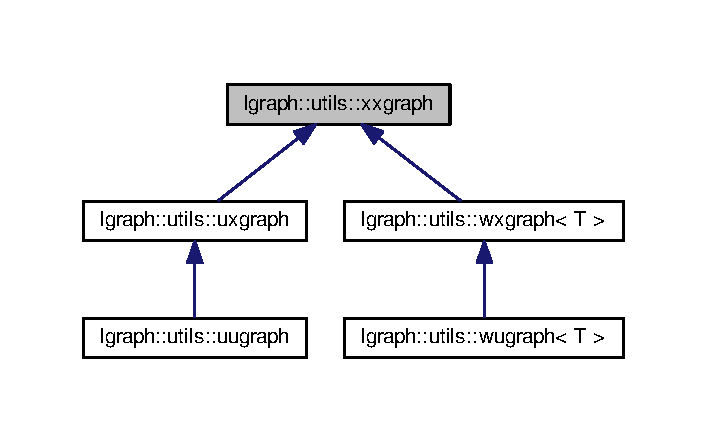
\includegraphics[width=350pt]{classlgraph_1_1utils_1_1xxgraph__inherit__graph}
\end{center}
\end{figure}
\subsection*{Public Member Functions}
\begin{DoxyCompactItemize}
\item 
\hyperlink{classlgraph_1_1utils_1_1xxgraph_a24cdfcb0cc82745b1ea44595b23f61bc}{xxgraph} ()\hypertarget{classlgraph_1_1utils_1_1xxgraph_a24cdfcb0cc82745b1ea44595b23f61bc}{}\label{classlgraph_1_1utils_1_1xxgraph_a24cdfcb0cc82745b1ea44595b23f61bc}

\begin{DoxyCompactList}\small\item\em Constructor. \end{DoxyCompactList}\item 
virtual \hyperlink{classlgraph_1_1utils_1_1xxgraph_a45d2fb9099f70fc2a8b1c651f4c6d6ce}{$\sim$xxgraph} ()\hypertarget{classlgraph_1_1utils_1_1xxgraph_a45d2fb9099f70fc2a8b1c651f4c6d6ce}{}\label{classlgraph_1_1utils_1_1xxgraph_a45d2fb9099f70fc2a8b1c651f4c6d6ce}

\begin{DoxyCompactList}\small\item\em Destructor. \end{DoxyCompactList}\item 
virtual void \hyperlink{classlgraph_1_1utils_1_1xxgraph_a2ac8b3e71fa0550248c692a19ea04d0d}{init} (size\+\_\+t n)=0
\begin{DoxyCompactList}\small\item\em Initialises the attributes of a graph with {\itshape n} nodes. \end{DoxyCompactList}\item 
size\+\_\+t \hyperlink{classlgraph_1_1utils_1_1xxgraph_af41baf2c098e872731ad646aeec1b382}{add\+\_\+node} ()
\begin{DoxyCompactList}\small\item\em Adds one node to the graph. \end{DoxyCompactList}\item 
size\+\_\+t \hyperlink{classlgraph_1_1utils_1_1xxgraph_af4f3782c1a55f73c6f34f2f2c26fb404}{add\+\_\+n\+\_\+nodes} (\hyperlink{namespacelgraph_1_1utils_a7bd66ede3805ef121bc2835bd48de0cf}{node} n)
\begin{DoxyCompactList}\small\item\em Adds {\itshape n} nodes to the graph. \end{DoxyCompactList}\item 
bool \hyperlink{classlgraph_1_1utils_1_1xxgraph_a026ab064c2be26790cc1f547be2157c9}{has\+\_\+node} (\hyperlink{namespacelgraph_1_1utils_a7bd66ede3805ef121bc2835bd48de0cf}{node} u) const \hypertarget{classlgraph_1_1utils_1_1xxgraph_a026ab064c2be26790cc1f547be2157c9}{}\label{classlgraph_1_1utils_1_1xxgraph_a026ab064c2be26790cc1f547be2157c9}

\begin{DoxyCompactList}\small\item\em Returns true if node {\itshape u} is in this graph. \end{DoxyCompactList}\item 
virtual bool \hyperlink{classlgraph_1_1utils_1_1xxgraph_a9e94100afc70b09049432f196550407c}{has\+\_\+edge} (\hyperlink{namespacelgraph_1_1utils_a7bd66ede3805ef121bc2835bd48de0cf}{node} u, \hyperlink{namespacelgraph_1_1utils_a7bd66ede3805ef121bc2835bd48de0cf}{node} v) const =0
\begin{DoxyCompactList}\small\item\em Returns true if there is an edge between nodes {\itshape u} and {\itshape v}. \end{DoxyCompactList}\item 
size\+\_\+t \hyperlink{classlgraph_1_1utils_1_1xxgraph_ad345f1fbf1dee34e1579b5aea9aef9b2}{n\+\_\+nodes} () const 
\begin{DoxyCompactList}\small\item\em Returns the number of nodes. \end{DoxyCompactList}\item 
size\+\_\+t \hyperlink{classlgraph_1_1utils_1_1xxgraph_af3f7c3835406c2cbf70479ae1c0253c9}{n\+\_\+edges} () const 
\begin{DoxyCompactList}\small\item\em Returns the number of edges. \end{DoxyCompactList}\item 
void \hyperlink{classlgraph_1_1utils_1_1xxgraph_a99f83387aa9f59b861e675251be5a3ad}{nodes} (vector$<$ \hyperlink{namespacelgraph_1_1utils_a7bd66ede3805ef121bc2835bd48de0cf}{node} $>$ \&all\+\_\+nodes) const \hypertarget{classlgraph_1_1utils_1_1xxgraph_a99f83387aa9f59b861e675251be5a3ad}{}\label{classlgraph_1_1utils_1_1xxgraph_a99f83387aa9f59b861e675251be5a3ad}

\begin{DoxyCompactList}\small\item\em Returns all nodes (as integers) \end{DoxyCompactList}\item 
const \hyperlink{namespacelgraph_1_1utils_a0f2ef47028a466d26841709e705390ac}{neighbourhood} \& \hyperlink{classlgraph_1_1utils_1_1xxgraph_a2c5332c4663c2d52828893f095a68202}{get\+\_\+neighbours} (\hyperlink{namespacelgraph_1_1utils_a7bd66ede3805ef121bc2835bd48de0cf}{node} u) const 
\begin{DoxyCompactList}\small\item\em Returns the neighbourhood of node u. \end{DoxyCompactList}\item 
size\+\_\+t \hyperlink{classlgraph_1_1utils_1_1xxgraph_af588aa4c68004a31aa143024cdb6dcc9}{degree} (\hyperlink{namespacelgraph_1_1utils_a7bd66ede3805ef121bc2835bd48de0cf}{node} u) const 
\begin{DoxyCompactList}\small\item\em Returns the number of neighbours of u. \end{DoxyCompactList}\item 
virtual bool \hyperlink{classlgraph_1_1utils_1_1xxgraph_a470b3fa2d6e37914d383de7d44f649e0}{is\+\_\+weighted} () const =0
\begin{DoxyCompactList}\small\item\em Returns whether the graph is weighted or unweighted. \end{DoxyCompactList}\item 
virtual bool \hyperlink{classlgraph_1_1utils_1_1xxgraph_a154376b6e55c4654622eb17ce738b5bb}{is\+\_\+directed} () const =0
\begin{DoxyCompactList}\small\item\em Returns whether the graph is directed or undirected. \end{DoxyCompactList}\item 
virtual bool \hyperlink{classlgraph_1_1utils_1_1xxgraph_a36206a20eb3f319bc01f1c07d16e0456}{read\+\_\+from\+\_\+file} (const string \&filename)=0\hypertarget{classlgraph_1_1utils_1_1xxgraph_a36206a20eb3f319bc01f1c07d16e0456}{}\label{classlgraph_1_1utils_1_1xxgraph_a36206a20eb3f319bc01f1c07d16e0456}

\begin{DoxyCompactList}\small\item\em Reads the graph from a file. \end{DoxyCompactList}\item 
virtual bool \hyperlink{classlgraph_1_1utils_1_1xxgraph_ac626dc5b5bac561bd103d9a346312b87}{read\+\_\+from\+\_\+file} (const char $\ast$filename)=0\hypertarget{classlgraph_1_1utils_1_1xxgraph_ac626dc5b5bac561bd103d9a346312b87}{}\label{classlgraph_1_1utils_1_1xxgraph_ac626dc5b5bac561bd103d9a346312b87}

\begin{DoxyCompactList}\small\item\em Reads the graph from a file. \end{DoxyCompactList}\item 
virtual bool \hyperlink{classlgraph_1_1utils_1_1xxgraph_aabf5361490305c1946d9084b1d9a026c}{store\+\_\+in\+\_\+file} (const string \&filename)=0\hypertarget{classlgraph_1_1utils_1_1xxgraph_aabf5361490305c1946d9084b1d9a026c}{}\label{classlgraph_1_1utils_1_1xxgraph_aabf5361490305c1946d9084b1d9a026c}

\begin{DoxyCompactList}\small\item\em Stores the graph in a file. \end{DoxyCompactList}\item 
virtual bool \hyperlink{classlgraph_1_1utils_1_1xxgraph_a5bb7620cd8721fc4b0d031230ab5c3b5}{store\+\_\+in\+\_\+file} (const char $\ast$filename)=0\hypertarget{classlgraph_1_1utils_1_1xxgraph_a5bb7620cd8721fc4b0d031230ab5c3b5}{}\label{classlgraph_1_1utils_1_1xxgraph_a5bb7620cd8721fc4b0d031230ab5c3b5}

\begin{DoxyCompactList}\small\item\em Stores the graph in a file. \end{DoxyCompactList}\item 
void \hyperlink{classlgraph_1_1utils_1_1xxgraph_a401454762f6b4b69f13ab0a10729c457}{get\+\_\+adjacency\+\_\+matrix} (vector$<$ vector$<$ bool $>$ $>$ \&adj\+\_\+mat) const \hypertarget{classlgraph_1_1utils_1_1xxgraph_a401454762f6b4b69f13ab0a10729c457}{}\label{classlgraph_1_1utils_1_1xxgraph_a401454762f6b4b69f13ab0a10729c457}

\begin{DoxyCompactList}\small\item\em Returns the adjacency matrix of this graph. \end{DoxyCompactList}\item 
void \hyperlink{classlgraph_1_1utils_1_1xxgraph_aff73f5ac4cd2732caa0c528eb1c1833c}{get\+\_\+degree\+\_\+sequence} (map$<$ size\+\_\+t, size\+\_\+t $>$ \&ds) const 
\begin{DoxyCompactList}\small\item\em Returns the degree sequence of the graph. \end{DoxyCompactList}\item 
size\+\_\+t \hyperlink{classlgraph_1_1utils_1_1xxgraph_ad4f25a8b29c6f26bc1567cb9c5a564ba}{n\+\_\+triangles} () const 
\begin{DoxyCompactList}\small\item\em Returns the number of triangles in this graph. \end{DoxyCompactList}\end{DoxyCompactItemize}
\subsection*{Protected Member Functions}
\begin{DoxyCompactItemize}
\item 
size\+\_\+t \hyperlink{classlgraph_1_1utils_1_1xxgraph_aac7ef2134cad9529869f1334de7892d9}{get\+\_\+neighbour\+\_\+position} (const \hyperlink{namespacelgraph_1_1utils_a0f2ef47028a466d26841709e705390ac}{neighbourhood} \&n, \hyperlink{namespacelgraph_1_1utils_a7bd66ede3805ef121bc2835bd48de0cf}{node} u) const 
\begin{DoxyCompactList}\small\item\em Returns the position of node {\itshape u\textquotesingle{}s} position in the neighbourhood {\itshape n}. \end{DoxyCompactList}\item 
void \hyperlink{classlgraph_1_1utils_1_1xxgraph_a2201aaff5e9ffa29a9b3abfde705dd46}{initialise\+\_\+adjacency\+\_\+list} (size\+\_\+t n)\hypertarget{classlgraph_1_1utils_1_1xxgraph_a2201aaff5e9ffa29a9b3abfde705dd46}{}\label{classlgraph_1_1utils_1_1xxgraph_a2201aaff5e9ffa29a9b3abfde705dd46}

\begin{DoxyCompactList}\small\item\em Initialise the list of neighbourhoods with {\itshape n} instances. \end{DoxyCompactList}\item 
void \hyperlink{classlgraph_1_1utils_1_1xxgraph_a6523402d0ec66918b95de23d2bee38fc}{clear\+\_\+adjacency\+\_\+list} ()\hypertarget{classlgraph_1_1utils_1_1xxgraph_a6523402d0ec66918b95de23d2bee38fc}{}\label{classlgraph_1_1utils_1_1xxgraph_a6523402d0ec66918b95de23d2bee38fc}

\begin{DoxyCompactList}\small\item\em Clear the list of neighbourhoods. \end{DoxyCompactList}\item 
void \hyperlink{classlgraph_1_1utils_1_1xxgraph_abd983125be7f2f2b9c812326a4a39e6d}{initialise\+\_\+parent\+\_\+graph} (size\+\_\+t n)
\begin{DoxyCompactList}\small\item\em Initialises the adjacency list of this graph. \end{DoxyCompactList}\item 
void \hyperlink{classlgraph_1_1utils_1_1xxgraph_a8d213a8dfe716d344dd51d1bd37c0e2c}{clear\+\_\+parent\+\_\+graph} ()
\begin{DoxyCompactList}\small\item\em Clears the adjacency list of this graph. \end{DoxyCompactList}\end{DoxyCompactItemize}
\subsection*{Protected Attributes}
\begin{DoxyCompactItemize}
\item 
vector$<$ \hyperlink{namespacelgraph_1_1utils_a0f2ef47028a466d26841709e705390ac}{neighbourhood} $>$ \hyperlink{classlgraph_1_1utils_1_1xxgraph_a1d5fda0d5aa89340f997428b982f966f}{adjacency\+\_\+list}\hypertarget{classlgraph_1_1utils_1_1xxgraph_a1d5fda0d5aa89340f997428b982f966f}{}\label{classlgraph_1_1utils_1_1xxgraph_a1d5fda0d5aa89340f997428b982f966f}

\begin{DoxyCompactList}\small\item\em The neighbourhood of every node. \end{DoxyCompactList}\item 
size\+\_\+t \hyperlink{classlgraph_1_1utils_1_1xxgraph_a217ebb1cd8946fedfbf94a9b22f7da48}{num\+\_\+edges}\hypertarget{classlgraph_1_1utils_1_1xxgraph_a217ebb1cd8946fedfbf94a9b22f7da48}{}\label{classlgraph_1_1utils_1_1xxgraph_a217ebb1cd8946fedfbf94a9b22f7da48}

\begin{DoxyCompactList}\small\item\em The amount of edges in this graph. \end{DoxyCompactList}\end{DoxyCompactItemize}


\subsection{Detailed Description}
Abstract class for the graph data structure. 

This interface requires the implementation of several methods to complete the implementation of a data structure for graphs that uses adjacency lists. It has only two attributes\+: \hyperlink{classlgraph_1_1utils_1_1xxgraph_a1d5fda0d5aa89340f997428b982f966f}{adjacency\+\_\+list}, that stores the adjacency list of each node, and \hyperlink{classlgraph_1_1utils_1_1xxgraph_a217ebb1cd8946fedfbf94a9b22f7da48}{num\+\_\+edges} that contains the number of edges in the graph. Depending on the type of graph implemented these two attributes should be modified accordingly. 

\subsection{Member Function Documentation}
\index{lgraph\+::utils\+::xxgraph@{lgraph\+::utils\+::xxgraph}!add\+\_\+n\+\_\+nodes@{add\+\_\+n\+\_\+nodes}}
\index{add\+\_\+n\+\_\+nodes@{add\+\_\+n\+\_\+nodes}!lgraph\+::utils\+::xxgraph@{lgraph\+::utils\+::xxgraph}}
\subsubsection[{\texorpdfstring{add\+\_\+n\+\_\+nodes(node n)}{add_n_nodes(node n)}}]{\setlength{\rightskip}{0pt plus 5cm}size\+\_\+t lgraph\+::utils\+::xxgraph\+::add\+\_\+n\+\_\+nodes (
\begin{DoxyParamCaption}
\item[{{\bf node}}]{n}
\end{DoxyParamCaption}
)}\hypertarget{classlgraph_1_1utils_1_1xxgraph_af4f3782c1a55f73c6f34f2f2c26fb404}{}\label{classlgraph_1_1utils_1_1xxgraph_af4f3782c1a55f73c6f34f2f2c26fb404}


Adds {\itshape n} nodes to the graph. 

The nodes are assigned consecutive, increasing values. \begin{DoxyReturn}{Returns}
Returns the index of the last node. 
\end{DoxyReturn}
\index{lgraph\+::utils\+::xxgraph@{lgraph\+::utils\+::xxgraph}!add\+\_\+node@{add\+\_\+node}}
\index{add\+\_\+node@{add\+\_\+node}!lgraph\+::utils\+::xxgraph@{lgraph\+::utils\+::xxgraph}}
\subsubsection[{\texorpdfstring{add\+\_\+node()}{add_node()}}]{\setlength{\rightskip}{0pt plus 5cm}size\+\_\+t lgraph\+::utils\+::xxgraph\+::add\+\_\+node (
\begin{DoxyParamCaption}
{}
\end{DoxyParamCaption}
)}\hypertarget{classlgraph_1_1utils_1_1xxgraph_af41baf2c098e872731ad646aeec1b382}{}\label{classlgraph_1_1utils_1_1xxgraph_af41baf2c098e872731ad646aeec1b382}


Adds one node to the graph. 

\begin{DoxyReturn}{Returns}
Returns the index of the new node 
\end{DoxyReturn}
\index{lgraph\+::utils\+::xxgraph@{lgraph\+::utils\+::xxgraph}!clear\+\_\+parent\+\_\+graph@{clear\+\_\+parent\+\_\+graph}}
\index{clear\+\_\+parent\+\_\+graph@{clear\+\_\+parent\+\_\+graph}!lgraph\+::utils\+::xxgraph@{lgraph\+::utils\+::xxgraph}}
\subsubsection[{\texorpdfstring{clear\+\_\+parent\+\_\+graph()}{clear_parent_graph()}}]{\setlength{\rightskip}{0pt plus 5cm}void lgraph\+::utils\+::xxgraph\+::clear\+\_\+parent\+\_\+graph (
\begin{DoxyParamCaption}
{}
\end{DoxyParamCaption}
)\hspace{0.3cm}{\ttfamily [protected]}}\hypertarget{classlgraph_1_1utils_1_1xxgraph_a8d213a8dfe716d344dd51d1bd37c0e2c}{}\label{classlgraph_1_1utils_1_1xxgraph_a8d213a8dfe716d344dd51d1bd37c0e2c}


Clears the adjacency list of this graph. 

The value \hyperlink{classlgraph_1_1utils_1_1xxgraph_a217ebb1cd8946fedfbf94a9b22f7da48}{num\+\_\+edges} is set to 0. \index{lgraph\+::utils\+::xxgraph@{lgraph\+::utils\+::xxgraph}!degree@{degree}}
\index{degree@{degree}!lgraph\+::utils\+::xxgraph@{lgraph\+::utils\+::xxgraph}}
\subsubsection[{\texorpdfstring{degree(node u) const }{degree(node u) const }}]{\setlength{\rightskip}{0pt plus 5cm}size\+\_\+t lgraph\+::utils\+::xxgraph\+::degree (
\begin{DoxyParamCaption}
\item[{{\bf node}}]{u}
\end{DoxyParamCaption}
) const}\hypertarget{classlgraph_1_1utils_1_1xxgraph_af588aa4c68004a31aa143024cdb6dcc9}{}\label{classlgraph_1_1utils_1_1xxgraph_af588aa4c68004a31aa143024cdb6dcc9}


Returns the number of neighbours of u. 


\begin{DoxyParams}{Parameters}
{\em u} & The node whose neighbourhood size we want \\
\hline
\end{DoxyParams}
\begin{DoxyReturn}{Returns}
Returns the size of the neighbourhood of {\itshape u}, that is, the size of the list in \hyperlink{classlgraph_1_1utils_1_1xxgraph_a1d5fda0d5aa89340f997428b982f966f}{adjacency\+\_\+list}\mbox{[}u\mbox{]} 
\end{DoxyReturn}
\begin{DoxyPrecond}{Precondition}
{\itshape u} must be a node from the graph 
\end{DoxyPrecond}
\index{lgraph\+::utils\+::xxgraph@{lgraph\+::utils\+::xxgraph}!get\+\_\+degree\+\_\+sequence@{get\+\_\+degree\+\_\+sequence}}
\index{get\+\_\+degree\+\_\+sequence@{get\+\_\+degree\+\_\+sequence}!lgraph\+::utils\+::xxgraph@{lgraph\+::utils\+::xxgraph}}
\subsubsection[{\texorpdfstring{get\+\_\+degree\+\_\+sequence(map$<$ size\+\_\+t, size\+\_\+t $>$ \&ds) const }{get_degree_sequence(map< size_t, size_t > &ds) const }}]{\setlength{\rightskip}{0pt plus 5cm}void lgraph\+::utils\+::xxgraph\+::get\+\_\+degree\+\_\+sequence (
\begin{DoxyParamCaption}
\item[{map$<$ size\+\_\+t, size\+\_\+t $>$ \&}]{ds}
\end{DoxyParamCaption}
) const}\hypertarget{classlgraph_1_1utils_1_1xxgraph_aff73f5ac4cd2732caa0c528eb1c1833c}{}\label{classlgraph_1_1utils_1_1xxgraph_aff73f5ac4cd2732caa0c528eb1c1833c}


Returns the degree sequence of the graph. 


\begin{DoxyParams}[1]{Parameters}
\mbox{\tt out}  & {\em ds} & A list of pairs\+: for each degree the amount of nodes in this graph that have that degree. The degree of a node is detailed in \hyperlink{classlgraph_1_1utils_1_1xxgraph_af588aa4c68004a31aa143024cdb6dcc9}{degree} \\
\hline
\end{DoxyParams}
\index{lgraph\+::utils\+::xxgraph@{lgraph\+::utils\+::xxgraph}!get\+\_\+neighbour\+\_\+position@{get\+\_\+neighbour\+\_\+position}}
\index{get\+\_\+neighbour\+\_\+position@{get\+\_\+neighbour\+\_\+position}!lgraph\+::utils\+::xxgraph@{lgraph\+::utils\+::xxgraph}}
\subsubsection[{\texorpdfstring{get\+\_\+neighbour\+\_\+position(const neighbourhood \&n, node u) const }{get_neighbour_position(const neighbourhood &n, node u) const }}]{\setlength{\rightskip}{0pt plus 5cm}size\+\_\+t lgraph\+::utils\+::xxgraph\+::get\+\_\+neighbour\+\_\+position (
\begin{DoxyParamCaption}
\item[{const {\bf neighbourhood} \&}]{n, }
\item[{{\bf node}}]{u}
\end{DoxyParamCaption}
) const\hspace{0.3cm}{\ttfamily [protected]}}\hypertarget{classlgraph_1_1utils_1_1xxgraph_aac7ef2134cad9529869f1334de7892d9}{}\label{classlgraph_1_1utils_1_1xxgraph_aac7ef2134cad9529869f1334de7892d9}


Returns the position of node {\itshape u\textquotesingle{}s} position in the neighbourhood {\itshape n}. 

If the position is equal to the number of elements of the list {\itshape n} then {\itshape u} is in the list. Performs a linear search to find it. 
\begin{DoxyParams}{Parameters}
{\em n} & The neighbourhood of a node in the graph \\
\hline
{\em u} & The node to look for in the neighbourhood \\
\hline
\end{DoxyParams}
\begin{DoxyReturn}{Returns}
Returns a value equal to the number of elements in the list {\itshape n} if node {\itshape u} is not in it. Returns a value smaller than that if otherwise. 
\end{DoxyReturn}
\index{lgraph\+::utils\+::xxgraph@{lgraph\+::utils\+::xxgraph}!get\+\_\+neighbours@{get\+\_\+neighbours}}
\index{get\+\_\+neighbours@{get\+\_\+neighbours}!lgraph\+::utils\+::xxgraph@{lgraph\+::utils\+::xxgraph}}
\subsubsection[{\texorpdfstring{get\+\_\+neighbours(node u) const }{get_neighbours(node u) const }}]{\setlength{\rightskip}{0pt plus 5cm}const {\bf neighbourhood} \& lgraph\+::utils\+::xxgraph\+::get\+\_\+neighbours (
\begin{DoxyParamCaption}
\item[{{\bf node}}]{u}
\end{DoxyParamCaption}
) const}\hypertarget{classlgraph_1_1utils_1_1xxgraph_a2c5332c4663c2d52828893f095a68202}{}\label{classlgraph_1_1utils_1_1xxgraph_a2c5332c4663c2d52828893f095a68202}


Returns the neighbourhood of node u. 


\begin{DoxyParams}{Parameters}
{\em u} & The node whose neighbourhood we want \\
\hline
\end{DoxyParams}
\begin{DoxyPrecond}{Precondition}
{\itshape u} must be a node from the graph 
\end{DoxyPrecond}
\index{lgraph\+::utils\+::xxgraph@{lgraph\+::utils\+::xxgraph}!has\+\_\+edge@{has\+\_\+edge}}
\index{has\+\_\+edge@{has\+\_\+edge}!lgraph\+::utils\+::xxgraph@{lgraph\+::utils\+::xxgraph}}
\subsubsection[{\texorpdfstring{has\+\_\+edge(node u, node v) const =0}{has_edge(node u, node v) const =0}}]{\setlength{\rightskip}{0pt plus 5cm}virtual bool lgraph\+::utils\+::xxgraph\+::has\+\_\+edge (
\begin{DoxyParamCaption}
\item[{{\bf node}}]{u, }
\item[{{\bf node}}]{v}
\end{DoxyParamCaption}
) const\hspace{0.3cm}{\ttfamily [pure virtual]}}\hypertarget{classlgraph_1_1utils_1_1xxgraph_a9e94100afc70b09049432f196550407c}{}\label{classlgraph_1_1utils_1_1xxgraph_a9e94100afc70b09049432f196550407c}


Returns true if there is an edge between nodes {\itshape u} and {\itshape v}. 

\begin{DoxyPrecond}{Precondition}
{\itshape u} and {\itshape v} must be in the graph 
\end{DoxyPrecond}


Implemented in \hyperlink{classlgraph_1_1utils_1_1wdgraph_ac74f172c5a6bdbf56ac5a4013fae880a}{lgraph\+::utils\+::wdgraph$<$ T $>$}, \hyperlink{classlgraph_1_1utils_1_1wugraph_a5d729aece87dbda408211b12ad4856d1}{lgraph\+::utils\+::wugraph$<$ T $>$}, \hyperlink{classlgraph_1_1utils_1_1udgraph_aebc98d234955028116978eff9c13445b}{lgraph\+::utils\+::udgraph}, and \hyperlink{classlgraph_1_1utils_1_1uugraph_a1970a2f371f20284478246a83292f9bb}{lgraph\+::utils\+::uugraph}.

\index{lgraph\+::utils\+::xxgraph@{lgraph\+::utils\+::xxgraph}!init@{init}}
\index{init@{init}!lgraph\+::utils\+::xxgraph@{lgraph\+::utils\+::xxgraph}}
\subsubsection[{\texorpdfstring{init(size\+\_\+t n)=0}{init(size_t n)=0}}]{\setlength{\rightskip}{0pt plus 5cm}virtual void lgraph\+::utils\+::xxgraph\+::init (
\begin{DoxyParamCaption}
\item[{size\+\_\+t}]{n}
\end{DoxyParamCaption}
)\hspace{0.3cm}{\ttfamily [pure virtual]}}\hypertarget{classlgraph_1_1utils_1_1xxgraph_a2ac8b3e71fa0550248c692a19ea04d0d}{}\label{classlgraph_1_1utils_1_1xxgraph_a2ac8b3e71fa0550248c692a19ea04d0d}


Initialises the attributes of a graph with {\itshape n} nodes. 

First, it clears all the memory allocated so far. Then, initialises all the attributes so that it can store all the necessary information. 
\begin{DoxyParams}{Parameters}
{\em n} & Number of nodes of the graph \\
\hline
\end{DoxyParams}


Implemented in \hyperlink{classlgraph_1_1utils_1_1wxgraph_a566ae9fe69209230ef159ed350ab8f7f}{lgraph\+::utils\+::wxgraph$<$ T $>$}, and \hyperlink{classlgraph_1_1utils_1_1uxgraph_ab1e7ab39be6e8ca6149eef47dd51b155}{lgraph\+::utils\+::uxgraph}.

\index{lgraph\+::utils\+::xxgraph@{lgraph\+::utils\+::xxgraph}!initialise\+\_\+parent\+\_\+graph@{initialise\+\_\+parent\+\_\+graph}}
\index{initialise\+\_\+parent\+\_\+graph@{initialise\+\_\+parent\+\_\+graph}!lgraph\+::utils\+::xxgraph@{lgraph\+::utils\+::xxgraph}}
\subsubsection[{\texorpdfstring{initialise\+\_\+parent\+\_\+graph(size\+\_\+t n)}{initialise_parent_graph(size_t n)}}]{\setlength{\rightskip}{0pt plus 5cm}void lgraph\+::utils\+::xxgraph\+::initialise\+\_\+parent\+\_\+graph (
\begin{DoxyParamCaption}
\item[{size\+\_\+t}]{n}
\end{DoxyParamCaption}
)\hspace{0.3cm}{\ttfamily [protected]}}\hypertarget{classlgraph_1_1utils_1_1xxgraph_abd983125be7f2f2b9c812326a4a39e6d}{}\label{classlgraph_1_1utils_1_1xxgraph_abd983125be7f2f2b9c812326a4a39e6d}


Initialises the adjacency list of this graph. 

The value \hyperlink{classlgraph_1_1utils_1_1xxgraph_a217ebb1cd8946fedfbf94a9b22f7da48}{num\+\_\+edges} is set to 0. \index{lgraph\+::utils\+::xxgraph@{lgraph\+::utils\+::xxgraph}!is\+\_\+directed@{is\+\_\+directed}}
\index{is\+\_\+directed@{is\+\_\+directed}!lgraph\+::utils\+::xxgraph@{lgraph\+::utils\+::xxgraph}}
\subsubsection[{\texorpdfstring{is\+\_\+directed() const =0}{is_directed() const =0}}]{\setlength{\rightskip}{0pt plus 5cm}virtual bool lgraph\+::utils\+::xxgraph\+::is\+\_\+directed (
\begin{DoxyParamCaption}
{}
\end{DoxyParamCaption}
) const\hspace{0.3cm}{\ttfamily [pure virtual]}}\hypertarget{classlgraph_1_1utils_1_1xxgraph_a154376b6e55c4654622eb17ce738b5bb}{}\label{classlgraph_1_1utils_1_1xxgraph_a154376b6e55c4654622eb17ce738b5bb}


Returns whether the graph is directed or undirected. 

\begin{DoxyReturn}{Returns}
Returns true if the graph is directed. Returns false if otherwise. 
\end{DoxyReturn}


Implemented in \hyperlink{classlgraph_1_1utils_1_1wdgraph_a5eee58626ec0aa8428436a859d601741}{lgraph\+::utils\+::wdgraph$<$ T $>$}, \hyperlink{classlgraph_1_1utils_1_1wugraph_a3ed8cd6b1d499fd3f36ec6c1cb2845d3}{lgraph\+::utils\+::wugraph$<$ T $>$}, \hyperlink{classlgraph_1_1utils_1_1udgraph_aa6fc318096cc4b577374f002b07ab49b}{lgraph\+::utils\+::udgraph}, and \hyperlink{classlgraph_1_1utils_1_1uugraph_a20a86c5b56527e8abcbb90bae95d6605}{lgraph\+::utils\+::uugraph}.

\index{lgraph\+::utils\+::xxgraph@{lgraph\+::utils\+::xxgraph}!is\+\_\+weighted@{is\+\_\+weighted}}
\index{is\+\_\+weighted@{is\+\_\+weighted}!lgraph\+::utils\+::xxgraph@{lgraph\+::utils\+::xxgraph}}
\subsubsection[{\texorpdfstring{is\+\_\+weighted() const =0}{is_weighted() const =0}}]{\setlength{\rightskip}{0pt plus 5cm}virtual bool lgraph\+::utils\+::xxgraph\+::is\+\_\+weighted (
\begin{DoxyParamCaption}
{}
\end{DoxyParamCaption}
) const\hspace{0.3cm}{\ttfamily [pure virtual]}}\hypertarget{classlgraph_1_1utils_1_1xxgraph_a470b3fa2d6e37914d383de7d44f649e0}{}\label{classlgraph_1_1utils_1_1xxgraph_a470b3fa2d6e37914d383de7d44f649e0}


Returns whether the graph is weighted or unweighted. 

\begin{DoxyReturn}{Returns}
Returns true if the graph is weighted. Returns false if otherwise. 
\end{DoxyReturn}


Implemented in \hyperlink{classlgraph_1_1utils_1_1wxgraph_adda596cfbf72080d46ab445679fe092f}{lgraph\+::utils\+::wxgraph$<$ T $>$}, and \hyperlink{classlgraph_1_1utils_1_1uxgraph_ae1c3f40bb80ab20c2de96735ccde7b3f}{lgraph\+::utils\+::uxgraph}.

\index{lgraph\+::utils\+::xxgraph@{lgraph\+::utils\+::xxgraph}!n\+\_\+edges@{n\+\_\+edges}}
\index{n\+\_\+edges@{n\+\_\+edges}!lgraph\+::utils\+::xxgraph@{lgraph\+::utils\+::xxgraph}}
\subsubsection[{\texorpdfstring{n\+\_\+edges() const }{n_edges() const }}]{\setlength{\rightskip}{0pt plus 5cm}size\+\_\+t lgraph\+::utils\+::xxgraph\+::n\+\_\+edges (
\begin{DoxyParamCaption}
{}
\end{DoxyParamCaption}
) const}\hypertarget{classlgraph_1_1utils_1_1xxgraph_af3f7c3835406c2cbf70479ae1c0253c9}{}\label{classlgraph_1_1utils_1_1xxgraph_af3f7c3835406c2cbf70479ae1c0253c9}


Returns the number of edges. 

\begin{DoxyReturn}{Returns}
Returns the value \hyperlink{classlgraph_1_1utils_1_1xxgraph_a217ebb1cd8946fedfbf94a9b22f7da48}{num\+\_\+edges} 
\end{DoxyReturn}
\index{lgraph\+::utils\+::xxgraph@{lgraph\+::utils\+::xxgraph}!n\+\_\+nodes@{n\+\_\+nodes}}
\index{n\+\_\+nodes@{n\+\_\+nodes}!lgraph\+::utils\+::xxgraph@{lgraph\+::utils\+::xxgraph}}
\subsubsection[{\texorpdfstring{n\+\_\+nodes() const }{n_nodes() const }}]{\setlength{\rightskip}{0pt plus 5cm}size\+\_\+t lgraph\+::utils\+::xxgraph\+::n\+\_\+nodes (
\begin{DoxyParamCaption}
{}
\end{DoxyParamCaption}
) const}\hypertarget{classlgraph_1_1utils_1_1xxgraph_ad345f1fbf1dee34e1579b5aea9aef9b2}{}\label{classlgraph_1_1utils_1_1xxgraph_ad345f1fbf1dee34e1579b5aea9aef9b2}


Returns the number of nodes. 

\begin{DoxyReturn}{Returns}
Returns the size of \hyperlink{classlgraph_1_1utils_1_1xxgraph_a1d5fda0d5aa89340f997428b982f966f}{adjacency\+\_\+list} 
\end{DoxyReturn}
\index{lgraph\+::utils\+::xxgraph@{lgraph\+::utils\+::xxgraph}!n\+\_\+triangles@{n\+\_\+triangles}}
\index{n\+\_\+triangles@{n\+\_\+triangles}!lgraph\+::utils\+::xxgraph@{lgraph\+::utils\+::xxgraph}}
\subsubsection[{\texorpdfstring{n\+\_\+triangles() const }{n_triangles() const }}]{\setlength{\rightskip}{0pt plus 5cm}size\+\_\+t lgraph\+::utils\+::xxgraph\+::n\+\_\+triangles (
\begin{DoxyParamCaption}
{}
\end{DoxyParamCaption}
) const}\hypertarget{classlgraph_1_1utils_1_1xxgraph_ad4f25a8b29c6f26bc1567cb9c5a564ba}{}\label{classlgraph_1_1utils_1_1xxgraph_ad4f25a8b29c6f26bc1567cb9c5a564ba}


Returns the number of triangles in this graph. 

\begin{DoxyReturn}{Returns}
Returns the number of cycles of length 3 
\end{DoxyReturn}


The documentation for this class was generated from the following files\+:\begin{DoxyCompactItemize}
\item 
lgraph/data\+\_\+structures/xxgraph.\+hpp\item 
lgraph/data\+\_\+structures/xxgraph.\+cpp\end{DoxyCompactItemize}

%--- End generated contents ---

% Index
\backmatter
\newpage
\phantomsection
\clearemptydoublepage
\addcontentsline{toc}{chapter}{Index}
\printindex

\end{document}
